%%%%%%%%%%%%%%%%%%%%%%%%%%%%%%%
% Inlcude preable
%%% Definition der Dokumentklasse für A4-Papier und 12 Punkte Schriftgröße.
%%% Ränder sind für Klebebindung sowohl im A4- als auch im herunterskalierten
%%% A5-Ausdruck optimiert.
\documentclass[a4paper,titlepage,bibliography=totoc,12pt,BCOR=17mm,DIV=12,headinclude,footinclude=false]{scrbook}

\usepackage[utf8]{inputenc}

\usepackage{easy-todo}

\usepackage{tikz}
\usetikzlibrary{decorations.markings,decorations.text,calc,arrows,positioning,shapes}
\tikzstyle{decision} = [diamond, draw, fill=blue!20, text width=4.5em, text badly centered, node distance=2cm, inner sep=0pt]
\tikzstyle{block} = [rectangle, draw, fill=blue!20, text width=0.8\textwidth, text centered, rounded corners, minimum height=3em]
\tikzstyle{block2} = [rectangle, draw, text centered, rounded corners, minimum height=2em]
\tikzstyle{line} = [draw, -latex']
\tikzstyle{cloud} = [draw, ellipse,fill=red!20, node distance=3cm, minimum height=2em]
\tikzstyle{process} = [rectangle, minimum width=3cm, minimum height=2em, text centered, draw=black, fill=orange!30]

\usepackage{minibox}
\usepackage{mdframed}
\mdfsetup{
  skipabove=\baselineskip,
  skipbelow=\baselineskip
}


%%%%%%%%%%%%%%%%%%%%%%%%%%%%%%
%%% Math symbols etc
\usepackage{amsmath,amsfonts,amssymb}
\usepackage{bbold}
\usepackage{slashed}
\usepackage{physics}
\usepackage{booktabs}
\usepackage{tabularx,bigdelim}
\usepackage{multirow}
\usepackage{xfrac}
\usepackage{siunitx}
\usepackage{mathtools}

%%%%%%%%%%%%%%%%%%%%%%%%%%%%%%
%%% Grafics
\usepackage{graphicx}
\usepackage{caption}
%\usepackage{subcaption}
%%% Sidecap: Bildbeschriftung seitlich neben dem Bild
%\usepackage{sidecap}
\usepackage[caption=false]{subfig}
\usepackage{wrapfig}

\usepackage{placeins}
\usepackage{adjustbox}

%%%%%%%%%%%%%%%%%%%%%%%%%%%%%%
%%% Header
%%% Fancyhdr: Nette Kopf- und Fusszeilen, werden weiter unten definiert.
\usepackage{fancyhdr}
%%% Definition der Kopf- und Fussleisten
\pagestyle{fancy}
\renewcommand{\chaptermark}[1]{% Kopfzeilen in Groß-/Kleinschreibung
\markboth{%
\chaptername\ \thechapter.%
\ #1}{}}
\renewcommand{\sectionmark}[1]{% Kopfzeilen in Groß-/Kleinschreibung
\markright{%
\thesection.%
\ #1}}


\usepackage{titlesec, blindtext, color} 

%\definecolor{gray75}{gray}{0.75}
%\newcommand{\hsp}{\hspace{20pt}}
%\titleformat{\chapter}[hang]{\Huge\bfseries}{\thechapter\hsp\textcolor{gray75}{|}\hsp}{0pt}{\Huge\bfseries}

%\renewcommand{\thechapter}{\Roman{chapter}}
\titleformat{\chapter}[display]
{\bfseries\Large}
{\filleft\MakeUppercase{\chaptertitlename} \Huge\thechapter}
{2ex}
{\titlerule
  \vspace{1ex}%
\filright}
[\vspace{2ex}%
\titlerule]

\titlespacing{\chapter}{0cm}{-1cm}{0.5cm}[0cm]

\titlespacing{\paragraph}{%
  0pt}{%              left margin
  0.5\baselineskip}{% space before (vertical)
  1em}%               space after (horizontal)


%\titleformat{\chapter}[display]
%  {\bfseries\Large}
%  {\filright\MakeUppercase{\chaptertitlename} \Huge\thechapter}
%  {1ex}
%  {\titlerule\vspace{1ex}\filleft}
%  [\vspace{1ex}\titlerule]

%%% Seitennumerierung vor dem eigentlichen Inhalt in römischen Zahlen
\pagenumbering{roman}

%%% Vermeidung von Hurenkindern und Schusterjungen
\clubpenalty = 10000  % schliesst Schusterjungen aus
\widowpenalty = 10000 % schliesst Hurenkinder aus


%%%%%%%%%%%%%%%%%%%%%%%%%%%%%%
%%% Einige Pakete für eine schöne Titelseite
\usepackage{everyshi,eso-pic,calc,ifthen,sty/wallpaper}
\usepackage{sty/diplomarbeit}

%%%%%%%%%%%%%%%%%%%%%%%%%%%%%%

%%% Eineinhalbfachen Zeilenabstand nutzen (Vorgabe Prüfungsamt)
\usepackage{setspace}
%\onehalfspacing
\typearea[current]{last}



\usepackage[%
  pdftitle={Scattering Amplitudes with Multi-Loop Generalized Numerical Unitarity Method},%
  pdfauthor={Vasily Sotnikov}%
]{hyperref}

\hypersetup{
    colorlinks=true,
    allcolors={blue!60!black}
    %linkcolor={red!50!black},
    %citecolor={blue!50!black},
    %urlcolor={blue!80!black}
}

%%% Mehrere aufeinanderfolgend numerierte Zitate mit einem Bindestrich zusammen
%%% fassen (z.B. [1-5] statt [1,2,3,4,5]).
\usepackage[numbers,sort&compress]{natbib}
\usepackage{doi}

%%% Hypernat beseitigt Fehler durch das
%%% Paket Hyperref in Zusammenhang mit dieser Kompression.
%\usepackage{hypernat}


%%%%%%%%%%%%%%%%%%%%%%%%%%%%%%

%-- Defines a CAPTION for a set of equations and numbers
%   the set of equations is numbered
% note: the caption adapts the text alignment to the length. 
\newcounter{captionedequationset} %numbering
\newdimen\captionlength
\newcommand{\captionedequationset}[1]{
    \refstepcounter{figure}% Step counter
    \setlength{\captionlength}{\widthof{#1}} %
    \addtolength{\captionlength}{\widthof{Figure~\thefigure: }}
    %If the caption is shorter than the line width then
    % the caption is centred, otherwise is flushed left.
    \ifthenelse{\lengthtest{\captionlength < \linewidth }} %
    {\begin{center}
            Figure~\thefigure: #1
        \end{center}} 
    { \begin{flushleft} 
        Figure~\thefigure: #1 %
        \end{flushleft}}}




%%%%%%%%%%%%%%%%%%%%%%%%%%%%%%
%%%%%%%%%%%%%%%%%%%%%%%%%%%%%%
%  NOT USE CURRENTLY
%%%%%%%%%%%%%%%%%%%%%%%%%%%%%%
%%%%%%%%%%%%%%%%%%%%%%%%%%%%%%
%%% Fancyref: Vereinfachte Referenzen. Labels werden im Format "PRÄFIX:LABEL"
%%%           erstellt. Dann wird mit \fref{PRÄFIX:LABEL} ein Verweis der Form
%%%           z.B. "Kapitel 4" oder "Abschnitt 4.5" statt nur "4" oder "4.5"
%%%           erstellt.
%%%           ACHTUNG: Fehlt im Label im \fref-Kommando das Präfix und der
%%%           Doppelpunkt, kommt es zu Fehlermeldungen, die ein fehlendes "}"
%%%           beklagen!
%%%           Liste der Präfixe und zugehöriger Objekte:
%%%           Object      Prefix
%%%           Chapter     chap
%%%           Section     sec
%%%           Equation    eq
%%%           Figure      fig
%%%           Table       tab
%%%           Enumeration enum
%%%           Footnote    fn
%%%           Anhang*     apx
%%%           *) Selbst definiertes Präfix

%%%\usepackage[german,plain]{fancyref}
%%% 
%%%\newcommand*{\fancyrefapxlabelprefix}{apx}
%%%\frefformat{plain}{\fancyrefapxlabelprefix}{%
%%%    Anhang\fancyrefdefaultspacing#1%
%%%}%
%%%\Frefformat{plain}{\fancyrefapxlabelprefix}{%
%%%    Anhang\fancyrefdefaultspacing#1%
%%%}%

%%%%%%%%%%%%%%%%%%%%%%%%%%%%%%
%%% URL: Zur besseren Darstellung von URLs z.B. in Literaturquellen (einbindbar
%%%      z.B. über "howpublished = \url{URL}")
%\usepackage{url}

%%%%%%%%%%%%%%%%%%%%%%%%%%%%%%
%%% Hyphenat: Problemlöser für Trennungsprobleme: TeX trennt keine Wörter, die
%%%           bereits einen Bindestrich beinhalten (z.B. Wasserstoff-Atom).
%%%           Um die automatische Worttrennung auch bei solchen Wörtern zu 
%%%           aktivieren, ersetzt man einfach den Bindestrich durch das 
%%%           Kommando \hyp{}, also z.B. "Wasserstoff\hyp{}Atom".
%\usepackage{hyphenat}

%%%%%%%%%%%%%%%%%%%%%%%%%%%%%%

%%% Mit diesen Kommandos kann man eigene Kapitel- und Sektionskopfzeilen
%%% einbinden. Anwendung:
%%%    \chapter{Langer Kapitelname}
%%%    \shortchapter{Kurzer Kapitelname für Kopfzeile}
%\newcommand{\shortchapter}[1]{% Erstellt eine eigene Kapitel-Kopfzeile
%\markboth{%
%\chaptername\ \thechapter.%
%\ #1}{}}
%\newcommand{\shortsection}[1]{% Erstellt eine eigene Sektions-Kopfzeile
%\markright{%
%\thesection.%
%\ #1}}

%%%%%%%%%%%%%%%%%%%%%%%%%%%%%%

\usepackage{enumitem}

\usepackage{cmap}
\usepackage{indentfirst}

% for ranges of equations
\usepackage{cleveref}

\graphicspath{{figures/}}


%%%%%%%%%%%%%%%%%%%%%%%%%%%%%%
% Own defs etc
%----------------------------------------------------------------------------------------------
\textheight = 24cm
\textwidth = 16cm
\oddsidemargin = -5pt
\topmargin = -1.5cm
\parskip = 10pt
%----------------------------------------------------------------------------------------------
%\numberwithin{equation}{section}
%----------------------------------------------------------------------------------------------


\def\recola{\texttt{RECOLA}}
\def\OL{\texttt{OpenLoops}}
%\def\BH{\texttt{BlackHat}}
\renewcommand{\textfraction}{0}
\renewcommand{\topfraction}{1}
\renewcommand{\bottomfraction}{1}
\newcommand{\BlackHat}{\texttt{BlackHat}}
%\newcommand{\BHM}{{\textsc BlackHat\textunderscore Massive}}
\newcommand{\PYTHIA}{\textsc{Pythia}}
\newcommand{\HELACNLO}{\textsc{HELAC-NLO}}
\newcommand{\NLOJet}{\textsc{NLOJET++}}
\newcommand{\SHERPA}{\texttt{SHERPA}}
\newcommand{\MCFM}{\texttt{MCFM}}
\newcommand{\AMEGIC}{\texttt{AMEGIC++}}
\newcommand{\COMIX}{\texttt{COMIX}}
\newcommand{\SISCone}{\texttt{SISCone}}
\newcommand{\ntuple}{{$n$-tuple}}
\newcommand{\ntuples}{{$n$-tuples}}
\newcommand{\Ntuple}{{$N$-tuple}}
\newcommand{\Ntuples}{{$N$-tuples}}
\newcommand{\mc}[1]{\mathcal{#1}}
\newcommand{\FO}{{4FNS}}
\newcommand{\FI}{{5FNS}}

\newcommand{\Abs}[1]{\vert #1 \vert^2}
\newcommand{\Ree}[2]{2\Re({#1}^{*} #2)}


\def\gjn{$\gamma\,\!+\,n$}
\def\jet{{\textrm jet}}
\def\kT{k_{\textrm T}}
\def\pT{p_{\textrm T}}
\def\pTn#1{p_{{\textrm T}#1}}
\def\pTmin{\pT^{\text{min}}}
\def\pTV{\pT^V}
\def\pTW{\pT^W}
\def\root{{\textsc root}}
\def\Ord{{\cal O}}

\def\pres#1#2{\prescript{(#2)}{}{#1}}
\def\lgs{\text{SO}(D_s-4)}

\def\llg{\Lambda_{\frac{1}{2},\text{hd}}^{\phantom{\dagger}}}
\def\llgd{\Lambda_{\frac{1}{2},\text{hd}}^\dagger}

\def\sma{$\mathcal{S}$-matrix}


\def\dof{d.o.f.}
\def\ttj{$t\bar{t}j$}
\def\ttjj{$t\bar{t}jj$}
\def\ttjjj{$t\bar{t}jjj$}
\def\ttbb{$t\bar{t}b\bar{b}$}
\def\ttbbj{$t\bar{t}b\bar{b}j$}
        \def\ggtottbbg{$gg\rightarrow t\bar{t}b\bar{b}g$}
\def\qqtottbbg{$q\bar{q}\rightarrow t\bar{t}b\bar{b}g$}
\def\qgtottbbq{$qg\rightarrow t\bar{t}b\bar{b}\bar{q}$}
\def\Wbbn[#1]{$Wb\bar{b}+n$-jet ($n=0,1,2,3$)}
\def\Wbbnj[#1]{$Wb\bar{b}+#1$-jet}
\def\Wbb{$Wb\bar{b}$}
\def\Wjj{$Wjj$}
\def\Wjjj{$Wjjj$}
\def\Wjjjj{$Wjjjj$}
\def\Wbbp{$W^+b\bar{b}$}
\def\Wbbm{$W^-b\bar{b}$}
\def\Wbbpm{$W^\pm b\bar{b}$}
\def\Wbbj{$Wb\bar{b}j$}
\def\Wbbjj{$Wb\bar{b}jj$}
\def\Wbbjjj{$Wb\bar{b}jjj$}
\def\Zbb{$Zb\bar{b}$}
\def\Zbbj{$Zb\bar{b}j$}
\def\Zbbjj{$Zb\bar{b}jj$}
\def\ggtoWbbg{$gg\rightarrow Wb\bar{b}g$}
\def\qqtoWbbg{$q\bar{q}\rightarrow Wb\bar{b}g$}
\def\qgtoWbbq{$qg\rightarrow Wb\bar{b}\bar{q}$}
\def\ggtoWbb{$gg\rightarrow Wb\bar{b}$}
\def\qqtoWbb{$q\bar{q}\rightarrow Wb\bar{b}$}
\def\ggtoWbbgg{$gg\rightarrow Wb\bar{b}gg$}
\def\ggtoWbbqq{$gg\rightarrow Wb\bar{b}q\bar{q}$}
\def\qqtoWbbgg{$q\bar{q}\rightarrow Wb\bar{b}gg$}
\def\qqtoWbbqq{$qq\rightarrow Wb\bar{b}\bar{q}\bar{q}$}
\def\qqbtoWbbqqb{$q\bar{q}\rightarrow Wb\bar{b}q\bar{q}$}
\def\qgtoWbbqg{$qg\rightarrow Wb\bar{b}\bar{q}g$}
\def\qqtoWbbggg{$q\bar{q}\rightarrow Wb\bar{b}ggg$}
\def\qqtoWbbqqg{$q\bar{q}\rightarrow Wb\bar{b}q\bar{q}g$}


\def\murt{\tilde{\mu}_R^2}


\def\MINLO{\texttt{MiNLO}}
\def\MILO{\texttt{MiLO}}
\def\muMILO{\mu_{\tiny\mathrm MiLO}}
\def\muMINLO{\mu_{\tiny\mathrm MiNLO}}

\def\HTpartonic{{\hat H}_{\mathrm T}}
\def\HTpartonicp{{\hat H}_{\mathrm T}'}
\def\HTpartonicpp{{\hat S}_{\mathrm T}}


\def\HT{H_{\textrm T}}
\def\HTjets{H_{\textrm T}^{\textrm jets}}
\def\hatMNLO{\widehat{d\sigma}_V^{(1)}}
\def\MT{M_{\textrm T}}
\def\MINLOp{\texttt{MiNLO$^\prime$}}
\def\MILOp{\texttt{MiLO$^\prime$}}
\def\MILNLO{\texttt{Mi(N)LO}}
\def\MILNLOp{\texttt{Mi(N)LO$^\prime$}}
\def\HTpp{{\hat H}_{\textrm T}''}
\def\KDHTp{{\texttt KD}}
\def\KDHTpp{{\texttt KD2}}
\def\KDHTppp{{\texttt KD3}}
\def\muMILOp{\mu_{\tiny\mathrm MiLO^\prime}}
\def\muMINLOp{\mu_{\tiny\mathrm MiNLO^\prime}}


\def\akt{anti-$k_T$}
\def\asms[#1]{\alpha_s^{\MSb}(#1)}
\def\MSb{\overline{\text{MS}}}
\def\ew{electroweak}

\def\gmna{$g^{\mu\nu}$}
\def\gmn{g^{\mu\nu}}
\def\gm{\gamma^\mu}
\def\gum{\gamma_\mu}
\def\gn{\gamma^\nu}
\def\g5{\gamma_5}
\def\une{_{[n_\epsilon-2\epsilon]}}
\def\ue{_{[-2\epsilon]}}
\def\u4{_{[4]}}
\def\u4{_{[4]}}

\def\alps{\alpha_s}
\def\alpf{\alpha_f}

\newtheorem{myrule}{Rule}
\newtheorem{mydef}{Definition}


\newsavebox\myboxA
\newsavebox\myboxB
\newlength\mylenA

\makeatletter
\newcommand*\xoverline[2][0.75]{%
    \sbox{\myboxA}{$\m@th#2$}%
    \setbox\myboxB\null% Phantom box
    \ht\myboxB=\ht\myboxA%
    \dp\myboxB=\dp\myboxA%
    \wd\myboxB=#1\wd\myboxA% Scale phantom
    \sbox\myboxB{$\m@th\overline{\copy\myboxB}$}%  Overlined phantom
    \setlength\mylenA{\the\wd\myboxA}%   calc width diff
    \addtolength\mylenA{-\the\wd\myboxB}%
    \ifdim\wd\myboxB<\wd\myboxA%
       \rlap{\hskip 0.5\mylenA\usebox\myboxB}{\usebox\myboxA}%
    \else
        \hskip -0.5\mylenA\rlap{\usebox\myboxA}{\hskip 0.5\mylenA\usebox\myboxB}%
    \fi
}
\makeatother



\newcommand\dt{D_{\text{t}}}
\newcommand\dtt{\widetilde{D}_{\text{t}}}
\newcommand\dttindex{$\dtt$-index}

\providecommand\tr{}
\renewcommand\tr[2][]{
  \mathrm{Tr}_{#1} \left[ #2 \right]
}
\newcommand\trf[1][]{
  \mathrm{Tr} \left[ #1 \right]
}


\def\QS#1{\mathrm{QS}_{[#1]}}
\def\Sf{\mathrm{S}_{[4]}}

\def\gm#1#2#3{\prescript{(#3)}{}{\Gamma^{#1}_{[#2]}}}
\def\gml#1#2#3{\prescript{(#3)}{}{\Gamma^{\phantom{\mu}}_{#1\,[#2]}}}
\def\gmt#1#2{\prescript{(#2)}{}{\Gamma^{#1}}}

\newcommand\gtw[2]{\prescript{#2}{}{\textfrak{g}^{#1}}}
\newcommand\gtwd[2]{\prescript{#2}{}{\textfrak{g}_{#1}}^{\phantom{#1}}}

\newlength\lengtha \setlength\lengtha{1.5pt} 
\newlength\lengthb \setlength\lengthb{3.5pt}
\newlength\lengthc \setlength\lengthc{2.5pt} 
\newlength\lengthd \setlength\lengthd{4.5pt}
\newlength\lengthe \setlength\lengthe{6.6pt}

\def\Wbbn{$Wb\bar{b}+n$-jet ($n=0,1,2,3$)}


\def\NC{{N_c}}
\def\NF{{N_f}}
\def\CA{\mathcal{A}}
\def\CF{\mathcal{F}}


%\DeclareMathOperator{\Tr}{Tr}
\DeclareMathOperator{\sgn}{sgn}
%\DeclareMathOperator{\spn}{span}
\newcommand{\eps}{\epsilon}

\def\sp(#1,#2){#1\cdot #2}
\def\spn#1{\mathsf{span}\{#1\}}

\newcommand\ommit[1]{}

\DeclareMathOperator{\trFive}{tr_5}
\DeclareMathOperator{\Disc}{Disc}

\newcommand{\Dmeasure}{\int \qty(\prod_{i=1}^{L} \tilde{\dd{\ell_i}})}

\newcommand\mathfigure[2]{\vcenter{\hbox{\includegraphics[#1]{#2}}}}
\newlength{\figureheight}

%%%%%%%%%%%%%%%%%%%%%%%%%%%%%%



%%%%%%%%%%%%%%%%%%%%%%%%%%%%%%
%%% Dokument beginnen:
\begin{document}

%%%%%%%%%%%%%%%%%%%%%%%%%%%%%%
%%% BibTeX-Style
\bibliographystyle{ownrev.bst}
%%%%%%%%%%%%%%%%%%%%%%%%%%%%%%
\title{Scattering Amplitudes with the Multi-Loop Numerical Unitarity Method}
\author{Vasily Sotnikov}
\date{\today}
\maketitle

%\listoftodos

%%%%%%%%%%%%%%%%%%%%%%%%%%%%%%
%\newpage
%\null
%\cleardoublepage
%    
%    \thispagestyle{empty}
%    ~
%    \vskip 8cm
%{\textit Life is far too important to be taken seriously\par}
%\hspace{5.84cm} Oscar Wilde

%\clearpage
%%% Platz f�r Ver�ffentlichungen und Konferenz-Beitr�ge

%%%%%%%%%%%%%%%%%%%%%%%%%%%%%%
%%% Kurzfassung aus der Datei "src/kurzfass"
\cleardoublepage
    %\thispagestyle{plain}
\pdfbookmark[0]{Abstract}{Abstract}
\chapter*{Abstract\markboth{Abstract}{}}
\vspace{4ex}
%\addcontentsline{toc}{chapter}{Abstract}
%A significant part of the physics program of the ongoing Large Hadron Collider experiment at CERN
%is in precise measurements. Confronted with precise theoretical predictions, these measurements allow 
%to scrutinize the Standard Model of particle physic and potentially uncover hidden signals of new physics. 
%The computations of theoretical predictions from the first principles of QFT are very complex and
%require development of sophisticated computational techniques and algorithms.
In this thesis, we develop and apply the $D$-dimensional numerical unitarity method for
the computation of multi-loop scattering amplitudes, which
are the key building blocks for precise theoretical predictions for the ongoing physics program of the Large Hadron Collider experiment at CERN.
We formulate a framework for consistently implementing dimensional regularization in numerical approaches, which in particular
can be applied for efficient numerical evaluations of dimensionally-regularized helicity amplitudes with external fermions.
We present the next-to-leading order QCD predictions for $Wb\bar{b}+n$-jet ($n=0,1,2,3$) production at the Large Hadron Collider,
which is an irreducible background to $H(\rightarrow b{\bar b})W$ studies.
We include all the effects of the non-vanishing bottom-quark mass. 
To obtain the one-loop matrix elements required for the process,
we implement an extension of the numerical unitarity method to massive particles in the loop.
We present the first benchmark values and analytic form of all two-loop five-parton helicity amplitudes in QCD in the leading-color approximation.
The analytic expressions are reconstructed from exact numerical evaluations with the numerical unitarity method.
Our results provide all two-loop
amplitudes required for the calculation of next-to-next-to-leading order
QCD corrections to the production of three jets at hadron colliders in
the leading-color approximation.

%subprocesses at leading electroweak order as well as all heavy-fermion-loop
%effects. We show the impact of QCD corrections for total as well as
%differential cross sections and make an assessment of theoretical
%uncertainties of \Wbb{} production viewed as an irreducible background to $H(\rightarrow b{\bar b})W$ studies. For the calculations we have
%employed an upgraded version of the \BlackHat{}
%library which can handle massive fermions.


\cleardoublepage
%


\chapter*{List of Publications}
\vspace{2ex}

The results presented in this thesis are based on the following articles:

\begin{enumerate}
  \item 
    F.R.~Anger, F.~Febres Cordero, H.~Ita and V.~Sotnikov, 
    \textit{``NLO QCD Predictions for $Wb\bar b$ Production in Association with up to Three Light Jets at the LHC''},
    \href{https://dx.doi.org/10.1103/PhysRevD.97.036018}{Phys.~Rev.~\textbf{D97}, 036018 (2018)},
    \texttt{\href{https://arxiv.org/abs/1712.05721}{arXiv:1712.05721 [hep-ph]}}.

  \item
    F.R.~Anger and V.~Sotnikov, \textit{``On the Dimensional Regularization of QCD Helicity Amplitudes With Quarks''},
    \texttt{\href{https://arxiv.org/abs/1803.11127}{arXiv:1803.11127 [hep-ph]}}.

  \item 
  S.~Abreu, F.~Febres Cordero, H.~Ita, B.~Page and V.~Sotnikov,
    \textit{``Planar Two-Loop Five-Parton Amplitudes from Numerical Unitarity,''}
    \href{https://doi.org/10.1007/JHEP11(2018)116}{JHEP \textbf{1811}, 116 (2018)},
    \texttt{\href{http://arxiv.org/abs/arXiv:1809.09067}{arXiv:1809.09067 [hep-ph]}}.

  \item 
    S.~Abreu, J.~Dormans, F.~Febres Cordero, H.~Ita, B.~Page and V.~Sotnikov,
    \textit{``Analytic Form of the Planar Two-Loop Five-Parton Scattering Amplitudes in QCD,''}
    \href{https://doi.org/10.1007/JHEP05(2019)084}{JHEP \textbf{1905}, 084 (2019)},
    \texttt{\href{http://arxiv.org/abs/arXiv:1904.00945}{arXiv:1904.00945 [hep-ph]}}.
\end{enumerate}


%Partial results of the presented work have been published/submitted prior to
%submission of this thesis. The results presented in Chapter \ref{chap:fdf} are based on the
%following manuscript:
%\begin{itemize}
	%\item
		%\textbf{F.R.\,Anger} and V.~Sotnikov, \textit{``On the Dimensional Regularization of QCD Helicity Amplitudes
%With Quarks''},
%\texttt{\href{https://arxiv.org/abs/1803.11127}{arXiv:1803.11127 [hep-ph]}}.
%\end{itemize}
%Chapters
%\ref{chap:wbb_intro}-\ref{chap:wbb_results} on NLO QCD predictions for
%\Wbbn~production are based on the
%following publication:
%\begin{itemize}
	%\item \textbf{F.R.\,Anger}, F.~Febres Cordero, H.~Ita and
                %V.~Sotnikov, \textit{``NLO QCD Predictions for $Wb\bar
                  %b$ Production in Association with up to Three Light
                  %Jets at the LHC''}, \href{https://dx.doi.org/10.1103/PhysRevD.97.036018}{Phys.~Rev.~\textbf{D97}, 036018 (2018)}, \texttt{\href{https://arxiv.org/abs/1712.05721}{arXiv:1712.05721
                  %[hep-ph]}}.
%\end{itemize}
%The results on weak vector boson production with light jets presented in Chapters \ref{chap:vjet_basic} and
%\ref{chap:vjet_result} are based on the following publication:
%\begin{itemize}
	%\item
		%\textbf{F.R.\,Anger}, F.~Febres Cordero, S.~H{\"o}che and D.~Ma{\^i}tre, \textit{``Weak Vector Boson Production with Many Jets at the
                  %LHC $\sqrt{s} = 13$ TeV''},
                %\texttt{\href{https://arxiv.org/abs/1712.08621}{arXiv:1712.08621
                    %[hep-ph]}}. To appear in Phys.~Rev.~D.
                %% Submitted to Phys.~Rev.~D.
%\end{itemize}

%\subsection*{Other Publications}
%\label{sec:other-publications}

%\begin{itemize}
	%\item
		%C.~Gneiting, \textbf{F.R.\,Anger} and A.~Buchleitner,
                %\textit{``Incoherent ensemble dynamics in disordered
                  %systems''}, \href{https://dx.doi.org/10.1103/PhysRevA.93.032139}{Phys.~Rev.~\textbf{A93}, 032139 (2016)}, \texttt{\href{https://arxiv.org/abs/1508.07187}{arXiv:1508.07187 [quant-ph]}}.
%\end{itemize}


%%%%%%%%%%%%%%%%%%%%%%%%%%%%%%%
%%\section*{Talks and Poster Presentations at Conferences}
%%\begin{itemize}
%%        \item
%%        	\emph{Vector boson production with many jets at the
%%                  LHC $\sqrt{s} = 13$ TeV} \\
%%        	Felix Anger\\
%%        	Talk, DPG Spring Meeting, M\"unster, 29.03.2017
%%        \item
%%        	\emph{Towards NLO QCD radiative corrections to the
%%                  associated production of electroweak gauge bosons
%%                  and heavy quarks} \\
%%        	Felix Anger\\
%%        	Poster, Amplitudes Conference, Stockholm, 05.07.2016
%%        \item
%%        	\emph{Towards NLO QCD radiative corrections to the
%%                  associated production of electroweak gauge bosons
%%                  and heavy quarks} \\
%%        	Felix Anger\\
%%        	Poster, TOP Workshop, Ischia, 25.09.2015
%%\end{itemize}



%%%%%%%%%%%%%%%%%%%%%%%%%%%%%%
\cleardoublepage
%
%%% Inhaltsverzeichnis
\pdfbookmark[0]{\contentsname}{toc}
\tableofcontents
\cleardoublepage
%

%%% Umsteigen auf Arabische Seitenzahlen
\pagenumbering{arabic}
%%



%%-------------------------------------------------
\chapter{Introduction}
\label{chap:intro}
Understanding the fundamental principles of Nature has been one of the most
longstanding and remarkable adventures of the human civilization.
Our perception of Nature has undoubtedly advanced to an incredible height,
nevertheless, it still seems to be in it's infancy regarding the most
fundamental questions. And if there is ever an end to this adventure, it does
not appear to come today.
It is the foremost objective of this thesis, to
contribute a tiny speck to our cumulative knowledge,
in a hope that together these contributions add up to eventually make a bigger step forward.

In the beginning of the 21\textsuperscript{st} century, our best description of all combined experimental data fits into the picture of elementary particles and their local interactions.
Elementary particles, in turn, are excitations of the underlying quantum fields, which occupy the entirety of the background four-dimensional space-time.
\emph{Quantum field theory} (QFT) is the formal framework that allows to formulate this picture quantitatively.
QFT provides solid ground to a very intuitive idea,
that, to probe the most elementary structures, one needs to observe the properties of very high-energetic interactions of particles.
The shorter the length scale of phenomena in interest, the higher the energy required.\footnote{
  It is clear that this picture must, in fact, break down at most around the energy density sufficient to produce black holes.
  This exactly corresponds to the energy scale, where the unknown effects of quantum gravity are expected to become important.
}

The Standard Model of particle physics (SM) is the most successful QFT to date.
It has been scrutinized experimentally over and over again in the last decades, and the
last missing piece required for its self-consistency, the Higgs particle, has been discovered recently by the most
powerful laboratory for studying  the high-energy collisions to date, the \emph{Large Hadron Collider} (LHC) at CERN.
We therefore, for the first time in the history, have a model which can be, at least in principle, extrapolated to the energy scales many orders of magnitude higher than
any characteristic scales of the model itself.
On the other hand, it is also clear, that the SM is not a complete theory.
The SM fails to address a wide variety of both theoretical concerns and (mostly astrophysical) experimental observations, such as
\begin{itemize}[nosep,topsep=-1.6ex]
  \item an ultra-violet completion of gravity,
  \item an origin of generations and the mass hierarchy in the fermion sector,
  \item baryon asymmetry in the observable universe, 
  \item an apparent existence of dark matter,
  \item[]  $\cdot\quad\cdot\quad\cdot$ %\qquad $\vdots{}$\qquad $\vdots{}$\qquad $\vdots{}$\qquad $\vdots{}$\qquad $\vdots{}$\qquad $\vdots{}$\qquad $\vdots{}$\qquad $\vdots{}$\qquad $\vdots{}$
\end{itemize}
The SM is, thus, understood to be a low-energy approximation to a more fundamental theory.
It is, therefore, of central importance to exactly determine the domain of its validity,
and establish stringent constraints on potential beyond-the-standard-model extensions.

A key ingredient in this quest is the ability to interpret the measurements extracted from the collider experiments, such as the LHC, as precisely as possible.
These have to be compared to precise predictions of the SM and possibly, new physics models.
In the absence of such theory predictions, new physics may remain undetected, or the SM backgrounds may be falsely identified as such.

The discovery potential of hadron colliders is limited by both experimental and theoretical uncertainties.
While the experimental uncertainties for a wide range of observables at the LHC are, or expected to be in the near future, of the order of few percents,
theoretical predictions are in general yet to match this unprecedented level of precision.
The theoretical description of hadron collisions requires contributions from diverse areas of research.
Broadly speaking, they can be classified into the long-distance (or low-energy) effects from 
the strong-coupling regime of the quantum chromo-dynamics (QCD), the short-distance hard scattering, and
the cross-over from one to another.
Each of them reaches into a particular corner of the vast subject of quantum filed theory and represents a variety of challenges.
In this thesis we focus on the predictions for the \emph{hard scattering} process, which is where the fundamental structure of the SM is encoded to.
We obtain these predictions from the first principles through the perturbative expansion in the coupling constants of the SM,
thus, directly linking the SM to the measurements.
Naturally, the main source of theoretical uncertainties is then the truncation
of the perturbation series at some fixed order in the coupling constants.
And the systematic way to reduce this uncertainty is to include the higher orders of the expansion.

At the characteristic energy scales $t$ of the hard scattering at the LHC, the effective strong coupling constant $\alpha_s(t)$
is in the perturbative domain, but still is relatively large, compared to the couplings of the electro-weak (EW) interactions.
Therefore, the first most important corrections are generally expected to be from including the higher orders in $\alpha_s(t)$.
For a considerable number of observables,
the leading order (LO) results provide only an order-of-magnitude estimates, and cannot be used for precise measurements.
Furthermore, the LO computations, in essence, correspond to the classical limit of QFT, and do not reach into the quantum features of the SM.

Computations beyond LO involve evaluation of loop amplitudes, and, in general, are extremely challenging.
The former is the subject investigated in this thesis.
The complexity of higher order corrections grows very rapidly with number of kinematical scales and loop integrations involved.
With the current technology, at NLO order in $\alpha_s$ the processes with at most seven particles in the final state
can be considered. One of the main results of this thesis is an example of one such computation:
the NLO QCD corrections to the production of the $W$-boson, decaying into a pair of leptons, in association with 
two bottom quarks and up to three light jets. We present this computation in \cref{chap:wbb_pheno}.

The NLO QCD corrections usually provide the first reliable theoretical predictions.
The technology for the computation of NLO QCD and EW corrections has seen an explosive development
in the recent decade, and became the standard of the field with many automated public tools available.
However, reaching the percent level accuracy of theoretical predictions requires (at least) NNLO QCD corrections.
Here, the state of the art is the processes with up to two particles in the final state.
The central result of this thesis is the first computation of all two-loop five-point amplitudes, required for the production
of three jets at the hadron colliders. We present this computation in  \cref{chap:5parton}.

These computations required development and implementation of new computational algorithms.

Other highlight is the first systematic application of novel functional reconstruction techniques to obtain analytic results from numerical evaluation
for a large number of physically significant processes.

Modern computational algorithms.

Analytical vs numerical algorithms: scaling of complexity

Role of understanding of structure of the theory to the computations

\cref{chap:dshel} is, perhaps, one of the most important formal developments by the author of this thesis



%I have contributed to this progress
%with the major upgrade of the \BH{} library, which is now capable of computing 
%one-loop QCD matrix elements with massive fermions for high-multiplicity processes.




%To a good approximation such scattering processes factorize into the long-distance dynamics of quarks
%and gluons within protons, short distance hard interactions between these partons and, finally, the formation
%of hadrons and observable jets from the emerging partonic states and remaining proton fragments. The hard
%scattering process is a central stage in the simulation of proton collisions. The description of the hard scattering
%process through first principle computations in QCD is the central part of the proposed research.


%To successfully uncover the full physics potential provided by the LHC data,
%systematic comparison between experimental measurements and precise theoretical predictions
%is essential.


Structure of the thesis




1) Content of thesis, extend of thesis
2) scientific relevance of results
3) evaluation of independent scientific contribution of candidate



%%-------------------------------------------------

\chapter{Theoretical Preliminaries}

%%-------------------------------------------------
%\chapter[From the Standard Model to Hadronic Collisions]{From the Standard Model to Hadronic Collisions: A
  %Short Survey}
\label{chap:sm}
%In the first part of this chapter, we give a brief introduction to the \SM~(SM), which forms
%the theoretical basis of the work described in this thesis. The second
%half gives a short introduction into the phenomenology of hadron
%colliders.

\section{The Standard Model}

\todo{This section is copy-pasted from Felix's thesis. Modify heavily the wording.}

The \emph{Standard Model} of particle physics unifies the description of three of the
four known fundamental forces: electromagnetism, weak, and strong.

The SM is a quantum field theory (QFT) on the background Minkowski space-time.
The invariance under translations and rotations in space-time, which make up
the Poincaré group, is built in the theory through as a symmetry of its local
action. Each particle is associated to a field. The transformations properties of
each field determine \emph{spin} of the particles.

The interactions of particles are realized as gauge symmetries.
In particular the SM gauge group is
\begin{align}\label{eq:SMgauge}
  SU(3)_C\times SU(2)_W \times U(1)_Y,
\end{align}
where $SU(2)_W \times U(1)_Y$ describes theory of \emph{electroweak} (EW)
interaction also known as the Glashow-Weinberg-Salam theory \cite{Glashow1961a,Weinberg1967a,Salam1968,Glashow1970},
and $SU(3)_C$ describes the strong force, or \emph{Quantum Chromodynamics} (QCD).


In the following, we describe several aspects of the theory background of the
SM. In particular, we aim at illustrating the concepts of gauge
invariance and spontaneous symmetry breaking. There are many
excellent books on the subject, we partly follow the description in \cite{PeskinS,Schwartz:2013pla}.

\subsection{Gauge Invariance and the Yang-Mills Lagrangian}
\label{sec:giym}
The concept of local gauge symmetry is fundamental to the construction
of the SM Lagrangian. It is based on the assumption, that
certain (continuous) symmetries hold for the physical systems we
describe. Taking the viewpoint that symmetry
is fundamental, one can \textit{derive} the SM Lagrangian\footnote{Historically, the correct gauge group for
  theories only developed over time, with the careful analysis of
  experimental data.}. In the following, we will
illustrate the concept of local gauge invariance for the gauge group
$U(1)$ and see how replacing
the standard derivative with a gauge-covariant derivative assures gauge invariance of kinetic terms in
the Lagrangian. The additional fields introduced in this \textit{minimal
  replacement} are called gauge fields. We will furthermore apply the argument to
non-abelian gauge groups.

%\subsubsection{$U(1)$ gauge invariance and the QED Lagrangian}
\label{sec:qedu1}
\label{sec:ymlagrang}
The case of Quantum Electrodynamics (QED) will serve as a
pedagogical illustration of the concept, since it constitutes a
simple, yet non-trivial application of local gauge invariance. We consider a relativistic QFT with an internal, local $U(1)$ symmetry and
the Lagrangian for free massive fermions, i.e.\ for a complex valued Dirac field
$\psi$, that is given by
\begin{align}
  \mathcal{L}_{\text{Dirac}} = \bar{\psi}(i\slashed{\partial}-m)\psi.\label{eq:diraclag}
\end{align}
Transformations under the internal $U(1)$ group are complex phase
rotations, with a position dependent phase $\alpha(x)$.\footnote{If the
function $\alpha$ is constant, one speaks of a global symmetry.} That is the
symmetry transformations can be different on different points in space-time:
\begin{align}\label{eq:diractrafo}
  \psi(x) &\rightarrow e^{i\alpha(x)}\psi(x),&  \bar{\psi}(x) &\rightarrow e^{-i\alpha(x)}\bar{\psi}(x).
\end{align}
Obviously, the mass term $m\bar{\psi}\psi$ in
the Lagrangian is invariant under this transformation, since the conjugation leads to
the cancellation of the $\alpha$ dependence.

However, as soon as we have terms with derivatives, we cannot naively apply this
transformation and preserve the invariance of $\mathcal{L}$. The directional derivative with respect to a vector
$n^\mu$ is defined as
\begin{align}
    n^\mu \partial_\mu \psi = \lim_{\epsilon \rightarrow 0}
  \frac{1}{\epsilon}\left[\psi(x+\epsilon n)-\psi(x) \right].
\end{align}
It therefore relates the field at points $x$
and $x+\epsilon n$, each of which has a different associated phase
$\alpha(x)$ and $\alpha(x+\epsilon n)$ respectively, which in general breaks the
invariance of $\mathcal{L}$ under the gauge transformation. In the principle of
\textit{minimal replacement}, we replace ordinary derivatives with the covariant derivative 
\begin{align}\label{eq:fincovder}
 D_\mu \psi(x) = \partial_\mu\psi(x)+ieA_\mu\psi(x),
\end{align}
where the gauge field $A^\mu$ transforms as 
\begin{align}\label{eq:photontrafo}
  A_\mu(x) \rightarrow   A_\mu(x) - \frac{1}{e}\partial_\mu \alpha(x).
\end{align}
Using the transformation properties of $A_\mu$ and the field
$\psi(x)$, we can now check that the covariant derivative indeed yields
the desired transformation property
\begin{align}
\begin{split}
 D_\mu \psi(x)\rightarrow \left[\partial_\mu+ie\left(A_\mu-\frac{1}{e}
     \partial_\mu (\alpha)\right) \right]e^{i\alpha(x)} \psi(x)\\
= e^{i\alpha(x)}\left(\partial_\mu + i e A_\mu \right) \psi(x) =
e^{i\alpha(x)}D_\mu \psi(x).
\end{split}
\end{align}
Promoting the partial derivative in Eq.~\eqref{eq:diraclag} to a
covariant derivative, we obtain a kinematic term $\bar{\psi} \slashed{D}
\psi$ that is invariant under local $U(1)$ gauge
transformations. The existence of the photon field $A_\mu$ is thus a
consequence of the principle of local gauge invariance, if one
considers the latter to be fundamental. To complete the construction, we also need a kinematical term for
the photon field $A_\mu$. Instead of deriving it, we check that the known form of the field-strength tensor
is indeed gauge invariant under $U(1)$ transformations
\begin{align}
\begin{split}
  F_{\mu\nu}=\partial_\mu A_\nu - \partial_\nu A_\mu
  \rightarrow&\hspace{0.2cm} \partial_\mu (A_\nu -\frac{1}{e}\partial_\nu \alpha)
  - \partial_\nu (A_\mu-\frac{1}{e}\partial_\mu \alpha) =  F_{\mu\nu}.
%&=F_{\mu\nu} -\frac{1}{e}(\partial_\mu\partial_\nu-\partial_\nu\partial_\mu)\alpha= F_{\mu\nu}.
\end{split}
\end{align}
As an aside, we can observe that $U(1)$ gauge invariance forbids a photon
mass, since the combination $m^2A^\mu A_\mu$ is not gauge
invariant. This problem will resurface later, when the problem of
assigning a mass to gauge bosons of other symmetry groups will
motivate the concept of electroweak symmetry breaking and the introduction of
the Higgs field. 

Imposing the principle of local gauge invariance and the internal
symmetry group $U(1)$ thus leads to the additional vector field
$A_\mu$, which through its coupling to fermions leads to the correct
transformation properties of the Lagrangian. We will now extend this
concept to more general gauge groups, in particular that of $SU(N)$
transformations, which will allow us to construct the Lagrangian of
QCD and later the full SM.

%\subsubsection{Yang-Mills theory and the QCD Lagrangian}
We now aim at generalizing the principle of local gauge invariance
to other continuous internal symmetry groups, in particular to the special
unitary group $SU(N)$ of degree $N$, the group of unitary $N\times N$
matrices with determinant 1. We arrange $N$ fermions into an
$N$-component object 
\begin{align}
  \Psi(x) \coloneqq (\psi_1,\dots,\psi_N).
\end{align}
The field transformation is thus
given by 
\begin{align}\label{eq:gentrafo}
  \Psi(x) \rightarrow V(x)\Psi(x),
\end{align}
with $V(x)$ being a unitary $N\times N$ dimensional matrix. The
elements $V(x)$
of a Lie group $G$ can be written as $V(x)=\exp(i\alpha^a
  T^a)$, where $T^a$ is a hermitian matrix in the case of $SU(N)$ and we sum over repeated
  indices $a$. Expanding this relation for infinitesimal transformations, we get
\begin{align}
  V(x) = 1 +i\alpha^a(x) T^a +\mathcal{O}(\alpha^2).
\end{align}
The hermitian matrices $T^a$ are the generators of the Lie group. The
associated simple Lie
algebra is defined by the vector space spanned by the generators
as well as the commutator relation between them
\begin{align}\label{eq:commgen}
  [T^a,T^b] = i\sqrt{2}f^{abc}T^c,
\end{align}
for $\Tr(T^aT^b)=1$. The completely anti-symmetric structure constants $f^{abc}$ are a set
of numbers. Symmetries with non-commuting transformations
$V(x)$ ($f^{abc}\neq 0$) are called non-abelian whereas those with commuting
transformations are called abelian ($f^{abc}=0$). We now generalize the covariant derivative, cf.~Eq.~\ref{eq:fincovder},
to $SU(N)$ transformations. Lagrangians that are invariant under $SU(N)$ symmetry
transformations can then be constructed by writing down all possible
terms formed by fields and covariant derivatives thereof. The covariant
derivative associated to the general transformation
\eqref{eq:gentrafo} is a generalization of
Eq.~\eqref{eq:fincovder}
\begin{align}\label{eq:covderym}
  D_\mu = \partial_\mu - i g A^a_\mu T^a.
\end{align}
Each independent generator of the local symmetry thus implies one additional vector
field. The infinitesimal transformation laws for the fields $\Psi(x)$
and $A_\mu^a$ are then analogously given by
\begin{align}
  \Psi(x) \rightarrow & \left(1+i\alpha^a(x)T^a+\mathcal{O}(\alpha^2)\right)\Psi(x), & A_\mu^a\rightarrow & A_\mu^a + \frac{1}{g}\partial_\mu \alpha^a +
f^{abc} A_\mu^b\alpha^c,
\end{align}
where the last term in the transformation of the gauge field $A_\mu^a$
reflects the non-abelian properties of $SU(N)$ and reduces for
$f^{abc}=0$ to the abelian case. From these
infinitesimal transformations, we can deduce the finite
transformations of the gauge field
\begin{align}
   A_\mu^a(x)T^a \rightarrow   V(x)\left[A_\mu^aT^a + \frac{i}{g}\partial_\mu \right]V^\dagger(x).
\end{align}
As for the $U(1)$ symmetry, the transformation properties of $A_\mu^a$ give the
desired transformation properties of the covariant derivative,
i.e.\ the covariant derivative has the same transformation properties
as the field $\Psi$ itself. The field strength tensor for this group is
\begin{align}
  F_{\mu\nu}^a=\partial_\mu A_\nu^a - \partial_\nu A_\mu^a
  +gf^{abc}A_\mu^bA_\nu^c,
\end{align}
where the last term is related to the non-abelian nature of the
gauge group. Note that the field-strength tensor for a non-abelian
theory is no longer a gauge invariant quantity. Expressions containing the field-strength tensor with contracted indices however are gauge and Lorentz invariant and we can construct a so called Yang-Mills
Lagrangian by
\begin{align}\label{eq:ymlag}
  \mathcal{L}_{\text{YM}}=-\frac{1}{4}F^a_{\mu\nu}F^{a\,\mu\nu},
\end{align}
with self-interacting gauge fields that form cubic and quartic terms in the
field. Another important observation is that explicit mass terms are prohibited as
they would violate $SU(N)$ gauge invariance, i.e.\ the pure gauge
bosons are massless.


\subsection{Electroweak Symmetry Breaking and GSW Theory}
\label{sec:gws}
The unified description of weak interactions and electromagnetism in
terms of a gauge theory is more subtle. It is known from experiment that the electroweak force is
mediated by the massive $W^\pm$ and $Z$ vector bosons as well as the
massless photon. In a theoretical description, both the problems of assigning a mass to the gauge fields as well
as respecting perturbative
unitarity bounds in gauge boson scattering were resolved by the
postulation of the Higgs mechanism\footnote{Sometimes referred to as the \textit{Englert-Brout-Higgs-Guralnik-Hagen-Kibble}
  \cite{Guralnik1964,Kibble1967} mechanism of spontaneous symmetry breaking.} in 1964
\cite{Higgs1964b,Higgs1964,Englert1964,Higgs1966}. It is based on
spontaneous symmetry breaking of the combination $SU(2)_W\times U(1)_Y$ of the SM gauge group and introduces an additional scalar field, the
Higgs field. In 2012, both the ATLAS and CMS collaborations at the LHC
succeeded in detecting this last missing and long-predicted ingredient
of the SM, the Higgs boson \cite{hdiscatlas,hdisccms}. The gauge theory of the combined gauge group $SU(2)_W\times
U(1)_Y$ is also referred to as the \ew~sector of the SM. In this subsection, we will briefly illustrate spontaneous
symmetry breaking of a local symmetry and introduce the Higgs mechanism. We partly follow the description in Ref.~\cite{Dittmaier:2012nh}.

\subsubsection{Spontaneous symmetry breaking of a local continuous symmetry - an illustrative example}
\label{sec:spontbreak}
We will briefly present the Abelian Higgs model, where a local $U(1)$
gauge symmetry is spontaneously broken. The starting point is a given Lagrangian invariant under (local) gauge
transformations of some group $G$. Two inequivalent situations exist regarding the ground state
of a system governed by this Lagrangian. Either a unique state of
lowest energy exists and is therefore invariant under group
transformation. Or a set of degenerate, physically equivalent ground
states exists, which transform into themselves under group
transformation of $G$. If one of the states from this set is chosen
as the ground state of the theory,
%\footnote{Spontaneous symmetry  breaking thus only occurs in systems with an infinite number of degrees of freedom, since otherwise the ground state would be an average over all degenerate states due to tunneling.}
the symmetry
$G$ is said to be spontaneously broken. 
%Spontaneous symmetry breaking is known in different areas of physics,
%it is for example used in condensed matter physics to describe a ferromagnetic system
%\footnote{The rotational symmetry of Heisenberg`s spin model does not
%apply to the ground state (all spins up or down). Below the critical
%Curie temperature, the ground state is directed and spontaneously breaks the rotational symmetry.}.

In the Abelian Higgs model, the Lagrangian of a complex scalar field is coupled to both an electromagnetic (gauge) field and itself 
\begin{align}\label{eq:sclag}
  \mathcal{L} = -\frac{1}{4}(F_{\mu\nu})^2+|D_\mu \phi|^2 - V(\phi),
\end{align}
with the covariant derivative $D_\mu = \partial_\mu + i e A_\mu$ and
the square of the modulus denoted by $|\cdot|$. The
Lagrangian is invariant under the transformations $\phi(x) \rightarrow
e^{i\alpha(x)} \phi(x)$ for the scalar field and
\eqref{eq:photontrafo} (for the gauge field $A_\mu$), i.e.\ under local $U(1)$ gauge
transformations. We choose a potential of the form 
\begin{align}\label{eq:scpot}
  V(\phi) = -\mu^2\phi^*\phi+\frac{\lambda}{2}(\phi^*\phi)^2,
\end{align}
with $\lambda >0$, which can develop a
local maximum. The lowest energy configuration of the field $\phi$ depends on the
sign of the parameter $\mu^2$. If $\mu^2<0$, the state of lowest energy is $\phi_0=0$
and the symmetries of the Lagrangian are preserved by the ground state. 
%The theory then corresponds to scalar QED with a massless photon and a charged, self-interacting, complex scalar of mass $\sqrt{|\mu|}$. 
If $\mu^2>0$, the field $\phi_0$ whose value
minimizes the potential is non-zero and fixed by the condition
\begin{align}\label{eq:alphah}
  \phi_{0,\alpha} = \sqrt{\frac{\mu^2}{\lambda}}e^{i\alpha},
\end{align}
with a phase $\alpha$. The field therefore acquires a non-zero vacuum-expectation value
(vev) given by
\begin{align}\label{eq:scalarvev}
  \expval{\phi}\coloneqq\expval{\phi}{0} = \phi_{0,\alpha} = \sqrt{\frac{\mu^2}{\lambda}}e^{i\alpha}.
\end{align}
The possible ground states are related by $U(1)$ symmetry
transformations. Conversely, choosing one of the states in Eq.~\eqref{eq:scalarvev}
as the vacuum state, the $U(1)$ symmetry is not obeyed anymore, it is said to be spontaneously
broken. If we want to formulate a perturbation theory for $\mu^2>0$,
we have to expand the scalar field around one of the ground states
\eqref{eq:scalarvev} \footnote{The fields corresponding to particles
  are linear in
  creation and annihilation operators and thus have a vanishing vev. Therefore
  only the combination $\psi = \phi-v$ allows for a particle interpretation.}
\begin{align}
  \phi(x) = v + \frac{1}{\sqrt{2}}\left(h(x)+i\chi(x)\right),
\end{align}
and the scalar potential Eq.~\eqref{eq:scpot} then takes the form
\begin{align}
  V(\phi) =  -\frac{1}{2\lambda}\mu^4+\frac{1}{2}2\mu^2h^2+\textit{(cubic
  and quartic terms)}.
\end{align}
The real field $h$ is referred to as the Higgs boson and acquires a
mass $m=\sqrt{2}\mu$ and the massless real field
$\chi$ is referred to as would-be Goldstone boson
\cite{Goldstone1961,Goldstone1962}, since the field would correspond to a Goldstone boson in an ungauged theory. We use the above
expansion around the vev and obtain for the kinematic term of $\phi$ in Eq.~\eqref{eq:sclag}
\begin{align}
  |D_\mu \phi|^2 = \sum_{i=1}^2\frac{1}{2}\left(\partial_\mu\phi_i\right)^2+\sqrt{2}ev
  A_\mu\partial^\mu\chi+e^2v^2 A_\mu A^\mu+\textit{(cubic
  and quartic terms)}.
\end{align}
Interestingly, the
gauge field $A_\mu$ now has acquired a mass term
\begin{align}
  \mathcal{L} = \frac{1}{2}m_A^2 A^\mu A_\mu,
\end{align}
with a mass $m_A^2=2e^2v^2$ related to the vev of the scalar
field. The interaction between $A^\mu$ and $\chi$ can be removed by a gauge transformation
\begin{align}
  A_\mu(x) \rightarrow A_{\mu}^{\prime} = A_\mu-\frac{1}{\sqrt{2}ev}\partial_\mu \chi,
\end{align}
and the degree of freedom (\dof) of the would-be Goldstone boson delivers the
longitudinal polarization of the now massive gauge field. It becomes clear that such a transformation can always be
found when considering the \dof{} before and after
spontaneous symmetry breaking. We started out with four \dof{}, since the massless gauge boson and complex
scalar field contribute two \dof{}~each. After spontaneous symmetry
breaking, the massive gauge boson has three \dof~and the real scalar
field $h$ one, adding up to four \dof. 

The gauge field $A_\mu$
thus acquires its mass through the
interaction with the vacuum expectation value $v$ after
spontaneous symmetry breaking. The scalar would-be Goldstone boson associated to the
spontaneous symmetry breaking of a local gauge symmetry delivers the
\dof~of the longitudinal polarization of the massive gauge boson. This mechanism is referred to as Higgs
mechanism \cite{Higgs1964b,Higgs1964,Englert1964,Higgs1966}. We will now move away from the illustrative example of the
Abelian Higgs model and additionally require that the spectrum of gauge boson masses
matches the one realized in nature.

\subsubsection{The Gauge Part of Glashow-Weinberg-Salam Theory}
\label{sec:gwsgauge}
In order to reproduce the known spectrum of gauge bosons masses one requires the spontaneous breaking of a non-abelian gauge symmetry. In fact it was the insight of Glashow, Weinberg
and Salam \cite{Glashow1961a,Weinberg1967a,Salam1968,Glashow1970} to
break the combined symmetry of $SU(2)_W\times U(1)_Y$, which then leads to
three massive gauge bosons ($W^\pm,Z$) compatible with the nowadays known mass spectrum and a
residual $U(1)_{em}$ symmetry. The latter naturally describes
electrodynamics with its massless gauge boson, the photon. We first describe the gauge part
of the unified \ew~gauge theory, this is in analogy to
Sec.~\ref{sec:giym}.


The covariant derivative is given by
%\footnote{Note that there are different conventions regarding the
%sign of the terms in the covariant derivative, here we use the convention by B\"ohm \cite{Bohm1986}}
\begin{align}\label{eq:codesu2}
    D_\mu = \partial_\mu + i g_2 I^a_W W^a_\mu + i g_1 \frac{Y_W}{2}B_\mu,
\end{align}
where we have introduced two independent couplings $g_1$ and
$g_2$, since we have two independent gauge groups $SU(2)_W$ and $U(1)_Y$. The generators of $SU(2)_W$
describing weak isospin are called $I_W^a$ and can be represented in
$2$-dimensions by the Pauli matrices $I_W^a=\sigma^a/2$, the $U(1)_Y$ generator $\frac{Y_W}{2}$
is a real number called weak hypercharge. There are three massless
gauge fields $W^a_\mu$ associated to the isospin generators and one
massless gauge field $B_\mu$ associated to the hypercharge
generator. The gauge part of the Lagrangian then obtains kinematic
terms for all four gauge fields and is given by
\begin{align}\label{eq:ewgaugelag}
  \mathcal{L}_{\text{gauge}}=-\frac{1}{4}W^a_{\mu\nu}W^{a,\mu\nu}-\frac{1}{4}B_{\mu\nu}B^{\mu\nu},
\end{align} 
where the index $a$ runs over the associated three generators $I_W^a$.
\subsubsection{The Higgs Mechanism and $W$- and $Z$-boson masses}
\label{sec:gwshiggs}
We now describe how the Higgs mechanism reconciles the experimental fact of
non-vanishing $W$- and $Z$-boson masses with the massless gauge fields
obtained from the unbroken gauge theory. We take the structure from
above, i.e~a $SU(2)_W\times U(1)_Y$ gauge group and the associated
gauge fields, together
with a scalar field $\Phi$ transforming as an $SU(2)$ doublet
\begin{align}
  \Phi = \pmqty{\phi^+ \\ \phi^0},
\end{align}
 with weak hypercharge $Y_W=+1$. In total,
the scalar field $\Phi$ has four \dof. The gauge
transformation of $\Phi$ then becomes
\begin{align}
\Phi \rightarrow e^{i\alpha(x)^a I^a_W}e^{i\beta(x)/2}\Phi.  
\end{align}
The Higgs Lagrangian is given by
\begin{align}\label{eq:higgslag}
  \mathcal{L}_{\text{Higgs}} &= (D_\mu \Phi)^\dagger(D^\mu
  \Phi)-V(\Phi), & V(\Phi)&=-\mu^2(\Phi^\dagger\Phi)+\frac{\lambda}{4}(\Phi^\dagger\Phi)^2,
\end{align}
such that the field $\Phi$ can acquire a non-vanishing vacuum
expectation value for positive $\lambda$ if $\mu^2>0$, determined by
the condition
\begin{align}
  (\Phi^\dagger_0\Phi_0^{\phantom{\dagger}})&=\frac{2\mu^2}{\lambda}\equiv
  \frac{v^2}{2},& v&=2\sqrt{\frac{\mu^2}{\lambda}}.
\end{align}
The vacuum
state is fixed up to a $U(2)$ rotation and conventionally the state 
\begin{align}
\expval{\Phi}\equiv\expval{\Phi}{0}=\Phi_0 = \pmqty{0\\\frac{v}{\sqrt{2}}},
\end{align}
is chosen from the degenerate set of vacuum states. Only gauge transformations of $\Phi$ with $\alpha^1 = \alpha^2 =0$ and
$\alpha_3=\beta$ leave the vacuum state invariant, since the only
combination of generators that annihilates the vacuum is given by
\begin{align}\label{eq:gmnrel}
   \left(I^3_W+\frac{Y_W}{2}\right)\expval{\Phi} = \left(\frac{\sigma^3}{2}+\frac{1}{2}\right) \pmqty{0\\\frac{v}{\sqrt{2}}}=0.
\end{align}
 The
Gell-Mann-Nishijima formula identifies this combination with the
electric charge operator
\begin{align}\label{eq:GMN}
  Q\coloneqq I^3_W+\frac{Y_W}{2},
\end{align}
and it becomes clear that $\phi^+$ carries charge
 $+e$ and $\phi^0$ is neutral. 
%The vanishing of the upper component of $\Phi_0$ thus reflect the requirement that the vev is neutral.
Gauge transformations with the charge operator $Q$ leave the vacuum state invariant
\begin{align}
   e^{iQ}\expval{\Phi} =( 1 + Q + \cdots)\expval{\Phi} = \expval{\Phi},
\end{align}
where we used Eq.~\eqref{eq:gmnrel}. The gauge group $SU(2)_{W}\times
U(1)_Y$ is thus broken in such a way, that it still contains one
unbroken $U(1)_{\text{em}}$ symmetry with the associated massless gauge field corresponding to the photon.


As in the abelian Higgs model, we expand the scalar field $\Phi$ around the vacuum expectation
value, such that we get fields with vanishing vev
\begin{align}\label{eq:scaexp}
\Phi=\pmqty{\phi^+\\\frac{1}{\sqrt{2}}\left(v+H(x)+i\chi(x)\right)},
\end{align}
where the real field $H(x)$ corresponds to the massive physical Higgs
boson and the fields $\phi^+(x)$ and $\chi(x)$, which are complex and
real fields respectively, correspond to would-be Goldstone bosons. The three \dof~of the
would-be Goldstone bosons are unphysical and can be transformed away in an appropriate
gauge, c.f.\ discussion in the previous section on the
Abelian Higgs model. To identify the physical gauge boson masses, we apply a transformation
of the fields into mass and electric charge eigenstates, called
$W^\pm$, $Z$ and $A$, which are related to $W^a$ and $B$ through
\begin{align}\label{eq:chmaeig}
  \pmqty{Z_\mu\\A_\mu}=\pmqty{c_W & -
    s_W\\s_W & c_W}\pmqty{W_\mu^3\\B_\mu}, && W_\mu^{\pm} =
  \frac{1}{\sqrt{2}}(W_\mu^1\mp i W_\mu^2),
\end{align}
with the weak mixing angle $\theta_W$ defined by
\begin{align}
  c_W  \coloneqq \cos\theta_W  &=\frac{g_2}{\sqrt{g_1^2+g_2^2}}, & \sin\theta_W
  &=\sqrt{1-c_W^2}=\frac{g_1}{\sqrt{g_1^2+g_2^2}}.
\end{align}
Both linear combination $W^\pm$ are mass degenerate eigenstates of
$U(1)_{\text{em}}$, i.e.\ $QW_\mu^\pm= I^3_W W_\mu^\pm = \pm
W^\pm_\mu$. We then use Eq.~\eqref{eq:scaexp} in the gauge where the would-be Goldstone bosons are transformed away and insert it into the Higgs
Lagrangian Eq.~\eqref{eq:higgslag}. We can identify mass and
charge eigenstates of Eq.~\eqref{eq:chmaeig} and get the following
Higgs Lagrangian
\begin{align}\label{eq:higgslagmass}
    \mathcal{L}_{\text{Higgs}} =\frac{1}{2}(\partial_\mu
    H)^2+ \left(\frac{g_2^2}{4}W^+_\mu W^{-\,\mu}+
      \frac{g_2^2}{8c_W^2}Z_\mu Z^{\mu}+\frac{\mu^2}{2}
      -\frac{\lambda}{16}(v+H)^2 \right) (v+H)^2.
\end{align}
The terms bilinear in the fields $W^\pm$, $Z$ and $H$ correspond to
mass terms of the corresponding bosons with masses $M_W$, $M_Z$ and
$M_H$, which we can identify in Eq.~\eqref{eq:higgslagmass} as
\begin{align}
  M_W &= \frac{vg_2}{2}, & M_Z &=\frac{ vg_2}{2c_W}=\frac{M_W}{c_W}, &M_H
  &=\sqrt{2\mu^2}, & M_A&=0.
\end{align}
Thus, as in the previous example of the abelian Higgs model, the gauge
fields acquire their mass through an interaction with the scalar
field $\Phi$ after symmetry breaking. The field $H$ corresponds to a
neutral spin-0 particle of mass $M_H$. The Lagrangian in
Eq.~\eqref{eq:higgslagmass} allows for both three- and four-point
interactions of the Higgs boson with a massive weak gauge boson $V=W,Z$. The
$HVV^\dagger$ interactions are proportional to $M_V^2/v$ and
$HHVV^\dagger$ interactions are proportional to $M_V^2/v^2$, as can be
seen from the factor $v^2(1+H/v)^2$ multiplying the gauge boson mass
terms. Furthermore, the Higgs fields is self-interacting with three-
and four-point interactions proportional to $M_H^2$. Before
spontaneous symmetry breaking, we had four massless gauge bosons (8
\dof) and a complex scalar doublet
field $\Phi$ (4 \dof), thus in total twelve \dof. After spontaneous symmetry
breaking, we are left with three massive gauge boson (9 \dof), one
massless gauge boson (2 \dof), and the real Higgs field (1 \dof), which adds up to twelve \dof~as it should.


In summary, we have seen how the spontaneous breaking of the unified
gauge group $SU(2)_W\times U(1)_Y$ for the \ew~sector of the SM
generated a vector boson spectrum that matches the observed
one. Note, that this does not imply a
  prediction about the size of the mass, since it is given in terms of
  \textit{a priori} unconstrained coupling parameters. To spontaneously break the symmetry, we had to introduce an
additional scalar field. Expanding this field around its non-vanishing
vacuum expectation value, we obtained the massive scalar Higgs field. 

\subsection{Matter Content of the Standard Model}
\label{sec:mattercont}
We now discuss how the \ew~gauge bosons couple to fermions and how the
latter acquire their mass in the SM. The fermionic part or matter
content of the SM consists of
leptons ($e,\nu_e,\mu,\nu_\mu,\tau,\nu_\tau$) and quarks
($d,u,s,c,b,t$). The leptons are subject to electromagnetic and weak
interactions and the quarks additionally interact
strongly\footnote{We will suppress the color charge index from
  $SU(3)_C$ in this section for
clarity.}. Each fermion type comes in three generations. The
gauge transformation properties inside a generation are identical but
both mass and flavor differ in generations. The weak force is of chiral nature,
i.e.\ it couples
differently to particles depending on their chirality. With no compelling explanation of why this is the case,
we proceed by describing how the SM accounts for it\footnote{Why the weak force is
  chiral in nature and why
  there are three generations of fermions remain outstandinging problems in physics, an argument for the latter is presented in Ref.~\cite{vanderBij:2007fe}.}.


 Left- and right-handed spin-$\frac{1}{2}$ particles are defined via the
 chirality projector 
 \begin{align}
 \text{P}_{\text{L/R}}&=(1\mp \gamma_5)/2,& \Psi^{\text{L/R}}\coloneqq  \text{P}_{\text{L/R}} \Psi,
 \end{align}
with the matrix $\g5=i\gamma^0\gamma^1\gamma^2\gamma^3$. Left-handed fermions (leptons $L$ and quarks $Q$) are grouped into pairs, weak
isospin doublets, that transform under $SU(2)_W$ in the
fundamental representation
\begin{align}
 L_i^L \coloneqq \Psi_{lepton,i}^L  \equiv \pmqty{\nu_{i,L}\\l_{i,L}}, && Q_i^L \coloneqq \Psi_{quark,i}^L \equiv \pmqty{u_{i,L}\\d_{i,L}},
\end{align}
where the index $i$ is running over the three generations and the
particles ($\nu, l$) represent neutrinos and charged leptons
respectively and ($u, d$) represent up- and down-type
quarks. The residual symmetry generators of $SU(2)_W\times
U(1)_Y$ are given by $Q = I_W^3+\frac{Y_W}{2}$, see
Eq.~\eqref{eq:GMN}. Given the associated charge $I_W^3=+\frac{1}{2}$ for
$\nu_{i,L},u_{i,L}$ and $I_W^3=-\frac{1}{2}$ for $l_{i,L},d_{i,L}$ respectively, the weak hypercharge $Y_W$ is fixed such
that the known electric charge values are recovered. Table
\ref{tab:smmatter} gives an overview of
the SM matter fields and their charge assignments. Right-handed particles are uncharged under the weak interaction, i.e.\ are $SU(2)_W$ singlets. We thus have isospin singlets 
\begin{align}
  \Psi_{l,i}^R\equiv l_{i,R}, &&
   \Psi_{u,i}^R\equiv u_{i,R}, &&\Psi_{d,i}^R\equiv d_{i,R},
\end{align}
where the index $i$ is again running over generations. Right-handed
neutrinos are not charged under the SM
gauge group and therefore do not interact with the SM gauge
interactions. We stick to the original formulation of the SM in which right-handed
neutrinos are omitted. 


%%%%%%%%%%%%%%%%%%%%%%%%%%%%%%%%%%%%%%%%
%%%%%%%%%%%%%%%%%%%%%%%%%%%%%%%%%%%%%%%%
%Table SM particles
\begingroup
\renewcommand*{\arraystretch}{1.2}
\begin{table}[]
\centering
\begin{tabular}{llccccrrrr}
\toprule
                        &                              &  \multicolumn{3}{c}{generation} &  rep.   & \multicolumn{3}{c}{charges} \\ \cline{7-9}  \cline{3-5}
                        &                              &   1\textsuperscript{st}    &   2\textsuperscript{nd}    &   3\textsuperscript{rd}   &  &   $I^3_W$    &   $Y_W$    &  $Q$    \\ \hline\\[-13pt]
\multirow{4}{*}{quarks} & \multirow{2}{*}{L}
&\multirow{2}{*}{$\pmqty{u\\d}_L$}&\multirow{2}{*}{$\pmqty{c\\s}_L$}&\multirow{2}{*}{$\pmqty{t\\b}_L$}&
\multirow{2}{*}{($\textbf{3}$,$\textbf{2}$)}  &$\frac{1}{2}$ &$\frac{1}{3}$ &$\frac{2}{3}$\\
                        &                              &       &       &      &  &  $-\frac{1}{2}$    & $\frac{1}{3}$&  $-\frac{1}{3}$    \\
                        & \multirow{2}{*}{R}&  $u_R$     &
                        $c_R$ &$t_R$      &($\textbf{3}$,$\textbf{1}$)& $0$    & $\frac{4}{3}$&  $\frac{2}{3}$    \\
                        &                              &  $d_R$     & $s_R$ &$b_R$      &($\textbf{3}$,$\textbf{1}$)&  $0$     &$-\frac{2}{3}$&  $-\frac{1}{3}$    \\ [1pt] \cline{1-9} \\[-13pt]
\multirow{4}{*}{leptons}& \multirow{2}{*}{L}
&\multirow{2}{*}{$\pmqty{\nu_{e}\\e}_L$}&\multirow{2}{*}{$\pmqty{\nu_{\mu}\\\mu}_L$}&\multirow{2}{*}{$\pmqty{\nu_{\tau}\\
    \tau}_L$}&\multirow{2}{*}{($\textbf{1}$,$\textbf{2}$)}&$\frac{1}{2}$&$-1$&$0$\\
                        &                              &       &       &      && $-\frac{1}{2}$&$-1$ &   $-1$   \\
                        &R& $e_R$      &  $\mu_R$      &    $\tau_R$  &($\textbf{1}$,$\textbf{1}$)&$0$ &$-2$ & $-1$     \\
\bottomrule
\end{tabular}
\caption{Overview of the fermionic matter content of the SM. We show the three generations of quarks
  and leptons of different chirality ($L,R$). The representation in which the corresponding fields transform under the
  SM gauge group is shown in the format ($SU(3)_C,SU(2)_W$). All fields transform as singlets under $U(1)_Y$. The \ew~charges $I_W^3,Y_W$ and $Q$ are specified in the last four
  columns. Table is adapted from \cite{Huss:2014eea}.}
\label{tab:smmatter}
\end{table}
\endgroup
%%%%%%%%%%%%%%%%%%%%%%%%%%%%%%%%%%%%%%%%
%%%%%%%%%%%%%%%%%%%%%%%%%%%%%%%%%%%%%%%%
With the gauge transformation properties of the fermions established,
we can now build the kinetic terms of the fermions in the
Lagrangian. We promote the normal derivative in the free Dirac theory of
massless fermions to the covariant derivative
Eq.~\eqref{eq:codesu2} and obtain
\begin{align}\label{eq:fermlag}
  \mathcal{L}_{\text{Fermion}} = \sum_{i=1}^3\left( \bar{L}_i^L
    \slashed{D}L_i^L + \bar{Q}_i^L \slashed{D}Q_i^L + \bar{l}_i^R
    \slashed{D}l_i^R + \bar{u}_i^R \slashed{D}u_i^R + \bar{d}_i^R \slashed{D}d_i^R \right),
\end{align}
where we again suppress the color indices. 

\subsubsection{Fermion Masses}
\label{sec:fermmass}
Direct and indirect observations show that all fermions are
massive.\footnote{We work with
the approximation of three massless neutrinos. However, the existence of three
  light neutrinos with distinct masses smaller $1$ eV is implied by
  the experimentally well established mixing of three neutrino states.} However, an explicit
formulation of mass terms such as Dirac mass terms $m \left(\bar{\Psi}^R
  \Psi^L + \bar{\Psi}^L
  \Psi^R \right)$ in the Lagrangian violates $SU(2)$ gauge
invariance. They would mix the two chiralities of the fermion
field which transform in different representations of $SU(2)$. Fermion masses can be consistently introduced through an indirect mechanism as in the
case of \ew~gauge boson. Mass terms are generated by an
interaction with the Higgs field, i.e.\ they are dynamically created
and appear only after symmetry breaking. We mention that we work with
the approximation of three massless neutrinos.


With the Higgs field introduced above, the most general gauge
invariant Lagrangian contains a Yukawa coupling \footnote{A Yukawa
  coupling is an interaction between a scalar field and a Dirac
  field of the type $g\bar{\Psi}\phi\Psi$.} between the Higgs
doublet and the chiral fermion fields for leptons and quarks, that is 
\begin{align}\label{eq:yuklag}
  \mathcal{L_{\text{Yukawa}}} = - \sum_{i,j = 1}^3\left(\bar{L}_{i}^L
    G_{ij}^ll^{R}_j\Phi +\bar{Q}_{i}^L G_{ij}^uu_{j}^R\tilde \Phi
    +\bar{Q}_{i}^L G_{ij}^dd_{j}^R\Phi +\text{h.c.}\right),
\end{align}
where the field $\tilde \Phi = (\phi^{0*},-\phi^-)^T$ is the charge conjugate of
the scalar field $\Phi$, with $\phi^-=(\phi^+)^*$. The field $\tilde
\Phi$ transforms under the fundamental representation of $SU(2)$ with
hypercharge~$Y_W=-1$. Note that all terms in
$\mathcal{L_{\text{Yukawa}}}$ are invariant under transformations of
the SM gauge group Eq.~\eqref{eq:SMgauge}. The Yukawa interaction
matrices $G_{ij}^f$ ($f=l,u,d$) are
$3\times 3$ matrices in generation space. The fields written above are
in the flavor basis of left- and right-handed fields, therefore the Yukawa
matrices do not have to be diagonal. The non-diagonal elements of
$G_{ij}^f$ mix fermions of type $f$ from different generations. Since the fields $\Phi$ and $\tilde \Phi$ contain a constant piece
proportional to the vev $v$, $\mathcal{L_{\text{Yukawa}}}$ contains
mass terms for the fermion fields. A diagonalization of the matrices
$G^f_{ij}$ is achieved by the unitary transformations
\begin{align}\label{eq:trafomb}
  \hat{f}_i^{L}=\sum_{j = 1}^3U_{ij}^{f,L}f_j^{L},&&  \hat{f}_i^{R}=\sum_{j = 1}^3U_{ij}^{f,R}f_j^{R},
\end{align}
where $f$ denotes the fermion type $f=l, u, d$. The mass terms of
the fermion fields in the new mass basis (denoted by a hat) become
transparent and are related to the Higgs vev
\begin{align}\label{eq:diagyuk}
 U^{f,L}G^{f}\left(U^{{f},R}\right)^\dagger =
 \frac{\sqrt{2}}{v} \pmqty{m_{f^\prime,1} &0&0\\0&m_{f^\prime,2}&0\\0&0&m_{f^\prime,3} }, 
\end{align}
with fermion masses $m_{f,i}$. The Yukawa part of the Lagrangian thus takes on the simple form
\begin{align}
    \mathcal{L_{\text{Yukawa}}} = - \sum_{f,i}m_{f,i}\left(\bar{f}^L_i f^R_i
      +\bar{f}^R_i f^{L}_i\right)\left(1+\frac{H}{v}\right),
\end{align}
with the summation running over the three generations $i$ and fermion
types $f=l,u,d$ and the gauge in which the would-be Goldstone bosons are absent is used. The Yukawa coupling between fermions and the Higgs
field is thus proportional to $m_{f,i}/v$. The field redefinitions of
Eq.~\eqref{eq:trafomb} have several effects on the SM
Lagrangian. Fermion fields are replaced by those in the mass basis
(and the hat notation is conventionally dropped),
the Yukawa coupling matrices are replaced with their diagonal form
Eq.~\eqref{eq:diagyuk} and charged-current interactions receive a
modification from the matrices $U$, whereas neutral current
interactions remain unchanged since they do not mix up- and down-type quarks. The interaction of $W^{1}$ and $W^2$
with quarks via the
covariant derivative Eq.~\eqref{eq:codesu2} was given in
\eqref{eq:fermlag}. Since $\sigma^1$ and $\sigma^2$ are off-diagonal,
$W^{1}$ and $W^2$ do connect $u$- and $d$-type
quarks of one generation. The transformations in
Eq.~\eqref{eq:trafomb} now imprint a non-diagonal mixing across generations in the $W$-coupling
matrix. The matrix parameterizing this mixing is called the
Cabbibo-Kobayashi-Maskawa \cite{Cabibbo1963,Kobayashi1973} (CKM)
matrix\footnote{In the approximation of three massless neutrinos, the left-handed neutrino fields are transformed by the same unitary matrix as their charged counterparts and the analogous neutrino mixing matrix, called Pontecorvo-Maki-Nakagawa-Sakata (PMNS) matrix, can be transformed away by field redefinitions.} and connected to the mass eigenstate transformation by
\begin{align}
  V_{\text{CKM}} \coloneqq U^{u,L}\left(U^{d,L}\right)^{\dagger}.
\end{align}

In summary, we have seen some of the underlying concepts of the
SM. In particular, we saw how Lagrangians are constructed out of the SM gauge
group and how masses for both \ew~gauge bosons as well as fermions are generated via the Higgs interactions and spontaneous symmetry
breaking. We can now collect all the pieces that make up the SM Lagrangian\footnote{We suppress CP violating terms of gauge fields such as the $\theta_{FF}$ term.} and obtain by using
Eqs.~\eqref{eq:qcdlag},\eqref{eq:ewgaugelag},\eqref{eq:higgslag},\eqref{eq:fermlag}
and \eqref{eq:yuklag}
\begin{align}
\begin{split}
  \mathcal{L}_{\text{SM}}&=\mathcal{L}_{\text{QCD}}+\mathcal{L}_{\text{EW}}\\
&=\mathcal{L}_{\text{QCD}}+\mathcal{L}_{\text{gauge}}+\mathcal{L}_{\text{Higgs}}+\mathcal{L}_{\text{Fermion,EW}}+\mathcal{L}_{\text{Yukawa}}.
\end{split}
\end{align}



\subsection{Quantization and Gauge Fixing}
\label{sec:quant-gauge-fixing}
We briefly illustrate the concept of quantization and the associated
gauge fixing in the case of QCD. For the more involved case of
\ew~theory, we refer to the literature e.g.\ \cite{Bohm:2001yx}. If we
perform the quantization by following the path-integral formulation,
all gauge field configurations are considered
\begin{align}
  \int \mathcal{D}A_\mu^a\exp{i\int d^4x \mathcal{L}_{\text{YM}}},
\end{align}
including those related by gauge transformations. In order to avoid
the overcounting of physically identical configurations that are
gauge-equivalent, we pick out a specific one which is achieved by
adding a gauge fixing term to the Lagrangian
\begin{align}
  \mathcal{L}_{\text{fix}} = \frac{1}{2\xi}(\partial^\mu A_\mu^a)(\partial^\nu A_\nu^a),
\end{align}
as well as the Faddeev-Popov term
\begin{align}
  \mathcal{L}_{\text{ghost}} = -\bar{c}^\alpha\partial^\mu D_\mu^{\alpha\beta}c^{\beta},
\end{align}
with the covariant derivative in the adjoint representation
$D_\mu^{\alpha\beta}$, $\alpha,\beta=1,\ldots,8$. The ghosts from the
Faddeev-Popov Lagrangian contribute to loop amplitudes. In an
application of the unitarity method, where at least one loop momentum
is forced on the physical mass-shell, unphysical degrees of freedom directly cancel against the ghosts and explicit gauge fixing can be omitted when working with physical polarization states in the loop. Therefore, we omit ghost fields for the rest of this thesis.

\subsection{QCD}
The theory based on the $SU(3)_C$ part of the SM gauge group is called
Quantum Chromodynamics (QCD). It describes the strong force that is
responsible for the binding of quarks into hadronic particles. For the
purpose of this subsection, we treat QCD interaction independent from \ew~interactions. One can combine \ew~theory and QCD by adding up
the non-overlapping Lagrangian terms. Quarks transform
under $SU(3)$ in the three-dimensional fundamental representation
(\textbf{3}) and are thus represented as color triplets
\begin{align}
  q = \pmqty{q_r\\q_g\\q_b},
\end{align}
with the customary assignment of the colors red ($r$), green ($g$) and blue ($b$). The QCD Lagrangian
is build from Eq.~\eqref{eq:diraclag} for the quark field as well as
Eq.~\eqref{eq:ymlag} and reads
\begin{align}\label{eq:qcdlag}
  \mathcal{L}_{\text{QCD}} = -\frac{1}{4}F^a_{\mu\nu}F^{a,\mu\nu} + \sum_f
  \bar{q}_f (i \slashed{D}  -m_f) q_f ,
\end{align}
where the summation runs over all quark flavors $f$ (see Sec.~\ref{sec:mattercont}), the covariant derivative for $SU(3)$ is given in Eq.~\eqref{eq:covderym} and contractions with the four-dimensional
Dirac matrices are denoted as $\slashed{D} \coloneqq D_\mu \gamma^\mu$. The eight generators of the fundamental
representation of $SU(3)$ can be written in terms of the Gell-Mann
matrices $T^a = \frac{\lambda^a}{\sqrt{2}}$ (explicit expressions can e.g.\ be
found in \cite{Schwartz:2013pla}) and the associated
self-interacting gauge fields are called gluons. 

\subsubsection{Running coupling}
\label{sec:runcoup}

The QCD $\beta(\alpha_s)$-function captures the dynamical
behavior of the strong coupling $\alpha_S$ as a function of the energy scale $\mu$. It is given in one-loop approximation
obtained in the $\MSb$ renormalization scheme by
\begin{align}
  \beta(\alpha_S^{\MSb})=\mu^2\dv{\mu^2}\frac{\alpha_S^{\MSb}(\mu)}{\pi}
  =-\frac{1}{4}\left[\frac{11N_C-2n_f}{3} \right]\left(\frac{\alpha_S^{\MSb}(\mu)}{\pi^2} \right)^2,
\end{align}
where $N_C$ denotes the number of colors and $n_f$ the number of massless quark
flavors. For the SM values of
$N_C=3$ and $n_f=5$\footnote{Or $n_f=6$ at very high energies} the beta function is negative and the strong coupling decreases with increasing
energy. Knowing
the coupling at some scale $\asms[\mu_0]$, the $\beta$-function allows
to deduce the coupling at another scale by
\begin{align}
  \asms[\mu_1]=\frac{\asms[\mu_0]}{1+\frac{\asms[\mu_0]}{\pi}\beta_0\ln(\frac{\mu_1}{\mu_0})},
\end{align}
where $\beta_0=\frac{11 N_C-2n_f}{3}$. The consequences of this running
of the QCD coupling are profound. At high energies
$\mu$ QCD becomes an almost free theory and perturbative
calculations of hard scattering cross sections are possible. However, if the coupling approaches unity perturbative
calculations are not possible anymore. The parameter $\Lambda_{QCD}$ is the scale below which one is surely in the non-perturbative regime\footnote{$\Lambda_{QCD}\approx 210$ MeV
  assuming $n_f=5$ quark flavors \cite{Patrignani:2016xqp}.} and is defined
as the scale at which the coupling formally diverges. The
modeling of LHC collisions thus has to account for confined initial and final hadronic matter detected in the experiment as well as the quasi free
gluons and quarks at high scales appearing at high momentum transfer
collisions. There is no
first-principle understanding of the transition
between confined and free regime. Quantitative
calculations require a prescription to identify the partonic hard scattering cross-section in
hadron collisions, which is the topic of the next subsection.




\section{Hadronic Collisions}
\label{sec:hadcoll}

\subsection{The $S$-Matrix in Perturbation Theory}
\label{sec:s-matr-pert}
\sma{} elements are transition amplitudes between asymptotic initial and final
states. The states are approximate momentum
eigenstates $|i\rangle$ at some early time before or after interaction
\mbox{$t = \pm\infty$} when the particles were freely moving. 
One can decompose \sma{} elements and isolate the non-trivial part due to interactions 
${M}_{i\to f}$ by
\begin{align} \label{eq:matrix_element}
  \bra{i}{\mathcal{T}}\ket{f} =  (2\pi)^4 \delta^{(4)}(p_i- p_f) \mathcal{M}_{i\to f},
\end{align}
with
\begin{equation} \label{eq:tmatrix}
  \mathcal{S} = \mathbb{1}+i \mathcal{T},
\end{equation}
where four-momentum conservation between initial and
final states is ensured by the corresponding delta function. The
interpretation of the absolute square of \sma{} elements corresponds
to the probability of scattering between initial and final state.
%The
%corresponding fields to the asymptotic states obey free equations of
%motion and are related to the interaction field by
%\begin{align}
%  \lim_{t\rightarrow -\infty} \phi(x) &= \sqrt{Z_{i}} \phi_{i}(x), &   \lim_{t\rightarrow \infty} \phi(x) &= \sqrt{Z_{f}} \phi_{f}(x),
%\end{align}
%with field-strength renormalization factors $Z$. 
The reduction formula due to Lehmann-Symanzik-Zimmermann (LSZ)
\cite{Lehmann:1954rq} relates the \sma{} elements to the Fourier
transformed correlation functions $\widetilde{G}(p_1,\cdots,p_n)$ of the theory. For
scalar fields, we get the following relation for the computation of \sma{} elements
\begin{align}
 \langle f | S | i \rangle &\simeq 
 % \lim_{\substack{\text{each }\\p_k^2\rightarrow m_k^2}}\left(\prod_{k=1}^n\frac{p_k^2
 %   -m_k^2}{i\sqrt{Z_{\phi_k}}} \right)
%G^{\phi_1\cdots\phi_n}(p_1,\cdots,p_n)\\
 \left(\prod_{k=1}^n{\sqrt{Z_{\phi_k}}} \right)
\widetilde{G}(p_1,\cdots,p_n)\rvert_{\text{truncated}}
\end{align}
where we used the definition of the field-strength renormalization
constants $Z_{\phi}$ to obtain the truncated correlation or Green
function. For
particles with spin, the corresponding wave functions have to be
included in the above expression. In the context of the renormalization procedure described in
Chapter \ref{chap:renorm} the field-strength renormalization constants are accounted for.
%which are
%given by
%\begin{align}
%  Z = |\langle p,m | \phi(x) | 0 \rangle |^2 = -i (p^2 -m^2) G(p,-p) \rvert_{p^2=m^2}.
%\end{align}
In general, the Green function in an interacting theory is only accessible in a perturbative expansion,
which can be organized diagrammatically in terms of Feynman diagrams. Feynman diagrams consist
of propagators, vertices and external wave functions. Only
connected and amputated Feynman diagrams contribute, that is no corrections to external lines are
computed. The color-ordered Feynman rules
of QCD are listed in Appendix \ref{sec:cofr}. More details on the LSZ
formula and perturbation theory as well as the Feynman rules of the
full SM can
be found for example in \cite{Bohm:2001yx,Schwartz:2013pla}. 


Below a certain energy scale, the strongly interacting quarks and gluons form bound states, so called \textit{hadrons}. This property of
QCD is known as \textit{confinement}. It is associated to the fact
that the strength of the coupling
between colored objects increases if the energy scale $\mu$ of the interaction decreases, the so called running of the
strong coupling $\alpha_s(\mu)$. Quarks and gluons can thus not be directly detected in scattering
experiments, which are performed with hadrons in the initial and final
state configuration. The theoretical description of hadron collisions is elaborate, since
composite and not fundamental objects are colliding\footnote{Compare this to an $e^+e^-$-collider, where
  elementary objects are colliding.}. At high energy scales $\mu$
attained at hadron colliders such as the LHC, the strong
coupling $\alpha_s(\mu)$ becomes small and the elementary constituents
of hadrons, quarks and gluons, can be seen as \textit{asymptotically
  free}. We are in particular interested in studying the interaction
of these elementary objects as described by the SM.


A full description of high-energetic hadron collisions therefore requires a prescription to embed the interaction
of the elementary constituents into the scattering reaction
of the external hadrons. The parton model \cite{Feynman1969} does so
and decomposes hadrons into point-like constituents, the partons. For
protons these elementary constituents are quarks ($q$), anti-quarks
($\bar{q}$) and gluons ($g$). \textit{Hard
scattering} processes with more then a few GeV typically
probe distances below the proton radius and therefore can be understood as
collisions between partons. They can be described in terms of
perturbation theory and thereby allow for quantitative theoretical predictions. In this section, we will give a brief overview of hadron-hadron collisions and
show how the treatment of the partonic cross section in perturbative QCD
(pQCD) is embedded in the description of hadron collisions.

\subsection{Hadronic Cross Sections}
\subsubsection{QCD Improved Parton Model}
\label{sec:partonmodel}
 At a hadron-hadron collider, such as the LHC, the cross section for a hard scattering process $H_1+H_2\rightarrow
X$ factorizes in the high-energy limit as
\begin{align}
\label{eq:factorization}
  \sigma_{H_1 H_2}(P_1,P_2) &= \sum_{i,j}\int_0^1\dd x_1 \int_0^1 \dd
  x_2f_{i/H_1}(x_1,\mu_F^2)f_{j/H_2}(x_2,\mu_F^2)\hat \sigma_{ij\rightarrow
    X}\left(x_1 P_1,x_2 P_2,\mu_R^2,{\mu_F^2}\right) \notag \\
&+\mathcal{O}\left(\frac{\Lambda_{QCD}}{s}\right),
\end{align}
where the two initial hadrons (protons in the case of the LHC) have momenta $P_1$ and $P_2$
respectively. The sum runs over all contributing initial state
partons $q$, $\bar{q}$ and $g$, i.e.\ partonic
sub-processes. The initial state partons involved in the hard
scattering cross section $\hat \sigma_{ij\rightarrow
  X}$ carry
momentum fractions $p_1=x_1P_1$ and $p_2=x_2P_2$, with partonic
quantities such as $\hat \sigma$ denoted by a hat. The PDF $f_{i/H_1}(x_1,\mu_F)$ gives the probability of parton
$i$ to carry the momentum fraction $x_1$ of initial hadron $H_1$'s
momentum $P_1$. The total partonic energy is
thus given by $\hat s=x_1x_2 s$, i.e.\ a fraction of the total squared hadronic
center-of-mass energy $s=(P_1+P_2)^2$ for near light-like hadron momenta $P_i$. Truncating the series
expansion of the partonic cross section in the strong coupling leads to the explicit dependence on renormalization and
factorization scales $\mu_R^2$ and $\mu_F^2$ in the above expression.


 For the scope of this thesis,
we assume that the scale $\mu$ associated to the hard process is much
larger than $\Lambda_{QCD}$. Roughly speaking,
factorization means that for energies larger then $\Lambda_{QCD}$,
the internal binding structure of
the hadron can be neglected and the partonic sub-channels factorize,
i.e.\ can be treated independently. The factorization scale $\mu_F$
then describes the scale below which interactions between partons are
absorbed into the PDFs. The factorization ansatz of Eq.~\eqref{eq:factorization} is
fundamental in order to obtain quantitative pQCD prediction that can be
compared to experimental scattering data from LHC. It allows to use a
power series expansion of the
partonic cross-section in the coupling $\alpha_S$, denoting the coefficients as leading-order
(LO), next-to-leading order (NLO), next-to-next-to-leading order
(NNLO) and so on. The cross-section to NLO accuracy in the strong coupling
$\alpha_S$ is thus given by
\begin{align}\label{eq:facnlo}
\begin{split}
  \sigma^{\text{NLO}}_{H_1 H_2}(P_1,P_2) =& \sum_{i,j}\int_o^1\dd x_1 \int_0^1 \dd
  x_2f^{\text{NLO}}_{i/H_1}(x_1,\mu_F^2)f^{\text{NLO}}_{j/H_2}(x_2,\mu_F^2)\\
&\times \left[ \hat \sigma^0_{ij\rightarrow
    X}(p_1,p_2,\mu_R^2)+\hat \sigma^{\text{NLO}}_{ij\rightarrow
    X}(p_1,p_2,\mu_R^2,\mu_F^2)\right],
\end{split}
\end{align}
with the momenta $p_1$ and $p_2$ defined as above. 

In the hadronic cross-section defined in
Eq.~\eqref{eq:facnlo}, collinear divergencies from initial-state
splittings are absorbed into the PDF definition which gives rise to
the factorization scale $\mu_F$. Only after these parts
attributed to long-distance physics are removed does the quantity in
Eq.~\eqref{eq:facnlo} become an IR-safe observable. Comparable to the
discussion in the previous subsection \ref{sec:runcoup}, the
requirement that any dependence on $\mu_F$ must drop out when
considering results to all orders in perturbation theory leads to the
Dokshitzer-Gribov-Lipatov-Altarelli-Parisi
\cite{Dokshitzer:1977sg,Gribov:1972ri,Altarelli:1977zs} (DGLAP) PDF
evolution equation.

\todo{expand on renormalization of PDFs and DGLAP?}

\subsection{Infrared Safety}

An observable cross-section is defined as
\begin{multline}
  \sigma_{2\rightarrow n + X} = %\int \dd\Phi_n \vert A_{2\rightarrow n} \vert^2 J(\Phi_n,0,\ldots,0)  ~+~ \\
  \sum_{i=0}^{\infty} \int \dd\Phi_{n+i} \vert A_{2\rightarrow n+i} \vert^2 J(\Phi_{n},x_{n+1},\ldots,x_{n+i},0,\ldots,0),
  \label{eq:IRsafeXS}
\end{multline}
where $x_i$ are the variables describing the $\emph{unresolved phase-space}$, and
a \emph{measurement function} $J(\Phi_n, \{x_i\})$ has to be chosen such that
\begin{equation}
  \lim_{x_i\to 0}J(\Phi_n, \{x_i\}) = J(\Phi_n).
  \label{eq:IRsafeConditions}
\end{equation}
Commonly $J$ describes a \emph{jet algorithm}.

The phase-space measure of $n$ external particles $\dd\Phi_n$ is defined as
\begin{equation}
  \dd\Phi_n(p_a,p_b,p_1,\ldots,p_n) = (2\pi)^{4-3n} \left[ \prod_{i=1}^{n}\dd^4 p_i \delta(p_i^2-m_i^2) \Theta(p_i^{0}) \right] \delta^{(4)}\left(p_a+p_b - \sum_{i=1}^{n}p_i\right),
  \label{eq:PS}
\end{equation}
where $p_a,p_b$ are four-momenta of incoming particles and $p_i$ are four-momenta of outgoing particles, and
$\Theta(p_i^{0})$ makes sure all outgoing particles have positive energy.


This reflects the fact that the emissions of particles with low energies, as well
as strongly collimated particles are indistinguishable by detectors.

The remarkable thing is that even if we would not think about this fact beforehand, QFT tells us that
this had to be done, otherwise there are explicit uncanceled divergences.


\subsection{Fixed Order Computations}

\todo{Perhaps it doesn't make sense to split this section and the previous one?}

The way to systematically improve precision is going higher in orders of the QCD coupling constant $g_s$
in partonic cross section. In this thesis we are interested only in QCD correction, so from now on
we drop the subscript from the QCD coupling constant and denote it as $g$.

Perturbative expansion of amplitudes up to the NNLO is
\begin{equation}
  \label{eq:amplitudes_expansion}
  A_{2\to n} = g^{n-2} \left( A^{(0)} + g^2 A^{(1)} + g^4 A^{(2)} + \mathcal{O}(g^{6}) \right),
\end{equation}
where $A^{(L)}$ is an amplitude with $L$ loops.

The required amplitudes squared are
\begin{subequations}
  \begin{align}
    \frac{\Abs{A_{2\to n}}}{g^{2n-4}}  &= \Abs{A^{(0)}_{2\to n}} + g^2~\Ree{A^{(0)}_{2\to n}}{A^{(1)}_{2\to n}} + \\ & \qquad g^4~\left(\Ree{A^{(0)}_{2\to n}}{A^{(2)}_{2\to n}} + \Abs{A^{(1)}_{2\to n}} \right)+ \mathcal{O}(g^{6})  \\
    \frac{\Abs{A_{2\to n+1}}}{g^{2n-4}} &= g^2 \Abs{A^{(0)}_{2\to n+1}} + g^4~\Ree{A^{(0)}_{2\to n+1}}{A^{(1)}_{2\to n+1}} + \mathcal{O}(g^{6}) \\
    \frac{\Abs{A_{2\to n+2}}}{g^{2n-4}} &= g^4 \Abs{A^{(0)}_{2\to n+2}} + \mathcal{O}(g^{6})
  \end{align}
\end{subequations}

Now we insert these expansion into \eqref{eq:IRsafeXS} and obtain:
\begin{subequations}
  \label{eq:NNLO_xs}
  \begin{align}
    \nonumber
    & \frac{\sigma_{2\rightarrow n + X}}{g^{2n-4}} = \\
    & \int \dd\Phi_n \Abs{A^{(0)}_{2\to n}} J  ~+ \\
    & g^{2} \left( \int \dd\Phi_n~\Ree{A^{(0)}_{2\to n}}{A^{(1)}_{2\to n}} J  + \int \dd\Phi_{n+1} \Abs{A^{(0)}_{2\to n+1}} J \right) ~+ \\
    & g^{4} \left( \int \dd\Phi_n~ \left( \Ree{A^{(0)}_{2\to n}}{A^{(2)}_{2\to n}} + \Abs{A^{(1)}_{2\to n}} \right) J   + \right. \\ 
    \label{eq:RR}
    & \hspace{8ex} \left. \int \dd\Phi_{n+1}~ \Ree{A^{(0)}_{2\to n+1}}{A^{(1)}_{2\to n+1}} J ~+~ \int \dd\Phi_{n+2}~ \Abs{A^{(0)}_{2\to n+2}} J \right),
  \end{align}
\end{subequations}
where we dropped the arguments of $J$ for clarity. 

Each individual term starting from NLO is infrared (IR) divergent.
There are two sources for IR divergences: soft and collinear divergences.
In virtual contributions, they occur in the loop integration when the loop-momenta are
either soft or collinear with one of the external momenta.
They can be studied systematically with the Landau equations \cite{Landau1959}.
In real corrections they come from the integration over unresolved phase space.
According to the Kinoshita-Lee-Nauenberg (KLN) theorem \cite{Kinoshita1962,Lee1964},
these divergences have to cancel if the measurement function is chosen to satisfy the conditions \eqref{eq:IRsafeConditions}.

Computation of terms in \eqref{eq:RR} is still a very challenging task \todo{many reference for IR subtraction methods here}.

After each contribution is rendered finite the phase space integrals are usually performed numerically using Monte-Carlo techniques.

The discussion of integration of both resolved and unresolved phase space is beyond the scope of this thesis.
Here we focus on the most challenging part:
computation of loop amplitudes $A^{(1,2)}_{2\to n}$.

\section{Unitarity Cuts and Universal Factorization}
\label{sec:unitarity}

Unitarity of the \sma{},
\begin{equation} \label{eq:unitarity_smatrix}
  \mathcal{S}^\dagger \mathcal{S} = \mathbb{1},
\end{equation}
is a manifestation of a
fundamental requirement that the probability is conserved by scattering.
This simple fact imposes remarkable constrains on the structure of the underlying theory.

The implication for the amplitudes can be obtained from the nontrivial part 
of the $\mathcal{S}$-matrix, $\mathcal{T} = -i(\mathcal{S}-\mathbb{1})$.
From \cref{eq:unitarity_smatrix} we get
\begin{equation}
  \mathbb{1} = (\mathbb{1}-i\mathcal{T}^\dagger)(\mathbb{1}+i\mathcal{T}) \quad\implies i(\mathcal{T}^\dagger- \mathcal{T}) = \mathcal{T}^\dagger\mathcal{T}.
\end{equation}
Then considering a matrix element between some final and initial states
and inserting the completeness relation of the Hilbert space of QFT,
\begin{equation}
  \mathbb{1} = \sum_n\int \dd{\Phi_n} \ket{\{n\}}\bra{\{n\}},    \qquad \dd{\Phi_n}=\prod_{i=1}^{n}\frac{\dd^4{p_i} }{(2\pi)^3} ~\delta(p_i^2-m_i^2) \Theta(p_i^{0}),
\end{equation}
where $\ket{\{n\}}$ is an $n$-particle state, we obtain
\begin{equation}
  \mathcal{M}_{i\to f} - \mathcal{M}_{f \to i}^\star = i (2\pi)^4 \sum_n \int \dd{\Phi_n} \delta^{(4)} (p_i - p_{\{n\}}) ~ \mathcal{M}_{i \to \{n\}}^{\phantom{\star}} \mathcal{M}^\star_{f \to \{n\}}.
\end{equation}
where the matrix element $\mathcal{M}_{i \to f}$ is defined by \cref{eq:matrix_element}. 
In we choose $\ket{i} = \ket{f}$ we get 
\begin{equation} \label{eq:optical_theorem}
  2 \Im\mathcal{M}_{i\to i} = (2\pi)^4 \sum_n \int \dd{\Phi_n} \delta^{(4)} (p_i - p_{\{n\}}) ~ \Abs{\mathcal{M}_{i \to \{n\}}^{\phantom{\star}}}.
\end{equation}
This result is known as the \emph{optical theorem}. 
If we expand both sides of \cref{eq:optical_theorem} in coupling constants, we get an important
consequence: the imaginary part of an $L$-loop amplitude is given by a product of $(L-1)$-loop amplitudes.
Thus unitarity supplies relations between different orders of perturbation theory.

\todo{mention somewhere around here (or above) what is called on-shell} 

Exploiting the fact the imaginary part of a propagator is given by
\begin{equation}
  \Im\frac{1}{p^2-m^2+i(\varepsilon \to 0)} = -\pi\delta(p^2-m^2),
\end{equation}
as a generalization of \cref{eq:optical_theorem} it can be shown \cite{Eden:1966dnq,Cutkosky1960}
that imaginary parts of loop amplitudes are always generated when some of intermediate particles go on-shell.
The \emph{discontinuity} of an amplitude considered as a function of complex momenta,
\begin{equation}
  \Disc i\mathcal{M}(s) \coloneqq i\mathcal{M}(s+i\varepsilon)-i\mathcal{M}(s-i\varepsilon) = -2\Im \mathcal{M}(s),
\end{equation}
with $s$ denoting some energy variable,
then can be obtained \cite{Cutkosky1960} by summing over all possible ways to \emph{cut} propagators in loops,
\begin{equation} \label{eq:cut}
  \frac{1}{p^2-m^2+i\varepsilon^2} ~\longrightarrow~ 2\pi i ~\delta(p^2-m^2) \Theta(p^{0})
\end{equation}

The optical theorem is closely related to
a more universal factorization property of amplitudes \cite{Weinberg:1995mt}:
\begin{mdframed}
  \centering
  \emph{All} amplitudes have poles when intermediate particles can go on-shell.
\end{mdframed}
If the model contains a one-particle state with the mass $m_\xi$ (which can be zero),
and for some combination of momenta $p_\xi \coloneqq  \sum_{k=1}^{n} p_k$, $p_\xi^2 \to m_\xi^2$,
an amplitude of $n$ particles $A_n(1,\ldots{},n)$ factorizes as
\begin{multline} \label{eq:factorization_pole}
  A_n(1,\ldots{},n) \longrightarrow \\
    A^\alpha_{k+1}(1,\ldots{},k;\xi) ~
    \dfrac{\sum_{i \in \text{states}} \xi^\alpha_i \bar\xi^\beta_i }{p_\xi^2-m_\xi^2}~ A^\beta_{n-k+1}(k+1,\ldots{},n;\xi) \quad+~ \text{(less singular)},
\end{multline}
where the sum in the numerator is over all physical polarization states of particle $\xi$, 
and the ``less singular'' part of the amplitude contains no poles $\frac{1}{p_\xi^2-m_\xi^2}$.
An example of such factorization is illustrated in \cref{fig:factorization}.

\begin{figure}[ht]
  \setlength{\figureheight}{0.11\textheight}
  \centering
  \begin{equation*}
    \vcenter{\hbox{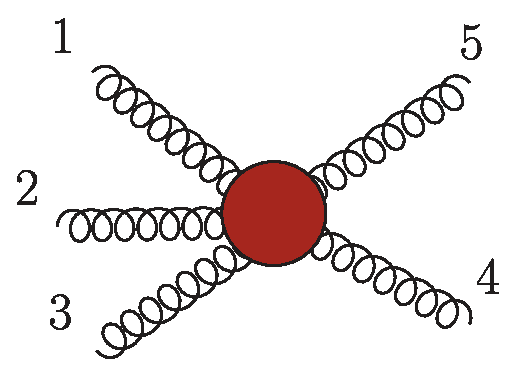
\includegraphics[height=\figureheight]{TreeFull}}} 
    \qquad \xrightarrow[p^2_\xi \to m_\xi^2]{} \quad
    \frac{1}{p^2_\xi - m_\xi^2} \cdot
    \sum_{i\in \text{states}}^{} ~
    \vcenter{\hbox{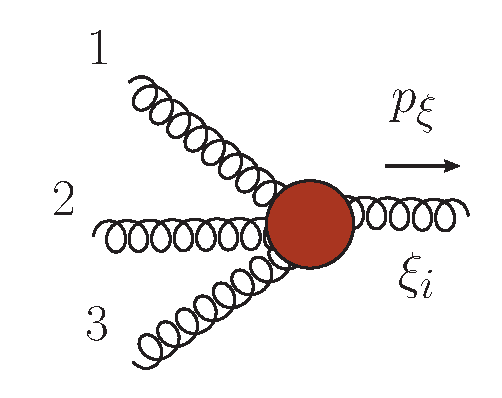
\includegraphics[height=0.9\figureheight]{TreeLeft}}}\cdot
    \vcenter{\hbox{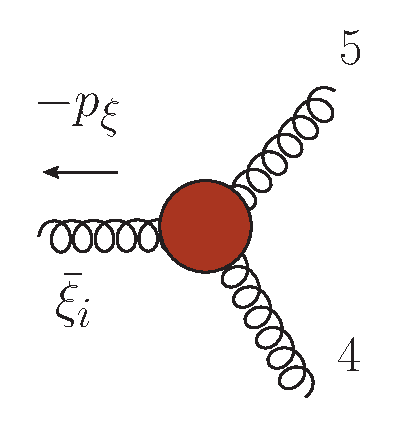
\includegraphics[height=0.9\figureheight]{TreeRight}}}
  \end{equation*}
  \caption{
    An example of factorization due to a physical pole singularity. 
    Here $p_\xi =  p_1 + p_2 + p_3$.
  }
  \label{fig:factorization}
\end{figure}


\todo{Note that in \cref{eq:optical_theorem} there is a phase-space integral present on the right-hand side}

The exact singularity as expected cannot be reached in any physical process.
However if we analytically continue an amplitude to complex external momenta,
it is possible to choose them to hit the pole explicitly
while still satisfying on-shell conditions for external states.


\subsection{On-Shell Recursion}
\label{sec:BCFW}

The universal factorization  property expressed by \cref{eq:factorization_pole} is independent of perturbation theory. 
For tree-level amplitudes however the factorization can be discovered rather straightforwardly by inspection,
although it might be obscured in the expressions found within the standard Feynman-diagrammatic approach.

The factorization of tree amplitudes can be converted into an algorithm to evaluate them.
This is done through the systematic exploration of the amplitude's factorization limits such that
it can be broken down recursively to sums of lower-multiplicity tree amplitudes. 
The building blocks of this recursion are thus on-shell amplitudes.
This idea is known as \emph{Britto-Cachazo-Feng-Witten} (BCFW) recursion \cite{Britto2005c,Britto2005f}.
The on-shell recursion is a very powerful tool for analytical computations, especially 
in theories with supersymmetry \cite{Dixon:2010ik,Drummond:2008cr,Bourjaily:2010wh}.
However for numerical applications and general models the on-shell recursion algorithm
does not offer benefits over off-shell alternatives, both in speed and numerical stability \cite{Duhr:2006iq,Drummond:2008cr,Badger:2012uz},
especially if one is interested in tree amplitudes in arbitrary number of space-time dimensions (see \cref{chap:numunitarity}). 


\subsection{Generalized Cuts}

Unitarity can be turned into a computational method of loop amplitudes as well.
A certain class of one-loop amplitudes, which
can be written as a sum of box, triangle, and bubble scalar integrals,
\begin{equation} \label{eq:cut_constructable_ampl}
  A^{(1)} = \sum_i d_{i}\,\vcenter{\hbox{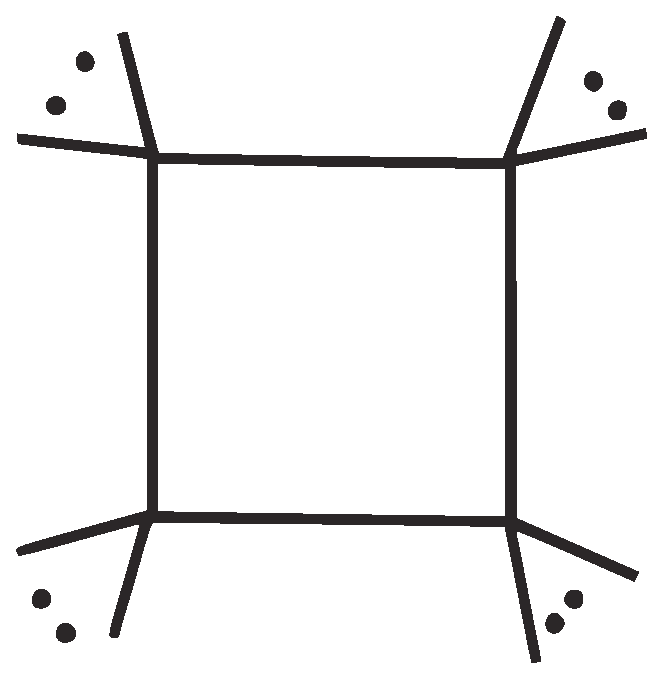
\includegraphics[width=8ex]{boxintegral}}}_i~+~
  \sum_{i}^{} c_{i}\,\vcenter{\hbox{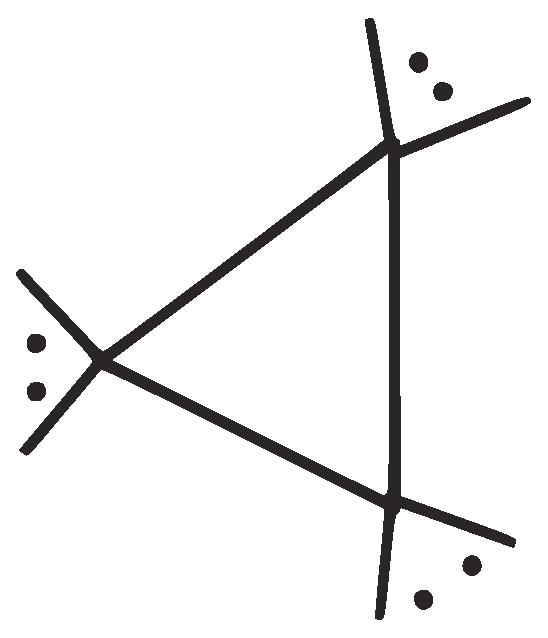
\includegraphics[width=7ex]{triangleint}}}_i~+~
  \sum_i b_{i}\,\vcenter{\hbox{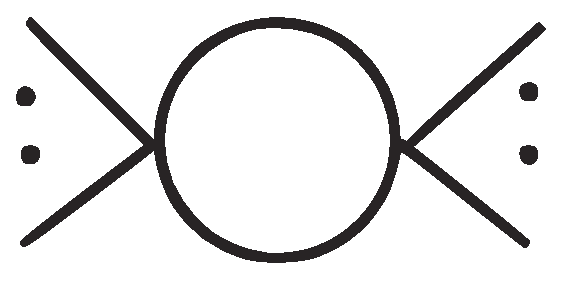
\includegraphics[width=8ex]{bubint}}}_i
\end{equation}
can be obtained entirely from unitarity cuts computed through Cutkosky rules \cite{Bern:1994cg,Bern:1994zx}.
Each integral in \cref{eq:cut_constructable_ampl} has unique discontinuities.
So the discontinuities of the loop amplitude on the left, 
evaluated as phase-space integrals over products of on-shell tree amplitudes as follows from unitarity,
can be matched to those of integrals to obtain equations for the integral coefficients.

However in general \emph{only} unitarity is not enough.

It is possible to generalize application of cuts given by \cref{eq:cut} to
obtain multi-channel discontinuities \cite{Britto:2004nc}.
For example see \cref{fig:quad_cut}.
Note that this kind of cuts are not direct consequences of unitarity of the $\mathcal{S}$-matrix (\cref{eq:unitarity_smatrix}), hence the name \emph{generalized} cuts.

\begin{figure}[ht]
  \centering
  \begin{equation*}
    \vcenter{\hbox{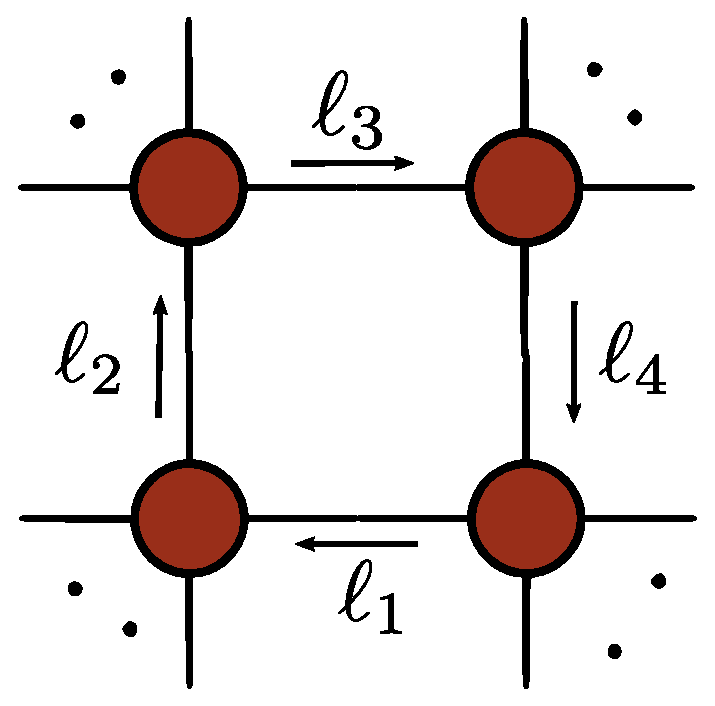
\includegraphics[width=0.2\linewidth]{box}}} \qquad \xrightarrow[i\in\{1\ldots4\}]{\ell_{i}^2-m_i^2\to~0} \qquad
    \vcenter{\hbox{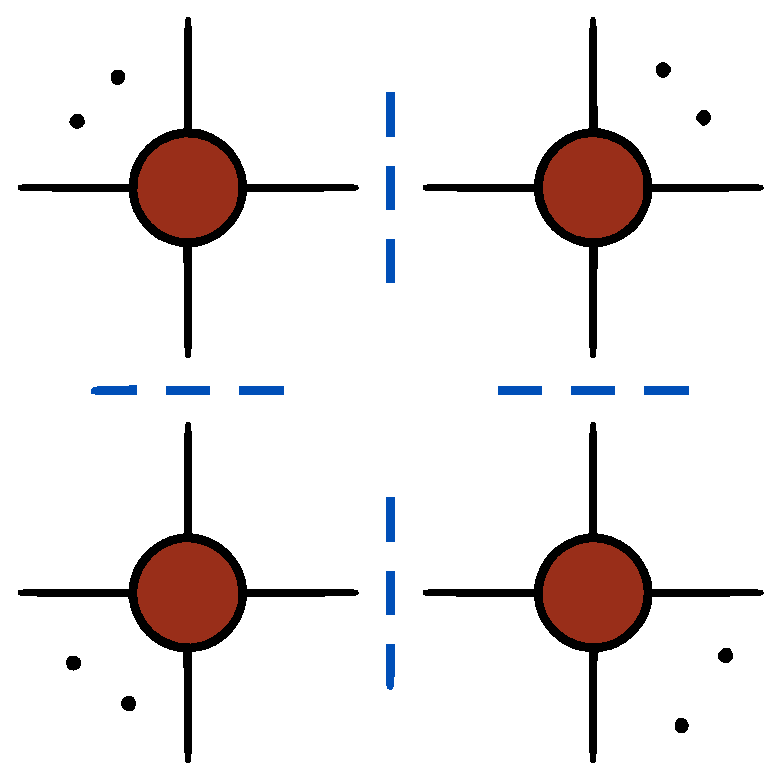
\includegraphics[width=0.2\linewidth]{boxCut}}}
    \quad = \quad \sum_{i}  c_{i} ~ m_{i}(\ell) %+ \sum_{i}  \tilde{c}_{i} \,\tilde{m}_{i}(\ell)
  \end{equation*}
  \caption{
    An example of a generalized cut.
    The loop momentum is chosen such that four propagator are simultaneously put to zero.
    On the left \emph{all} diagrams with the chosen propagators contribute.
    In the factorization limit each corner is a tree amplitude.
    The cut is matched to a basis of loop-momentum polynomials $\{m_i(\ell)\}$ on the right.
  }
  \label{fig:quad_cut}
\end{figure}


As a next step one can use the factorization of amplitudes on the cuts at the \emph{integrand} level  and match
it to a basis of loop-momentum polynomials in numerators (see \cref{fig:quad_cut}),
instead of integral coefficients \cite{Giele:2008ve,Ellis:2007br,Ellis:2008ir,Berger:2008sj}.
This matching procedure is intimately connected to a purely algebraical method of integral reduction known as OPP \cite{Ossola:2006us}.
This method uses the cut conditions \cref{eq:cut} to set some propagators to zero and triangularize linear systems for determining the basis coefficients.
It can be applied individually to each Feynman diagram or a sum thereof, thus having very little to do with factorization and unitarity.
When applied to the full amplitude however, it re

Somewhat confusingly sometimes generalized unitarity methods also refer 

Its flexibility allows for straightforward automation (see e.g.\ \cite{Berger:2008ag,Berger:2008sj,Cullen:2011ac,Mastrolia:2010nb,Ossola:2007ax}).

Most of the ideas mentioned in this section are formulated in the context of one-loop computations.
These give the first real taste of quantum nature of QFT.
Unfortunately, going beyond one-loop, many of the ideas do not generalize straightforwardly,
and require much more sophisticated computational techniques.
The extension of the ideas to multi-loop level have been actively studied in recent years \cite{Ita:2015tya,Abreu:2017idw,Abreu:2017hqn} 

In this thesis we apply the state-of-the-art developments for 


%%-------------------------------------------------

\chapter{Standard Techniques for Computation of Multi-Loop Amplitudes}
\label{chap:stdtech}
The aim of this chapter is brief overview of standard computational techniques for multi-loop amplitudes and
establishing the notation at the same time.

\section{Dimensional Regularization}



As we discussed in \cref{sec:hadcoll} loop amplitudes exhibit UV and IR divergences,
which must cancel in computations of any observable quantity.
However we have to regularize divergences at intermediate stages.
In principle any self-consistent regularization prescription should suffice.
However certain features of a regularization method such as breaking of Poincaré or gauge symmetries
can impact dramatically it's computational efficiency.
For this reason many different regularization schemes have been studied (for a recent review see \cite{Gnendiger:2017pys}).

In this thesis we regularize divergences by analytically continuing the dimensionality of space-time away from four to $D = 4 - 2\eps$ dimensions.
Divergences are then manifested in the no-regularization limit $D\to4$ (or $\eps\to0$) as poles in $\eps$.
This idea known as \emph{dimensional regularization} (DR) was introduced by 't Hooft and Veltman \cite{tHooft:1972tcz}.
Dimensional regularization has several advantages.
It explicitly preserves both Poincaré and non-chiral gauge symmetries.\footnote{\emph{chiral} gauge symmetries are in general violated by DR and require a special treatment}
Furthermore, it can be used as IR and UV regulator at the same time.
This makes it by far the most practical regularization scheme.


DR regularizes $L$-loop integrals by carrying out the integrations in $D$ dimensions, i.e. the integration measure is replaced as
\begin{equation}
  \int \prod_{i=1}^{L} \frac{\dd[4]{\ell_i}}{(2\pi)^{4}} ~\longrightarrow~ \quantity(\mu^{4-D})^{L}~\int \prod_{i=1}^{L} \frac{\dd[D]{\ell_i}}{(2\pi)^{D}}, \qquad \pdv{\ell^\mu_i}{\ell_{j\,\mu}} = \delta_{i j} D,
  \label{eq:dimregmeasure}
\end{equation}
where $\mu$ is an arbitrary mass scale to preserve the dimensionality of the coupling constants.

The fields and states transform as representations of Poincaré group,
implying that all Lorentz tensor and spinor structures (such as the metric tensor, momenta, external states, etc.) have
to be generalized to $D$ dimensions.
The are different flavors of DR making particular choices on how this generalization is accomplished (see e.g. \cite{Gnendiger:2017pys}).

The conceptually simplest variant of DR, the \emph{conventional dimensional regularization} (CDR)
treats all Lorentz structures uniformly in $D$ dimensions, effectively replacing the $SO(1,3)$ Lorentz symmetry by $SO(1,D-1)$.
CDR has been successfully employed in many analytic computations.
In this thesis however we are concerned with numerical methods, for which CDR is not very practical due to the
formally infinite number of external states.
Instead we use the 't Hooft -- Veltman (HV) scheme which keeps all external states and momenta in four dimensions and
extends the space-time symmetry group to $SO(1,3)\otimes SO(D-4)$.

It is advantageous to distinguish in the intermediate stages of computation the dimensionality of loop integration (or loop momenta) $D$ and
the dimensionality of internal particles $D_s > D$.
We will extensively exploit this separation in \cref{chap:dshel} to derive an efficient numerical numerical algorithm
for the evaluation of amplitudes in the HV scheme.
\todo{Consider removing the above phrase. It might be only needed in \cref{chap:dshel}}


\section{Loop Amplitudes}

For a particular choice of a gauge group, particle content, and operators of
a theory (which we collectively call a \emph{model}), Feynman rules can be derived.
Then the amplitudes in \cref{eq:amplitudes_expansion} can be obtained as a sum of all Feynman diagrams
with $N = 2+n$ specified external particles and $L$ loops.
For the purpose of this section we assume that the amplitudes $A^{L}_N$ are Lorentz-scalars.
This can be achieved for example by normalizing all amplitudes $A^{L}_N$ with $L\geq1$ by
a corresponding tree amplitude $A^{0}_N$ 
(see also \cref{chap:dshel,tab:results4parton1L,tab:results5parton1L,tab:results4parton,tab:results5parton}).


The most general form of any $L$-loop amplitude with $N$ external particles with momenta $p_1,\ldots,p_N$ and polarization states $\varepsilon_1,\ldots,\varepsilon_N$ is
\todo{clean up $\gamma$ sums in this section}
\begin{equation}
  \sum_{\Gamma \in \Delta} \qty(\int \prod_{i=1}^{L} \tilde{\dd{\ell_i}}) ~ \sum_{\gamma} 
  \frac{\mathcal{N}_{\Gamma,\gamma}%(\ell_1,\ldots,\ell_L,p_1,\ldots,p_{N-1})
    }{\prod_{j\in P_\Gamma} \rho_j^{\gamma_{j}}},
    \qquad \tilde{\dd{\ell_i}} \equiv \frac{\dd[D]{\ell_i}}{(2\pi)^{D}}.
  \label{eq:general_amplitude}
\end{equation}
Here $\rho_j = q_j^2 - m_j^2$ is a denominator of a propagator with momentum $q_j$ and mass $m_j$. The sum $\sum_{\gamma}$ runs over all possible assignments
of exponents $\gamma_{j} > 0$ of each propagator $\rho_j$. We define a \emph{topology} $\Gamma$ to be identified with a particular set of propagators $P_\Gamma$,
treating two sets of propagators equal if one can be transformed into the other with linear reparametrizations of loop momenta.
Note that topologies defined in this sense can have multiple graph representations.
The external sum runs over a set of all distinct topologies $\Delta$ contributing to the amplitude.
The numerators $\mathcal{N}_{\Gamma,\gamma_\Gamma}$
are functions of all possible scalar products of loop momenta, external momenta and polarization states.

Carrying out loop integrations in \cref{eq:general_amplitude} is extremely challenging task in general.
Fortunately there are many relations between integrals in \cref{eq:general_amplitude}.
And it is thus sufficient to consider a significantly smaller set of integrals $\Delta_\Gamma \subset \Delta$ commonly referred to
as \emph{master integrals}. Then the amplitude can be written in the form
\begin{equation}
  \sum_{\Gamma \in \Delta_\Gamma} \sum_{i\in M_\Gamma} ~ c_{\Gamma,i} ~ I_{\Gamma,i}, 
    \qquad I_{\Gamma,i} \equiv 
      \qty(\int \prod_{i=1}^{L} \tilde{\dd{\ell_i}}) \frac{m_{\Gamma,i}}{\prod_{j\in P_\Gamma} \rho_j^{\gamma_{i,j}}},
  \label{eq:amplitude_integrated}
\end{equation}
where $M_{\Gamma}$ is a set of particular choices of numerator insertions $m_{\Gamma,i}$ and exponents $\gamma_i$.
Despite the fact that the numerator functions $\mathcal{N}_{\Gamma,\gamma_\Gamma}$ in \cref{eq:general_amplitude} depend on the types of external particles and a particular model,
the master integrals $I_{\Gamma,i}$ are universal and determined only by kinematics.

Evaluation of amplitudes can thus be separated into two different problems:
\begin{enumerate}
  \item Extract the list of all relevant topologies and numerator insertions from \cref{eq:general_amplitude},
    identify master integrals and compute them.
  \item Reduce all terms in \cref{eq:general_amplitude} to the form of \cref{eq:amplitude_integrated}, thus
    determining the coefficients $c_{\Gamma,i}$.
\end{enumerate}
All process- and model-dependent information is contained in the master-integral coefficients $c_{\Gamma,i}$,
so the master integrals can be recycled for all kinematically-equivalent amplitudes.

In this thesis we focus on the reduction to master-integral coefficients.
We will review the standard approach in the next section, and
then explain how unitarity-based methods allow to address some of it's difficulties in \cref{chap:numunitarity}

\section{Classification of Numerators}
\label{sec:classification_numerators}

To solve the problem of reduction,
we need to classify all possible structures that can appear in the numerator functions $\mathcal{N}_{\Gamma,\gamma_\Gamma}$ in \cref{eq:general_amplitude}.

We start by making a convenient choice of independent variables.
Due to the Lorentz-invariance the numerators $\mathcal{N}_{\Gamma,\gamma_\Gamma}$ can only depend on scalar products
\begin{equation}
  \label{eq:sps_all}
  \vb*{sp} = \{ \sp(\ell_i,\ell_j),~\sp(\ell_i,p_j),~\sp(\ell_i, \tau_j) \}, \qquad \dim{\vb*{sp}} = D_{\text{ext}} L + \frac{1}{2}L(L+1),
\end{equation}
where $D_{\text{ext}}$ is the dimensionality of external states and momenta.
Here the vectors $\tau^i$ are the basis of the orthogonal complement of $\spn{p_1,\cdots,p_{N-1}}$ to the full four-dimensional Minkowski space,
so we have $p_i \cdot \tau_j = 0$.
The directions $\tau^i$ can be introduced to $\mathcal{N}_{\Gamma,\gamma_\Gamma}$ through external polarization states, hence
the scalar products $\sp(\ell_i, \tau_j)$ will drop out if polarization sums are performed.
In the HV scheme $D_{\text{ext}}=4$ and the number of corresponding scalar products is
\begin{equation}
  \label{eq:sp_counts}
  \renewcommand{\arraystretch}{1.5}
  \begin{tabular}[h]{p{10ex} p{20ex}}
    %$3N-10$ & $\sp(p_i,p_j)$ \\
       $\sp(\ell_i,\ell_j)$  &   $\dfrac{1}{2}L(L+1)$                \\
        $\sp(\ell_i,p_j)$    &   $\min\qty(4,N-1) ~L$                  \\
       $\sp(\ell_i, \tau_j)$ &   $ \qty\big(4-\min\qty(4,N-1)) L $  \\
  \end{tabular}
\end{equation}

The numerators $\mathcal{N}_{\Gamma,\gamma_\Gamma}$ can be thus represented as elements of a polynomial ring
$\mathcal{K}[\vb*{sp}]$ 
with coefficients $c_{\va{i}}(\vb*{x},D)$ being rational functions of external kinematics $\vb*{x}$ and $D$:
\begin{multline}
  \mathcal{N}_{\Gamma,\gamma_\Gamma}(\vb*{x}, \vb*{sp}, D) = \sum_{\va{i} : \abs{\va{i}} < H_{\Gamma}} c_{\va{i}} (\vb*{x},D)~ m^{\va{i}}(\vb*{sp}), \\
  m^{\va{i}}(\vb*{sp}) = (\sp(\ell_1,\ell_1))^{i_1} ~\cdots~ (\sp(\ell_1,p_1))^{i_{\min\qty(4,N-1)L}} ~\cdots~,
  %%(\sp(\ell_L, \tau_{4-\min\qty(4,N-1)}))^{\i_{\dim{\vb*{sp}}}}
\end{multline}
\todo{fix the monomial definition} 
where the sum runs over all monomials $m^{\va{i}}(\vb*{sp})$ with \emph{total degree} $\abs{\va{i}} \equiv \sum_j i_j$ less than
$ H_{\Gamma} $, which is determined by the UV structure of the model in consideration.


For a given topology $\Gamma$ in \cref{eq:general_amplitude} we chose $N_p$ denominators $\vb*{\rho}\equiv\{\rho_1,\ldots,\rho_{N_p}\}$ as
independent variables. Then $N_p$ scalar products from the set $\vb*{sp}$
can be expressed as functions of the denominators $\vb*{\rho}$.
This implies
that whenever these scalar products are encountered in $\mathcal{N}_{\Gamma,\gamma_\Gamma}\qty(\vb*{sp})$ they can be canceled with
one of the denominators and attributed to a topology with less propagators.
For this reason these scalar products are commonly called \emph{reducible scalar products} (RSP).
We choose the remaining scalar products
\begin{equation}
  \vb*{\alpha} \equiv \vb*{sp} \setminus \text{(RSP)}, \qquad \dim{\vb*{\alpha}} \equiv N_\text{ISP} =  \dim{\vb*{sp}}-N_p,
\end{equation}
which are called
\emph{irreducible scalar products} (ISP) to be the rest of our independent variables.

An important observation which becomes evident from our choice of variables is that all topologies with $N_p> 4 L +\frac{1}{2}L(L+1)$, no matter the number of external particles, are reducible.
Indeed in this case we have $(\dim\vb*{sp}) < N_p$ so there are no irreducible scalar products, and only $(\dim\vb*{sp})$ denominators can be independent.

\todo{potential include a relation which reduces product of more than $\dim\vb*{sp}$ propagators to $N_p$ propagators}

After a change of variables $\vb*{sp}\to \{\vb*{\rho},\vb*{\alpha}\}$ and cancellation of denominators
we find that the numerators are now polynomials in ISPs only:
\begin{equation}
  \label{eq:rsp_reduction}
  \mathcal{N}_{\Gamma,\gamma_\Gamma}(\vb*{x}, \vb*{sp}, D) \longrightarrow \qquad
    \mathcal{N}^{\prime}_{\Gamma,\gamma_\Gamma}(\vb*{x}, \vb*{\alpha}, D) =
    \sum_{\va{i} : \abs{\va{i}} < H_{\Gamma}} c^{\prime}_{\va{i}} (\vb*{x},D)~ m^{\va{i}}(\vb*{\alpha}),
\end{equation}
and all topologies with $N_p > 4L +\frac{1}{2}L(L+1)$ are eliminated.
In practice this can be non-trivial and systematically performed with Gröbner basis techniques \cite{Zhang:2012ce,Mastrolia:2012wf,Mastrolia:2012an,Mastrolia:2016dhn}.
In unitarity-based approaches this step is taken into an account by construction,
and need not be carried out explicitly. We discuss this in more detail in \cref{sec:ansatz_integrand}

For $L=1$ the only irreducible scalar products are of the transverse type $\sp(\ell_i, \tau_j)$, which vanish upon integration due to Lorentz symmetry either directly,
or after some simple considerations (see \cref{sec:traceless_completion} for details).
For $L>1$ however this is not the case and there are more identities which we can take advantage of to reduce the number of master integrals.
We discuss this in the next section.

\todo{mention 1-loop techniques: OPP and PV here somehow?}

We conclude this section with a remark that the variables $\{\vb*{\rho},\vb*{\alpha}\}$ we chose for parametrization of the integrand can be promoted
to the integration measure in \cref{eq:general_amplitude}. This representation of loop integrals known as the \emph{Baikov representation} \cite{Baikov:1996rk} 
makes $4 L +\frac{1}{2}L(L+1)$ non-trivial integrations manifest, and allows to trivially integrate out irrelevant loop-momenta directions. This representation
exhibits many other useful properties, nonetheless we will not need to adopt it in this thesis.


%We parametrize loop momenta as follows
%\begin{subequations}
  %\begin{equation}
    %\ell_l = \ell_{l[4]} + \ell_{l[D-4]}, \qquad 
    %\begin{array}[]{ll}
      %\ell^\mu_{l[4]} &\equiv g^{\mu\nu}_{[4]} \ell_\nu \\
      %\ell^\mu_{l[D-4]} &\equiv g^{\mu\nu}_{[D-4]} \ell_\nu \\
    %\end{array},
    %\qquad
    %\ell_{l[4]}\cdot\ell_{l[D-4]} = 0,
    %\label{eq:loop_momenta}
  %\end{equation}
  %and
  %\begin{align}
    %\ell_{l[4]} &=  \sum_{i\in \mathcal{B}_{\text{phys}}} c^{i}_l ~ v^{i} ~+~ \sum_{i\in \mathcal{M}_{[4]}\setminus\mathcal{B}_{\text{phys}}} \chi^{i}_l ~ \tau^i, \\ 
    %\ell_{l[D-4]} &=  \sum_{i\in\tilde{\mathcal{B}}} \mu^i_l ~ \tilde{n}^{i},
  %\end{align}
%\end{subequations}
%where $v^{i}$ are basis vectors of the vector space $\mathcal{B}_{\text{phys}} \equiv \spn{p_1,\cdots,p_{N-1}}$ spanned by $N-1$ external momenta;
%the vectors $\tau^i$ span the orthogonal complement of $\mathcal{B}_{\text{phys}}$ to the four-dimensional Minkowski space $\mathcal{M}_{[4]}$.


\section{Integration-by-Parts Identities}
\label{sec:ibp}


Using \cref{eq:rsp_reduction} we can bring \cref{eq:general_amplitude} to the form 
\begin{equation}
  \sum_{\Gamma \in \Delta} \sum_{\gamma} \sum_{\va{i}} ~ c_{\Gamma\gamma, \va{i}} (\vb*{x},D) ~ 
  \qty(\int \prod_{i=1}^{L} \tilde{\dd{\ell_i}}) ~  
  \frac{m^{\va{i}}_{\Gamma\gamma}(\vb*{\alpha})%(\ell_1,\ldots,\ell_L,p_1,\ldots,p_{N-1})
    }{\prod_{j\in P_\Gamma} \rho_j^{\gamma_{j}}}.
  \label{eq:rsp_reduced_amplitude}
\end{equation}
The integrals in \cref{eq:rsp_reduced_amplitude} are process-independent and have the desired form of \cref{eq:amplitude_integrated}.
However we are still missing a large number of identities due to the vanishing of the total derivative in dimensional regularization.
These identities are known as \emph{integration-by-parts} (IBP) identities \cite{Chetyrkin:1981qh,Tkachov:1981wb} and have a general
form of
\begin{equation}
  \qty(\int \prod_{i=1}^{L} \tilde{\dd{\ell_i}}) ~  \pdv{\ell_k^\mu}(
  \frac{ v_k^\mu \ommit{(\vb*{x},\vb*{\rho},\vb*{\alpha},D)} ~ \, m^{\va{i}}(\vb*{\alpha})
    }{\prod_{j} \rho_j^{\gamma_{j}}}
    ) = 0,
  \label{eq:ibps}
\end{equation}
where the components of \emph{IBP vectors} $v_k^\mu(\vb*{x},\vb*{\rho},\vb*{\alpha},D)$ are arbitrary rational functions
of all variables. The monomials $m^{\va{i}}(\vb*{\alpha})$ can be absorbed in $v_k^\mu$, but
it's convenient to keep them separate.

It is useful to organize all topologies $\Delta$ in \cref{eq:rsp_reduced_amplitude}
hierarchically by defining a partial ordering
\begin{equation} \label{eq:topology_order}
    \Gamma_1 > \Gamma_2 \iff P_{\Gamma_1} \supset P_{\Gamma_2},
\end{equation}
meaning that topology $\Gamma_2$ is obtained from topology $\Gamma_1$ by removing one or more propagators.
We then slice $\Delta$ into strictly ordered (overlapping) subsets $\Delta_i$ such that
\begin{subequations} \label{eq:topology_sequence}
    \begin{gather}
         \Delta = \bigcup_i \Delta_i,  \\
         \Delta_i  = \{\Gamma \in \Delta : \forall (\Gamma_1, \Gamma_2) \in\Delta \qif\qty( \Gamma_1 \in \Delta_i \qand \Gamma_2 < \Gamma_1) \qthen \Gamma_2 \in \Delta_i \}.
    \end{gather}
\end{subequations}
A subset $\Delta_i$ can thus be identified by it's ``greatest'' topology $\Gamma_{\Delta_i}$ ---
the topology with the maximal number of propagators, which we will call a \emph{parent} topology (or diagram).

If we allow exponents $\gamma_j$ in \cref{eq:rsp_reduced_amplitude} to be $\leq0$,
all integrals in \cref{eq:rsp_reduced_amplitude} can be cast into \emph{families}
\begin{equation} \label{eq:integral_families}
    I_{\Delta_i}[\va{\gamma},\va{i}] \equiv 
  \qty(\int \prod_{i=1}^{L} \tilde{\dd{\ell_i}}) ~  
  \frac{m^{\va{i}}_{\Gamma_{\Delta_i}}(\vb*{\alpha})%(\ell_1,\ldots,\ell_L,p_1,\ldots,p_{N-1})
    }{\prod_{j\in P_{\Gamma_{\Delta_i}}} \rho_j^{\gamma_{j}}}.
\end{equation}
IBP identities of \cref{eq:ibps} generate an under-determined system of homogeneous linear equations between integrals inside a family.
The integrals which cannot be determined from the system are chosen to be master integrals.
The remaining integrals are then expressed as linear combinations of master integrals.
A systematic approach of generating and solving a complete system of IBP identities was formulated by Laporta \cite{Laporta:2001dd}.
There are multiple publicly available implementations such as
\textsc{Reduze} \cite{Studerus:2009ye,vonManteuffel:2012np},
\textsc{Fire} \cite{Smirnov:2008iw,Smirnov:2014hma},
\textsc{LiteRed} \cite{Lee:2012cn,Lee:2013mka},
\textsc{Kira} \cite{Maierhoefer:2017hyi,Maierhofer:2018gpa}, etc.

The problem of IBP reduction is in general very difficult, which
is due the very large amount of relations produced from \cref{eq:ibps}, and
hence the requirement to solve large linear systems.
This is due to the number of choices of IBP vectors, as well as the fact that IBP identities
in general include the relations for integrals with denominators raised to powers larger than one, even
though this integrals are mostly not found from Feynman rules.

Although as for master integrals if solved, the reduction tables can be recycled, but fully analytic approaches cannot solve linear systems. 
And even if the reduction table tables can be produced, they are not usable in practice \cite{Chawdhry:2018awn}.

In \cref{chap:numunitarity} we discuss how this difficulty can be addressed by unitarity-based methods,
which do not require the solution of the full IBP system.

\todo{Example?}


\section{Master Integrals}

Once the set of master integrals is found, the IBP reduction relations can be applied 
to all terms in \cref{eq:rsp_reduced_amplitude}.
This determines the coefficients of master integrals
\begin{equation} \label{eq:master_integrals}
    \qquad I_{\Gamma,i} = 
    \qty(\int \prod_{i=1}^{L} \tilde{\dd{\ell_i}}) \frac{m_{\Gamma,i}}{\prod_{j\in P_\Gamma} \rho_j^{\gamma_{i,j}}}.
\end{equation}
in \cref{eq:amplitude_integrated}.

\todo{choice of masters: uniform weight, finite, unitarity compatible} 

A variety of methods have been developed for evaluation of the master integrals.
Broadly speaking they can be classified into analytic and numerical methods.

Direct integration using a convenient choice of integration variables is the most straightforward option.
All one-loop integrals can be obtained this way \cite{vanHameren:2010cp,Ellis:2007qk,tHooft:1978jhc,Denner:2010tr}.
But for multi-scale multi-loop integrals this becomes  cumbersome quickly  very.
Another method is the integration in the Mellin-Barnes  representation  \cite{Smirnov:1999gc,Tausk:1999vh,Dubovyk:2017cqw}, which
has been used to solve some two-loop integrals.
However the most commonly used and successful method is to obtain analytic results via
differential equations \cite{Kotikov:1990kg,Remiddi:1997ny,Gehrmann:1999as,Henn:2013pwa,Argeri:2007up,Henn:2014qga}.

On the numerical side, the commonly used general methods are sector decomposition \cite{Binoth:2000ps,Binoth:2003ak}
and numerical Mellin-Barnes representation \cite{Czakon:2005rk,Anastasiou:2005cb}.
See e.g. \cite{Freitas:2016sty} for a review.

Usually the knowledge of analytical expressions is preferable since it allows for better control over
precision and performance required for Monte-Carlo integration over external phase space. However
some notable NNLO QCD computations have been carried out with at least one of the integrals evaluated through numerical
methods \todo{references}.

In this thesis we will not consider evaluation of master integrals.
For the class of process we are interested in the analytic results are available in the literature.


\chapter{Multi-Loop $D$-Dimensional Numerical Unitarity}
\label{chap:numunitarity}
In \cref{chap:stdtech} we sketched how a generic loop amplitude \eqref{eq:general_amplitude} can be reduced
to a sum of master integrals \eqref{eq:amplitude_integrated} in two stages.
First all reducible numerators are maximally canceled against corresponding denominators.
And after that the remaining numerators are reduced with IBP identities.
We indicated that the former can be rather challenging in some cases,
and the latter is one of the main bottlenecks in computations of
multi-scale two-loop amplitudes.
In this chapter we introduce a generalization of one-loop integrand-level unitarity-based methods \cite{Ossola:2006us,Giele:2008ve,Ellis:2008ir}
to two loops, which offers an alternative path to reduction of amplitudes and addresses the mentioned bottlenecks in an elegant way.
The foundations of this approach have been laid out in works \cite{Ita:2015tya,Abreu:2017xsl,Abreu:2017hqn,Abreu:2017idw}.
Some related work can also be found in 
\cite{Mastrolia:2011pr,Badger:2012dp,Badger:2013gxa,Zhang:2012ce,Mastrolia:2013kca,Mastrolia:2016dhn,Mastrolia:2012an,Kleiss:2012yv,Feng:2012bm,Kosower:2011ty}.
Notably it is designed to be amenable for automation and efficient numerical implementation, which is indispensable
for addressing the problem of large expressions in multi-scale problems.

The approach we discuss in this chapter broadly speaking consists of two major ingredients.
This first is a special choice of integrand parametrization\footnote{sometimes also called \emph{ansatz}},
which we discuss in \cref{sec:ansatz_integrand}.
The second is exploiting integrand-level factorization limits of amplitudes originating from generalized unitarity (see \cref{sec:unitarity}),
which we discuss in \cref{sec:cut_equations}.


%Unlike many numerical implementations of  
%One of the important features is that we  

%Like in \cref{chap:stdtech}, here we will not refer to any particular model.
%We also postpone the discussion of helicity amplitudes until \cref{chap:dshel}
%and assume that

\todo{The computational methods described in this chapter are essential for obtaining the results we present in \cref{chap:wbb_pheno,chap:5parton}.}

\section{Master/Surface Integrand Parametrization}
\label{sec:ansatz_integrand}

We start by again considering a generic $L$-loop amplitude in \cref{eq:general_amplitude},
and  the classification of numerators from \cref{sec:classification_numerators}.
We organize all topologies hierarchically as described around \cref{eq:topology_order,eq:topology_sequence}.
but we \emph{do not} cast integrals into families by allowing exponents $\gamma_{\Gamma j}$ of propagators $\vb*{\rho}$ to be non-positive.

Instead we will construct a special basis of numerator functions for each topology independently,
\begin{equation} \label{eq:master_surface_basis}
  \mathcal{N}_{\Gamma \gamma_\Gamma} = \sum_{i \in M_{\Gamma\gamma_\Gamma} \cup S_{\Gamma\gamma_\Gamma}} c_{\Gamma\gamma_\Gamma, i}(\vb*{x},D) \; m_{\Gamma\gamma_\Gamma, i} (\vb*{x},D;\vb*{\rho},\vb*{\alpha}),
\end{equation}
where $S_{\Gamma\gamma_\Gamma}$ is a set of numerators which vanish upon integration, which we call \emph{surface terms}, $M_{\Gamma\gamma_\Gamma}$ is a set of numerators associated to master integrals.
Here we introduced a notation for distinguishing the arguments of $m_{\Gamma\gamma_\Gamma, i} (\vb*{x},D;\vb*{\rho},\vb*{\alpha})$,
which we will use throughout this chapter. 
It means that $m_{\Gamma\gamma_\Gamma, i}$ is a rational function of arguments on the left of ``;'', and \emph{polynomial} in the arguments on the right. 

We will refer to this basis as \emph{master/surface} basis or decomposition.
The advantage of having a master/surface basis is that
reducing an amplitude to it achieves
a complete reduction by construction,
and the coefficients $c_{\Gamma\gamma_\Gamma,i}$ for $i\in M_{\Gamma\gamma_\Gamma}$ are the coefficients
of master integrals in \cref{eq:amplitude_integrated}.
Also we do not need to consider topologies with $N_p > 4L + \frac{1}{2}L(L+1)$ since as we discussed in \cref{sec:classification_numerators}
they are reducible to topologies lower in the hierarchy.

Of course, this basis can be obtained from the standard approach of \cref{chap:stdtech}, which would not be a very illuminating exercise.
However the construction of master/surface decomposition can be cast into a much simpler computational problem than solving all IBP relations.
In what follows we review how this is accomplished.


\subsection{Transverse ISPs}
\label{sec:traceless_completion}

Consider a numerator $\mathcal{N}_{\Gamma\gamma_\Gamma}$ of a topology $\Gamma$ from $\Delta$ with $N_p <  4L + \frac{1}{2}L(L+1)$.
In this section we focus on one such numerator at a time, so we drop the topology labels.

What is meant by a set of numerator insertions $m_{i}(\vb*{x},D;\vb*{\rho},\vb*{\alpha})$ being a basis is that
$\spn{m_{i}}$ is equivalent
modulo RSPs (i.e.\ with the on-shell constraints $\rho_j = 0,\;\forall j\in P_\Gamma$ imposed)
as a linear vector space to a ring of polynomials $\mathbb{Q}_{\vb*{x},D}[\vb*{\alpha}]$.
Evidently how $m_{i}$ depend on $\vb*{\rho}$ is of no relevance for what concerns constructing
a basis in $\mathbb{Q}_{\vb*{x},D}[\vb*{\alpha}]$, but, as we will see shortly, sometimes the presence
of $\vb*{\rho}$ might be important for ensuring other features of $m_{i}$ such as vanishing
upon integration.

%\footnote{
  %more precisely: $\mathbb{Q}_{\vb*{x},D;\vb*{\rho}}[\vb*{\alpha}]$ has coefficients from a ring $\mathbb{Q}_{\vb*{x},D}[\vb*{\rho}]$,
  %which itself has coefficients from a field of rational functions $Q(\vb*{x},D)$
%}, 

It is convenient to start constructing the master/surface basis from a natural basis of monomials from $\mathbb{Q}_{\vb*{x},D}[\vb*{\alpha}]$:
\begin{equation}
  \mathcal{N} = \sum_{\va{i}}^{} c_{\va{i}}(\vb*{x},D;\vb*{\rho}) \; m^{\va{i}}(\vb*{\alpha}), \qquad
  m_\Gamma^{\va{i}}(\vb*{\alpha}) = \vb*{\alpha}^{\va{i}} \equiv 
  %\rho_1^{i_1}\,\ldots\,\rho_{N_p}^{i_{N_p}} ~
  %\alpha_1^{i_{N_p+1}}\,\ldots{}\,\alpha_{N_\text{ISP} }^{i_{N_p+1 +N_\text{ISP} }}.
  \alpha_1^{i_1}\,\ldots{}\,\alpha_{N_\text{ISP} }^{i_{N_\text{ISP} }}.
\end{equation}
where we allow coefficients $c_{i}$ to depend on $\vb*{\rho}$.
%except for $\eval{c_{\va{i}}}_{\rho_j \to 0} = 0$,
%such that all monomials  stay irreducible.
The basis of the linear vector space of all monomials from $\mathbb{Q}_{\vb*{x},D}[\vb*{\alpha}]$ is of course infinite,
but the maximal degree  we need to consider $\mathsf{P}$ in practice is always limited from above by UV behavior of the particular model under consideration.
The number of basis elements is thus 
\begin{equation} \label{eq:number_of_monomials}
  \dim{\spn{\vb*{\alpha}^{\va{i}} : \abs{\va{i}} \leq  \mathsf{P}}} =  \frac{(N_\text{ISP} + \mathsf{P})!}{N_\text{ISP}! \mathsf{P}!}.
\end{equation}

Recall that some of the scalar products from $\vb*{\alpha}$ have a form $\sp(\ell_i,\tau_j)$ with $\tau_j$ transverse to all external momenta $p_i$.
We will denote these as $\vb*{\alpha}^\tau$.
From Lorentz symmetry an $L$-loop integral of an arbitrary rational function $f(\vb*{\vb*{x},\vb*{\rho}},D)$ is
\begin{equation} \label{eq:rank_1_tensor_integral}
  \Dmeasure{}~ f(\vb*{\vb*{x},\vb*{\rho}},D) ~ \ell_k^{\mu} = \sum_{i}^{}c_i(\vb*{x},D)\;p^\mu_i.
\end{equation}
Contracting both sides with $\tau^\mu_j$ and using the orthogonality condition we obtain
\begin{equation}
  \Dmeasure{}~ f(\vb*{\vb*{x},\vb*{\rho}},D) ~ \alpha^{\tau}_{k j}( \equiv \sp(\ell_k,\tau_j)) \quad = 0.
\end{equation}
Following the same argument it is easy to see that all monomials $\vb*{\alpha}^{\va{i}}$ with at least
one of the transverse ISPs taken to an odd power are vanishing upon integration and thus can be taken as surface terms as is.

Next we consider a rank 2 tensor integral
\begin{equation}
  \Dmeasure{}~ f(\vb*{\vb*{x},\vb*{\rho}},D) ~ \ell_k^{\mu}\ell_k^{\nu} = c_0\,g^{\mu\nu}_{[D]} + \sum_{i,j}^{}c_{i,j}\;p^\mu_i p^\nu_j,
\end{equation}
where the arguments of all coefficient are as in \cref{eq:rank_1_tensor_integral}, and we explicitly specified the dimensions of the metric tensor.
Upon contraction with $g^{\mu\nu}_{[D-4]}$ or $\tau_j^\mu\tau_j^\nu$, and taking into an account
\[
  g^{\mu\nu}_{[D]}g^{\phantom{\mu\nu}}_{[D-4]\nu\mu} = D-4,
\]
only $c_0$ survives.
We can then easily find a combination of two contractions which make the right-hand side vanish. Applying it to the left-hand side, we have
\begin{equation}
  \qty(\tau_j^\mu\tau_j^\nu - \frac{g^{\mu\nu}_{[D-4]}}{D-4}) ~ \ell_k^{\mu}\ell_k^{\nu} = (\alpha_j^\tau)^2 - \frac{\mu_{kk}(\vb*{\rho},\vb*{\alpha})}{D-4} \longrightarrow 0,
\end{equation}
where $\mu_{kj} \equiv g^{\phantom{\mu\nu}}_{[D-4]\mu\nu} \ell_k^\mu \ell_j^\nu$, so the expression on the right is a surface term and
we append it to our basis.

Similar relations can be found for any product of even powers of $\alpha_j \in \vb*{\alpha}^\tau$.
They can all be generated with the projector \todo{is it a projector?} 
\begin{equation}
  \mathrm{P}^{\mu_1\ldots{}\mu_n}_j =  \tau^{\mu_i}_j\ldots{}\tau^{\mu_n}_j - \frac{1}{n}\frac{1}{D-4} \sum_{\sigma \in \mathcal{G}_{2;n}}^{} g^{\mu_{\sigma(1)}\mu_{\sigma(2)}}_{[D-4]}~\tau^{\mu_{\sigma(3)}}_j\ldots{}\tau^{\mu_{\sigma(n)}}_j,
\end{equation}
where the sum is over all inequivalent ways to distribute indices $\{\mu_1,\ldots{},\mu_n\}$ in the summand.
We will refer to such relations as \emph{traceless completions}.
Note that although $\mu_{kj}(\vb*{\rho},\vb*{\alpha})$ are partially reducible to lower topologies,
we cannot use their reduction $\mu_{kj}(0,\vb*{\alpha})$ in traceless completion. If we do use it, the
corresponding insertion will no longer be vanishing upon integration.
The same applies in general for all surface terms.

As an example, we list all traceless completions sufficient for the computation of two-loop amplitudes in renormalizable theories:
\begin{align} \label{eq:traceless_completion_replacements}
  (\alpha_{kj}^{\tau})^2 &\to (\alpha_{kj}^{\tau})^2 - \frac{\mu_{kk}}{D-4}, \\
  \nonumber
  (\alpha_{kj}^{\tau})^2(\alpha_{k^\prime j}^{\tau})^2 &\to
  (\alpha_{kj}^{\tau})^2(\alpha_{k^\prime j}^{\tau})^2 - \frac{1}{D-4} \qty(
    \frac{1}{2}(\alpha_{kj}^{\tau})^2 \mu_{k^\prime k^\prime} ~+~ \alpha_{kj}^{\tau}\alpha_{k^\prime j}^{\tau} \mu_{k k^\prime} + \frac{1}{2}(\alpha_{k^\prime j}^{\tau})^2 \mu_{k k}
  ).
\end{align}

To summarize, all transverse ISPs are either trivially surface terms or can be turned into surface terms with the replacements of \cref{eq:traceless_completion_replacements}.
After this is done we are left to consider monomials from the ring $\mathbb{Q}[\vb*{\alpha}\setminus\vb*{\alpha}^\tau]$ only.


We conclude this section with two remarks.
First, at one loop the master/surface decomposition is hereby complete since all ISPs are transverse.\footnote{%
  there is a peculiar exception, see examples in \cref{sec:ms_examples}
}
Second, the traceless completions of transverse ISPs alternatively
can be obtained through a specially constructed IBP identities \cite{Ita:2015tya}.

\todo{Note that propagator exponents are irrelevant for traceless completion} 

%vectors of the form
%\begin{equation}
  %v^\mu = (\sp(n_\epsilon^i,\ell))~\ell^\mu - (\sp(\tau,\ell))~n_\epsilon^{i\,\mu}
%\end{equation}


\subsection{Unitarity-Compatible IBP Identities}
\label{sec:unitarity_compatible_ibps}
So far our set of numerator insertions $m_{\Gamma,i}$ consists of monomials with odd powers of transverse ISPs and traceless-completions of
monomials with even powers of transverse ISPs, which are all surface terms.
This leaves us to consider the span of polynomial ring $\mathbb{Q}_{\vb*{x},D}[\hat{\vb*{\alpha}}\equiv \vb*{\alpha}\setminus\vb*{\alpha}^\tau]$,
%truncated by the imposed power counting condition,
which is the hardest part of the master/surface decomposition.

The reason why not all terms from $\mathbb{Q}_{\vb*{x},D}[\hat{\vb*{\alpha}}]$ are master terms is that they are
related through IBP identities \eqref{eq:ibps}. So what we need to do is
\begin{enumerate}
  \item Generate IBP identities which relate
    \emph{only} monomials from $\mathbb{Q}_{\vb*{x},D}[\hat{\vb*{\alpha}}]$, i.e.\ those which do not increase powers of denominators (and do not add new denominators).
    These identities can all be taken as surface terms, but they are not independent. 
    \label{item1}
  \item  Viewing each surface term as a vector in the linear space of monomials $\hat{\vb*{\alpha}}^{\va{i}}$, take
    a basis of this space as the set $\hat{S}_\Gamma$
    \label{item2}
  \item The vectors from the complement $\mathbb{Q}[\hat{\vb*{\alpha}}]\setminus \hat{S}_\Gamma$ are then master terms $M_\Gamma$
    \label{item3}
\end{enumerate}

In principle the described procedure can be carried out with standard IBP reduction techniques discussed in \cref{sec:ibp}.
However this would be rather wasteful
since the vast majority of IBP identities involve relations between different topologies and doubling of denominators.
And indeed currently publicly available reduction programs
\cite{Studerus:2009ye,vonManteuffel:2012np, Smirnov:2008iw,Smirnov:2014hma, Lee:2012cn,Lee:2013mka, Maierhoefer:2017hyi,Maierhofer:2018gpa}
have problems with reducing high degrees of ISPs in many variables.

Instead we can generate from the start only the IBP identities described in \cref{item1},
known as \emph{unitarity-compatible} IBP identities \cite{Gluza:2010ws,Schabinger:2011dz,Ita:2015tya}, by
restricting the IBP vectors $v_i^\mu$ in \cref{eq:ibps} to satisfy
\begin{equation} \label{eq:non_doubling_ibp_vectors}
  \sum_i v_i^\mu(\vb*{x},D;\vb*{\rho},\vb*{\alpha}) ~ \pdv{\ell^\mu_i} \rho_k = f(\vb*{x},D;\vb*{\rho},\vb*{\alpha}) ~ \rho_k, \qquad \forall k\in P_\Gamma,
\end{equation}
where it is crucial that both the arbitrary function $f$ and the vector components $v_i^\mu$ are polynomial in $\vb*{\rho}$ and $\vb*{\alpha}$, not rational.

{
  \def\coeff{c^{(\text{loop, ext})}_{ij,\va{k}_\rho \va{k}_{\hat{\alpha}}}}
  A naive way to find all vectors satisfying \cref{eq:non_doubling_ibp_vectors}
  is by inserting a simple ansatz
  \begin{equation} \label{eq:unitarity_compaible_ibp_ansatz}
    v_i^\mu = \sum_{j}^{}c^{(\text{loop})}_{ij}\ell^\mu_j ~+~  \sum_{j}^{}c^{(\text{ext})}_{ij} p^\mu_j, \qquad
    c_{ij}^{(\text{loop,ext})} = \sum_{\va{k}_\rho, \va{k}_{\hat{\alpha}}} \coeff (\vb*{x},D)\, \vb*{\rho}^{\va{k}_\rho}\vb*{\hat{\alpha}}^{\va{k}_\alpha}
  \end{equation}
  into \cref{eq:non_doubling_ibp_vectors}.
  The linear constraints for coefficients $\coeff$ can be then solved with standard linear algebra.
}%
In practice much more powerful methods of solving \cref{eq:non_doubling_ibp_vectors}  based on computational
algebraic geometry can be employed \cite{Larsen:2015ped,Boehm:2018fpv,Zhang:2016kfo,Abreu:2017xsl,Bendle2019}.

Having unitarity-compatible IBP vectors lets us trivially generate an overcomplete set of surface terms%
\footnote{
  It is worth noting that one has to be careful with power counting constraints at this stage.
  In general it is necessary to keep higher degree terms before eliminating linear dependences to get a complete set.
}
by inserting the vectors in \cref{eq:ibps}.
The spanning set (i.e.\ complete and non-redundant) is then obtained as outlined in \cref{item2,item3}.
The basis of numerators is constructed modulo RSPs, so
linear dependences between surface terms are found with on-shell conditions $\rho_j=0$ imposed.
This can be very helpful when the size of the basis gets large.
Another useful observation is that the surface terms obtained for a particular choice of exponents $\gamma_\Gamma$
of propagators from topology $\Gamma$ 
can be recycled for any other choice of exponents with minimal modifications.
Sometimes the set $M_\Gamma$ is found to be empty, which means that there are
no master integrals on this topology.


\todo{can be checked with standard IBP reduction} 


\subsection{Examples}
\label{sec:ms_examples}

We now consider some examples of constructing the master/surface basis.
First we take a look at all one-loop topologies, 
and then a two-loop topology.

\subsection{One-Loop Topologies}

Once a multi-loop generalization of the technology for finding master/surface decomposition 
is set up, the case $L=1$ seems to be nothing but a simple warm-up. 
Most of general features of the approach do in fact appear in one-loop topologies,
so it is instructive to consider.
Although, of course, the reader familiar with the one-loop literature may find
their application somewhat superfluous.

Compared to the ``usual'' basis of one-loop numerator insertions of \cite{Ossola:2006us,Giele:2008ve},
our basis will contain explicit $D$-dependence, and so will the coefficients.
This is the price paid for requiring to have the least amount of master integrals possible.
From efficiency perspective this is probably not a good idea for NLO computations,
since the terms of $\mathcal{O}(\epsilon)$ can be dropped
and extra master integrals can be arranged to be trivial, generating a so-called rational part.
For NNLO computations and beyond, where higher orders in the $\epsilon$-expansion are required, 
this might be not unreasonable to think of.

For $L=1$ the total number of scalar products is $\dim{\vb*{sp}} = 4\cdot 1+ 1 = 5$.
Hence topologies with the number of propagators $N_p>5$ are reducible.

%\begin{table}[ht!]
  %\centering
  %\begin{tabular}{cccccc}
    %\toprule
    %$N_p$ & $N_\text{ISP}$ & $\mathsf{P}$ & $\dim \spn{\vb*{\alpha}^{\va{i}}}$ & Monomials \\
    %5 & 0 & 5 & 1   &   $\{1\}$\\
    %4 & 1 & 4 & 5   & $\{1,\alpha_1,\alpha_1^2,\alpha_1^3,\alpha_1^4\}$\\
    %3 & 2 & 3 & 10  & \\
    %2 & 3 & 2 & 10  & $\{1,\alpha_1,\alpha_2,\alpha_3,\alpha_1^2,\alpha_1\alpha_2,\alpha_1\alpha_3,\alpha_2^2,\alpha_2\alpha_3, \alpha_3^2\} $ \\
    %1 & 4 & 1 & 5   \\
    %\midrule
    %\bottomrule
  %\end{tabular}
  %\caption{One-loop topologies}
  %\label{tab:counting_1l_topos}
%\end{table}

\textbf{Pentagon}

For pentagon topologies the 5 propagators $\{\rho_1,\ldots{}\rho_5\}$ are chosen as 5 independent variables,
so there are no irreducible insertions except for the scalar, and there are no IBP identities involving it. 
The one master insertion is usually chosen to be $\mu^2$, such that
the corresponding integral contributes only from  $\order{\epsilon}$.

\todo{Recall that $\mu^2(\vb*{\rho})$ is not an independent variable.} 

\textbf{Box}

For boxes we have  4 propagators $\{\rho_1,\ldots{}\rho_4\}$ and an ISP $ \alpha_1 = \sp(\ell,\tau_1), $
corresponding to one transverse direction.
The possible monomials up to degree 4 are 
\[
  \{1,~\alpha_1,~\alpha_1^2,~\alpha_1^3,~\alpha_1^4\},~
\]
from which $\alpha_1,\alpha_1^3$ are surface terms trivially.
For monomials $\alpha_1^2$ and $\alpha_1^4$ we use the traceless completions in
\cref{eq:traceless_completion_replacements}. There are no IBP relations for box topologies so
our master/surface decomposition is
\[
  M_{\Gamma_\text{box} } = \{1\}, \qquad S_{\Gamma_\text{box} } = \{\alpha_1,~ \alpha_1^2 - \frac{\mu^2}{D-4},~ \alpha_1^3,~ \alpha_1^4 - 3 \frac{\alpha_1^2~\mu^2}{D-4}\}.
\]
Compared to the ``standard'' choice (e.g.\ from \cite{Giele:2008ve}),
\[
  M_{\Gamma_\text{box} } = \{1, \mu^2, \mu^4\}, \qquad S_{\Gamma_\text{box} } = \{\alpha_1,~ \alpha_1 \mu^2 \}.
\]
we have two less master integrals.



\textbf{Triangle}

For triangles there are two ISPs: $ \alpha_1 = \sp(\ell,\tau_1)$, and $\alpha_2 = \sp(\ell,\tau_2)$,
corresponding to two transverse direction.
The 10 possible monomials up to total degree 3 are:
\[
\{1,~\alpha_1,~\alpha_2,~\alpha_1^2,~\alpha_1\alpha_2,~\alpha_2^2,~ \alpha_1^3,~ \alpha_1^2\alpha_2,~ \alpha_1\alpha_2^2,~ \alpha_2^3\}.
\]
from which all except $\{1,~\alpha_1^2,~\alpha_2^2\}$ are trivial surface terms,
and the last two are traceless completed.
For boxes and pentagons our considerations did not depend on a particular kinematics configuration.
For triangles this is not the case. For generic kinematics with massive propagators
and all $p_i^2\neq 0$, the decomposition is 
\begin{align*}
  M_{\Gamma_\text{tri} } &= \{1\}, \\
   S_{\Gamma_\text{tri} } &= 
  \{\alpha_1,~\alpha_2,~\alpha_1^2 - \frac{\mu^2}{D-4},~\alpha_1\alpha_2,~\alpha_2^2- \frac{\mu^2}{D-4},~ \alpha_1^3,~ \alpha_1^2\alpha_2,~ \alpha_1\alpha_2^2,~ \alpha_2^3\}.
\end{align*}
However for a special case when
\begin{equation}
  \begin{tabular}{ll}
    $\rho_1 = \ell^2$,               &  $p_1^2=0 \qor p_1^2\neq 0$, \\
    $\rho_2 = (\ell-p_1)^2$,         &  $p_2^2=0$,  \\
    $\rho_3 = (\ell-p_1-p_2)^2$, \hspace{2cm}    & $p_3^2\neq 0$, \\
  \end{tabular}
\end{equation}
we find non-trivial unitarity-compatible IBP vectors from \cref{eq:non_doubling_ibp_vectors}, for example
\[
  (\sp(p_1,p_2) + \rho_2 - \rho_3)~\ell^\mu  - \frac{1}{2} (2 \sp(p_1,p_2) + \rho_2 - \rho_3)~p_1^\mu  + \frac{1}{2}   (p_1^2 - \rho_1 - \rho_2)~p_2^\mu.
\]
Inserting it in \cref{eq:ibps} we obtain a surface term
\[  
  (D-4) \sp(p_1,p_2) + (D-3) (\rho_2-\rho_3).
\]
So for this kinematics configuration the whole space is spanned by surface terms,
\begin{align*}
  M_{\Gamma_\text{tri} } &= \{\}, \\
   S_{\Gamma_\text{tri} } &= 
  \Big\{(D-4) \sp(p_1,p_2) + (D-3) (\rho_2-\rho_3),\\ 
    &\qquad \alpha_1,~\alpha_2,~\alpha_1^2 - \frac{\mu^2}{D-4},~\alpha_1\alpha_2,~\alpha_2^2- \frac{\mu^2}{D-4},~ \alpha_1^3,~ \alpha_1^2\alpha_2,~ \alpha_1\alpha_2^2,~ \alpha_2^3 \Big\}.
\end{align*}
This happens very frequently starting from two loops.


\textbf{Bubble}

For generic kinematics we have 3 ISPs, $\{\alpha_1,~\alpha_2,~\alpha_3\}$, and
10 monomials up to the total degree 2,
\[
  \{1,~\alpha_1,~\alpha_2,~\alpha_3,~\alpha_1^2,~\alpha_1\alpha_2,~\alpha_1\alpha_3,~\alpha_2^2,~\alpha_2\alpha_3,~ \alpha_3^2\}.
\]
As before we convert all transverse ISPs to surface terms and we are left with one master integral.

There is an exceptional kinematical configuration,
\begin{equation*}
  \begin{tabular}{ll}
    $\rho_1 = \ell^2-m^2$,               &  \qquad $p_1^2=0$,\\
    $\rho_2 = (\ell-p_1)^2-m^2$,         &  \\
  \end{tabular}
\end{equation*}
for which something peculiar happens:
because $p_1$ is light-like, the transverse ``complement'' to it has to contain $p_1$ itself, thus the full four-dimensional space
cannot be decomposed into a direct sum of $\spn{p_1}$ and it's transverse, like we have done before.
Instead we have to introduce a random light-like vector $\tau_\chi^\mu$,
\[
  \tau_\chi^2=0, \qquad \sp(\tau_\chi,\tau_{\{1,2\}}) = 0, \qquad  \sp(p_1,\tau_\chi) \neq 0,
\]
such that $\spn{p_1,\tau_1,\tau_2,\tau_\chi}$ spans the full four-dimensional space.
We realize that $\chi \equiv \sp(\ell,\tau_\chi)$ is neither RSP nor it is a transverse ISP, so 
we need to employ IBP identities.
We add to the ansatz \eqref{eq:unitarity_compaible_ibp_ansatz} terms proportional to $\tau_\chi^\mu$ and solve them.
We find two surface terms,
\begin{align*}
  s_1 &= (\sp(p_1,\tau_\chi)) \qty(2 m^2 + \rho_1) - (D-1)\rho_1\chi, \\
  s_2 &= (\sp(p_1,\tau_\chi))^2 - 3 \chi^2,
\end{align*}
and can choose $\chi$ as the one master. The master/surface decomposition is thus
\begin{align*}
  M_{\Gamma_\text{b0} } &= \{\chi\}, \\
   S_{\Gamma_\text{b0} } &= 
  \{s_1,~s_2,~\alpha_1,~\alpha_2,~\alpha_1^2 - \frac{\mu^2}{D-4},~\alpha_1\alpha_2,~ \alpha_1\chi,~\alpha_2^2-\frac{\mu^2}{D-4},~\alpha_2\chi \}.
\end{align*}
Of course in this case the master integrals from insertions $\chi$ and $\chi^2$ can be computed trivially by direct integration.
For $m^2=0$ the corresponding integrals are scaleless, and vanish in dimensional regularization,
so this topology can be discarded.

\textbf{Tadpole}
Massless tadpoles vanish in dimensional regularization and can be discarded.
For massive tadpoles there are 4 transverse ISPs, and one master integral,
so the decomposition is done in the same way as above.

\subsection{Two-Loop Sunrise}

\begin{wrapfigure}{l}{0.25\linewidth}
  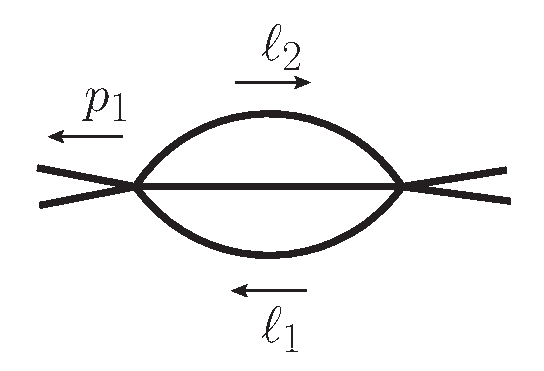
\includegraphics[width=1\linewidth]{sunrise_kinmatics_example}
\end{wrapfigure}
As a two-loop example we choose a two-loop massless ``sunrise'' topology, which is simple enough to fit the answer on a page.
For $L=2$ we have 11 scalar products. There are 3 propagators in the sunrise, so we have 8 ISPs in total.
From them 6 are transverse. 
We choose the independent variables to be 
\begin{align*}
  \rho_1 &= \ell_1^2,            \qquad & \alpha_1 = 2 (\sp(\ell_1,p_1)), \\
  \rho_2 &= \ell_2^2,                    & \alpha_2 = 2 (\sp(\ell_2,p_1)), \\
  \rho_3 &= (\ell_1-\ell_2-p_1)^2. &
\end{align*}
Using the formula \cref{eq:number_of_monomials} we get that there are 45 monomials up to the total degree 2.
39 of them contain at least one of the transverse ISPs, so we traceless complete them as in the one-loop case.
We are then left to deal with 6 monomials
\[
  \{1,~ \alpha_1,~ \alpha_2,~\alpha_1^2,~\alpha_1\alpha_2,~\alpha_2^2\}.
\]
Employing the ansatz \eqref{eq:unitarity_compaible_ibp_ansatz} we find lots of unitarity-compatible IBP vectors.
A couple of examples are:
\begin{equation*}
  \begin{tabular}{CC}
    v_1^\mu & v_2^\mu \\
    \midrule
    ( s -\alpha_2)\qty(( s  - \alpha_1) \ell_1^\mu + \rho_1 p_1^\mu)  &   (\alpha_2- s ) \qty( ( s +\alpha_2^2)\ell_2^\mu - \rho_2 p_1^\mu) \\
    (\alpha_1- s )\ell_1^\mu - \rho_1 p_1^\mu         &     ( s +\alpha_2) \ell_2^\mu - \rho_2 p_1^\mu \\
    \left( 2 s  - 2\alpha_1+\alpha_2 \right) \ell_1^\mu + \left( - s +\alpha_1-\alpha_2 + \rho_1 -\rho_2+\rho_3 \right) +\alpha_1\ell_2^\mu &  0\\
    \ldots{} & \ldots{}\\
    %\multicolumn{2}{C}{\ldots{}\ldots{}} \\
  \end{tabular},
\end{equation*}
where $s\equiv p_1^2$.
We use all these vectors to obtain the corresponding surface terms. 
In the next step we find the spanning set.
To do this we treat each surface term as a vector from the vector space 
$\spn{1,~ \alpha_1,~ \alpha_2,~\alpha_1^2,~\alpha_1\alpha_2,~\alpha_2^2}$,
and find a basis of the subspace spanned by all surface terms. 
It is important that we do this modulo RSPs, i.e.\ (temporarily) set $\rho_j\to 0$.
In this case we find that 5 of them are independent:
\begin{equation*}
  \small
  \begin{array}{l|l}
    s_1 & \alpha _1^2 (1-D)+\alpha _2^2 (-1+D)+s \left(\rho _1-2 \rho _2+\rho _3\right) \\
    s_2 & \alpha _1^2 (-3 (-1+D) (-4+3 D))+s \left(4 (-1+D)^2 s+3 (-4+3 D) \rho _1-6 (-2+D) \rho _2+3 (-4+3 D) \rho _3\right) \\
    s_3 & \alpha _1^2 ((-1+D) (-3+2 D))+\alpha _2 \alpha _1 \left(2 (-1+D)^2\right)+s \left((3-2 D) \rho _1-2 \rho _2+(3-2 D) \rho _3\right) \\
    s_4 & \alpha _1^2 (-4+(7-3 D) D)+\alpha _1 \left(2 (-1+D)^2 s\right)+s \left((-4+3 D) \rho _1-2 (-2+D) \rho _2+(-4+3 D) \rho _3\right) \\
    s_5 & \alpha _1^2 ((-1+D) (-4+3 D))+\alpha _2 \left(2 (-1+D)^2 s\right)+s \left((4-3 D) \rho _1+2 (-2+D) \rho _2+(4-3 D) \rho _3\right) \\
  \end{array}
\end{equation*}
This leaves us with just one master integral, which
we can choose to be any insertion linear independent from $\spn{s_1,\ldots{},s_5}$.
For example it can be the scalar integral.



\todo{Maybe also add an example for factorizable} 
%\subsection{Factorizable Topologies}

%We construct parametrization as 1-loop squared.
%Thus exactly as in 1-loop we find that all topologies with triangles
%with 1 or 2 external masses do not have masters and the surface term can be taken exactly the same as from 1-loop triangle.
%All other have exactly one master and otherwise the space is spanned by traceless completions.


\todo{Put somewhere: Starting from two loops will have $D$-dependence in the numerator from IBP identities, so
we can choose to abandon all-together the idea of not having it there.}

\section{Cut Equations}
\label{sec:cut_equations}
{

In the previous section we discussed how to construct a master/surface basis
of all possible numerators for each topology, so the integrand of an amplitude must 
be reducible to the form
\begin{equation} \label{eq:unitarity_ansatz}
  A^{(L)}(\{p_i,\varepsilon_i\}, \{\ell_k\}, D) \longrightarrow  
  \sum_{\Gamma \in \Delta} \sum_{\gamma_\Gamma} \sum_{i \in M_{\Gamma\gamma_\Gamma} \cup S_{\Gamma\gamma_\Gamma}} c_{\Gamma\gamma_\Gamma, i}(\vb*{x},D) \;
  \frac{m_{\Gamma\gamma_\Gamma, i} (\vb*{x},D;\vb*{\rho},\vb*{\alpha}) }%
    {\prod_{j\in P_\Gamma} \rho_j^{\gamma_{\Gamma i, j}}},
\end{equation}
whatever the initial representation of the amplitude on the left-hand side is.
For example it can be obtained as a sum of all Feynman diagrams.
The only thing left to compute the amplitude is then
to extract the coefficients $c_{\Gamma\gamma_\Gamma, i}$.
In principle we could sample the expression on the left-hand side with sufficient number of loop momenta,
and get a linear system of equations for $c_{\Gamma\gamma_\Gamma, i}$ by matching it to our ansatz on the right hand side.
But the system obtained this way would be so humongous that even a numerical solution would be problematic,
not to mention that evaluating the left hand side is usually not cheap either.

\def\gleading{{\gamma^{\textit{(l)}}_{\Gamma}}}
Fortunately the insights from generalized unitarity (see \cref{sec:unitarity}) suggest
a physics-motivated way of block-triangularizing the linear system for the coefficients $c_{\Gamma\gamma_\Gamma, i}$.
If we pick a topology $\Gamma$ and arrange loop momenta to satisfy it's on-shell limit $\rho_j \to 0,\;\forall j\in P_\Gamma$ (i.e.\ perform a cut),
the coefficients $c_{\Gamma\gleading,i}$ of the leading term in this limit
can be obtained through \emph{cut equations},
\begin{multline} \label{eq:cut_equations}
  \lim_{\ell^{\phantom{\Gamma}}_l \to \ell_l^{\Gamma}}\qty\Big( A^{(L)} \; {\prod_{j\in P_\Gamma} \rho_j^{\qty(\gleading)_j}} ) =  \\
  %
  \sum_i c_{\Gamma\gleading, i} ~ m_{\Gamma\gleading, i} \quad + \quad 
  %
  \sum_{\Gamma^\prime > \Gamma} \sum_{\gamma_{\Gamma^\prime}, i} 
  c_{\Gamma^\prime\gamma_{\Gamma^\prime}, i} \;
  \frac{m_{\Gamma^\prime\gamma_{\Gamma^\prime}, i}}{\displaystyle \prod_{j\in P_{\Gamma^\prime} \setminus P_\Gamma} \rho_j^{\gamma_{\Gamma^\prime i, j}}},
\end{multline}
which are \cref{eq:unitarity_ansatz} with terms of $\order{\rho_j^{\qty(\gleading)_j}}$ dropped, so
the sum $\sum_{\Gamma^\prime > \Gamma}$ is over topologies with more propagators 
(recall the organization into hierarchies by \cref{eq:topology_order,eq:topology_sequence}).
The cut equations are valid only for loop momenta $\ell_l^{\Gamma}$ that satisfy the cut conditions,
which we should take into an account when choosing sample values to generate the linear systems. 
In this way, going from the top of the hierarchy to the bottom
we solve cut equations one topology at a time, recycling the coefficients obtained earlier, effectively making the initial system block-triangular.

What is even better is that the left-hand side of \cref{eq:cut_equations} in the on-shell limit
can be evaluated as products of on-shell tree amplitudes,
\begin{equation} \label{eq:cut_amplitude}
    \lim_{\ell^{\phantom{\Gamma}}_l \to \ell_l^{\Gamma}}\qty\Big( A^{(L)} \; {\prod_{j\in P_\Gamma} \rho_j^{\qty(\gleading)_j}} ) \longrightarrow 
      \sum_{\text{states}} ~ \prod_{i \in T_\Gamma} A^{(0)}_i(\ell_l^{\Gamma},D),
\end{equation}
where the sum is over all states in $D$ dimensions, and $T_\Gamma$ corresponds to
all vertices of the topology $\Gamma$. The fact that this factorization takes place
at the level of \emph{integrand} is closely related but does not directly follow from generalized unitarity.
In practice the factorization can be rather straightforwardly realized by noticing the following \cite{Eden:1966dnq}: 
if one collects together all Feynman diagrams contributing to a particular topology,
each vertex of this topology is a sum of all tree graphs with fixed external legs,
hence it can be nothing else than a tree amplitude.
For an explicit example of how this happens see \cref{fig:example_factorization}. 
A notable exception to this observation can be found in the models which
contain non-trivial wave-function and mass renormalization for some of its' particles,
i.e.\ when there are non-vanishing one-particle-reducible diagrams \cite{Ellis:2008ir,Ellis:2011cr}.
These Feynman diagrams are absorbed into renormalization and have to be discarded from amplitudes by hand (\todo{see figure .}), hence
the vertices of the cut topologies to which they would contribute are \emph{not} tree amplitudes.
There is an interesting proposal to work around this issue \cite{Badger:2017gta}.
In practice however\footnote{%
  in this thesis we do not aim to follow the philosophy of ``never going off-shell'',
  but rather opt for whichever solution deemed more practical
}
it does not prevent us from using cut equations, but rather
demands some additional booking-keeping.

\begin{figure}[ht]
  \[
    \setlength{\figureheight}{0.07\textheight}
    \mathfigure{height=\figureheight}{example_tree_corner/f1} + 
    \mathfigure{height=\figureheight}{example_tree_corner/f2} + 
    \mathfigure{height=\figureheight}{example_tree_corner/f3}+ 
    \mathfigure{height=\figureheight}{example_tree_corner/f4} \longrightarrow 
    \mathfigure{height=1.5\figureheight}{example_tree_corner/corner}
  \]
  \caption{An illustration of diagrammatic ``proof'' of factorization. 
    On the left we show all Feynman diagrams contributing to a four-point one-loop amplitude of any theory with 3- and 4-point vertices
    in the channel $\{\ell^2,(\ell-p_1)^2,(\ell-p_1-p_2)^2\}\to 0$ given by the topology on the right.
    The tree amplitudes in the corners of the topology are assembled explicitly.
  } 
  \label{fig:example_factorization}
\end{figure}

Let us now mention how do we handle
the cases when the set of choices of propagators' exponents for some topology $\Gamma$
contains more than one element, that is there are propagators raised to powers greater than 1 \cite{Abreu:2017idw}.
As we mentioned above, the \cref{eq:cut_equations} directly isolates coefficients of 
the propagator structure with maximal total degree $\gleading$. For this propagator structure
also the factorization of \cref{eq:cut_amplitude} applies.
The coefficients of all the remaining propagator structures can be obtained together with the (leading) coefficients  of a topology one level below
$\Gamma$ in the hierarchy by ``undoing'' the block-triangularization.
Consider an example in \cref{fig:example_subleading_pole}.
The two-loop bubble-hexagon topology $\Gamma_1$ is given by a list of propagators $\{\rho_1,\ldots{},\rho_6\}$ and there are two
possible sets of exponents,
\[
  \Gamma_1 \leftrightarrow  \{\rho_1,\ldots{},\rho_6\}, \qquad \gamma_{\Gamma_1} =  
  \begin{pmatrix} 
    \{1,1,1,2,1,1\} &\leftarrow \gamma_{{\Gamma_1},1}  & \equiv \gamma_{\Gamma_1}^{(\textit{l})} \\ 
    \{1,1,1,1,1,1\} &\leftarrow \gamma_{{\Gamma_1},2} &
  \end{pmatrix}
\]
First we solve the cut equations for coefficients of $\gamma_{{\Gamma_1},1}$, and proceed down the hierarchy normally until we reach
the bubble-box topology $\Gamma_2$, not considering equations for the coefficients $\gamma_{{\Gamma_1},2}$.
We obtain the latter through the cut equations for $\Gamma_2$, treating them as unknowns together with 
the coefficients of the topology $\Gamma_2$ itself. Clearly this ``trick'' can always be performed
notwithstanding how many doubled (or tripled, etc.\@) propagators we encounter.
The only cost is that of solving the equations for larger number of coefficients.

Another possibility is to realize that the only cases when propagators can be raised to higher powers 
are from self-energy insertions on internal lines, which are associated to renormalization.
It turns out \cite{Baumeister:2019rmh} that
it is possible to cook up \emph{integrand-level} UV counter-terms such that
the integrand of the amplitude gets renormalized,
and all subleading poles vanish as a consequence.

We opt for the former approach as a simpler generic solution in favor of the
more intricate case-by-case study of the latter.
We observe that at least for two-loop
amplitudes a slight increase of ranks for some of the cut equations does not
pose any significant problem.

\todo{reference how to solve the equations} 

\begin{figure}[ht] 
  \centering
  \begin{tikzpicture}[scale=3,line width=1pt]
    \setlength{\figureheight}{0.08\textheight}
        % Maximal
    \node at (0,2){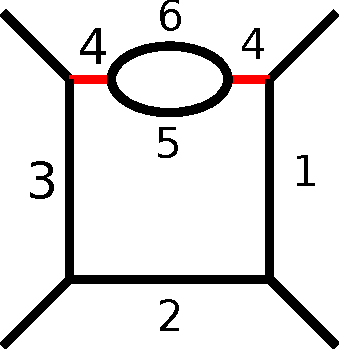
\includegraphics[width=\figureheight]{diagrams_from_4gluon/HexaBubbleThin}};
    \node at (0,1.5){ $\Gamma_1^{\{1,1,1,2,1,1\}}$}; 
    \node at (1,2){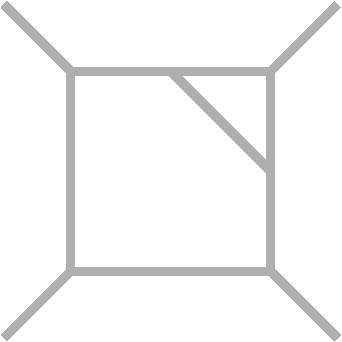
\includegraphics[width=\figureheight]{diagrams_from_4gluon/PentaTriangleThin}};
    \node at (2,2){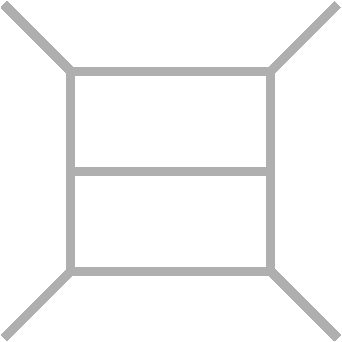
\includegraphics[width=\figureheight]{diagrams_from_4gluon/DoubleBoxThin}};
    \node at (3,2){\reflectbox{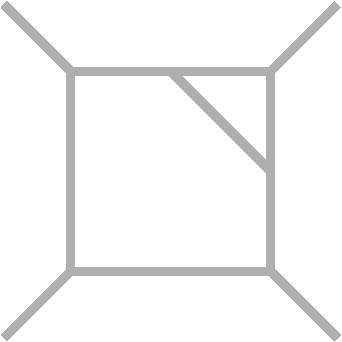
\includegraphics[width=\figureheight]{diagrams_from_4gluon/PentaTriangleThin}}};
        % Next-to-maximal
    \node at (0.5,1) (a) {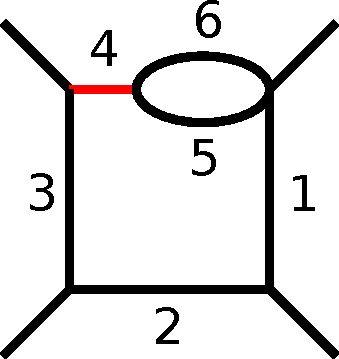
\includegraphics[width=\figureheight]{diagrams_from_4gluon/BubblePentagonSemiGenericThin}};
    \node at (0.5,0.5)  { $\Gamma_1^{\{1,1,1,1,1,1\}}$}; 
    \node at (1.5,1){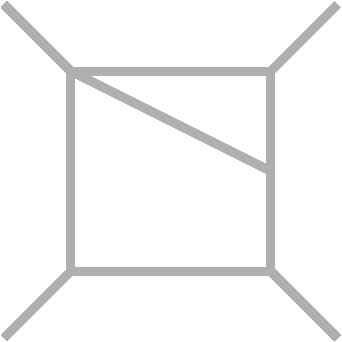
\includegraphics[width=\figureheight]{diagrams_from_4gluon/BoxTriangleThin}}; 
    \node at (2.5,1){\reflectbox{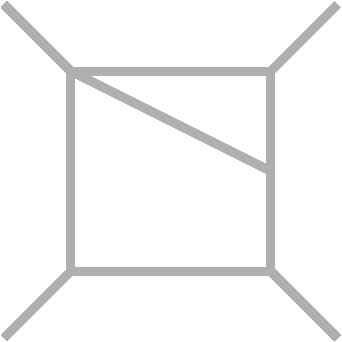
\includegraphics[width=\figureheight]{diagrams_from_4gluon/BoxTriangleThin}}};
        % Next-to-next-to-maximal
    \node at (1.5,0) (b) {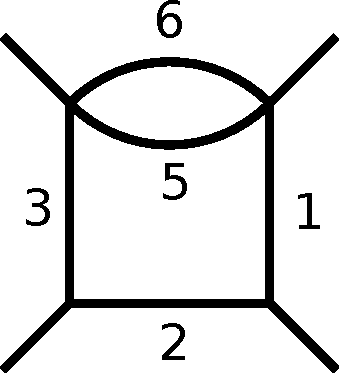
\includegraphics[width=\figureheight]{diagrams_from_4gluon/BubbleBoxGenericThin}};
    \node at (1.5,-0.5){$\Gamma_2^{\{1,1,1,1,1\}}$}; 
    \path [line,<->] (a.south east) -- (b.north west);
  \end{tikzpicture}
%
  \caption{A slice of the hierarchy of a two-loop four-point amplitude with the bubble-box topology $\Gamma_2$ at the bottom.
    The indices $i$ on the lines correspond to the propagators $\rho_i$, and the list of their exponents is given by the superscripts.
    One of the diagrams with topology $\Gamma_1$ has a doubled propagator $\rho_4$.
  }
  \label{fig:example_subleading_pole}
\end{figure}


}

\section{Evaluation of Cuts}
\label{sec:evaluation_of_cuts}

In this section we discuss evaluation of the left-hand side of the cut equations \eqref{eq:cut_equations}
in the factorized form of \cref{eq:cut_amplitude}.
For this we will need to know the explicit components of loop momenta solving the on-shell conditions for each topology.

\subsection{On-Shell Loop Momenta}
\label{sec:osm}

Given any topology $\Gamma$ with $N$ external momenta $\{p_1,\ldots{},p_N\}$, $L$ loops and $N_p$ propagators, our aim
is to find the components of $L$ loop momenta such that  
the cut conditions,
\[
  \rho_j = 0, \quad \forall j\in P_\Gamma,
\]
are satisfied. 
In principle the equations can be solved case by case given any initial choice of degrees of freedom.
However we would like the solution to be universal so that we can easily
implement it in a computer program once and for all. 
Furthermore, to be able to use it for both floating point and exact (finite field) numerical evaluations, 
we would like to avoid non-rational operations as much as possible.
The latter is in general non-trivial since the cut conditions are quadratic, and
define an algebraic variety in a $(D\cdot L)$-dimensional space.
To this end we closely follow the construction of ``natural'' coordinates described in \cite{Ita:2015tya, Abreu:2017xsl}.

\begin{figure}[ht]
  \centering
  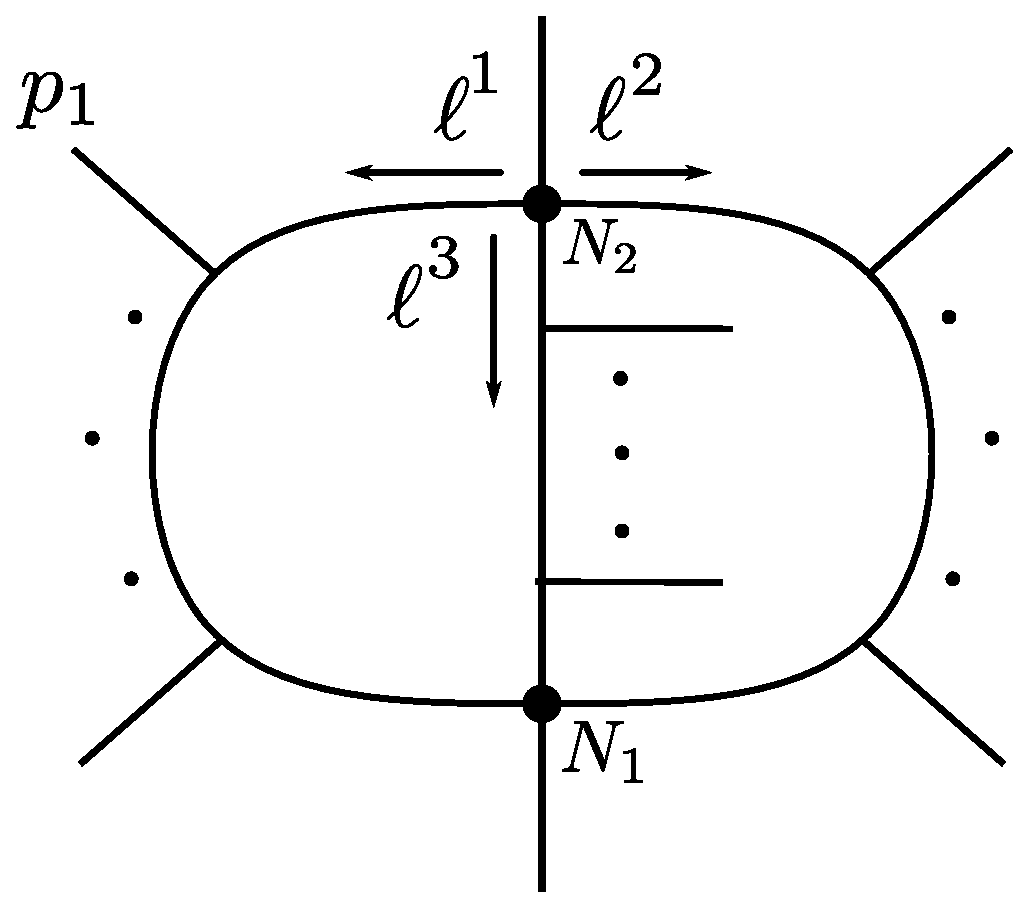
\includegraphics[width=0.3\textwidth]{topo_kinematics}
  \caption{A generic two-loop topology. All external momenta $p_i$ are outgoing. There are 3 strands connecting nodes $N_1$ and $N_2$.}
  \label{fig:topo_kinematics}
\end{figure}

We begin by considering each strand (see \cref{fig:topo_kinematics}) of the topology $\Gamma$ independently.
First we separate four-dimensional part and $(D-4)$-dimensional parts as
\begin{equation}
  \ell^l = \ell_{[4]}^l + \sum_{i\in \tilde{B}} \tilde{n}_j~\mu^l_{j}, \qquad \sp(\ell^l_{[4]},\tilde{n}) = 0, 
\end{equation}
where $\tilde{n}_i$ is some basis in $M_{[D-4]}$.
\todo{Unify the notion of spaces} 
For each strand $l$ we construct a van Neerven-Vermaseren basis (see \cref{sec:vNV_basis})
in $D=4$ with respect to the set $B^l = B^l_p \cup B^l_t$ of $\max(4,N-1)$ external momenta selected in the following order:
\begin{enumerate}
  \item momenta flowing out of strand $l$ (added to $B^l_p$),
  \item any other external momenta until $\max(4,N-1)$ of them is collected (added to $B^l_t$)
\end{enumerate}
Then for $\ell^l_{[4]}$ we get
\begin{subequations}
  \label{eq:lparametrization}
  \begin{align}
    \ell^l_{[4]} &= \sum_{j\in B^l_p} r^l_j(\vb*{\rho}^l)\,v^l_j ~+~ \sum_{j\in B^l_t} \alpha^l_j\,v^l_j ~+~\sum_{j\in B_\tau} \alpha^{\tau l}_j \frac{\tau_j}{(\tau_j)^2}, \\
    \label{eq:lparametrization_b}
    r_j^l(\vb*{\rho}^l) &=  \sp(\ell^l, p_j), \quad j\in B^l_p,    \\ 
    \label{eq:lparametrization_c}
    \alpha_j^l &=  \sp(\ell^l, p_j),\quad j\in B^l_t, \\
    \label{eq:lparametrization_d}
    \alpha_j^\tau &=  \sp(\ell^l, \tau_j),
  \end{align}
\end{subequations}
where $v^l_j$ are dual vectors to $p_j$, and $\tau_j$ are transverse to all external momenta of the topology.
We choose the propagators on the strand $l$, $\vb*{\rho}^l \in P_\Gamma^l \subset P_\Gamma$
as the first set of coordinates for our loop momenta. By construction $\cup_l P_\Gamma^l = P_\Gamma$,
so this trivially matches the choice of variables in \cref{chap:stdtech}.
The momentum conservation constraints from the nodes of the topology will
trivially match $\alpha_j^{\tau l}$ to the transverse ISPs from \cref{sec:ansatz_integrand},
and give \emph{linear} equations between $\alpha_j^l$ which can be used to
relate them to any choice of remaining ISPs $\hat{\vb*{\alpha}}$.
%This way we parametrized $4 L +\frac{1}{2}L(L+1)$ (recall \cref{eq:sps_all}) degrees of freedom from $(D\cdot L)$
%with the scalar products.
This in fact provides the lower bound on the dimension $D^{(L)}$ in which we can embed $L$ loop momenta
to be able to reproduce the required number of the scalar products,
\begin{equation}
  D^{(L)}  >  4 +\frac{1}{2}(L+1).
\end{equation}
The equality here cannot be taken except for the case of $L=1$ since we need additional degrees of freedom
(\todo{ask Harald how this can be explained properly from geometry})
for rotations.

What we achieved is that the on-shell conditions are trivialized,
and the only remaining constraints are for the components of $\va{\mu}_j$,
\begin{equation}
  \va{\mu}_i \cdot \va{\mu}_j  \equiv  \mu_{ij} (\vb*{\rho},\vb*{\alpha}) = \ell_i\cdot \ell_j - \ell_{i[4]}\cdot \ell_{j[4]},
\end{equation}
which can be easily solved once and for all.
Is is also possible to workaround the square roots appearing from this equations (see \cref{sec:muij_square_roots} for details),
so the parametrization can employed for computations with finite fields.

We conclude this section with two remarks.
\todo{
  In $D$ dimensions we don't have to worry about branches of solutions, 
  and also loop momenta can be real
}
Although in principle the parametrization described in this
section is amenable for both floating point and exact evaluations,
the former require the issues of numerical stability to be considered.
Ans in principle better suited parametrizations can be derived (see e.g.\ \cite{Kilgore:2007qr,Berger:2008sj} for one-loop examples),
which can be rather tedious already at one loop.

\subsection{Evaluation of Tree Amplitudes}

With the on-shell loop-momenta components available
we can evaluate the cuts in \cref{eq:cut_amplitude} as products
of tree amplitudes.

In \cref{eq:unitarity_ansatz} we have constructed  the basis of numerator insertions using Lorentz-invariants, and
the only explicit trace of the dimensional regularization was the presence of rational functions in $D$.
The evaluation of cuts in $D$ dimensions is much more involved since we need to treat the particles' states accordingly.
And a numerical evaluation is only possible if a finite (and preferably) small representation for these states exists.
In \cref{sec:osm} we found that thanks to Lorentz symmetry we can embed loop
momenta into a space with finite integer dimension $D^{(L)}$.
Taking advantage of this fact, we can embed the states of particles in a space of finite integer dimension $D_s\geq D^{(L)}$ as well.
From now on we will keep $D_s$ and $D$ separate,
and only after all master coefficients are determined will we set $D_s\to D\to 4-2\epsilon$.
In \cref{chap:dshel} we examine closely how to deal with the $D_s$-dependence efficiently.
In any case we need to be able to evaluate the tree amplitudes in arbitrary $D_s$ dimensions.

To this end we choose to utilize the off-shell Berends-Giele recursion \cite{Berends:1987me}
as a very flexible and efficient way to organize tree-level calculations
which admits a seamless generalization to $D_s$ dimensions.
The Berends-Giele recursion is formulated in terms of
\emph{off-shell currents} $J^{\bar{\alpha}}(\{p_i,\alpha^i\})$,
\begin{equation}
  \mathfigure{width=0.2\linewidth}{off-shell_current},
\end{equation}
defined as the sum of all possible ways (using the Feynman rules of the model)
to combine the legs with indices $\{\alpha^1,\ldots{},\alpha^n\}$ and
momenta $\{p_1,\ldots{},p_n\}$ into an open index of type $\bar{\alpha}$.
Here the indices $\alpha$ are understood to refer to tensor or spinor indices, as well as all other relevant quantum numbers such as
charge, flavor, color, etc.
Then starting from the first-level currents, which are simply the external states of particles, one
can recursively (see \cref{fig:BG_recution}) build up the final current
\begin{figure}[!ht]
  \centering
  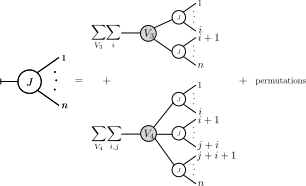
\includegraphics[width=0.8\textwidth]{BG_recursion}
  \caption{A step of the off-shell recursion for a model with 3- and 4-point vertices. All possible permutations of $\{1,\ldots{},n\}$ are considered on the right.}
  \label{fig:BG_recution}
\end{figure}
containing all but one external particles.
The tree amplitude is then obtained by contracting this current with the last remaining external state.
This topic is very well covered in the literature (see e.g.\ \cite{Ellis:2011cr,Weinzierl:2016bus}), so we will refrain from further details.

One of the consequence of unitarity is that the numerators of on-shell propagators are
sums over physical polarization states (in $D_s$ dimensions),
e.g.\ for spin 1 and spin $\frac{1}{2}$ particles
\begin{subequations}
  \begin{align}
    -g^{\mu\nu} + \frac{\ell^\mu \eta^\nu + \ell^\nu \eta^\mu}{\sp(\ell,\eta)}  &~\xleftrightarrow{\ell^2\to 0\;}~  \sum_{j=1}^{D_s-2} \varepsilon^\mu_j(\ell){\varepsilon^\nu_j}^{\star{}}(\ell) , \\
    \qty(\slashed{\ell}  \pm m\,\mathbb{1})^{\alpha\beta} &~\xleftrightarrow{\ell^2\to m^2}~ \sum_{j=1}^{2^{\frac{D_s}{2}-1}} u^\alpha_j(\ell){\overline{u}_j^\beta}(\ell),
  \end{align}
\end{subequations}
so on the cut we are allowed to switch back and forth.
The off-shell recursion provides a very convenient way to take advantage of this fact \cite{Badger:2012pg,Peraro:2016wsq}.
Consider \cref{fig:topo_cut}. Given a choice of a path along the cut,
we decompose into the state sums only the cut propagators at the beginning and at the end of the path.
Moving along the path, 
for each tree amplitude we build it's final current,
but instead of contracting it with the external state, we feed it through
the corresponding cut propagator as an input to the next tree amplitude.
Only at the end of the path do we contract the final current with a state from a polarization sum.
Note that beyond two loops it is not always possible to span the whole cut with just one continuous path.

\begin{figure}[ht]
  \centering
  \subfloat[\label{fig:topo_cut:path}]{
    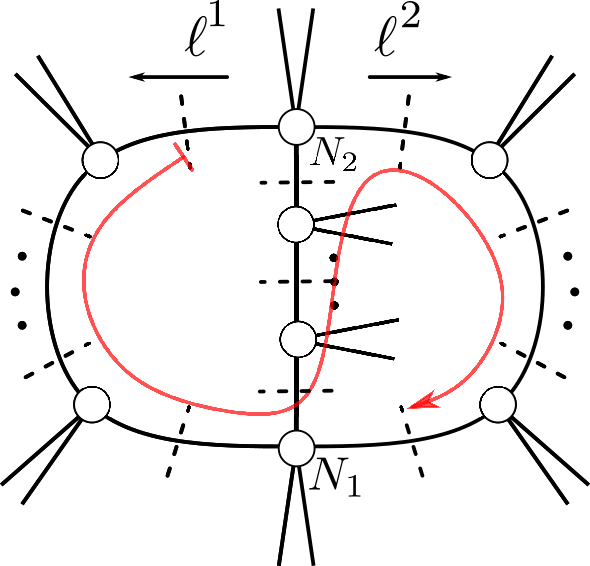
\includegraphics[width=0.3\textwidth]{topo_cut}
  }
  \hfill
  \subfloat[\label{fig:topo_cut:unrolled}]{
    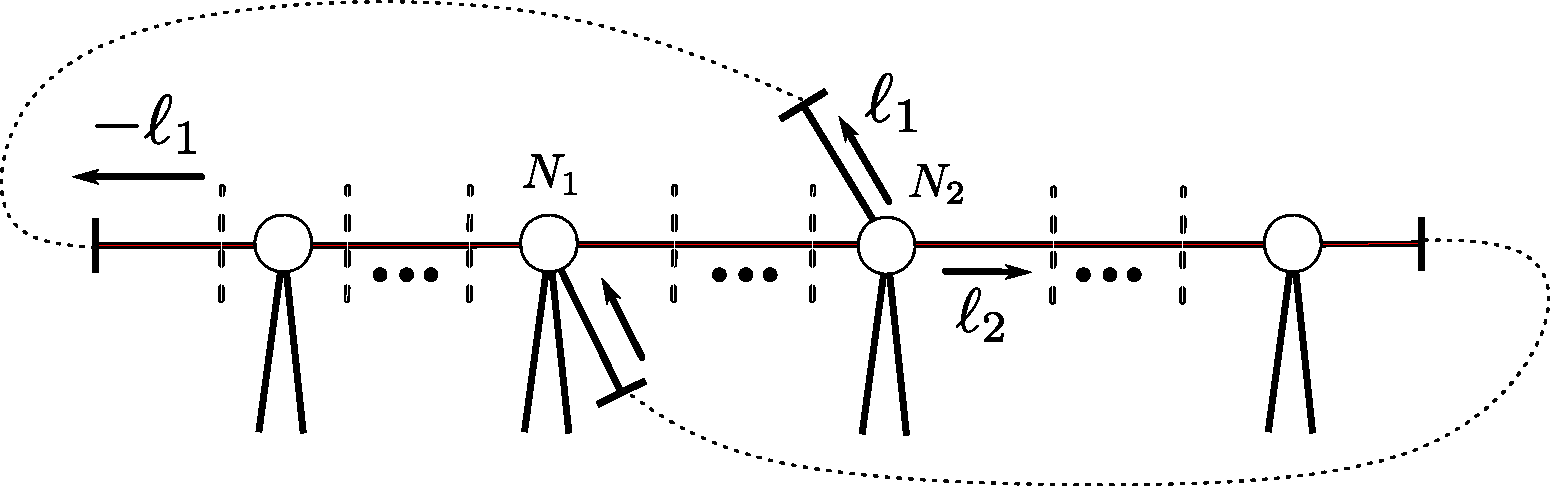
\includegraphics[width=0.6\textwidth]{topo_unrolled}
  }
  \caption{A generic cut of a two-loop amplitude as a sequence of ``closed'' off-shell currents, shown as blobs.
    The red line in \cref{fig:topo_cut:path} demonstrates a path, which is ``unrolled'' in \cref{fig:topo_cut:unrolled}.
    The dashed lines in \cref{fig:topo_cut:unrolled} indicate the only two cut propagators
    decomposed into pairs of polarization states and used as an explicit input to the off-shell recursion.
  }
  \label{fig:topo_cut}
\end{figure}

\todo{Gauge invariance is explicit in on-shell quantities, so no need to include ghosts.} 

\subsection{Dimensional Reconstruction}

We now have everything required to obtain the coefficients of master integrals 
$c_{\Gamma\gamma_\Gamma,i}$ from  \cref{eq:cut_equations}.  
\todo{equation solving?} 
The coefficients are functions of external kinematics $\vb*{x}$, and the dimensional regularization parameters $D$ and $D_s$.
In the spirit of our goal of constructing a fully numerically-capable framework, 
we can obtain the master coefficients
for any numerical value of $D$\footnote{
  here $D$ refers exactly to the parameter in the master/surface decomposition,
  and  not to be confused with the dimensionality of the space in which we embed loop momenta
}%
\textsuperscript{,}%
\footnote{as long as we avoid explicit poles on integer values},
and any  \emph{integer} value of $D_s$ large enough to embed the loop momenta components.
The internal self-consistency of dimensional regularization guarantees
that these evaluations reproduce correctly the corresponding limits from the formally infinite-dimensional spaces.\footnote{
  Beware of models with chiral couplings! A naive ``continuation'' of chirality to $D_s$ dimensions
  can make all coefficients to behave non-smoothly as functions of $D_s$ at all integer values.
}

We do however need to know the full analytic dependence on both $D$ and $D_s$ to be able
to set them to $4-2\epsilon$ eventually.
To this end we employ the function interpolation techniques (see \cref{sec:func_reconstruction})
and reconstruct the rational dependence on $D$ and polynomial dependence on $D_s$ for each coefficient from numerical samples.
This idea is known by the name of
\emph{dimensional reconstruction} \cite{Giele:2008ve,Ellis:2008ir,Boughezal:2011br,Abreu:2017xsl,Abreu:2017hqn}.
In some cases evaluating the left hand side of \cref{eq:cut_equations} for multiple $D_s$ values might become a computational bottleneck,
for example when fermionic particles appear in loops. In \cref{chap:dshel} we discuss how to address this issue.

We conclude this section with some technical remarks which
have important implications for numerical efficiency of the dimensional reconstruction.
\begin{itemize}
  \item Since the master integral coefficients depend both on $D$ and  $D_s$ at a first glance we would
    need to evaluate everything $n_D \cdot n_{D_s}$ times, where $n_D$ and $n_{D_s}$ are the sizes of the respective samples.
    However since the $D$-dependence comes solely from the right hand side of \cref{eq:unitarity_ansatz}
   and the $D_s$-dependence from the left hand side, we can sample each side independently only $n_D$ and $n_{D_s}$ times
   accordingly.
 \item Although we do need to determine the surface-term coefficients from \cref{eq:cut_equations} to use them for subtractions,
   we \textit{do not} need to reconstruct their dependence on $D$ analytically. 
   This is very helpful because the surface-term coefficients can be expected to be more complicated in general
   since they do not contain physical information and ambiguous to a great extent.
   %This is the first example of how numerical evaluations avoid the complexity of large intermediate expressions,
   %but the analytic result is obtained in still.
 \item The reconstruction algorithms normally work with exact numerical evaluations only.
   However even if we aim for example for Monte-Carlo integration over external phase space using floating point numbers,
   the rational functions of $D$ can be reconstructed for each process from just one exact ``warm-up'' evaluation over finite fields.
\end{itemize}

\section{Discussion}

In this chapter we laid out the central concepts of the multi-loop $D$-dimensional numerical unitarity approach.
We formulated it in a way directly amenable for automation.
And indeed we implemented the presented algorithms to obtain the results of \cref{chap:5parton}.

The major ingredients of our method, 
the master/surface integrand parametrization and
the usage of generalized cuts to obtain cut equations
are largely independent of each other and in fact 
can be used separately if deemed beneficial.

The cut equations can be employed to obtain the coefficients of any basis of integrand functions. 
For example, one can consider a basis of simple monomials in \cref{eq:rsp_reduction}.
In this way only the reduction of RSPs will be achieved, and the full IBP reduction has to be preformed afterwards.
One advantage is that the coefficients in this basis do not depend on $D$ (they still depend on $D_s$ of course).
Or one can consider the basis of simple monomials but with transverse ISPs traceless-completed (see \cref{sec:traceless_completion}).
In this way only the IBP reduction of non-transverse ISPs remains to be carried out \todo{reference this adaptive integrand reduction stuff?}.
The latter \textit{is} frequently the hardest part of the reduction of multi-loop amplitudes. 
So the fact that the master/surface basis mitigates significantly it's difficulty is the main argument for our choice.

It is also worth mentioning that the evaluation of cuts through the 
factorization property of \cref{eq:cut_amplitude} is not essential in our approach. 
The left hand side of \cref{eq:cut_equations} can in principle be any 
expression which has a form of \cref{eq:general_amplitude} which can be evaluated in the on-shell limit,
like a single Feynman diagram or a numerator insertion on a particular topology. 

%We usead cutting a lot.
%In our approach we made use of cutting in many places.
%``Unitarity'' approaches sometimes simply means anything employing cuts.

%Given the consideration above,

%On the opposite side the master/surface basis and do the full reduction in place.





%-------------------------------------------------

\chapter{Dimensional Regularization and Helicity Amplitudes
%in a Numerical Framework
}
\label{chap:dshel}
\newcommand\helampl{\mathcal{A}_{\vb*{\lambda}}}

In \cref{chap:stdtech,chap:numunitarity} we were operating on the objects under the assumption that they are Lorentz scalars.
However in QFT scattering amplitudes of particles with spin are not Lorentz scalars,
and the set of all Lorentz structures generated from Feynman diagrams is immensely redundant.
In this chapter we will discuss how amplitudes of any scattering process, 
polarized or not, can be decomposed into a minimal basis of Lorentz-invariant objects.

It is well known that the full physical information about any scattering process is contained in a complete set of \textit{helicity amplitudes} ---
the amplitudes with all external particles' states chosen to have a definite helicity (see the definition in \cref{chap:4dspinhel}).
Being non-redundant and a complete representation of physical information, the helicity amplitudes 
enjoy a number of nice properties such as gauge invariance and manifestation of Poincaré symmetry.
On a technical side, the consequence is that the helicity amplitudes are expected to have the most compact representation,
given that they do not suffer from proliferation of unphysical information.
And indeed this has been shown to be the case in numerous practical applications (see e.g.\ %
\cite{DeLaurentis:2019phz,Badger:2019djh,Badger:2011yu,Badger:2013gxa,DeFreitas:2004kmi,Gehrmann:2011aa,Gehrmann:2009vu,Glover:2004si,Glover:2003cm,Garland:2002ak,Dunbar:2016aux,Dunbar:2016gjb,Dunbar:2016cxp,Badger:2015lda,Gehrmann:2015bfy,Bern:2003ck,Bern:2002tk,Badger:2018enw,Dunbar2017,Kunszt:1994nq}).

The computation of tree-level helicity amplitudes is a very straight-forward task,
which, from the perspective of Feynman diagrams,
amounts to simply inserting the corresponding states with definite helicities for each external particle.
Spinor-helicity techniques can be employed to further enhance the computations.
Moving forward to amplitudes with loops,
we are forced to make the dimensionality of space-time formally infinite \cite{Collins:1984xc} 
to regularize divergences.%
\footnote{
  A possibility to formulate the dimensional regularization in finite vector spaces was explored in \cite{Weinzierl:1999xb}.
  We do not pursue it here.
}%
\textsuperscript{,}%
\footnote{
  Other regularization methods are out of the scope of this thesis.
}
This fact makes both definition and evaluation of helicity amplitudes rather delicate.
It is the purpose of this chapter to present a concise and efficient method of
evaluating multi-loop helicity amplitudes in dimensional regularization,
amenable for numerical applications.

In \cref{sec:helampl_projectors} we briefly review a somewhat standard 
method of obtaining helicity amplitudes through $D$-dimensional projectors,
which can be found in the literature\footnote{
  See also related work in \cite{Chen:2019wyb,Boels:2018nrr}. 
} \cite{Garland:2002ak, Moch:2002hm, Glover:2003cm, Glover:2004si,Gehrmann:2009vu,Gehrmann:2011aa}.
In \cref{sec:helampl_embeding}, 
taking advantage of some insights from \cref{chap:numunitarity},
we show how the tree-level approach of ``simply inserting appropriate external states'' can
be extended to loop amplitudes in the 't Hooft-Veltman (HV) flavor of dimensional regularization.
This allows to dispose of the construction of complicated projectors, which
becomes very hard to handle for large $(> 4)$ number of particles with spin \cite{Peraro:2019cjj}. 
Another convenient feature of our approach is that it can be applied in a numerical context, such
as evaluation of cuts through off-shell recursion as discussed in \cref{sec:evaluation_of_cuts}.
In \cref{sec:ds_reduction} we discuss how
the efficiency of extraction of the full $D_s$ dependence can be substantially improved
by dimensionally reducing kinematically-independent degrees of freedom in higher dimensions.

The content of this chapter is based on the parts of \cite{Anger:2018ove,Abreu:2018jgq,Abreu:2019odu}.

\section{Helicity Amplitudes}
\label{sec:HV_helicity_amplitudes}

A helicity amplitude $\helampl$
is defined as an $\mathcal{S}$-matrix element
with external polarization states $\varepsilon_{i}$ chosen to be
helicity eigenstates (for the definition of helicity see \cref{chap:4dspinhel}) with helicities $\vb*{\lambda}=\{\lambda_1,\ldots{},\lambda_N\}$.
Cross sections obtained from $\Abs{\helampl{}}$ describe
the scattering of polarized particles.
Unpolarized cross sections can be obtained by summing over the helicities of all external particles.
Helicity states satisfy the completeness relations
\begin{subequations}
  \label{eq:4d_completeness_relations}
  \begin{align}
    \sum_{\lambda=\{+1,-1\}} \varepsilon^\mu_\lambda(p){\varepsilon^\nu_\lambda}^{\star{}}(p)  &= -g^{\mu\nu} + \frac{p^\mu \eta^\nu + p^\nu \eta^\mu}{\sp(p,\eta)}, \\
    \sum_{\lambda=\{+\frac{1}{2},-\frac{1}{2}\}} u^\alpha_\lambda(p){\overline{u}_\lambda^\beta}(p)  &= \qty(\slashed{p}  \pm m\,\mathbb{1})^{\alpha\beta},
  \end{align}
\end{subequations}
for gauge bosons and fermions correspondingly.
The number of $N$-particle helicity amplitudes is thus $2^N$, but
the number of of independent analytic expressions can be further reduced by taking into account charge and parity transformations.

The transformation of helicity amplitudes under Lorentz boosts is completely specified by their 
external states, and is given by the \emph{little group scaling},
\begin{equation}
  \ket{p_i} \to t_i \ket{p_i}, \quad  \sket{p_i} \to \frac{1}{t_i} \sket{p_i} \implies \helampl \to  \qty(\prod_i t_i^{-2\lambda_i}) \helampl,
\end{equation}
where $t_i$ are complex phases.
As expected the squared matrix element $\Abs{\helampl{}}$ is Lorentz-invariant.
With the help of the spinor helicity formalism we can also make any helicity amplitude itself into a scalar
by removing it's \emph{spinor weight} --- a factor which has the same little group scaling
as the helicity amplitude.
Hence the scalar objects we were operating on in \cref{chap:stdtech,chap:dshel} can be the normalized helicity amplitudes.

We can perturbatively expand helicity amplitudes in the coupling constants as
\begin{equation}
  \helampl =  \helampl^{(0)} + g^2 \helampl^{(1)} + g^4 \helampl^{(2)} + \ldots{},
\end{equation}
with all leading-order couplings absorbed into $\helampl^{(0)}$.
It is then convenient to use the tree helicity amplitude\footnote{if it is not vanishing} $\helampl ^{(0)}$ to remove the spinor weight
of loop amplitudes.
It should be noted that the definition of polarized cross sections may not depend on a regularization scheme
used to regularize divergences of loop amplitudes. This implies, that 
among the flavors of dimensional regularization only in the ones which consider external particles 
to be in four dimensions the helicity amplitudes can be consistently defined.

%This can be achieved for example by normalizing all amplitudes $A^{L}_N$ with $L\geq1$ by
%a corresponding tree amplitude $A^{0}_N$ 

\section{Form Factor Decomposition and Projectors}
\label{sec:helampl_projectors}

In this section we review the conceptually simplest way to define helicity amplitudes in dimensional regularization, which is through $D$-dimensional projectors.
This approach has been used in a number of computations (see e.g.\ \cite{Garland:2002ak, Moch:2002hm, Glover:2003cm, Glover:2004si,Gehrmann:2009vu,Gehrmann:2011aa}).
Its relation to HV scheme and helicity amplitudes has been recently discussed in \cite{Peraro:2019cjj}.

One starts with decomposing an amplitude with \emph{unspecified} external states into all possible $D$-dimensional tensor structures $\mathcal{T}_i$ compatible
with symmetries and gauge invariance,
\begin{equation}
  \mathcal{A}  = \sum_{i} \mathcal{T}_i\;A_i.
\end{equation}
For example $\mathcal{T}_i$ can contain objects like $\sp(\varepsilon(p_i),p_j)$, $\bar{v}(p_i) \slashed{p}_j u(p_k) $, $\bar{u}(p_i) \slashed{\varepsilon}(p_j) u(p_k)$, etc.
Here $A_i$ are the Lorentz-invariant form factors.
Then one finds projectors $\mathcal{P}_i$ on $A_i$ from linear combinations of $\mathcal{T}_i$ by solving the equations
\begin{equation} \label{eq:cdr_projectors}
  \mathcal{P}_i [\mathcal{A}] = \qty(\sum_j c_{i,j}(\vb*{x},D) \sum_\text{(states)} \mathcal{T}^{\dagger}_j) \qty[\sum_{k} \mathcal{T}_k A_k] = A_i, 
\end{equation}
for the coefficients $c_{i,j}(\vb*{x},D)$, which are rational functions of external kinematics $\vb*{x}$ and $D$.
Here the state sums are taken to be in $D$ dimensions, which corresponds to working in the CDR scheme.

To extract the helicity amplitudes one then \textit{evaluates} the tensor structures $\mathcal{T}_i$ 
by inserting the corresponding \textit{helicity states in four dimensions} for each of the external particles. 
This is equivalent to switching to the HV scheme.
The procedure uncovers the fact that only particular linear combinations of $A_i$ are relevant,
and the number of these combinations is exactly the number of independent helicity amplitudes, which is
significantly lower than the number of initial tensor structures $\mathcal{T}_i$.

The difficulties of this approach are two-fold:
\begin{enumerate}
  \item The number of initial tensor structures grows very fast with the number of external particles with spin.
    This makes solving the equations \cref{eq:cdr_projectors} for projectors and then applying them to each Feynman diagram very challenging for $N>4$.
  \item The projectors have to be applied to analytic expressions since the external states in $D$ dimensions do not admit any finite numerical representations \cite{Collins:1984xc}.
\end{enumerate}

Since the helicity amplitudes contain the complete physical information, 
the construction of form factors in  \cref{eq:cdr_projectors} seems to be an unnecessary complication.
And indeed a way to avoid these steps and construct the projector onto helicity amplitudes directly has been suggested recently \cite{Peraro:2019cjj}.
This somewhat mitigates the first issue, but the projectors have to be still applied to analytic expressions.

\section{Helicity Amplitudes from Embedding of External States}
\label{sec:helampl_embeding}

In this section we explain how multi-loop helicity amplitudes
with vector and spinor external particles can be obtained in dimensional regularization
from appropriate embedding of helicity states into spaces of higher dimensionality $\mathsf{S}_{[D_s]}$.
As in \cref{sec:evaluation_of_cuts}, in this \namecref{chap:dshel} we will denote the dimensionality of the particles'
representations as $D_s$.
Our approach is built up independently from the one described in the previous chapter, but we establish
the connection in the end.

In HV the space-time symmetry group is extended to $\mathrm{SO}(1,D_s-1)$, and the external particles are kept in four dimensions. 
More precisely this means that, like in CDR, the tensor and Clifford algebras are performed in $D_s$ dimensions,
but the completeness relations for external states have to be as in \cref{eq:4d_completeness_relations}. 
In other words the amplitudes in HV transform like their four-dimensional counterpart under $\mathrm{SO}(1,3)$, 
and are invariant under the rotations in $\mathrm{SO}(D_s-4)$. 
This implies that, upon normalizing by an appropriate spinor weight, the helicity amplitudes are scalars of the extended symmetry group $\mathrm{SO}(1,D_s-1)$.
In \cref{chap:numunitarity} we argued that we can use this symmetry to embed the formally infinite-dimensional computation
into a finite one with appropriately chosen integer values of $D^{(L)}$ and $D_s$.
This fact motivates our strategy:
\begin{enumerate}
  \item Consider amplitudes in arbitrary (integer) $D_s \geq  D^{(L)}$ dimensions with fixed external states,
    which have the right little-group behavior with respect to $\mathrm{SO}(1,3) \subset \mathrm{SO}(1,D_s-1)$.
  \item Impose the rotational symmetry in $\mathrm{SO}(D_s-4)$ by combining the degrees of freedom from $\mathsf{S}_{[D_s-4]}$ in
    a suitable way.
  \item Set $D_s\to D$ in the amplitudes obtained from the previous step (which are polynomials in $D_s$).
\end{enumerate}
As we will see shortly, the second step is trivial for vector particles. For fermionic
particles it requires a tensor decomposition similar to the one we discussed in \cref{sec:helampl_projectors},
but enormously simplified by the fact that the indices in  $\mathsf{S}_{[D_s-4]}$ are completely decoupled from kinematics\footnote{
  this applies after the loop integrations are performed, 
  but we can always pull the corresponding projectors into the integrand given that $D_s$ was not set to $D$ yet.
}
and that we can ignore all vector particles.



\subsection{Embedding of Vector States}
\label{sec:embedding_vectors}
Consider the amplitudes for the scattering of massless vector particles.
There are $(D_s - 2)$ states for each particle in $D_s$ dimensions. 
The corresponding polarization sum for a particle with momentum $p$ is 
\begin{equation} \label{eq:vector_pol_sum_ds}
  \sum_{j=1}^{D_s-2} \varepsilon^\mu_j(p){\varepsilon^\nu_j}^{\star{}}(p) = -g_{[4]}^{\mu\nu} + \frac{p^\mu \eta^\nu + p^\nu \eta^\mu}{\sp(p,\eta)} \;-\; g_{[D_s-4]}^{\mu\nu}, 
\end{equation}
where we used $p \in \mathsf{S}_{[4]}$
to make the $(D_s-4)$-dimensional part explicit.
Comparing this to \cref{eq:4d_completeness_relations} we see that we can embed the helicity states as \cite{Kosower:1990ax}
\begin{align} \label{eq:embedding_vectors}
  \varepsilon_{1,2}^\mu =
    \begin{dcases}
      \varepsilon^\mu_{+,-}, & \mu\in \mathsf{S}_{[4]},\\
      0, & \mu\in \mathsf{S}_{[D_s-4]},\\
    \end{dcases}
    &&
  \varepsilon_{j}^\mu = \delta^\mu_{(j+1)}, \qfor j\geq 3,
\end{align}
Thus, the amplitudes in $D_s$ dimensions with $\varepsilon_{1,2}^\mu$ as external states satisfy the correct little-group scaling trivially.
If we now also take into account the orthogonality relations 
\begin{align}
  g_{[D_s]}^{\mu\nu} = g^{\mu\nu}_{[4]}+g^{\mu\nu}_{[D_s-4]}, && (g_{[4]})^{\mu\rho}(g_{[D_s-4]})_{\rho\nu} = 0,
      %& (g_{[x]})^{\mu}_\mu =x, \qfor x \in  \{4,D_s,D_s-4\},
\end{align}
we see that these amplitudes are invariants under the rotations in $\mathsf{S}_{[D_s-4]}$.
Hence they are the helicity amplitudes in the HV scheme.
This is, of course, a well-known fact which has been exploited in one-loop computations with numerical generalized
unitary methods \cite{Ellis:2007br,Giele:2008ve}, as well as as 
in the so-called six-dimensional helicity formalism \cite{Bern2011,Cheung:2009dc,Badger:2013gxa,Badger:2017jhb}.

Note that, in contrast to the form factor decomposition in \cref{sec:helampl_projectors}, we did not need any projectors.

\subsection{Embedding of Spinor States}
\label{sec:embedding_spinors}

We now consider amplitudes with external fermions.
There are $2^{\frac{D_s}{2}-1}$ spinor states in $D_s$ dimensions, 
which can be constructed through the representations of Clifford algebras (see \cref{sec:clifford_algebra_ds}).
The polarization sum with the momentum $p \in \mathsf{S}_{[4]}$ is
\begin{equation} \label{eq:ds_spin_polsum}
  \sum_{j=1}^{2^{\frac{D_s}{2}-1}} u^\alpha_j(p){\overline{u}_j^\beta}(p) = \qty(\slashed{p}_{[D_s]}  \pm m\,\mathbb{1}_{[D_s]})^{\alpha\beta} \equiv 
  \qty(\slashed{p}_{[4]} \pm m \cdot \mathbb{1}_{[4]})^{\bar{\alpha}\bar{\beta}} \qty(\mathbb{1}_{[D_s-4]})^{\hat{a}\hat{b}},
\end{equation}
where the indices $\alpha = \bar{\alpha}\otimes\hat{\alpha}$,  $\beta = \bar{\beta}\otimes \hat{\beta}$ are factorized into 
$\{\bar{\alpha},\bar{\beta}\}\in \mathsf{S}_{[4]}$ and $\{\hat{\alpha},\hat{\beta}\}\in \mathsf{S}_{[D_s-4]}$.
Comparing to \cref{eq:4d_completeness_relations}, we see that we can embed the four-dimensional spinors as
\begin{align} \label{eq:fermionicStates}
    \qty(u_{\lambda,i})^{\bar{\alpha}\hat{\alpha}} =  u_{\lambda}^{\bar{\alpha}} \cdot \delta_i^{\hat{\alpha}}, && i = 1,\ldots{},2^{\frac{D_s}{2}-2},
\end{align}
where we replaced the index $j$ in \cref{eq:ds_spin_polsum} by $\{\lambda, i \}$ to make the four-dimensional helicity $\lambda \in  \{+\frac{1}{2},-\frac{1}{2}\}$ manifest.
Thus the amplitudes in $D_s$ dimensions with any of the spinors $\qty(u_{\lambda,i})^{\bar{\alpha}\hat{\alpha}}$ taken as external fermionic states\footnote{
  The fact the these spinors also satisfy the Dirac equation in $D_s$ dimension can be easily verified.
}
(and with the vector states taken as in \cref{sec:embedding_vectors}) have the correct little-group scaling.
However, as opposed to the case of vector particles, we observe that 
all of the states in \cref{eq:fermionicStates} introduce a \emph{preferred direction} in  $\mathsf{S}_{[D_s-4]}$
via the indices $\hat{\alpha}$.
Hence the amplitudes with a particular choice of $\qty(u_{\lambda,i})^{\bar{\alpha}\hat{\alpha}}$ are \textbf{not} symmetric under the rotations $\mathrm{SO}(D_s-4)$.
From a different point of view, we have many states with the same helicity, which creates an ambiguity as to what 
should be the helicity amplitude.
On that account, we turn to the tensor decomposition of indices $\hat{\alpha}$.

\subsection{Tensor Decomposition in \texorpdfstring{$D_s-4$}{Ds-4}}
\label{sec:HelAmplHV}

We decompose an amplitude with external fermions in $D_s$ dimensions as
\begin{equation} \label{eq:tensorDecomposition}
  \mathcal{A} = \sum_n v_n A_n,
\end{equation}
where all spinor indices $\hat{\alpha}_i \in \mathsf{S}_{[D_s-4]}$ (and only them) are absorbed into $v_n$,
and, consequently, $A_n$ are scalars of $\mathsf{S}_{[D_s-4]}$.
In the following we will show how to construct a convenient basis of the tensor structures $v_n$ 
for any number of external fermions.

First we observe that only the spinor chains of the form
\begin{equation} \label{eq:generic_dsm_4_schain}
  u^{\hat{\alpha}}_i \; \qty( \prod_k \gamma^{\mu_k}_{[D_s -4 ]} )^{\hat{\alpha}\hat{\beta}} \; u^{\hat{\beta}}_j \quad\equiv\quad 
  \qty( \prod_k \gamma^{\mu_k}_{[D_s -4 ]} )^{i j},
\end{equation}
with indices $\mu_i \in \mathsf{S}_{[D_s -4]}$ contracted to other spinor chains, contribute to $v_n$.
This is the consequence of the following facts:
\begin{itemize}
  \item Thanks to our choice of states for vector particles, all Lorentz vectors, which can be contracted with $\gamma^{\mu_i}_{[D_s]}$,
    project them into $\mathsf{S}_{[4]}$:
    \begin{align} \label{eq:trivialTens1}
      a_{\mu}
      \left( \gamma_{[D_s]}^\mu \right)_{\bar{\alpha}\hat{\alpha}}^{\bar{\beta}\hat{\beta}} =
      a_{\mu}\left(\gamma_{[4]}^\mu \right)_{\bar{\alpha}}^{\bar{\beta}} \delta_{\hat{\alpha}}^{\hat{\beta}}\,,
      &&
      a \in \{p_i,\varepsilon_{1,2}(p_i)\}
    \end{align}
    This has an effect that no kinematic-dependence can enter $v_n$.
  \item Any Lorentz indices inside the same spinor chain can be contracted yielding  
    \begin{equation} \label{eq:trivialTens2}
      \left(\gamma_{[D_s]}^\mu\right)_{\bar{\alpha}\hat{\alpha}}^{\bar{\kappa}\hat{\kappa}}
      \left(\gamma_{[D_s]\mu}^{\phantom{\mu}}\right)_{\bar{\kappa}\hat{\kappa}}^{\bar{\beta}\hat{\beta}}
      =D_s~\delta_{\bar{\alpha}}^{\bar{\beta}}\delta_{\hat{\alpha}}^{\hat{\beta}}\,.
    \end{equation} 
  \item Due to the factorized representation of the Clifford algebra (see \cref{eqn:cliffordrecursion}), any spinor chain can be written in a factorized form.
\end{itemize}
Non-trivial tensors $v_n$ are thus obtained by contracting
Lorentz indices between multiple chains of  matrices $\gamma_{[D_s-4]}$.
Some examples of possible $v_n$ are
\begin{equation}
  \begin{aligned}
    & \delta^{i_1}_{j_1} \delta^{i_2}_{j_2},\\
    & (\gamma_{[D_s-4]}^{\mu_1} )_{i_1}^{j_1} (\gamma_{[D_s-4]\mu_1}^{\phantom{\mu}})_{i_2}^{j_2}, \\
    & (\gamma_{\mu_1[D_s-4]}^{\phantom{\mu}} )_{i_1}^{j_1} (\gamma_{[D_s-4]}^{\mu_1}\gamma_{[D_s-4]}^{\mu_2} )_{i_2}^{j_2} (\gamma_{[D_s-4]\mu_2}^{\phantom{\mu}})_{i_3}^{j_3},\\
    & \qquad \vdots{}
  \end{aligned}
\end{equation}

To construct a basis of tensor structures $v_n$ we can decompose each of the spinor chains entering it
into the standard basis of anti-symmetrized products of gamma-matrices (see e.g.\ \cite{Veltman:1988au}),
\begin{align}\label{eq:basisGammaChainDs}
\gamma_{[D_s-4]}^{\mu_1 \ldots \mu_n} = \frac{1}{n!} \sum_{ \sigma\in S_n} \sgn(\sigma) \gamma_{[D_s-4]}^{\mu_{\sigma(1)}} \ldots \gamma_{[D_s-4]}^{\mu_{\sigma(n)}}\,,
\end{align}
where $S_n$ is the set of all permutations of $n$ integers, and $\sgn(\sigma)$ is the signature of the permutation $\sigma\in S_n$.
It can be shown (see \cref{sec:identities}), that the
projectors $\mathcal{P}_n$ onto $v_n$ can be constructed from the conjugated tensors $v_n^\dagger$ as
\begin{align} \label{eq:dsm_4_projectors}
  \mathcal{P}_n [v_m] \coloneqq \qty(\prod_{s=1}^{n_s} \Tr_s) v_n^\dagger\; v_m = c_n(D_s-4)~\delta_{n m},  %&& c_n = \frac{(D_s-4)!\,n!}{(D_s-4-n)!},
\end{align}
with the traces are taken over each of $n_s$ spinor chains, and we drop the irrelevant total factor of $\qty(\Tr\mathbb{1}_{[D_s -4 ]})^{n_s}$.
The coefficients $c_n$ can be computed for each $n_s$ combinatorially, as demonstrated in \cref{eq:cnCalc}.
We emphasize that, unlike the projectors in \cref{sec:helampl_projectors}, the ones in \cref{eq:dsm_4_projectors}
operate on the explicitly-represented objects, hence can be evaluated numerically.
We now consider two examples.

\paragraph{One pair of external fermions.}
As a first and trivial example we consider an amplitude with one pair of external fermions (and any number of external gauge bosons). 
There is only a single chain of matrices $\gamma_{[D_s-4]}$, so
there is only a single term in the decomposition of \cref{eq:tensorDecomposition},
\begin{equation}\label{eq:decompqqbar}
  \mathcal{A} =v_0\,A_0\,,\qquad \textrm{with}\quad (v_0)_{\hat{\alpha}}^{\hat{\beta}}=\delta_{\hat{\alpha}}^{\hat{\beta}}\,.
\end{equation}
\paragraph{Two pairs of distinct fermions.}
As a second example we consider an amplitude with two fermion pairs of different flavors, (and any number of gauge bosons). 
The basis $\{v_n\}$ consists of contractions between two spinor chains of the form \cref{eq:generic_dsm_4_schain}:
\begin{align}
  \begin{split} \label{eqn:4qtensors}
    (v_0)_{j_1j_2}^{i_1i_2}   = &
    \delta_{j_1}^{i_1} \delta_{j_2}^{i_2}\,, \\
    (v_1)_{j_1j_2}^{i_1i_2}=
    &(\gamma_{[D_s-4]}^{\mu_1} )_{j_1}^{i_1} 
    (\gamma_{[D_s-4]\mu_1}^{\phantom{\mu}})_{j_2}^{i_2}\,, \\
    & \vdots\\
    (v_k)_{j_1j_2}^{i_1i_2}=
    &(\gamma_{[D_s-4]}^{\mu_1 \ldots  \mu_k})_{j_1}^{i_1}
    (\gamma_{[D_s-4]\mu_1 \ldots \mu_k}^{\phantom{\mu}})_{j_2}^{i_2}\,,\\
    & \vdots\,
  \end{split}
\end{align}
The number of elements in the basis $\{v_n\}$ depends on $D_s$,
and is infinite for non-integer $D_s$ (because the basis of the Clifford algebra \cref{eq:basisGammaChainDs} is infinite).
But for any given number of loops $L$ only a finite number of basis elements $n^{(L)}\coloneqq \dim\{v_n\}$ can appear.
This number can be found from inspecting the diagrams without external gauge bosons 
with maximal number of propagators.
For instance we have $n^{(0)}=0$, $n^{(1)}=3$ and $n^{(2)}=5$.

Each coefficient $A_n$ in the decomposition of \cref{eq:tensorDecomposition} satisfies our desiderata 
of the HV amplitudes from \cref{sec:HV_helicity_amplitudes}, so, in principle, we need to determine all of them to obtain the full amplitude.
In the next section we argue that, at least to NNLO, it is not the case, 
and all physically-relevant information can be extracted from just one coefficient.  

\subsection{Relevant Coefficients}
\label{sec:relevant_tensors}

It was shown in \cite{Weinzierl:2011uz} that for NNLO computations only the $\order{\eps^0}$ terms of the 
\emph{finite remainders} $\mathcal{F}^{(1)}$ and $\mathcal{F}^{(2)}$ of one- and two-loop amplitudes are required.
They are defined by subtracting the universal divergent structure of one- and two-loop amplitudes, 
\begin{subequations}
  \begin{align}
    \label{eq:F0}
    \mathcal{F}^{(0)} &\coloneqq \mathcal{A}^{(0)}, \\ 
     \label{eq:F1}
    \mathcal{F}^{(1)} &\coloneqq \mathcal{A}^{(1)} - \mathbf{I}^{(1)} \mathcal{A}^{(0)}, \\ 
     \label{eq:F2}
    \mathcal{F}^{(2)} &\coloneqq \mathcal{A}^{(2)}  - \mathbf{I}^{(1)} \mathcal{A}^{(1)} - \mathbf{I}^{(2)} \mathcal{A}^{(0)}.
  \end{align}
\end{subequations}
The operators $\mathbf{I}^{(1)}$ and $\mathbf{I}^{(2)}$ can be found in \cite{Catani:1998bh,Sterman:2002qn,Becher:2009cu,Gardi:2009qi}.\footnote{
  We also include renormalization into these operators, which is possible in massless QCD.
  Alternatively we simply consider $\mathcal{A}^{(L)}$ to denote renormalized amplitudes in this section.
}
Here for convenience we also introduced a finite remainder for tree amplitudes, which is simply an alias for the amplitude itself.
We can expand both sides of \cref{eq:F0,eq:F1,eq:F2} in terms of tensor structures of \cref{eq:tensorDecomposition}
to get the corresponding coefficients $\mathcal{F}^{(i)}_n$ of the finite remainders.
The cross section is obtained by squaring the finite remainders, possibly multiplied by some
finite operator $\mathbf{F}$ (we refer to \cite{Weinzierl:2011uz} for details),
\begin{equation} \label{eq:Fsq}
  \Re\qty(\mathcal{F}^{\dagger(i)}\mathbf{F}\mathcal{F}^{(j)}) = \sum_m\sum_n\; \mathcal{P}_m \qty[v_n]  \; \Re\qty(\mathcal{F}^{\dagger(i)}_m\mathbf{F}\mathcal{F}^{(j)}_n) = 
     \sum_n c_n \; \Re\qty(\mathcal{F}^{\dagger(i)}_n\mathbf{F}\mathcal{F}^{(j)}_n),
\end{equation}
where in the last equality we used \cref{eq:dsm_4_projectors}.
For non-identical pairs of fermions\footnote{We discuss identical fermions below.} 
the first element of the basis $\{v_n\}$ is
\begin{equation}
  v_0  = \delta^{\hat{\alpha}_1}_{\hat{\beta}_1}\cdots \delta^{\hat{\alpha}_{n_s}}_{\hat{\beta}_{n_s}},
\end{equation}
and the corresponding coefficient $c_0 = 1$.
As demonstrated in \cref{sec:identities}, the coefficients of all other tensor structures
contribute to higher orders in $\eps$ when we set $D_s\to 4-2\eps$,
\begin{equation}
  c_i=\order{\eps}, \qfor i\geq 1,
\end{equation}
and we can drop all $\order{\eps}$ terms in \cref{eq:Fsq}.
Thus, we conclude that all we need to know is the coefficient of $v_0$.


\subsubsection{Identical Fermions}
To illustrate how to handle the cases with identical fermions,
we consider an amplitude with two pairs of fermions with the same flavor. 
It can be constructed by anti-symmetrizing the corresponding amplitude with distinct flavors.
In this way, we start from the basis in \cref{eqn:4qtensors},
and extend it with anti-symmetrized tensors $\{\tilde v_n\}$ as
\begin{equation}\label{eq:basisIdentical}
	(\tilde v_n)_{j_1j_2}^{i_1i_2} \coloneqq  (v_n)_{j_1j_2}^{i_2i_1}\,,
\end{equation}
so our basis is now $\{v_n\}\cup \{\tilde{v}_n\}$.
It satisfies the following properties:
\begin{equation}\label{eq:dualBasisIdentical}
  \mathcal{P}_n[v_m]= c_n \delta_{m n}\,,\qquad
  \mathcal{\tilde{P}}_n[\tilde{v}_m]= \tilde{c}_n \delta_{m n}\,,\qquad
  \mathcal{P}_n[\tilde{v}_m] = \delta_{m 0}\,\delta_{n 0}+\mathcal{O}(\epsilon)\,.
\end{equation}
The coefficients in the first two equations are the same as for the case of distinct fermions. 
We do not provide the closed form for the coefficients in the last equation, but
we verified the fact that they are proportional to $(D_s-4)$ for $m,n>0$.

Now consider the interference between the two-loop finite remainder and 
the corresponding tree amplitude, which should be anti-symmetrized over flavors individually,
\begin{multline}
  \qty(\mathcal{F}^{(0)} - \mathsf{f}\circ\mathcal{F}^{(0)})^\dagger \cdot 
    \qty(\mathcal{F}^{(2)} - \mathsf{f}\circ\mathcal{F}^{(2)}) = \\
    \qty(\mathcal{P}_0\qty[\mathcal{F}^{(0)}] - \mathcal{P}_0\qty[\mathsf{f}\circ\mathcal{F}^{(0)}])^\dagger \cdot 
    \qty( \mathcal{P}_0\qty[\mathcal{F}^{(2)}] - \mathcal{P}_0\qty[\mathsf{f}\circ\mathcal{F}^{(2)}]) ~+~ \order{\epsilon}.
\end{multline}
Here the application of $f\circ$ exchanges the flavors. 
On the right hand side we used the identities from \cref{eq:dualBasisIdentical} to
show that, to $\order{\epsilon}$, 
we can anti-symmetrize the coefficients $\mathcal{F}_0$ of the remainders.
And the latter are computed as in the case of distinguishable fermions.

As another interesting application of these observations, we can explain why 
two different results for the two-loop helicity amplitudes of the four-quark scattering in QCD
from \cite{Glover:2004si} and \cite{DeFreitas:2004kmi} give the same
value for the finite remainder\footnote{The fact that the finite remainders agree was recognized by the authors of \cite{DeFreitas:2004kmi}.}.
The author of the former computed 
\[
  \mathcal{P}_0\qty[\mathcal{A}^{(2)}(q,\bar{q},Q,\bar{Q})],
\]
while the authors of the latter computed
\[
  \tilde{\mathcal{P}}_0\qty[\mathcal{A}^{(2)}(q,\bar{q},Q,\bar{Q})].
\]
Clearly these results will not be the same. 
However, taking into account the \cref{eq:dualBasisIdentical}, we get
\[
  \mathcal{P}_0\qty[\mathcal{F}^{(2)}] = \tilde{\mathcal{P}}_0\qty[\mathcal{F}^{(2)}] ~+~ \order{\epsilon}.
\]

\subsection{On Chiral Couplings}

It is well known, that dimensional regularization fails to regularize chiral theories consistently
(see e.g.\ \cite{Larin:1993tq,Boughezal:2019xpp,Jegerlehner:2000dz,Bonneau:1980yb,Bruque:2018bmy,Baikov:1991qz,Kreimer:1989ke}).
More colloquially this problem is known as ``the $\gamma_5$ problem'', because it is its analytic
continuation to $D$ dimensions which causes contradictions explicitly.
Dimensional regularization can still be employed in these models, 
but some additional manual interference is required in some cases. 

In this thesis we only consider two-loop amplitudes in pure QCD, so we do not have to explore the issue. 
Nevertheless we would like to comment on how our method of extraction of helicity amplitudes might be affected by it.
First of all, we emphasize that we \emph{did not} construct a new flavor of dimensional regularization,
and our results are that of the HV scheme.  So the discussion found in the literature applies to our results without modifications.
To this end, a prescription with  the ``four-dimensional'' $\gamma_5$ \cite{tHooft:1972tcz,Breitenlohner:1977hr,Larin:1993tq},
\[\commutator{\gamma_{5}}{\gamma^{\mu}_{[D_s]}}=0, \quad \forall \mu\geq 4,\]
can be trivially incorporated in our approach with the following:
\[
  \qty(\gamma_{5[D_s]})^{\bar{\alpha}\hat{\alpha}}_{\bar{\beta}\hat{\beta}} = \qty(\gamma^\star_{[4]})^{\bar{\alpha}}_{\bar{\beta}}\,\delta^{\hat{\alpha}}_{\hat{\beta}},
\]
and an explicit addition of counter-term contributions might be required.
Finally, it is worth mentioning that using the ``anti-commuting'' $\gamma_5$, that is
\[
  \anticommutator{\gamma_{5}}{\gamma^{\mu}_{[D_s]}}=0, \quad \forall \mu, \qquad\Longleftrightarrow\qquad \gamma_{5[D_s]} \equiv \gamma^\star_{[D_s]},
\]
in combination with dimensional reconstruction is not possible, since
in this case the amplitudes behave non-smoothly as functions of $D_s$ at all integer values due to the relation
\begin{equation}
  \Tr\qty(\gamma^\star_{[D_s]} \prod_{i=1}^{n} \gamma^{\mu_i}_{[D_s]}) \sim \delta^n_{D_s}.
\end{equation}


\subsection{Discussion}
\label{sec:dshel_discussion}

To summarize, the result of this section is the following algorithm for
a (numerical if desired) computation of helicity amplitudes in the HV scheme of dimensional regularization:
\begin{enumerate}[label={\arabic*.}]
  \item Evaluate amplitudes with all particles placed in generic $D_s \geq D^{(L)}$ dimensions (which can be finite integers for instance), 
    and the external gauge bosons and fermions embedded as given by \cref{eq:embedding_vectors,eq:fermionicStates}.
  \item Per pair of external fermions take a trace over their indices $\{\hat{\alpha}_i,\hat{\beta}_i\} \in \mathsf{S}_{[D_s-4]}$ 
    to project onto the coefficient $\mathcal{A}_0^{(L)}$ of $\delta^{\hat{\alpha}_1}_{\hat{\beta}_1}\cdots \delta^{\hat{\alpha}_{n_s}}_{\hat{\beta}_{n_s}}$.
  \stepcounter{enumi}\item[(\arabic{enumi})]  If $D_s$ is set to a particular integer value (e.g.\ in a numerical computation),
    repeat with a sample of different $D_s$ values to reconstruct the polynomial dependence of $\mathcal{A}_0^{(L)}$ (see \cref{sec:dimensional_reconstruction}).
  \item Set $D_s\to D\to 4-2\eps$.
\end{enumerate}
This algorithm coincides with the one from \cite{Anger:2018ove}, where it was found from a different perspective.
It is rather straight-forward to see, that
helicity amplitudes obtained 
with our algorithm are exactly the same as the ones 
obtained following the prescription explained in \cref{sec:helampl_projectors}, 
as well as the result of the ``'t Hooft-Veltman algebra'' implemented in a \texttt{FORM} library ``Spinney'' \cite{Cullen2010}.
The difference is that our approach admits a direct numerical implementation, since it
operates on objects with explicit finite-dimensional representations.

We have implemented our algorithm in a \texttt{C++} framework for $D$-dimensional numerical unitarity computations 
of one- and two-loop helicity amplitudes to obtain the results presented in \cref{chap:wbb_pheno,chap:5parton}.
We also reproduced a number of results from the literature. 
The validity of the approach is thus thoroughly established by practical applications.

We conclude this section with some comments.
\paragraph{1.} 
The idea of embedding external states into higher-dimensional spaces to obtain
helicity amplitudes in dimensional regularization is not new. 
It has been employed in one-loop numerical unitary methods \cite{Ellis:2007br,Giele:2008ve}, as well as 
the six-dimensional helicity formalism \cite{Bern2011,Cheung:2009dc,Badger:2013gxa,Badger:2017jhb} for two loops.
However the embedding of fermionic states, in particular any number of them,
and the relation to the HV scheme were somewhat glossed over,
which caused some confusion in the past.

For example, instead of constructing invariants under the rotations in $\mathrm{SO}(D_s-4)$
with projections, one could attempt to simply consider a single embedding by
selecting $\hat{\alpha}_i=1$ in \cref{eq:fermionicStates} for all fermionic states.
In fact, for all one-loop amplitudes with any number of \emph{massless} external quarks,
this can be arranged \cite{Anger:2018ove}
to be equivalent to an explicit computation of traces.
In general, however, this will introduce a preferred direction in $\mathsf{S}_{[D_s-4]}$,
which breaks the rotational invariance, 
so the computation carried out this way does not correspond to the HV scheme.
This, in turn, implies that the components of loop momenta $\va{\mu}_i \coloneqq \ell^\mu_{i[D-4]}$ can explicitly appear in the integrands (see \cref{sec:ParamIntegrands} for some details),
and, strictly speaking, the argument we used for determining the minimal dimensionality $D^{(L)}$ for embedding of loop momenta is invalidated.
At one loop, this fact has been noticed in \cite{Fazio:2014xea,Badger:2017gta},
where it has also been proposed to remove these components from the integrands by hand.
The latter works for one-loop amplitudes with no more than one pair of \emph{massive} external quarks in addition
to any number of massless quarks.
In other cases $\order{\epsilon}$ differences with respect to amplitudes computed in HV will appear.
Starting from two loops the differences will appear already in poles in $\epsilon$. 

\paragraph{2.}
In this section we discussed the computation of loop amplitudes in the HV scheme, which addresses the divergences from loop integrals.
In the computation of observables (see \cref{eq:NNLO_xs}) also divergences from the integrals over unresolved phase space appear,
which are normally regulated by CDR.
In this regard, one might be worried that knowing the amplitudes in the HV scheme is not sufficient for phenomenological applications.
It turns out, that the amplitudes computed in the two different schemes can be converted into each other with the known transition rules \cite{Broggio:2015dga}.

\paragraph{3.}
In some places in our argument we referenced the little-group scaling 
of particles' states, which, strictly speaking, applies only when these states
are massless.
The helicity eigenstates can, of course, also be constructed for
massive particles as well, relative to some light-like reference spinor $\ket{q}$.
In this case the notion of the little-group scaling can be considered with respect
to this reference spinor \cite{Cohen:2010mi}.
Then all considerations in this chapter apply without any modifications.

 

\section{\texorpdfstring{$D_s$}{Ds} Dependence from Dimensional Reduction}
\label{sec:ds_reduction}

In this section we focus on the polynomial $D_s$ dependence of 
the coefficients $A^{(L)}_n$ in the tensor decomposition in \cref{eq:tensorDecomposition},
which we need to know analytically to be able to set $D_s=4-2\epsilon$ in the HV scheme.
In \cref{sec:dimensional_reconstruction} we explained the analytic dependence on $D_s$ 
can be reconstructed from numerical evaluations in several $D_s$ values.
Here we propose an alternative way of obtaining the coefficients of $D_s$ polynomials, 
inspired by dimensional reduction.
This represents an opportunity for a significant optimization, 
which is critical for amplitudes with external fermions.

The coefficients $A^{(L)}_n$ in \cref{eq:tensorDecomposition} are polynomials in $D_s$,
\begin{equation}
  A(D_s) = \sum_{i=0}^{N} \mathcal{K}_i~D_s^{i}\ .
  \label{eq:ds-poly}
\end{equation}
where $N$ is determined by the number of loops, tensor structure,
and a particular scattering process. 
In QCD we normally have $N=L - \#_f$ for $A^{(L)}_0$, 
where $\#_f$ is the number of closed fermion loops.

One way to obtain the coefficients $\mathcal{K}_i$ 
is with dimensional reconstruction (see \cref{sec:dimensional_reconstruction}).
This approach is conceptually straightforward and generic, 
but it has some drawbacks which we discuss in the following.
The dimensionality of vector representation of $\mathrm{SO}(1,D_s-1)$ scales linearly with $D_s$.
And the dimensionality of the representation of Clifford algebra scales exponentially as $2^{D_s/2}$.
Furthermore, in presence of fermions we can sample only even values for $D_s$,
which forces the values to be higher compared to the case of vector particles only.
For example, for two-loop QCD the minimal choice is $\{6,8,10\}$, and the number of components
of spinors is $32$ for $D_s=10$. 
This is a significant obstacle as far as numerical efficiency is concerned.
In addition we have to evaluate traces in \cref{eq:dsm_4_projectors} by explicit summation
over indices $\{\hat{\alpha}_i,\hat{\beta}_i\}$.
For amplitudes with $n_s$ pairs of external quarks this amounts to $(n_s \cdot 2^{\frac{D_s}{2}-2})$ contributions.
These issues can lead to a combined slowdown by a factor of $\sim 80$ 
for the evaluation of amplitudes with four quarks, relative to the amplitudes with only gluons.
Fortunately, this can be avoided with the technique that we discuss next.

First, we trivially rearrange \cref{eq:ds-poly} as
\begin{equation} \label{eq:ds-poly-alt}
  A(D_s) = \sum_{i=0}^{N} \tilde{\mathcal{K}}_i~\mathcal{D}^{i}, \qquad \mathcal{D} = D_s - D_0,
\end{equation}
where $D_0$ is some \textit{base} dimension, which we choose to be the smallest integer such that $ D_0 \geq D^{(L)} $ (e.g.\ $D_0=6$ for $L=2$ ).
Next we split the vector indices into direct sums, and spinor indices into direct products
with respect to $D_0$, exactly in the same way as we did with respect to $D_s=4$ in \cref{sec:helampl_embeding}.
For the metric tensor we get
\begin{align} \label{eq:ds-split-metric}
  g^{\mu\nu}_{[D_s]}  = g^{\mu\nu}_{[\mathcal{D}]} + g^{\mu\nu}_{[D_0]},  \qquad
  g^{\mu\nu}_{[\mathcal{D}]}g^{\phantom{\mu\nu}}_{\mu\nu\,[D_0]} = 0\,,
\end{align}
and for the gamma matrices,
\begin{equation} \label{eq:ds-gamma}
  (\gamma_{[D_s]}^\mu)_{a\kappa}^{\,b\lambda}  = \left\{ 
    \begin{array}{ll} 
      \left(\gamma_{[D_0]}^\mu\right)_a^{\;b} \,
      \delta_\kappa^\lambda\,, &\quad  0\le\mu \le D_0-1 \,,\\&\\
      \left(\gamma^\star_{[D_0]}\right)_a^{\;b} 
      \left(\gamma_{[\mathcal{D}]}^{(\mu-D_0)}\right)_\kappa^{\;\lambda}\,, 
      &\quad \mu \geq D_0 \,,
    \end{array}
    \right.
\end{equation}
Again, as in \cref{sec:helampl_embeding}, 
we can factorize all spinor chains, now with respect to $D_0$.
Then using the property
\[
  \Tr\qty(A \otimes B) = \Tr(A) \cdot \Tr(B),
\]
all traces required for the projections in \eqref{eq:dsm_4_projectors},
can be written as
\begin{equation} \label{eq:ds-split-traces}
  \Tr\left(\prod_{\mu_i\in \mathcal{G}}\gamma^{\mu_i}_{[D_s]}\right) =
  \Tr\left(\prod_{\mu_i\in \tilde{\mathcal{G}}}\gamma^{(\mu_i-D_0)}_{[\mathcal{D}]}\right) \cdot
  \Tr\left(\prod_{\mu_i\in \mathcal{G}}\gamma^{\mathfrak{I}(\mu_i)}_{[D_0]}\right).
\end{equation}
The product on the left hand side is over a sequence $\mathcal{G}$ of $D_s$-dimensional vector indices,
$\tilde{\mathcal{G}} = \{ \mu_i \in \mathcal{G} ~:~ \mu_i \geq D_0 \}$, and the map $\mathfrak{I}$ is defined as
\begin{equation}
  \mathfrak{I} : \mu \to
    \begin{cases}
      \mu, & 0\le\mu \le D_0-1\,, \\
      \star, & \mu \geq D_0\,.
    \end{cases}
\end{equation}
The traces in $\mathsf{S}_{[\mathcal{D}]}$ are evaluated with the usual Clifford algebra to yield
\begin{equation} \label{eq:trace_d0}
  \Tr\qty(\prod_{i=1} \gamma_{[\mathcal{D}]}^{\tilde{\mu}_i}) =  \sum_\sigma \qty( c_\sigma \prod_{i,j} g_{[\mathcal{D}]}^{\tilde{\mu}_{\sigma_i}\tilde{\mu}_{\sigma_j}}),
\end{equation}
where the indices  $\tilde{\mu}_i$ are understood to be from $\mathsf{S}_{[\mathcal{D}]}$, and the sum is over all ways
of splitting the set of all indices $\{\tilde{\mu}_i\}$ into pairs.
Recall that $D_0\geq D^{(L)}$, which implies $\ell_i^\mu = 0$ for $\mu\geq D_0$.
The only other Lorentz vectors we have are external momenta and vector states, which only have non-vanishing components
in four dimensions. 
Therefore, metric tensors $g^{\mu\nu}_{[\mathcal{D}]}$ are the only objects with indices beyond $D_0$ we find
in the integrand after the evaluation of traces in  \cref{eq:trace_d0}.
Contracting these indices will produce terms of the form $g^\mu_{[\mathcal{D}]\mu} = \mathcal{D}$, 
and the expressions they are factors of will contribute to the coefficients $\tilde{\mathcal{K}}_i$ with $i>0$ in \cref{eq:ds-poly-alt}. 
The crucial observation is that in doing so we never touch external or loop kinematics.
This allows us to contract all these indices and distribute 
all diagrams contributing to the amplitude into coefficients $\tilde{\mathcal{K}}_i$ before
we do any other evaluations.
The remaining evaluations can then be performed in the base dimension $D_0$,
eliminating the problem of large representations.

\subsection{Diagrammatic Algorithm}
\label{sec:DsFeynRules}

In this section we illustrate how the decomposition \cref{eq:ds-poly-alt} can
be constructed systematically with an example of color-ordered QCD.

We apply the relations \labelcref{eq:ds-split-metric,eq:ds-gamma}
to the original Feynman rules  of the theory (see \cref{sec:cofr}) to obtain their dimensionally-reduced version
shown in \cref{tab:Ds-FeynRules}. 
Slightly abusing the terminology, we refer to the $\mathcal{D}$-dimensional gluon as the ``scalar'' 
both before and after the corresponding indices in $\mathsf{S}_{\mathcal{D}}$ are contracted.
\begin{table}[h]
  \centering
  \begin{minipage}[t]{0.4\textwidth}
  \begin{tabular}{cl}
    $\vcenter{\hbox{\hspace{-2ex}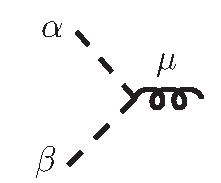
\includegraphics[width=13ex]{figures/Vssg}}}$ & $ \frac{i}{\sqrt{2}}(p_2-p_1)^\mu~ g^{\alpha\beta}_{[\mathcal{D}]}$ \\
    $\vcenter{\hbox{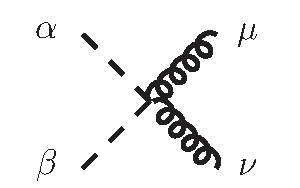
\includegraphics[width=15ex]{figures/Vssgg}}}$ & $ -\frac{i}{2}~g^{\mu\nu}_{[D_0]}~g^{\alpha\beta}_{[\mathcal{D}]}$ \\
    $\vcenter{\hbox{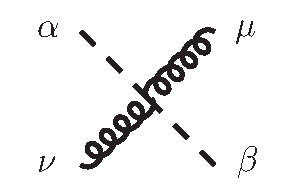
\includegraphics[width=15ex]{figures/Vsgsg}}}$ & $ i~g^{\mu\nu}_{[D_0]}~g^{\alpha\beta}_{[\mathcal{D}]}$ \\
  \end{tabular}
  \end{minipage}
  \quad
  \begin{minipage}[t]{0.5\textwidth}
  \begin{tabular}{cl}
    $\vcenter{\hbox{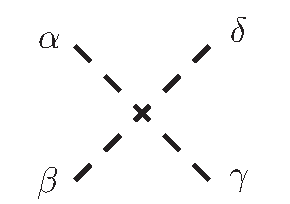
\includegraphics[width=15ex]{figures/Vssss1}}}$ &
      $
      \begin{aligned}
        i~g^{\alpha\gamma}_{[\mathcal{D}]} g^{\beta\delta}_{[\mathcal{D}]} - ~ & \\
                \frac{i}{2}~(g^{\alpha\beta}_{[\mathcal{D}]} g^{\gamma\delta}_{[\mathcal{D}]} & + g^{\alpha\delta}_{[\mathcal{D}]} g^{\beta\gamma}_{[\mathcal{D}]})
      \end{aligned}
      $ \\
        $\vcenter{\hbox{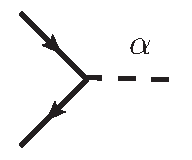
\includegraphics[width=11ex]{figures/VqqsR}}}$ & $- \frac{i}{\sqrt{2}}~\gamma^\star_{[D_0]} \gamma^\alpha_{[\mathcal{D}]}$ \\
        $\vcenter{\hbox{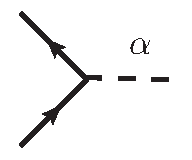
\includegraphics[width=11ex]{figures/VqqsL}}}$ & $ \frac{i}{\sqrt{2}}~\gamma^\star_{[D_0]} \gamma^\alpha_{[\mathcal{D}]}$ \\
  \end{tabular}
  \end{minipage}
  \caption{Color-ordered Feynman rules for vertices with scalars, which are introduced from dimensional reduction of gluons.}
  \label{tab:Ds-FeynRules}
\end{table}

To obtain the coefficients $\tilde{\mathcal{K}}_i$ in \cref{eq:ds-poly-alt} for an amplitude, we process each contributing  Feynman diagram with the following steps:
\begin{enumerate}
  \item Split all gluon lines in loops with \cref{eq:ds-split-metric} into a sum of $D_0$-dimensional gluon and a $\mathcal{D}$-dimensional gluon.
  \item Factorize all quark lines according to \cref{eq:ds-gamma}.
  \item Insert the Feynman rules from \cref{tab:Ds-FeynRules} and expand, keeping all $D_0$-dimensional objects untouched.
  \item Evaluate traces \eqref{eq:trace_d0}, and contract all $\mathcal{D}$-dimensional indices. 
     This replaces the $\mathcal{D}$-dimensional gluon by a scalar, and generates factors, which are polynomials in $\mathcal{D}$ with integer coefficients.
\end{enumerate}
An example of this procedure is given in \cref{fig:ds-example-diagram}.

\begin{figure}[ht]
  \newlength\diagramWidth
  \setlength{\diagramWidth}{18ex}
  \centering
  \begin{align*}
    \vcenter{\hbox{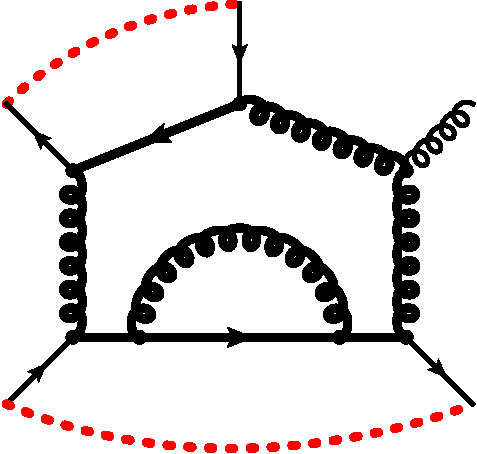
\includegraphics[width=\diagramWidth]{figures/Ds-example_B.pdf}}} \hspace{-10ex} & \hspace{15ex} = \hspace{6ex}
    \mathcal{D}^0 ~\cdot~ \vcenter{\hbox{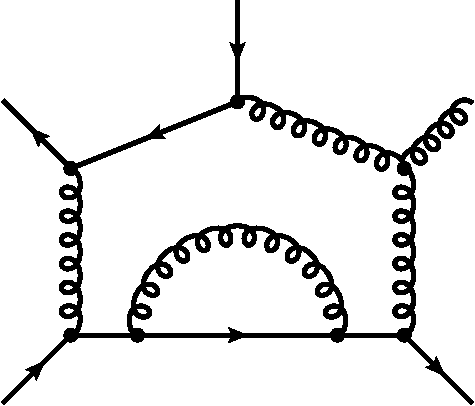
\includegraphics[width=\diagramWidth]{figures/Ds-example.pdf}}} \quad +\\
     & \mathcal{D}^1 ~\cdot~ \qty(~ 
    \vcenter{\hbox{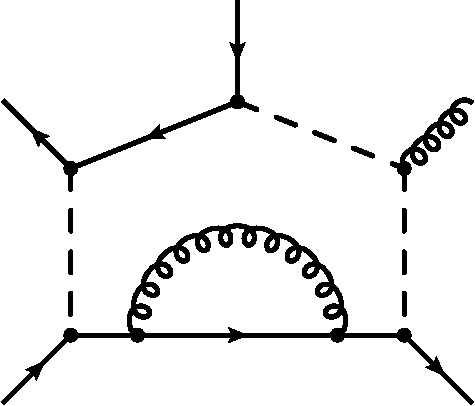
\includegraphics[width=\diagramWidth]{figures/Ds-example-1-1.pdf}}} \quad+\quad
    \vcenter{\hbox{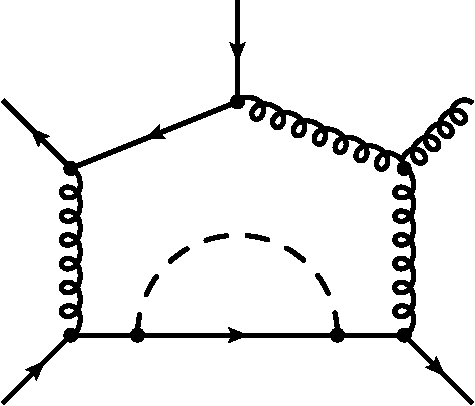
\includegraphics[width=\diagramWidth]{figures/Ds-example-1-2.pdf}}}
    ~) \quad +\\
     & \mathcal{D}^2 ~\cdot~ \quad \vcenter{\hbox{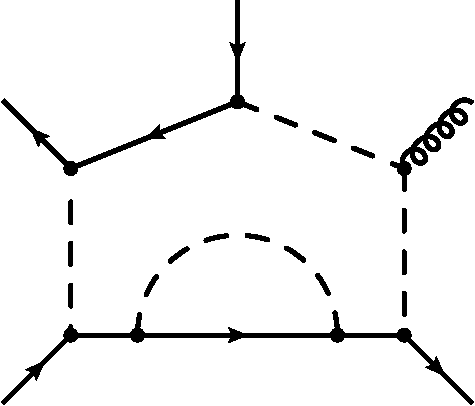
\includegraphics[width=\diagramWidth]{figures/Ds-example-2.pdf}}}
  \end{align*}
  \caption{Example of diagrams with scalar particles,
    representing the contributions to the coefficients of $\tilde{\mathcal{K}}_i$ in eq.~\eqref{eq:ds-poly-alt}.
    The thick lines in the diagram on the left-hand side represent particles in arbitrary $D_s$ dimensions.
    The (red) dashed represent the traces required for the projection in \cref{eq:dsm_4_projectors}.
    All particles on the right-hand side are $\mathcal{D}$-dimensional.}
  \label{fig:ds-example-diagram}
\end{figure}


Some comments are in order.
\begin{itemize}
  \item As a result of the algorithm presented above, all indices beyond $D_0$ are contracted.
    Taking the $\mathcal{D}$-dimensional traces, originated from the projections in \cref{eq:dsm_4_projectors}, was one of the prerequisites.
    These projections still need to be completed by evaluating the remaining traces over $(D_0-4)$-dimensional spinor indices,
    which can be done with explicit sums over the corresponding states, as in dimensional reconstruction.
  \item For two-loop amplitudes with no external fermions our method corresponds to the so called
six-dimensional helicity formalism \cite{Bern2011,Cheung:2009dc,Badger:2013gxa,Badger:2017jhb}.
From this point of view, our method can then be considered an extension thereof to amplitudes with fermions.
  \item Finally, although in this section we specialized to two-loop color-ordered QCD,
the generalization to different models and higher number of loops is straight-forward.
\end{itemize}



\subsection{Unitarity-Compatible Algorithm}
\label{dshel:sec:unitarity-compatible}

The algorithm for decomposition of amplitudes into $\mathcal{D}$ polynomials, 
described in the previous section, was formulated 
in terms of operating on individual Feynman diagrams.
In this regard, one might wonder if it can be employed together with
the numerical unitarity methods, where we evaluate
the products of tree amplitudes through off-shell recursion, 
as discussed in \cref{sec:evaluation_of_tree_amplitudes}.
Here we explain how this can be done.

Instead of decomposing Feynman diagrams, 
we need to decompose \emph{cut diagrams}, 
i.e.\ the diagrams with vertices being tree amplitudes 
(see \cref{sec:evaluation_of_cuts} for details).
To this end, we process each cut diagram as follows:
\begin{enumerate}
  \item Perform the dimensional reduction of each vertex $V_{[D_s]i}$ of the cut diagram by applying steps 1 to 3 of the algorithm from the previous section,
    taking into account that only the gluons originating from the cuts contribute non-trivially.
    As a result, each vertex is expanded into a linear combination of the form
    \begin{equation}
      V_{[D_s]i} = \sum_k T_k^{\vb*{\alpha}} \; \tilde{V}_{[D_0]i}^{(k)},
    \end{equation}
    where $T_k^{\vb*{\alpha}}$ are the tensor structures of spinor and vector indices $\vb*{\alpha} \in \mathsf{S}_{[\mathcal{D}]}$.
    The new vertices $\tilde{V}_{[D_0]}^{(i)}$ ``remember'' 
    the tensor structures they originated from by allowing the dimensionally-reduced particles 
    to couple only in the way consistent with the corresponding tensor structure.\footnote{
      In the off-shell recursion this can be implemented by simply removing all currents which do not match the expected couplings.
    }
    Note that no restrictions are imposed on external gluons.
    We illustrate this step by an example shown in \cref{fig:example_dstree}.

    %, in addition to the list of external $D_0$-dimensional particles,
    %are identified by a restriction on how 
  \item Evaluate traces \eqref{eq:trace_d0}, and contract all $\mathcal{D}$-dimensional indices
    to bring the cut diagram to the form
    \begin{equation}
      \prod_i V_{[D_s]i} ~\to~  \sum_k c_k(\mathcal{D}) \prod_i \tilde{V}_{[D_0]i}^{(k_i)},
    \end{equation}
    which is then trivially rearranged into \cref{eq:ds-poly-alt}.  We give an example in \cref{fig:example_ds_cut2}.
\end{enumerate}

In this way the analytic $D_s$ dependence of each cut diagram is determined.
The reduction with numerical unitarity techniques of \cref{chap:numunitarity} 
can therefore be applied directly to the coefficients $\tilde{\mathcal{K}}_i$, which are evaluated in $\mathsf{S}_{[D_0]}$.

\begin{figure}[ht]
  \centering
  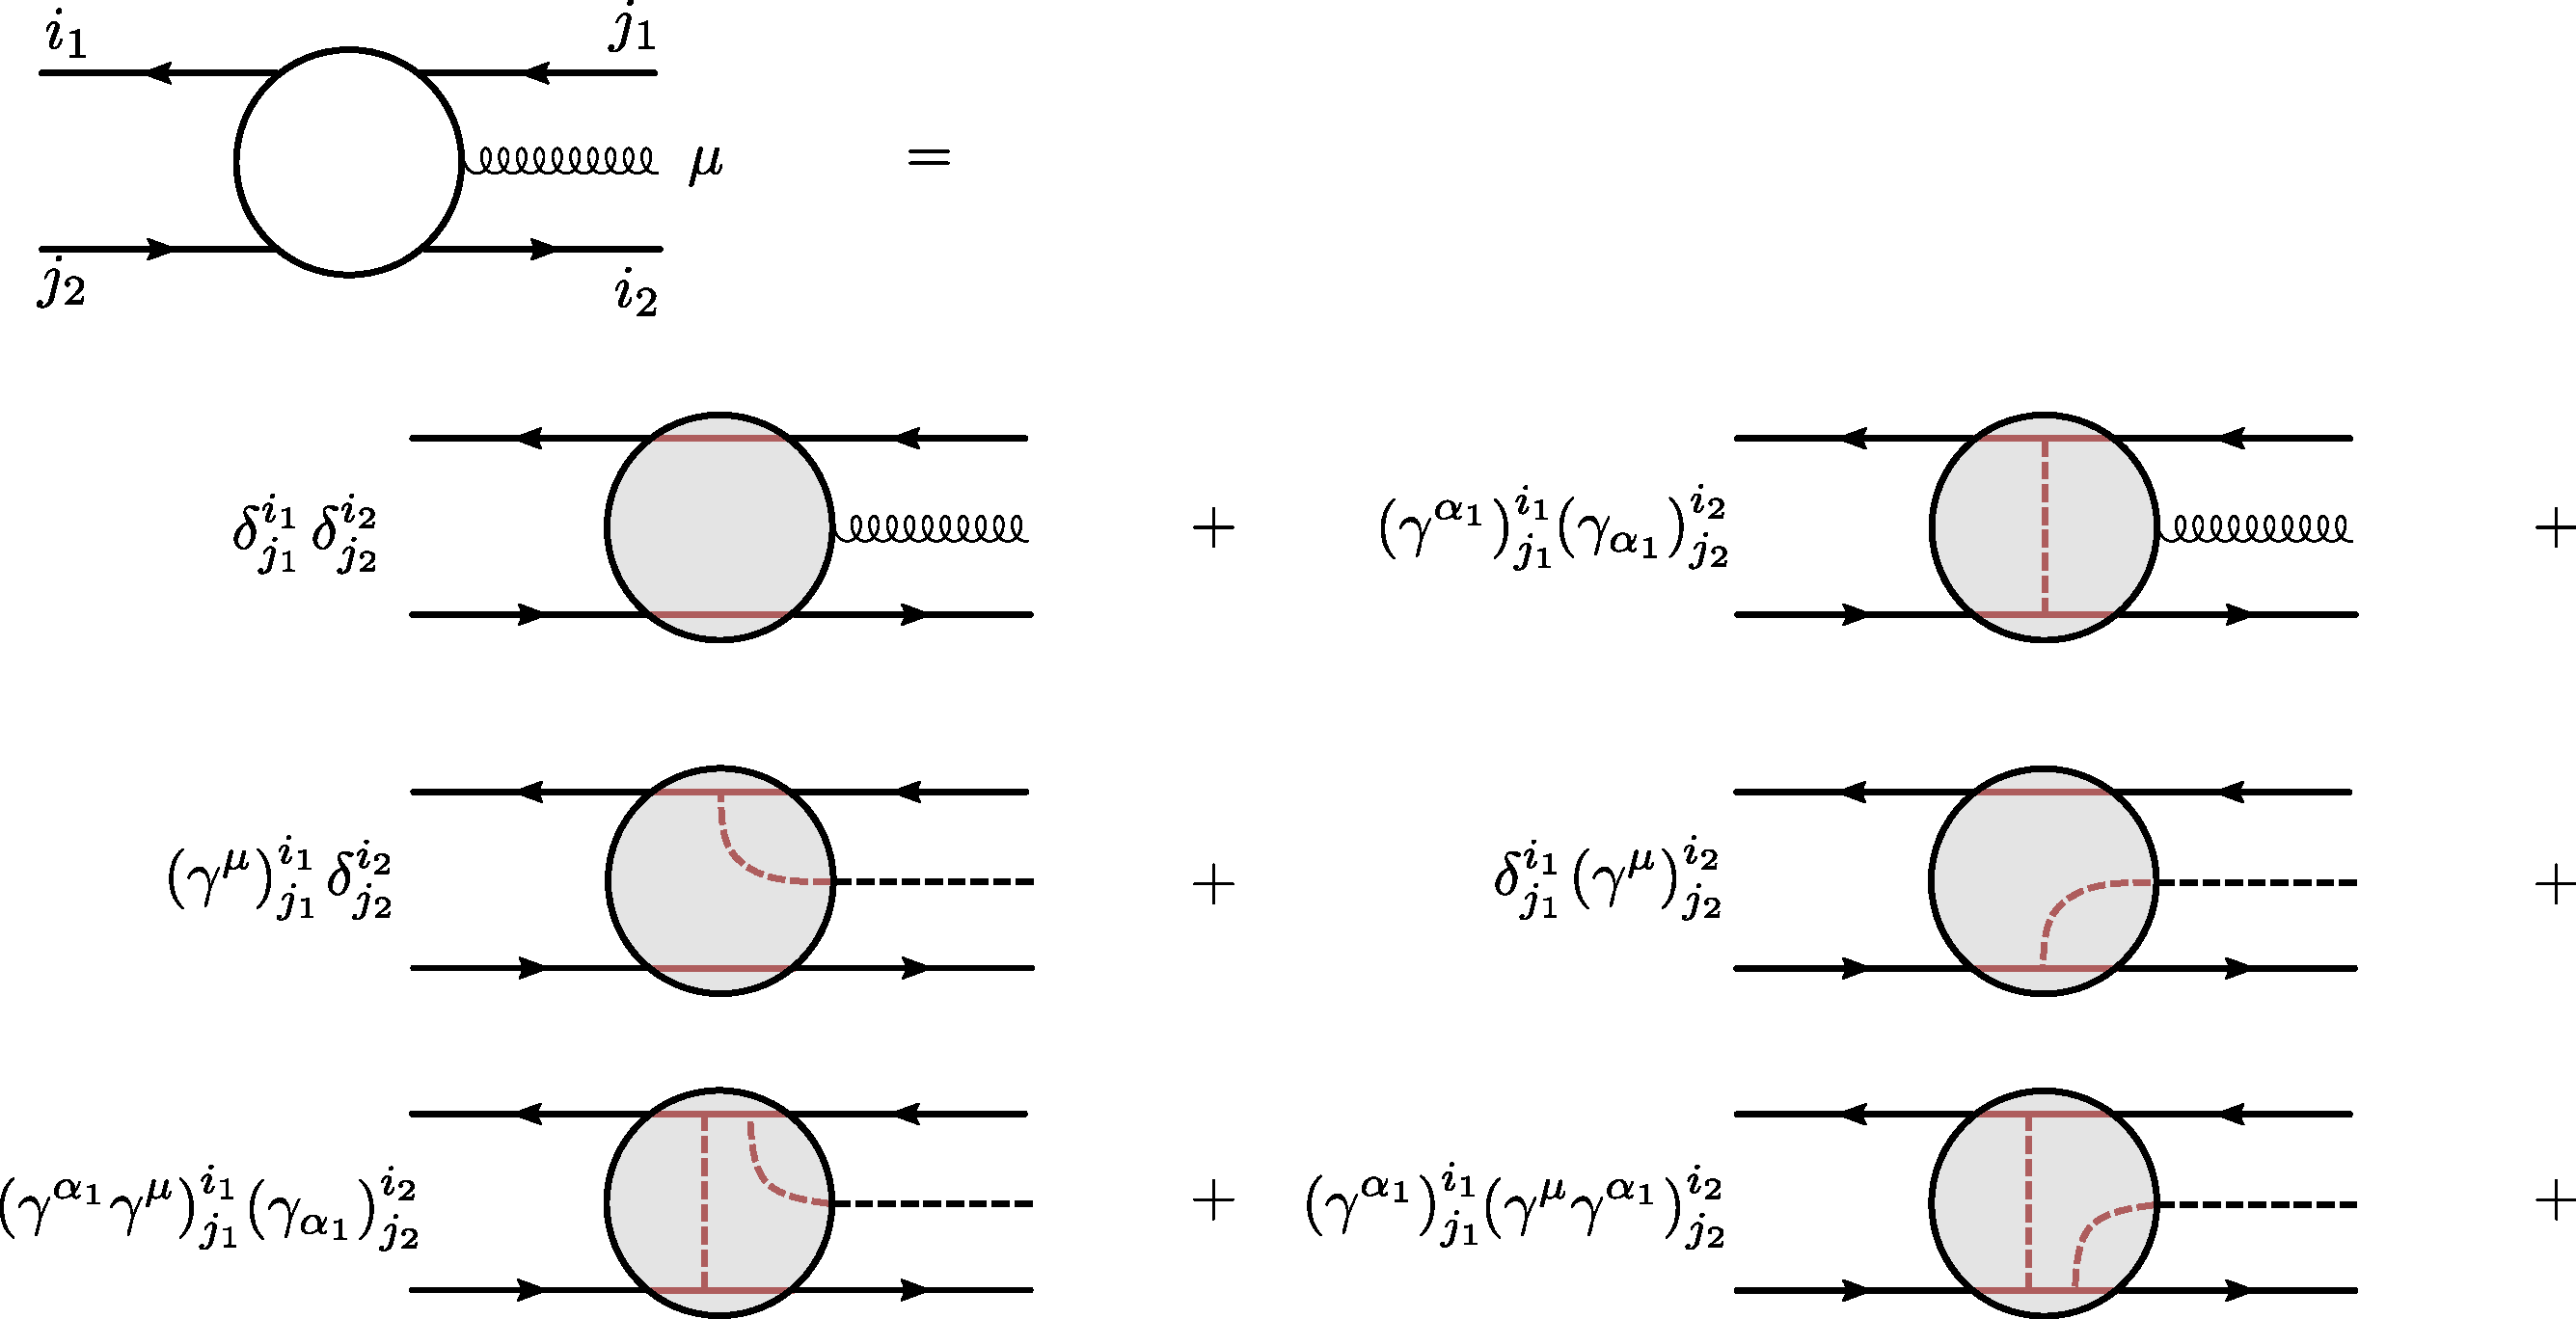
\includegraphics[width=0.9\textwidth]{example_dstree}
  \caption{An example of a dimensional reduction of a (color-ordered) 
    tree amplitude with particles in $D_s$ dimensions (on the left) into
    a linear combination of amplitudes in $D_0$ dimensions (on the right). 
    Only indices from $\mathsf{S}_{[\mathcal{D}]}$ are explicitly shown on the right.
    The shaded blobs specify subsets of diagrams with a particular coupling structure of the dimensionally-reduced particles, 
    which corresponds to the tensor structure in $\mathsf{S}_{[\mathcal{D}]}$.
  }
  \label{fig:example_dstree}
\end{figure}


\begin{figure}[ht]
  \centering
  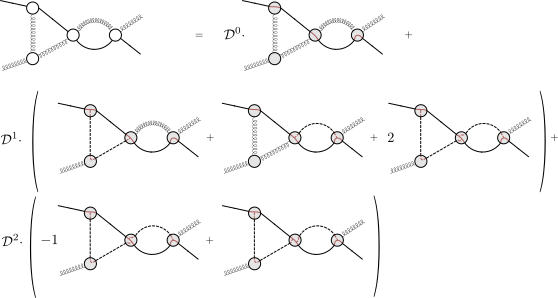
\includegraphics[width=1\textwidth]{example_ds_cut2}
  \caption{
    An example of the decomposition of a two-loop cut diagram in $D_s$ dimensions into coefficients $\tilde{\mathcal{K}}_i$ in \cref{eq:ds-poly-alt}.
    All diagrams on the right are in $D_0$ dimensions. The meaning of shaded blobs is as in \cref{fig:example_dstree}.
  }
  \label{fig:example_ds_cut2}
\end{figure}


%%-------------------------------------------------


%\chapter{Renormalization}
%\label{chap:renorm}
%In order to arrive at physical predictions, we need to
\textit{renormalize} QCD \ola s. Renormalization refers to the process of
connecting the initial Lagrangian parameters, so called bare
parameters, to physical quantities that can be measured in experiment. In a renormalizable theory, UV divergencies stemming from
virtual corrections drop out once the bare parameters are connected to
physical ones. The SM, and thus QCD, is a renormalizable theory \cite{tHooft:1971qjg,tHooft:1972tcz}.


We renormalize \ola s for processes involving massive quarks in a
mixed scheme. The strong coupling is renormalized in the
$\MSb$ scheme
and we apply a shift to decouple massive quark loops from the running of
$\alpha_s$. The wave-function and mass renormalization is done in the
on-shell scheme. The mass renormalization is performed at the
level of each color-ordered amplitude. Previously, we explicitly broke gauge invariance of the amplitudes by
removing external leg self-energy Feynman diagrams from tree
amplitudes that appeared in double cuts on \olb~topologies
(cf.~Sec.~\ref{sec:massivebubble}). After recombination with the corresponding mass counterterms, gauge
invariance of the \ola s is restored. The coupling renormalization and massive quark
decoupling as well as wave-function renormalization lead to a shift proportional to the tree amplitude. We provide all renormalization constants in FDH to
be consistent with the computation of the \ola s. 

Furthermore, in Sec.~\ref{sec:scaledep} we work out the correct \root~\cite{ROOT} \ntuple{} weights \cite{BH:Ntuples} for massive
one-loop amplitudes. Using \ntuple{} files allows for an efficient a-posteriori reevaluation of
matrix elements with different renormalization and factorization
scales as well as couplings and parton distribution functions.

\section{Multiplicative Renormalization}
\label{sec:stdrenorm}
We will briefly review the standard multiplicative renormalization
procedure (more details can be found in many textbooks \cite{PeskinS,Schwartz:2013pla,Bohm:2001yx}). In particular, we will see that mass counterterms have to
be computed at the level of each color-ordered amplitude whereas the
other renormalizations result in a shift proportional to the tree amplitude. We
reparameterize the bare parameters in the Lagrangian by 
\begin{align}
  \psi_0 & = \sqrt{Z_2}\psi_R, & A_0^\mu & =  \sqrt{Z_3} A_R^\mu, \\
m_0 & = Z_m m_R, & g_0 & = Z_g g_R, \notag
\end{align}
where $\psi_0$ is the bare fermion field, $A^\mu_0$ the bare QCD gauge field, $m_0$
the bare mass and $g_0$ the bare strong coupling. In perturbation
theory, we expand the renormalization constants $Z_i$ and get to first order
\begin{align}\label{eq:renconst}
  Z_2 & \equiv 1 + \delta_2, &  Z_3 &\equiv 1 + \delta_3,  \\
  Z_m & \equiv 1 + \delta_m, &  Z_g &\equiv 1 + \delta_g, \notag 
\end{align}
which leads to a split up of the Lagrangian. We get the
original Lagrangian in which bare parameters are replaced by
renormalized ones, and in addition, the so called \textit{counterterm}
Lagrangian that collects all terms in the renormalization constants $\delta_i$
and generates counterterm Feynman rules. The renormalization constants
multiplying the counterterm Feynman rules for QCD vertices are given by
\begin{align}\label{eq:vertqcdct}
\begin{split}
  Z_{3g}-1 = Z_3^{3/2}Z_g-1 &\equiv \frac{3}{2} \delta_3 +
  \delta_g, \\
  Z_{4g}-1 = Z_3^{4/2}Z_g^2 -1&\equiv  2\delta_3 + 2 \delta_g, \\
Z_{2q1g} -1= Z_2 Z_3^{1/2}Z_g -1 &\equiv  \delta_2 +
  \frac{1}{2}\delta_3 + \delta_g,
\end{split}
\end{align}
for the three- and four-valent gluon interaction $Z_{3g}$ and $Z_{4g}$
as well as the quark-gluon interaction $Z_{2q1g}$. The Feynman
rules for two-particle counterterms in Feynman gauge are given in Fig.~\ref{fig:qcdct}.
\begin{eqnarray*}
\begin{tikzpicture}[baseline=(m)]
  \begin{feynman}[inline=(m)]
    \vertex (m) at (0,0);
    \vertex (v1) at (1,0);
    \vertex (v2) at (2,0);
    \diagram* {
      (m)  -- [fermion,insertion={[size=8pt]0.99}] (v1) -- [fermion] (v2), 
    };
  \end{feynman}
\end{tikzpicture}
 & \qquad i\left((\slashed{p}-m_R)\delta_2 -
\delta_mm_R\right) &=P^q_{\text{ct}}(p)_{|\delta_2} +P^q_{\text{ct}}(p)_{|\delta_m}\\
\vspace{1cm}
\begin{tikzpicture}[baseline=(m)]
  \begin{feynman}[inline=(m)]
    \vertex (m) at (0,0);
    \vertex (v2) at (2,0);
    \diagram* {
      (m)  -- [gluon,insertion={[size=8pt]0.5}] (v2), 
    };
  \end{feynman}
\end{tikzpicture}& \qquad -ip^2\delta_3 g^{\mu\nu}&=P^{g,\mu\nu}_{\text{ct}}(p)\\
\end{eqnarray*}
\vspace{-1.5cm}
\captionedequationset{Feynman rules for QCD two-particle counterterms in Feynman gauge. The renormalization constants
  $\delta_i$ are defined in Eq.~\eqref{eq:renconst}.\label{fig:qcdct}} 
In principle, one has to compute all possible
counterterms as specified by the counterterm Feynman rules. However,
the simple counting exercise of Sec.~\ref{sec:renorm-shifts-prop} reveals that wave-function and coupling renormalization of QCD one-loop amplitudes lead to a
renormalization shift proportional to the tree. The remaining mass
renormalization counterterms have to be computed explicitly, as
spelled out in Sec.~\ref{sec:mrenorm}.

\section{Coupling and Wave-Function Renormalization}
\label{sec:renorm-prop-tree}

\subsection{Renormalization Shifts Proportional to Tree Amplitudes}
\label{sec:renorm-shifts-prop}

We first observe that the combination of two propagators of the QCD spectrum with a counterterm
insertion leads, for the parts independent of $\delta_m$, to the original propagator
multiplied by a renormalization constant. In particular, the counterterm
insertion on fermion propagators is given by
\begin{align}\label{eq:repropq}
\begin{split}
  P^q(p)P_{\text{ct}}^q(p)_{|\delta_2} P^q(p)& =  \frac{i(\slashed{p}+m_R)}{p^2-m_R^2}\left(i(\slashed{p}-m_R)\delta_2\right) \frac{i(\slashed{p}+m_R)}{p^2-m_R^2}\\
  &=-\delta_2\frac{i(\slashed{p}+m_R)}{p^2-m_R^2} = -\delta_2 P^q(p),
\end{split}
\end{align}
and that on gluon propagators by
\begin{align}\label{eq:repropg}
\begin{split}
  P^g_{\mu\nu}(p) P^{g,\nu\rho}_{\text{ct}} P^g_{\rho\sigma}(p)& =  \frac{-ig_{\mu\nu}}{p^2} \left(-ip^2\delta_3 g^{\nu\rho}\right)  \frac{-ig_{\rho\sigma}}{p^2}\\
  &=-\delta_3\frac{-ig_{\mu\sigma}}{p^2} = -\delta_3P^g_{\mu\sigma}(p).
\end{split}
\end{align}
It remains to show that the multiplicative renormalization factor of each Feynman diagram is
purely determined by the number and species of external particles. In
order to do so, we count vertices and
propagators of QCD tree amplitudes and multiply them with the corresponding
renormalization factors,
cf.~Eqs.~\eqref{eq:vertqcdct}-\eqref{eq:repropg}. We start with pure gluon amplitudes with $n$
external particles. For each Feynman diagram contributing to the
amplitude, we have
\begin{align}\label{eq:gvert}
  n = n_3 + 2 n_4 + 2,
\end{align}
where $n_3$ and $n_4$ are the number of three- and four-valent gluon
interactions. The number of gluon propagators $n_{\text{p,g}}$ is
related to the number of vertices by
\begin{align}\label{eq:gprop}
  n_{\text{p,g}} = n_3+ n_4 -1.
\end{align}
Therefore, the renormalization constants multiplying each Feynman
diagram are given by
\begin{align}
\begin{split}
  \text{R}(n,n_3,n_4,n_{\text{p,g}}) &= n_4 \left( 2\delta_3 + 2\delta_g \right) +n_3 \left(
    \frac{3}{2} \delta_3 + \delta_g \right)-n_{\text{p,g}} \delta_3\\
%&= n_4 \left( 2\delta_3 + 2\delta_g \right) +( n - 2 n_4 - 2) \left(
%    \frac{3}{2} \delta_3 + \delta_g \right)-(n - n_4 -3)\delta_3 \\
&= \frac{n}{2}\delta_3 +(n-2)\delta_g \equiv \text{R}(n),
\end{split}
\end{align}
where we used Eqs.~\eqref{eq:gvert} and \eqref{eq:gprop} as well as
the counterterm Feynman rules. Thus the renormalization constants
multiplying each Feynman diagram are only dependent on the number of
external legs. Wave-function
and coupling renormalization of pure gluon amplitudes are therefore
proportional to the corresponding tree
amplitude. 

We perform a similar counting exercise for processes involving both quarks and gluons. For a Feynman diagram of $n$ particles, with $N_g$ gluons, $N_q$ quarks, $n_3$ and $n_4$ gluon vertices and
$n_{\text{qg}}$ quark-gluon vertices, we get the relation
\begin{align}\label{eq:rqgen}
  n=N_g+N_q = n_3 + 2n_4 + n_{\text{qg}} +2.
\end{align}
The number of both gluon ($n_{\text{p,g}}$) and quark ($n_{\text{p,q}}$) propagators is given by
\begin{align}\label{eq:propqre}
  n_{\text{p,g}} &= n_3+n_4 + \left(\frac{N_q}{2} - 1\right), &   n_{\text{p,q}} &=
  n_{\text{qg}}-1- \left( \frac{N_q}{2} - 1\right).
\end{align}
The multiplicative renormalization factor $\text{R}(N_g,N_q,n_3,n_4,n_{\text{qg}},n_{\text{p,g}},n_{\text{p,q}})$ of each Feynman diagram with $N_g$ gluons and
$N_q$ quarks therefore reads
\begin{align}\label{eq:shiftfd}
\begin{split}
 \text{R}(\cdots) &= n_4 \left( 2\delta_3 + 2\delta_g \right) +n_3 \left(
    \frac{3}{2} \delta_3 + \delta_g \right)+n_{\text{qg}}\left(\delta_2+\frac{1}{2}\delta_3+\delta_g\right)-n_{\text{p,g}} \delta_3-n_{\text{p,q}} \delta_2\\
%&= n_4 \left( 2\delta_3 + 2\delta_g \right) +( n - 2 n_4 -n_{\text{qg}}+ (N_q-2)) \left(\frac{3}{2} \delta_3 +\delta_g \right)+n_{\text{qg}}(\delta_2+\frac{1}{2}\delta_3+\delta_g)\\
%&\phantom{m}-\left(n -n_4-n_{\text{qg}} + \frac{1}{2}(m - 2)\right) \delta_3-\left(n_{\text{qg}}-\frac{m}{2} \right) \delta_2\\
&=\frac{N_g}{2}\delta_3
+\frac{N_q}{2}\delta_2+\left(n-2\right)\delta_g \\
&\equiv \text{R}(N_g,N_q),
\end{split}
\end{align}
where we have used Eqs.~\eqref{eq:rqgen} and \eqref{eq:propqre} and
the counterterm Feynman rules. As above, the wave-function and coupling renormalization shift for
amplitudes containing quarks and gluons is proportional to a
tree amplitude.

\subsection{Renormalization Constants}
\subsubsection{Gluon Wave-Function Renormalization}
We renormalize the gluon wave function in the on-shell scheme. The
renormalization constant is fixed by the requirement that the residue
of the gluon propagator is one. As a side effect, we do not have
to calculate self-energy corrections on external gluon legs. The
renormalization constant in the on-shell scheme calculated in FDH is
given by
\begin{align}
Z_3^{\text{os}}=1+\delta_{3}=1-g_s^2c_\Gamma\frac{2}{3}\left(\frac{1}{\epsilon} +
  \log\left(\frac{\mu^2}{ m_{\text{os}}^2}\right)\right)+\mathcal{O}(g_s^4,\epsilon),
\end{align}
with a heavy quark with on-shell mass $m_{\text{os}}$ running in the
closed loop and the prefactor $\displaystyle
c_\Gamma=(4\pi)^{-(2-\epsilon)}\Gamma(1+\epsilon)\Gamma^2(1-\epsilon)/\Gamma(1-2\epsilon)$
appearing in all integrals and renormalization constants. As we saw
in Eq.~\eqref{eq:shiftfd}, each of the $N_g$ external gluons contributes a
factor of $\frac{1}{2}\delta_3$ and we get contributions from each
flavor in closed massive quark loops. Therefore the
renormalization shift to a \ola~involving $n$ particles and $N_g$ gluons is given by
\begin{align}
\begin{split}
  \text{R}_{\text{wf, gluon}} &= -g_s^{2}c_\Gamma
N_g\sum_{i=1}^{N_{hf}}\left(\frac{1}{3\epsilon} + 
  \frac{1}{3}\log\left(\frac{\mu^2}{ m_{i,\text{os}}^2}\right)\right)
\Ampt(1,\dots,n)\\
&=-g_s^{2}c_\Gamma
N_g \Delta_3 \Ampt(1,\dots,n),
\end{split}
\end{align}
where $N_{hf}$ denotes the number of heavy-quark flavors with mass $m_{i,\text{os}}$.
%There is no contribution from massless quarks to the gluon
%self-energy, since the corresponding integrals vanish in dimensional regularization.
\subsubsection{Massive Quark Wave-Function Renormalization}
 We use the on-shell scheme to renormalize the massive quark wave
 function and the renormalization constant in FDH is given by
\begin{align}
 Z_2^{\text{os}}=1+\delta_2&=1-g_s^2c_\Gamma C_F\left(\frac{3}{\epsilon}+3\log{\left(\frac{\mu^2}{m_{\text{os}}^2}\right)}+5\right)+\mathcal{O}(g_s^4,\epsilon),
\end{align}
with $C_F=\frac{N_C^2-1}{2N_C}$. 
%The constant $Z_2^{\text{os}}$ is fixed from requirements on the fermion propagator Eq.~\eqref{eq:osfermprop}.
%\begin{align}
% \lim_{p^2\rightarrow m^2_{\text{os}}}\left[\frac{i(\slashed{p}+m_{\text{os}})}{p^2-m^2_{\text{os}}}\left(1-{\hat\Sigma}_0(\slashed{p})-\frac{m_{\text{os}}(\slashed{p}+m_{\text{os}})\tilde{\Sigma}_1(\slashed{p})}{p^2-m_{\text{os}}^2}\right)u(p)\overset{!}{=}\frac{i(\slashed{p}+m_{\text{os}})}{p^2-m^2_{\text{os}}}u(p)\right],
%\end{align}
%which can be rephrased as
%\begin{align}
%  \hat\Sigma_0(m_{\text{os}}^2)+2m^2_{\text{os}}\tilde{\Sigma}^\prime_1(m_{\text{os}}^2)=0,
%\end{align}
%with the self-energies $\Sigma_i$ defined as in Sec.~\ref{sec:mrenorm} and
%$\Sigma^\prime(\slashed{p})=\pdv{\Sigma(\slashed{p})}{\slashed{p}}$. 
Each massive external fermion
contributes a factor of $\frac{1}{2}\delta_2$, see Eq.~\eqref{eq:shiftfd}. Therefore, the
renormalization shift to a \ola~involving $n$ particles including external massive quarks is given by
\begin{align}
\begin{split}
  \text{R}_{\text{wf, quark}} &= -g_s^{2}c_\Gamma
\sum_{i=1}^{N_{hf}}N_{Q_i}\frac{1}{2}C_F\left(\frac{3}{\epsilon}+3\log{\left(\frac{\mu^2}{m_{i,\text{os}}^2}\right)}+5\right)\Ampt(1,\dots,n)\\
&= -g_s^{2}c_\Gamma
\sum_{i=1}^{N_{hf}}N_{Q_i}\frac{\Delta_{2,i}}{2}\Ampt(1,\dots,n),
\end{split}
\end{align}
where $N_{hf}$ denotes the number of heavy-quark flavors and $N_{Q_i}$ the number of external quarks of flavor $i$ with on-shell mass $m_{i,\text{os}}$.

%See for example:\\
%KST, \url{https://arxiv.org/pdf/hep-ph/9305239.pdf}\\
%\url{https://arxiv.org/pdf/0807.4424.pdf}\\
%\url{https://arxiv.org/pdf/hep-ph/9310301.pdf}\\
%Weinzierl, \url{https://arxiv.org/pdf/hep-ph/0207055.pdf}

\subsubsection{Coupling Renormalization}
The coupling renormalization constant is fixed by a
calculation of the
vacuum polarization. We use the $\MSb$ scheme, where the
renormalization constant for the coupling computed in FDH is given by
\begin{align}
 Z_g^{\MSb}=1+\delta_g=1-g_s^2c_\Gamma\frac{1}{2}\left(\frac{11\NC-2(\NF+N_{hf})}{3\epsilon}-\frac{\NC}{3}\right)
 + \mathcal{O}(\epsilon,g_s^4),
\end{align}
with $\NF$ denoting the number of light and $N_{hf}$ the
number of heavy-quark flavors. The finite shift $\frac{\NC}{3}$ stems
from the translation of the gauge coupling from standard $\MSb$ to the
FDH variant. As we saw in Eq.~\eqref{eq:shiftfd}, each power $N_{g_s}$ of the strong coupling $g_s$ contributes to the renormalization shift
\begin{align}
\begin{split}
 \text{R}_{\text{coupling}} &= -g_s^{2}c_\Gamma \frac{N_{g_s}}{2}
 \left(\frac{11\NC-2(\NF+N_{hf})}{3\epsilon}-\frac{\NC}{3}\right)\Ampt(1,\dots,n)\\
 &= -g_s^{2}c_\Gamma N_{\alps} \Delta_{\alps}\Ampt(1,\dots,n).
\end{split}
\end{align}
For pure QCD amplitudes, the power of $g_s$ is given by
$N_{g_s}=n-2$ and that of $\alps$ by $N_{\alps}=N_{g_s}/2$. For amplitudes
involving \ew~gauge bosons, the counting is reduced accordingly.
\subsubsection{Heavy-Quark Decoupling}
We work in the decoupling scheme \cite{Collins1978a}. That is, we require
that heavy quarks decouple from the running of
$\alpha_s$ at energies $E\ll m_{hf}$. Consequently, the appropriate $\MSb$ coefficients for the
running of $\alpha_s$ should be the same as in absence of the heavy
quarks. Therefore, diagrams with a heavy quark loop
are subtracted at zero momentum transfer and the decoupling shift for an
$n$-particle amplitude with $\frac{n-2}{2}$ powers of the strong
coupling $\alps$ and $N_{hf}$ decoupled heavy-quark flavors is
given by
\begin{align}
\begin{split}
\text{R}_{\text{decoupling}}&= g_s^{2}c_\Gamma
N_{\alps}\sum_{i=1}^{N_{hf}}
\frac{2}{3}\log(\frac{\mu^2}{m_{i,\text{os}}}) \Ampt(1,\dots,n)\\
&= -g_s^{2}c_\Gamma N_{\alps}\sum_{i=1}^{N_{hf}}
\Delta_i\Ampt(1,\dots,n),
\end{split}
\end{align}
where the sum runs over heavy quark flavors $N_{hf}$ and $N_{\alps}$ denotes the power of the coupling $\alps$. For processes involving \ew~gauge bosons, the counting is
reduced accordingly.
%\url{http://lanl.arxiv.org/pdf/hep-ph/0508242}
%\url{https://ac.els-cdn.com/0550321382900384/1-s2.0-0550321382900384-main.pdf?_tid=3fc95d9e-a468-11e7-b8d4-00000aacb362&acdnat=1506615511_0873854316f0722bef4a45c5ee57e85d}

\section{Mass Renormalization}
\label{sec:mrenorm}
For processes involving massive quarks, we need to renormalize the
bare mass parameter. Its renormalization cannot be represented
as a contribution proportional to the tree amplitude. For convenience we combine the computation of these
contributions with the bubble diagrams. We explicitly
compute mass-counterterm contributions using a dedicated recursive
tree-like computation at the level of primitive loop amplitudes. The only source to the $\delta_m$ counterterm is the two-particle QCD counterterm interaction, cf.~Fig.~\ref{fig:qcdct} and Eq.~\eqref{eq:vertqcdct} 
\begin{align}\label{eq:fermionpropins}
  P^q_{\text{ct}}(p)_{|\delta_m} = -im_R \delta_m.
\end{align}
For double cut topologies with a gluon and a massive quark
cut line, the mass counterterm is computed by replacing the two cut lines of the bubble with fermion propagators and the above insertion of
Eq.~\eqref{eq:fermionpropins} as shown in Fig.~\ref{fig:massct}. The counterterm for a double cut topology
with legs $1_g,\dots,j_{\bar{q}}$ joining in vertex one and
$(j+1)_g,\dots,n_q$ in vertex two is thus computed by
\begin{align}
  \text{CT}_{1_g,\dots,j_{\bar{q}};(j+1)_g,\dots,n_q} =
  Q(1_g,\dots,j_{\bar{q}}) P^q_{\text{ct}}(P_{1j})_{|\delta_m} \bar{Q}((j+1)_g,\dots,n_q),
\end{align}
where we denoted the momentum sum $P_{ij}=\sum_{k=i}^jp_k$ and $Q$ and
$\bar{Q}$ denote quark and anti-quark Berends-Giele currents respectively. By adding these
counterterms to each color-ordered \ola, gauge invariance is
restored at the level of primitive amplitudes, after initially being broken by the removal of external leg self-energy insertions in \olb~cuts, cf.~Sec.~\ref{sec:massivebubble}.
\begin{equation*}
\begin{tikzpicture}[baseline=(m1)]
  \def\leglength{1}
  \def\blobpos{2.5}
  \def\cutshift{0.3}
  \def\cutlength{1.0}

  %The double cut lines
  \pgfmathsetmacro\vertcut{(\blobpos-1)/2+1}
  \draw[very thick] (\vertcut,\cutshift) -- (\vertcut,\cutshift+\cutlength);
  \draw[very thick] (\vertcut,-\cutshift) -- (\vertcut,-\cutshift-\cutlength);

  %\node at (-0.3,0) {\(1_{\bar{q}}\)};
  \begin{feynman}[inline=(m1)]
    \vertex[blob] (m) at (\blobpos, 0) {};
    \vertex[blob] (m1) at (1, 0){};
    \vertex (i) at (0, 0){\(\vdots\)};
    \vertex (i1) at (0, \leglength){\(j_{\bar{q}}\)};
    \vertex (i2) at (0, -\leglength){\(1_g\)};
    \vertex (a) at (\blobpos+\leglength,0){\(\vdots\)};
    \vertex (b) at (\blobpos+ \leglength,\leglength){\( (j+1)_{g} \)};
    \vertex (c) at (\blobpos+ \leglength,- \leglength){\(n_{q}\)};
    \diagram* {
     (m1) -- [gluon, half left,out=90,in=90] (m)
       -- [half left, thick,out=85,in=95] (m1),
       (m) -- [gluon] (b),
       (m1) -- [anti fermion] (i1),
       (m1) -- [gluon] (i2),
      (m) -- [fermion,  thick] (c),
    };
  \end{feynman}
\end{tikzpicture}
\hspace{0.5cm}\longrightarrow\hspace{0.5cm}
\begin{tikzpicture}[baseline=(m1)]
  \def\leglength{1}
  \def\blobpos{3.5}
  \def\cutshift{0.3}
  \def\cutlength{1.0}

  %\node at (-0.3,0) {\(1_{\bar{q}}\)};
  \begin{feynman}[inline=(m1)]
    \vertex[blob] (m) at (\blobpos, 0) {};
    \vertex[blob] (m1) at (1, 0){};
    \vertex (mi) at (2.25, 0);
    \vertex (i) at (0, 0){\(\vdots\)};
    \vertex (i1) at (0, \leglength){\(j_{\bar{q}}\)};
    \vertex (i2) at (0, -\leglength){\(1_g\)};
    \vertex (a) at (\blobpos+\leglength,0){\(\vdots\)};
    \vertex (b) at (\blobpos+ \leglength,\leglength){\( (j+1)_{g} \)};
    \vertex (c) at (\blobpos+ \leglength,- \leglength){\(n_{q}\)};
    \diagram* {
      (m1) -- [fermion,insertion={[size=8pt]0.99}] (mi)   -- [fermion] (m),
       (m) -- [gluon] (b),
       (m1) -- [anti fermion] (i1),
       (m1) -- [gluon] (i2),
      (m) -- [fermion,  thick] (c),
    };
  \end{feynman}
\end{tikzpicture}
\end{equation*}
\vspace{-1.2cm}
\captionedequationset{Generation of mass counterterms. For double cut
  topologies with a gluon and fermion cut line, we compute the
  corresponding counterterm by joining the two currents
  $Q(1_g,\dots,j_{\bar{q}})$ and $\bar{Q}((j+1)_g,\dots,n_q)$ with the
  fermion two-particle counterterm interaction.\label{fig:massct}} 


We renormalize the mass in the \textit{on-shell scheme}. The renormalization
constant $Z_m$, computed in Feynman gauge and expressed in FDH is given by
\begin{align}\label{eq:rcm}
\begin{split}
  Z_m^{\text{os}}=1+\delta_m&=1-C_Fg_s^2c_\Gamma
  \left(\frac{\mu^2}{m_{\text{os}}^2}\right)^\epsilon
  \left(\frac{3}{\epsilon}+5\right)+\mathcal{O}(g_s^4)\\
&=1-C_Fg_s^2c_\Gamma \left(\frac{3}{\epsilon}+3\log{\left(\frac{\mu^2}{m_{\text{os}}^2}\right)}+5\right)+\mathcal{O}(g_s^4,\epsilon).
\end{split}
\end{align}
The color factor $C_F$ evaluates to $C_F=1$ if we compute the counter
terms for color-ordered particles. In the
on-shell scheme, the renormalization constant
$Z_m^{\text{os}}$ is fixed such that the pole of the
propagator is described by the renormalized mass
$m_{\text{os}}$, thereby fixing the finite terms. 

%Summing up the one-particle irreducible contributions
%to the fermion propagator up to first order, we get
%\begin{align}\label{eq:osfermprop}
%\begin{split}
%  \hat{P}^q(p)&=\frac{i(\slashed{p}+m_R)}{p^2-m^2_R}\left(1-\frac{(\slashed{p}+m_R)\hat\Sigma(\slashed{p})}{p^2-m_R^2}\right)\\
%&=\frac{i(\slashed{p}+m_R)}{p^2-m^2_R}\left(1-{\hat\Sigma}_0(\slashed{p})-\frac{m_R(\slashed{p}+m_R)\tilde{\Sigma}_1(\slashed{p})}{p^2-m_R^2}\right),
%\end{split}
%\end{align}
%where we denote renormalized quantities with a hat. The renormalized
%self-energy $\hat\Sigma(\slashed{p})$ can be split into vectorial and scalar part
%according to $\hat\Sigma(\slashed{p})=\slashed{p}{\hat\Sigma}_0(\slashed{p})+m{\hat\Sigma}_1(\slashed{p})$ and the sum of the
%parts is denoted by
%$\tilde{\Sigma}_1(\slashed{p})={\hat\Sigma}_0(\slashed{p})+{\hat\Sigma}_1(\slashed{p})$. If we then require
%to have a simple pole in Eq.~\eqref{eq:osfermprop} for $p^2\rightarrow m_R\equiv m_{\text{os}}$, we obtain the renormalization condition
%\begin{align}\label{eq:rnc1}
%  \lim_{p^2\rightarrow m^2_{\text{os}}}\tilde{\Sigma}_1(p^2) = \tilde{\Sigma}_1(m_{\text{os}}^2)  = 0.
%\end{align}
%The sum of renormalized self-energies
%${\tilde\Sigma}_1(m_{\text{os}}^2)$ written in terms of unrenormalized
%self-energies is given by
%\begin{align}
%\begin{split}
%  \tilde{\Sigma}_1(m_{\text{os}}^2) &=
%  {\hat{\Sigma}}_0(m_{\text{os}}^2)+{\hat \Sigma}_1(m_{\text{os}}^2) \\
%&=  {\Sigma}_0(m_{\text{os}}^2)+{\Sigma}_1(m_{\text{os}}^2)-\delta_{m}^{\text{os}}=0,
%\end{split}
%\end{align}
%which fixes the finite part of $Z_m^{os}\equiv
%1+\delta_{m}^{\text{os}}$. It evaluates in FDH to Eq.~\eqref{eq:rcm}, given the expressions for the unrenormalized quark
%self-energies in QCD.



%\subsection{$\gamma_5$ renormalization}
%In the HV scheme we do have a finite shift for $gamma_5$.
%\begin{align}
%  \gamma^\mu\gamma_5 \rightarrow   \frac{1}{2} Z_{axial}(\gamma^\mu\gamma_5 -  \gamma_5\gamma^\mu)\notag
%\end{align}
%with $Z_{axial}=1-2C_F 1_{HV}$\\
%\url{https://arxiv.org/pdf/hep-ph/9903380.pdf}

\section{Summary of Renormalization}
\label{sec:summary}
In summary, we renormalize \ola s in a mixed scheme. For external states we use the on-shell
scheme and the gluon wave-function renormalization receives contributions from all
active heavy quark flavors. We renormalize the mass in the on-shell scheme
and compute mass renormalization counterterms
explicitly at the level of each color-ordered amplitude. The QCD coupling is renormalized in $\MSb$, where we decouple massive quarks from the
running of $\alpha_s$. The renormalized \ola~is obtained by combining all tree-like renormalization shifts with the mass renormalized \ola
\begin{align}
\begin{split}
  \Amp_{(ren)}&=
  \Amp_{(mass\
    ren)}+\text{R}_{\text{wf,quark}}+\text{R}_{\text{wf,gluon}}+\text{R}_{\text{coupling}}+\text{R}_{\text{decoupling}}\\
&= \Amp_{(mass\
    ren)}-g_s^2 c_\Gamma \left( \sum_{i=1}^{N_{hf}} N_{Q_i} \frac{\Delta_{2,i}}{2} + N_{g}\Delta_3 +
    N_{\alps}\left(\Delta_{\alps} + \sum_{i=1}^{N_{hf}}\Delta_i\right) \right)  \mathcal{A}^{\text{tree}},
\end{split}
\end{align}
where $N_{hf}$ denotes the number of heavy flavors, $N_{Q_i}$ the number of external heavy quarks of flavor $i$, $N_g$ the number of external
gluons and $N_{\alps}$ the power of $\alps$ (at Born level) . The
renormalization constants in the FDH scheme are summarized in Table \ref{tab:renorm}.
\begin{table}[h]
  \caption{Renormalization constants used in this thesis. Here $\mu$ is the renormalization
  scale, $m_{i}$ are the masses for heavy quarks, $\NF$ is the number of light flavors,
  $N_{hf}$ the number of heavy flavors, and $\NC$ the number of colors.
  A common factor of $-g_s^2 c_\Gamma$ has been factored out.}
      \vskip 4mm
  \centering
    \begin{tabularx}{\textwidth}{lcll}
      \hline\hline
      \noalign{\vskip 4mm}
      \textbf{Renormalization} & \textbf{Scheme} & \textbf{Constant}\\
      \noalign{\vskip 3mm}
      \hline
      \noalign{\vskip 2mm}
      %\rule{0pt}{1ex}\\
    %\small
      %\toprule
      Heavy-quark wave function   & on-shell & $\displaystyle
      \Delta_{2,i} ~=~ \frac{\NC^2-1}{2\NC} \left( \frac{3}{\epsilon}
        + 3 \log{\frac{\mu^2}{m_i^2} + 5} \right)$\\
      \noalign{\vskip 1mm}
      Light-quark wave function   & on-shell & 0\qquad(UV+IR
      cancellation) \\
      \noalign{\vskip 3mm}
      Quark mass            & on-shell & $\displaystyle \Delta_{m_i}
      ~=~ \Delta_{2,i}\quad\text{}$\\
      \noalign{\vskip 1mm}
      Gluon wave function   & on-shell & $\displaystyle \Delta_3 ~=~ \sum_{i=1}^{N_{hf}}\left(\frac{1}{3 \epsilon} +
      \frac{1}{3}\log{\frac{\mu^2}{m_i^2}}\right)$\\
      \noalign{\vskip 1mm}
      QCD coupling & $\MSb$ & $\displaystyle \Delta_{\alps} ~=~  \frac{1}{\epsilon} \left( \frac{11}{3}\NC - \frac{2}{3}(\NF+N_{hf}) \right) - \frac{\NC}{3}$\\
      \noalign{\vskip 2mm}
      \hline
      \noalign{\vskip 2mm}
      Decoupling shift & --- & $\displaystyle     \Delta_i ~=~-
      \frac{2}{3}\log{\frac{\mu^2}{m_i^2}} $\\
      \noalign{\vskip 1mm}
      \hline\hline
    \end{tabularx}
  \label{tab:renorm}
\end{table}

\section{Scheme Shift From FDH to 't Hooft-Veltman}
\label{sec:schemeshift}
We use the FDH variant of dimensional regularization in intermediate steps to
regularize UV and IR divergences. At the end we convert the renormalized
amplitude to the HV scheme~\cite{tHooft:1972tcz} which is often more convenient for comparisons and interfacing with Monte-Carlo generators. The conversion of a renormalized \ola~$\Amp_{(ren)}$ is performed by a finite shift, see
e.g.\ \cite{Signer:2008va}
\begin{align}
  \mathcal{A}_{(ren)}^{\text{1-loop,HV}} =
  \mathcal{A}_{(ren)}^{\text{1-loop,FDH}} - g_s^{2}c_\Gamma\left(N_g\frac{\NC}{6}+N_q\frac{\NC^2-1}{4\NC}\right)\Ampt,
\end{align}
where $N_g$ denotes the number of gluons and $N_q$ the number of light
quarks in the respective amplitude.



\section{Scale Variation Using \Ntuple{} Data}
\label{sec:scaledep}

We provide NLO results in the form of \root~\cite{ROOT} \ntuple{} files \cite{BH:Ntuples}. The \ntuple{} files allow to reevaluate
generic IR-safe observables with different renormalization and
factorization scales as well as different PDFs. They store the relevant information to
reevaluate observables without recomputing the short-distance matrix
elements, which is possible due to the particular simple form of the parts of the virtual matrix element that depend on $\mu_R$. This possibility for a-posteriori variations of scales and PDFs
make the efficient estimation of uncertainties associated to NLO
predictions possible. 

In this section, we analyze the dependence of virtual cross sections on the unphysical renormalization scale. We neglect the implicit dependence
via the strong coupling for this discussion, since it amounts to a global prefactor and can be
treated as described in \cite{BH:Ntuples}. In particular, we identfiy additional
renormalization terms with $\mu_R$ dependence which are present in calculations with massive external particles and have to be considered in order to supply the correct data for \ntuple{} files.

The dependence of the virtual cross section on the unphysical scale
$\mu_R$ is introduced in
dimensional regularization to enforce a mass dimension of one for the
gauge 
couplings $g\rightarrow \mu_R^{\epsilon}g$. As a consequence, there is
an explicit dependence on $\mu_R$ in virtual NLO matrix elements. We can write an unrenormalized, one-loop
amplitude, with couplings stripped off, as
\begin{align}\label{eq:mudep}
  \Amp(\mu_R) =  \tilde{\mu}_R^{2\epsilon}\left[\frac{a_{2}}{\epsilon^2}+\frac{a_{1}}{\epsilon}
  + a_0\right],
\end{align}
where we use the dimensionless scale $\tilde{\mu}_R =
\frac{\mu_R}{\text{GeV}}$ to simplify the argument in the following. We generically have ratios of
renormalization scale $\mu_R$ and involved physical scales, from which
we build dimensionless quantities by
\begin{align}
 \left(\frac{\mu_R}{s}\right)^{2\epsilon} =\tilde{\mu}_R^{2\epsilon}\left(\frac{\text{GeV}}{s}\right)^{2\epsilon}.
\end{align}
Note, that Eq.~\eqref{eq:mudep} is valid for
any number of involved physical scales.
%\footnote{Assume we had two scales, the initial expression expression
%would be $ \sigma_V =
%(\frac{\mu_R}{sc_1})^{2\epsilon}\left[\frac{b_{2}}{\epsilon^2}+\frac{b_{1}}{\epsilon}
%+ b_0\right]+
%(\frac{\mu_R}{sc_2})^{2\epsilon}\left[\frac{c_{2}}{\epsilon^2}+\frac{c_{1}}{\epsilon}
%+ c_0\right]$. After identifying two identical dimensionless scales,
%we see that a redefinition of the parameters $b_i$ and $c_i$ leads to
%the form in Eq.~\eqref{eq:mudep}.}. 
We then expand $\left(\tilde{\mu}_R\right)^{2\epsilon}$ and obtain
\begin{align}
   \tilde{\mu}_R^{2\epsilon} = 1 +
   \log(\murt)\epsilon+\frac{1}{2}\log(\murt)^2\epsilon^2
   + \mathcal{O}(\epsilon^3),
\end{align}
such that the explicit $\tilde \mu_R$ dependence of
Eq.~\eqref{eq:mudep} becomes transparent
\begin{align}\label{eq:unrenam}
    \Amp(\mu_R)  = \left[\frac{a_{2}}{\epsilon^2}+\frac{a_{1}+a_{2}\log(\murt)}{\epsilon}
  + a_0+a_{1}\log(\murt)+\frac{1}{2}a_{2}\log(\murt)^2\right].
\end{align}
This formula contains double and single poles due to infrared
divergencies as well as single poles due to ultraviolet
divergencies. The difference of the finite part of the amplitude computed at two distinct scales $\mu_{R,1}$ and $\mu_{R,2}$ is then given by
\begin{align}\label{eq:extrapolscale}
\begin{split}
\Amp_{|\epsilon^{0}}({\mu}_{R,2}) -\Amp_{|\epsilon^{0}}({\mu}_{R,1})
  &=  a_1\log(\frac{\tilde{\mu}_{R,2}^2}{\tilde{\mu}_{R,1}^2})
+\frac{1}{2} a_2 \left[
    \log(\tilde{\mu}_{R,2}^2)^2-
    \log(\tilde{\mu}_{R,1}^2)^2\right]\\
&=  \left[a_1+a_2\log(\tilde{\mu}_{R,1}^2)\right]\log(\frac{\tilde{\mu}_{R,2}^2}{\tilde{\mu}_{R,1}^2})
+\frac{1}{2} a_2
\log(\frac{\tilde{\mu}_{R,2}^2}{\tilde{\mu}_{R,1}^2})^2,
\end{split}
\end{align}
which we can parameterize in terms of the weights $w_1$ and $w_2$
\begin{align}\label{eq:unrenweights}
  w_1 &\equiv a_{1}+a_2
  \log(\tilde{\mu}_{R,1}^2)=\Amp_{|\epsilon^{-1}},& w_2 &\equiv a_{2} = \Amp_{|\epsilon^{-2}}. 
\end{align}
The above parameterization has the advantage, that only ratios of
renormalization scales have to be considered and no explicit
dimensionless scales have to be constructed. The finite part of an unrenormalized \ola~at scale
$\tilde{\mu}_{R,2}$ can thus be extrapolated from that at scale
$\tilde{\mu}_{R,1}$ by adding the terms in Eq.~\eqref{eq:extrapolscale}
\begin{align}\label{eq:extrapolscale2}
\begin{split}
  \Amp_{|\epsilon^{0}}({\mu}_{R,2})   &= \Amp_{|\epsilon^{0}}({\mu}_{R,1}) +
  w_1\log(\frac{\tilde{\mu}_{R,2}^2}{\tilde{\mu}_{R,1}^2})+
\frac{1}{2} w_2
\log(\frac{\tilde{\mu}_{R,2}^2}{\tilde{\mu}_{R,1}^2})^2.
\end{split}
\end{align}
The above considerations are independent
of whether the involved particles are massive or not. In the
renormalization procedure, see the previous sections, additional
sources of $\mu_R$ dependence are introduced. Whereas mass and wave-function
renormalization lead to terms in which the logarithmic dependence in
the finite part has the same prefactor as the single pole, the shift
due to charge renormalization has no dependence on $\mu_R$ but
contributes to the single pole. Its
schematic contributions in an $\epsilon$ expansion
$(\epsilon^{-1},\epsilon^0)$ is given by
\begin{align}
   \text{R}_{\text{charge}} & = (a_{1,c},a_{0,c}),
\end{align} 
with coefficients $a_i$ that do not contain any logarithms. The decoupling
shift for massive quarks however has finite logarithms but no contribution
to the single pole
\begin{align}
   \text{R}_{\text{decoupling}} & = (0,a_{0,dec}\log(\murt)).
\end{align}
The weight $w_1$ should correctly parameterize simple logs of $\mu_R$ in
the finite part. To account for the absence of $\mu_R$ dependence in the charge renormalization and the fact that the decoupling shift
does not have a single-pole contribution, the weights for renormalized
amplitudes are defined as 
\begin{align}\label{eq:reweights}
 w_1 &=\Ampr_{|\epsilon^{-1}} -a_{1,c}+ a_{0,dec}, &  w_2 &= \Ampr_{|\epsilon^{-2}}.
\end{align}
With these weights, one can use Eq.~\eqref{eq:extrapolscale} to
extrapolate the virtual cross section to different values of $\mu_R$
for processes involving massive particles.

We provide the weights in Eq.~\eqref{eq:reweights} for each
phase space point together with the finite part of the matrix element squared. They
are stored in \ntuple{} files alongside information like the phase-space
point, the involved partons, the factorization and renormalization
scales, the Bjorken-x and the corresponding PDF
weights. We make extensive use of a-posteriori scale variations in the phenomenological
results presented in the following Chapters \ref{chap:wbb_intro}-\ref{chap:vjet_result}.


%%-------------------------------------------------

%\newpage
%\phantomsection
%\thispagestyle{empty}
%\vspace*{60 mm}
\begin{center}
{\Huge{\textbf{Part 2:}}}\\
\vspace*{5 mm}
{\Huge{\textbf{\texorpdfstring{$Wb\bar{b}+n$}{Wbb+n}~Jet Production
(\texorpdfstring{$n=0,1,2,3$}{n=0,1,2,3})}}}
\end{center}

%\addcontentsline{toc}{chapter}{{\large Part 2: \texorpdfstring{$Wb\bar{b}+n$}{Wbb+n}~Jet Production (\texorpdfstring{$n=0,1,2,3$}{n=0,1,2,3})}}

%%-------------------------------------------------

\chapter{NLO QCD Predictions for Production of $Wb\bar b$ and Light Jets}
\label{chap:wbb_pheno}
In this chapter, we present one of the main results of this thesis:
the NLO QCD predictions for the production of \Wbb{} in association with up to three light jets.
We carry out the computation in the four-flavor-number scheme (4FNS), thus including effects due to the non-vanishing bottom-quark mass.
The motivation to undertake this challenging computation is two-fold.
Firstly, the class of processes we consider are important irreducible backgrounds to the recently discovered decay of the Higgs boson 
to a pair of bottom quarks, produced in association with heavy vector bosons \cite{Sirunyan:2018kst,Aaboud:2018zhk}.
By providing NLO QCD predictions in samples of light-jet multiplicity we hope to improve the theoretical 
understanding of the backgrounds, and, herewith, improve the measurements of the observables associated to 
the coupling of the Higgs boson to bottom quarks.
Secondly, understanding of one-loop numerical unitarity methods with massive particles
was an important stepping stone towards extending the computational techniques to a multi-loop setting,
and tackling much more complicated two-loop amplitudes in \cref{chap:5parton}.
In particular, the ideas of \cref{chap:dshel} have originally arisen from the necessity of the efficient
numerical evaluation of one-loop helicity amplitudes with external massive quarks.

This work is published in \cite{Anger:2017glm}, 
and the presentation in this chapter follows closely the one from the article.
In \cref{sec:wbb:relevance} we overview the status of theoretical and experimental studies of
the \Wbb{}+jets production, and its phenomenological relevance.
In \cref{sec:BHMassiveImpl} we briefly note on some of the
key developments we have implemented in a new version of the \BlackHat{} library,
which we employed to obtain the virtual matrix elements for this process.
In \cref{sec:wbb:setup} we discuss out computational setup for the Monte-Carlo integration
in \cref{sec:wbb:mc_integration}. Finally, in \cref{sec:wbb:pheno} we present our phenomenological studies.

\section{Introduction}
\label{sec:wbb:relevance}

The first NLO QCD theoretical studies of the \Wbb{} production were carried out in 
the context of the 4FNS in the approximation of massless bottom quarks about 20 years ago \cite{Bern:1997sc,Ellis:1998fv},
and were implemented in the first version of the MCFM program~\cite{mcfm7}.
The first results including the bottom-quark mass, but with on-shell $W$-boson 
appeared in \cite{FebresCordero:2006sj,Cordero:2009kv,Badger:2010mg,Oleari:2011ey}.
The phenomenological studies of NLO QCD \Wbbnj[1]{} production have be performed in \cite{Luisoni:2015mpa}.
Also, related studies of inclusive production of $W$-boson with a single $b$-tagged jet
can be found in \cite{Campbell:2006cu,Campbell:2008hh,Caola:2011pz}.
Finally, the signature of the process \Wbb{}+jets can be also produced from
the off-shell decays of the top quarks, which was studied in \cite{Denner:2017kzu}.
On the experimental side, several dedicated measurements
have been performed by the CDF \cite{Aaltonen:2009qi}, D0 \cite{D0:2012qt}, ATLAS \cite{Aad:2013vka}, and CMS \cite{Chatrchyan:2013uza,CMS:2016bb}
experiments.

In \cite{Anger:2017glm} we presented, for the first time, NLO QCD corrections to \Wbbnj[2]{} and
\Wbbnj[3]{} production. As illustrated in \cref{fig:wbb_channels} for an examples of $n=2$ light jets,
the final state signature we consider can be produced through different orders of the EW and strong couplings.
We study the QCD corrections of to the LO $\order{\alps^{2+n}\alpf^2}$ production,
which are the most important contribution outside of the single or double top-quark resonant regions.
Near the resonances the most important contributions are obtained from the QCD corrections to the LO $\order{\alps^{n}\alpf^4}$ production,
and EW corrections to the LO $\order{\alps^{1+n}\alpf^3}$. The latter were studied in \cite{Denner:2017kzu}.

\begin{figure}[t]
  \centering
  \includegraphics[width=0.8\textwidth]{wbb_channels}
  \caption{
    Different contributions to the $W(\to 2l)b\bar{b}jj$ final state.
    We consider the NLO QCD corrections to the channel with the least power of the EW coupling $\alpha$, which
    is dominant outside of the top-quark resonance region.
    The figure is based on \cite{Denner:2017kzu}.
  }
  \label{fig:wbb_channels}
\end{figure}


Already the firs studies of \Wbb{} production
recognized \cite{Ellis:1998fv,FebresCordero:2006sj,Cordero:2009kv} that the NLO QCD corrections are large. 
The main reasons are that the real radiation opens a new
gluon-induced production channel, and the that
the kinematical constraint on the transverse momentum of  $W$ is released.
These effects are collectively known as ``giant $K$-factors'' \cite{Rubin:2010xp}. 
Including an additional light jet in the final state improves the  behavior \cite{Luisoni:2015mpa}.
However only starting from \Wbbnj[2]{}, i.e.\ from two additional light jets, are all possible production
channels open at the LO.  We show that this in this case, as expected, the $K$-factors are moderate.


One of the first ideas to address the problem of large $K$-factors was exploiting the jet vetoes 
for more exclusive studies \cite{FebresCordero:2006sj}.
Unfortunately, the sensitivity to the $p_T^{\textrm veto}$ cut upsets
the precision  of the predictions in this case.
The latter can be mitigated by employing the so-called ``exclusive-sum'' techniques \cite{ESums},
which take advantage of the available multi-jet NLO samples.
In particular, we use them in \cref{sec:wbb:pheno} for our predictions of observables associated to the  $H(\rightarrow b{\bar b})W$ 
production: the $p_T^{b\bar b}$, $p_T^W$, and $M_{b\bar b}$ distributions.

%%%%%%%%%%%%%%%%%%%%%%%%%%%%%%%%%%%%%%%%%%%%

\section{Numerical Unitarity with Massive Particles in \BlackHat{}}
\label{sec:BHMassiveImpl}

The original version of the \texttt{C++} library \BlackHat{} \cite{Berger:2008sj,Berger:2008ag} has been
implemented having only massless QCD in mind. 
And the technical details went into that implementation are very different than
the multi-loop generalization we presented in \cref{chap:numunitarity}.
In this section we discuss the developments for the new version of \BlackHat{},
which has been required to be able to compute one-loop amplitudes with massive quarks.

A comprehensive review of the issues connected with the application of
one-loop numerical unitarity methods to massive particles can be found in \cite{Ellis:2011cr,Ellis:2008ir}.
Furthermore, some details of our implementation have been already discussed in \cite{FelixDiss},
so we limit ourselves to a very brief summary.

\paragraph{The strategy of handling the dimensional regularization}
was the most significant change.
The \BlackHat{} library was based on the numerical unitarity methods in four dimensions to extract the cut-constructable part
of the amplitude \cite{Ita:2011hi,Berger:2008sj,Berger:2008ag}. As for the rational part, either the special on-shell recursion, or the SUSY decomposition, have been employed.
Both approaches are not suitable for amplitudes with massive quarks.
To this end, we have reorganized the computation strategy to follow closer the $D$-dimensional unitarity method described in \cref{chap:numunitarity}\footnote{
  We did not, however, introduce the $D$-dependence into the coefficients as we did in the examples in \cref{sec:ms_examples}.
},
also taking advantage of our developments in \cref{chap:dshel} with some additional tricks explained in \cite{Anger:2018ove}.

Nevertheless, as an optimization opportunity,
we still extract the cut-constructable coefficients by sampling 
the cut equations \eqref{eq:cut_equations} 
with the four-dimensional loop momenta first.
We then transfer these coefficients to the left-hand side of \cref{eq:cut_equations} and use only a few additional
sample points with five-dimensional loop momenta to obtain the remaining coefficients.
This, in turn, implies that the general parametrization of on-shell loop-momenta, that we discussed in \cref{sec:evaluation_of_cuts},
is not suitable\footnote{
  it is also not suitable for the reason of numerical stability
}. For this reason we have constructed and implemented the on-shell loop-momenta parametrizations
for all topologies with massive particles in the loop, based on \cite{Kilgore:2007qr}.



\paragraph{The extraction of master coefficients} was previously organized according to a more analytics-oriented approach of \cite{Forde2007}.
With massive particles in the loop this approach becomes rather clunky.
Furthermore, we found that it does not offer any benefits over numerically-oriented OPP-like subtractions
in the cut equations \eqref{eq:cut_equations}. Therefore, we replaced the former by the latter.


\paragraph{Additional topologies.}
The tadpole and bubble topologies with the single on-shell particle in the corner (which we dub ``on-shell bubbles'')  no longer correspond to scaleless
integrals if massive particles are involved, hence they cannot be discarded.
We have implemented the construction of hierarchies for these topologies, as well the corresponding
on-shell loop-momentum parametrizations. 
In addition, there are some new features associated to these topologies:
\begin{enumerate}
  \item The cuts of all tadpoles and on-shell bubbles contain explicitly divergent contributions associated
    to the mass and wave-function renormalization (see \cref{fig:wbb:singdoublecut} for an example).
    We mentioned this towards the end of \cref{sec:cut_equations}.
    \begin{figure}[h]
      \[
        \vcenter{\hbox{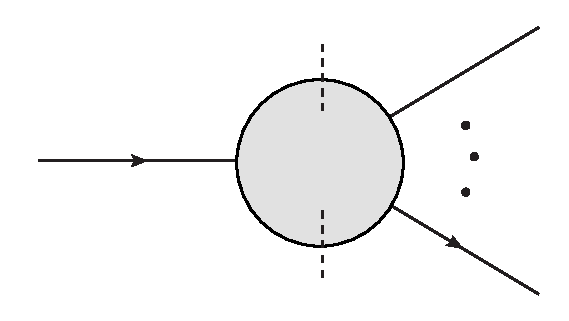
\includegraphics[height=12ex]{./figures/dc_div_left.eps}}} =
        \vcenter{\hbox{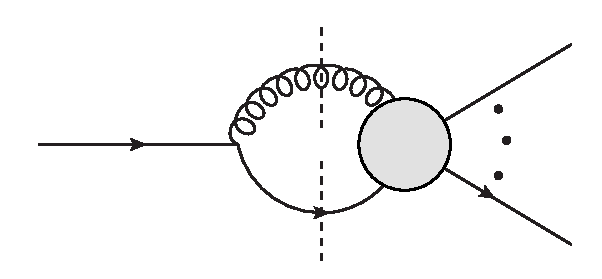
\includegraphics[height=12ex]{./figures/dc_div_r.eps}}}~+~
        \vcenter{\hbox{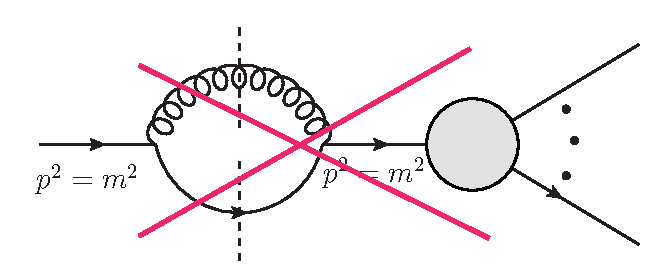
\includegraphics[height=12ex]{./figures/dc_div2_cross.eps}}}
      \]
      \caption{
        A double cut with the single on-shell massive quark in the corner (on the left), containing
        a divergent contribution associated to the mass and wave-function renormalization (the second term on the right),
        which has to be manually removed.
      }
      \label{fig:wbb:singdoublecut}
    \end{figure}
    Following the approach of \cite{Ellis:2008ir} we have implemented the removal of this contributions in our off-shell recursion.

  \item The topology in \cref{fig:dc_div2}, in addition to containing a divergent contribution mentioned above,
    has another special feature: the transverse complement of its single light-like external momentum contains this momentum.
    We discussed this in \cref{sec:ms_examples}.
    \begin{figure}[h]
      \centering
      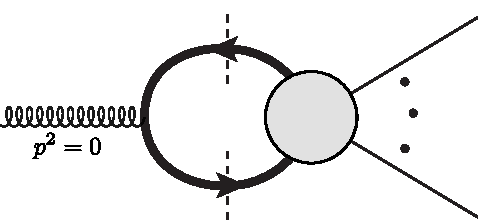
\includegraphics[width=0.3\textwidth]{dc_div2}
      \caption{A special one-loop topology with a massless on-shell leg in the corner and massive cut propagators.}
      \label{fig:dc_div2}
    \end{figure}
    This has two consequences. First, there are more coefficients with master integrals, and we evaluate the corresponding integrals explicitly.
    Second, as opposed to other one-loop topologies, the ansatz for the integrand of this topology is \emph{not} invariant under loop momentum shifts.
    This slightly complicates the construction of hierarchies, since it implies that the tadpoles below have to be carefully aligned.
    Interestingly, this is a generic feature beyond one loop, i.e.\ the ansätze for integrands of \emph{all} topologies are not invariant under loop momenta shifts.
\end{enumerate}


\paragraph{Integrals with internal masses.} Finally,
we have implemented all one-loop master integrals with real internal masses to $\order{\epsilon^0} $, based
on the results from \cite{Carrazza:2016gav,vanHameren:2010cp}. This allows us to incorporate
them in our automated numerical precision tracking and rescue system.

%%%%%%%%%%%%%%%%%%%%%%%%%%%%%%%%%%%%%%%%%%%%

\section{Setup}
\label{sec:wbb:setup}

\subsection{Channels}
\label{sec:calcsetup}

We compute NLO QCD corrections for the production of \Wbb~in association with $n$ light jets ($n =
0,1,2,3$) at the LHC $\sqrt{s} = 13$ TeV. 
We include the leptonic decays of the off-shell vector bosons at the level of amplitudes.
The parton-level cross-sections are obtained from the following channels:
\begin{subequations}
  \begin{align}
    n=0:&\qquad 0\rightarrow Wb{\bar b}q{\bar q}'\ ,\\
    n=1:&\qquad 0\rightarrow Wb{\bar b}q{\bar q}'g\ ,\\
    n=2:&\qquad 0\rightarrow Wb{\bar b}q{\bar q}'gg\ ,\quad  0\rightarrow Wb{\bar b}q{\bar q}'Q{\bar Q}\ ,\\
    n=3:&\qquad 0\rightarrow Wb{\bar b}q{\bar q}'ggg\ ,\quad  0\rightarrow Wb{\bar b}q{\bar q}'Q{\bar Q}g\ ,
  \end{align}
\end{subequations}
which we wrote in a crossing-symmetric form. 
Here the light quarks are denoted with $q$ and $Q$, and the $b$ quarks are considered massive.
The contributions from closed $b$ and $t$ loops are included. \footnote{
  Although the contribution of the latter is negligible.
}
We demonstrate some representative Feynman diagrams contributing to the channels of \Wbbjjj{} in \cref{fig:FDsWbb3j}.

We consider fixed order predictions at parton-level and discard parton-shower
effects. We will require exactly two tagged infrared-safe $b$ jets \cite{Banfi:2006hf}
in all observables we examine.

\begin{figure}[h]
  \centering
  \subfloat[][$qg\rightarrow q^\prime g g W^{\pm}b\bar{b}$]{ 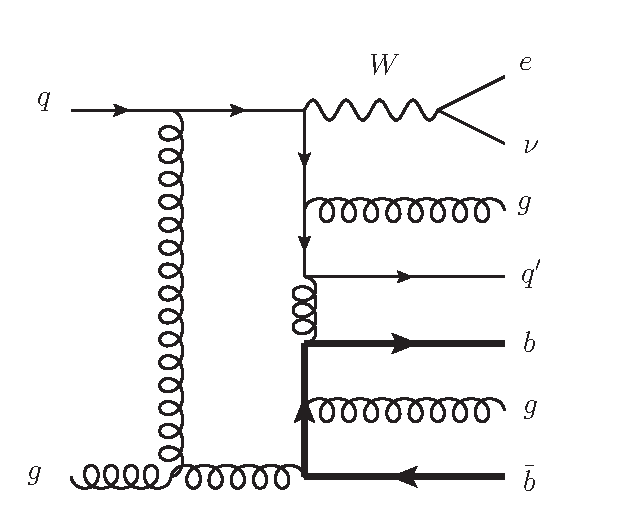
\includegraphics[width=0.28\textwidth]{figures/Wbb2q3g}}
  \qquad
  \subfloat[][$qg\rightarrow q^\prime g g W^{\pm}b\bar{b}$]{\label{subfloat:nf} 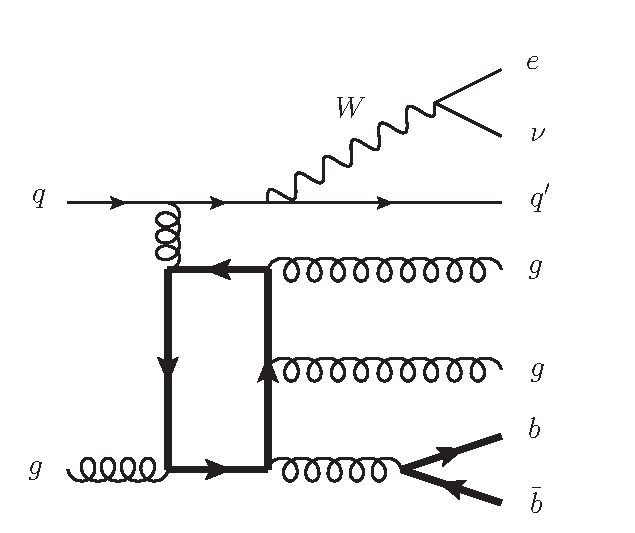
\includegraphics[width=0.28\textwidth]{figures/Wbb2q3g_nf}}
  \quad
  \subfloat[][$q{\bar Q}\rightarrow q^\prime \bar{Q} g W^{\pm}b\bar{b}$]{ 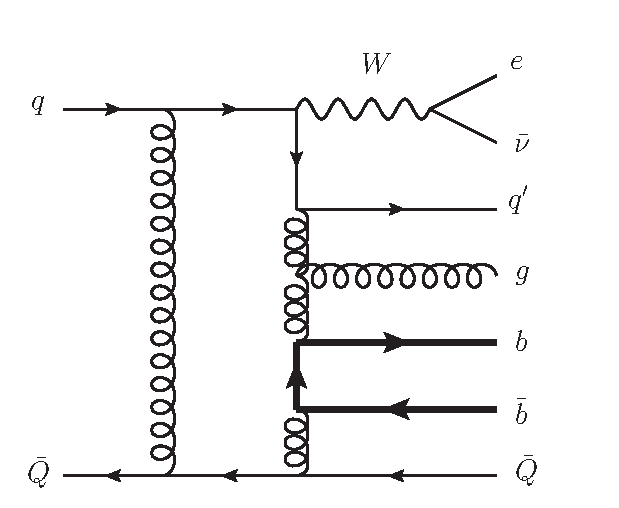
\includegraphics[width=0.28\textwidth]{figures/Wbb4q1g}}
  \caption{Representative one-loop diagrams contributing
    to \mbox{$pp\rightarrow$ \Wbbnj[3]{}} production. Massive quark
    lines are printed thick and the diagram \protect\subref{subfloat:nf} displays a contribution from closed loops of top and bottom quarks.}
  \label{fig:FDsWbb3j}
\end{figure}



\subsection{Renormalization}

We regularize UV and IR divergences in the FDH scheme in the computation of virtual matrix elements,
and use the known transition rules to convert our results to the HV scheme.

\todo{fix error in renormalization}

We give all counter-terms required for the renormalization in the FDH scheme, as well as additional finite shifts in \cref{tab:renorm}.
For the mass and wave-function renormalization we use the on-shell scheme,
and for the $\overline{\text{MS}}$ scheme for the QCD coupling.
\begin{table}[h]
  \begin{tabular}{lcll}
    \textbf{Renormalization} & \textbf{Scheme} & \textbf{Counterterm} \\
    \toprule
    Heavy quark wave function   & on-shell & $\displaystyle \delta_{2,i} ~=~ \frac{N_c^2-1}{2N_c} \left( \frac{3}{\epsilon} + 5 + 3 \ln{\frac{\mu^2}{m_i^2}} \right)$\\
    Light quark wave function   & on-shell & 0\qquad(UV+IR cancellation) \\
    Quark mass            & on-shell & $\displaystyle \delta_{m_i} ~=~ \delta_{2,i}\quad\text{}$\\
    Gluon wave function   & on-shell & $\displaystyle \delta_3 ~=~ \frac{3}{\epsilon} + \sum_i \frac{1}{3}\ln{\frac{\mu^2}{m_i^2}}$\\
    QCD coupling & $\overline{MS}$ & $\displaystyle \delta_{\alps} ~=~ \frac{1}{\epsilon} \left( \frac{11}{3}N_c - \frac{2}{3}(N_f+N_h) \right) - \frac{N_c}{3}$\\
    \midrule
    Decoupling shift & --- & $\displaystyle     \Delta_i ~=~  -\frac{2}{3}\ln{\frac{\mu^2}{m_i^2}} $\\
    \bottomrule
  \end{tabular}
  \caption{The renormalization counter-terms. Here $\mu$ is the renormalization
    scale, $m_{i}$ are the masses for heavy quarks, $N_f$ is the number of light flavors,
    $N_h$ the number of heavy flavors, and $N_c$ the number of colors.
  }
  \label{tab:renorm}
\end{table}
We set $N_f=4$, and $N_h=2$, as we work in the 4FNS, and 
add the decoupling shifts for top and bottom quarks to correctly reproduce the corresponding decoupling limits.
Except for the mass renormalization, which we perform via an explicit computation,
the whole renormalization is proportional to the tree amplitude, 
and the renormalized amplitude $\mathcal{A}^{(ren)}$ is
obtained as
\begin{equation}
  \mathcal{A}^{(ren)} =
  \mathcal{A}^{(bare)}_{m_R} - 4\pi \alpha_s c_\Gamma 
  \left( \sum_i N_{Q_i} \frac{\delta_{2,i}}{2} + N_{g}\delta_3 + \frac{N_{\alps}}{2}\left(\delta_{\alps} + \sum_{i\in N_h}\Delta_i\right) \right)  \mathcal{A}^{(born)},
  \label{renfull}
\end{equation}
where $\mathcal{A}^{(bare)}_{m_R}$ is the amplitude with renormalized masses,
$\displaystyle c_\Gamma={(4\pi)^{-(2-\epsilon)}{\Gamma(1+\epsilon)\Gamma^2(1-\epsilon)}/\Gamma(1-2\epsilon)}$,
$N_g$ and $N_{Q_i}$ are the numbers of external gluons and heavy quarks of flavor $i$ correspondingly,
and $N_{\alps}$ is the power of $\alps$ of the tree amplitude.
We shift \cite{Signer:2008va} the amplitude by
\begin{equation}
  \mathcal{A}^{(ren)}_{HV} - \mathcal{A}^{(ren)}_{FDH} = -4\pi \alpha_s c_\Gamma\left(N_{g}~\frac{N_c}{6} + \frac{N_q}{4}\left(N_c -\frac{1}{N_c}\right)\right)\mathcal{A}^{(born)},
  \label{schemeshift}
\end{equation}
to convert it to the HV scheme.



\subsection{Validation}

The upgrade to the new version of \BlackHat{} involved significant new developments,
as well as replacing a considerable number of old components.
We have extensively validated the new version with the following checks:
\begin{enumerate}
  \item We have reproduced all amplitudes available in \BlackHat{} before the upgrade.
  \item We perform a number of automated internal consistency checks:
    \begin{itemize}
      \item We extend the ansatz for the integrands on the right-hand side of \cref{eq:cut_equations} with the terms which are guaranteed to be zero, for example, by the power-counting constraints.
        We then solve the equations for the coefficients, and check if the coefficients of these term vanish.
      \item We check the known pole structure \cite{Catani:2000ef} of each primitive amplitude.
    \end{itemize}
  \item We have checked the IR poles of squared matrix elements against the integrated subtraction terms,
    as implemented in the \SHERPA{} library.
  \item We have reproduced the helicity amplitudes from \cite{Ellis:2008ir}.
  \item We have performed a systematic comparison of squared matrix elements 
    of all subprocesses of $pp\rightarrow t\bar t+(\leq 2)-$jet, $pp\rightarrow b\bar b+(\leq 2)-$, and
$Wb\bar b+(\leq3)-$ processes against publicly available generators 
\textsc{Recola}~\cite{Actis:2016mpe} and \textsc{OpenLoops}~\cite{Cascioli:2011va} 
(both powered by the \textsc{Collier} library~\cite{Denner:2016kdg}).
\end{enumerate}

\subsection{Numerical Stability}
%
In this section, we explore the numerical stability of the new version of \BlackHat{}.
We compare the normal matrix elements $d\sigma_V^\mathrm{prod}$ with the ones obtained from quadruple-precision evaluations $d\sigma_V^\mathrm{HP}$.\footnote{
  We use the \cite{QD} library for high-precision arithmetics
}

\begin{figure}[h]
  \centering
  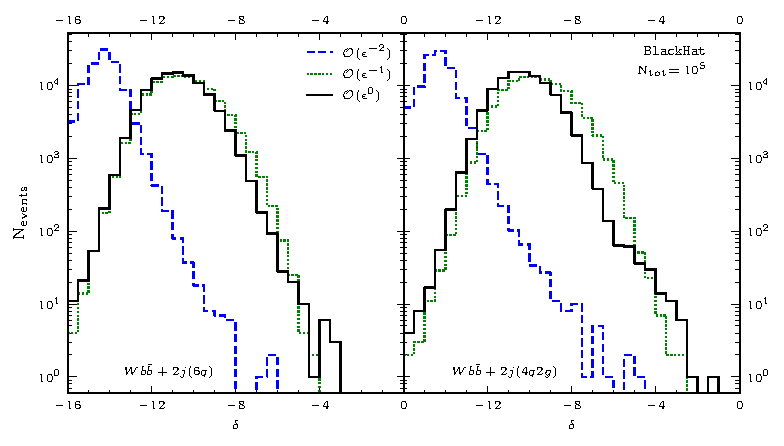
\includegraphics[scale=1.1]{plots/numstab2j}
  \caption{
    The logarithmic relative error of the full-color matrix elements
    for two types of subprocesses contributing to the \Wbbjj~production calculation. On the
    left we show results for the
    six-quark and on the right for four-quark matrix elements, respectively.
    The dashed (blue) line represents the precision of the double pole, the dotted
    (green) line represents the single pole and the
  solid (black) line the precision of the finite piece of the calculation.}
  \label{fig:stabilityWbb2j}
\end{figure}
\begin{figure}[h]
  \centering
  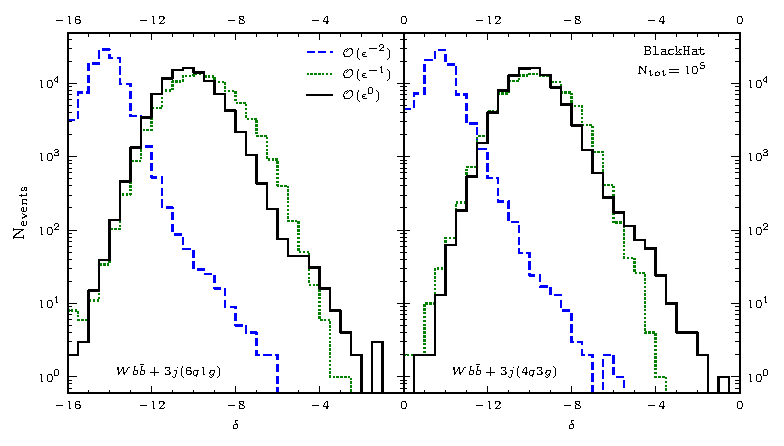
\includegraphics[scale=1.1]{plots/numstab3j}
  \caption{As in \cref{fig:stabilityWbb2j} but for \Wbbjjj{} production,
  considering only the leading-color contributions to the one-loop matrix elements.
  On the left we show results associated to the six-quark and on the right the ones associated to
four-quark matrix elements.}
\label{fig:stabilityWbb3j}
\end{figure}


We study the most complex sub-processes
by generating the histograms (see \cref{fig:stabilityWbb2j,fig:stabilityWbb3j}) of the logarithmic relative error $\delta$,
\begin{equation}
  \delta = \log_{10}\left(\frac{\left|d\sigma^{\text{prod}}_V - d\sigma^{\text{HP}}_V\right|}{\left|d\sigma^{\text{HP}}_V\right|}\right)\ .
  \label{reldiff}
\end{equation}
We sample $10^5$ phase-space points from the same distribution that we used in our phenomenological studies.
Overall we see, that our program is numerically stable,
with only a few points with precision worse then $10^{-3}$,
which have no effect on the observables.

One of the advantages of unitarity methods is that they allow a fine-grained control of the evaluation process.
We convert all the internal consistency tests listed in the previous section into
the precision-monitoring system.  
It identifies when the computation becomes unstable, and reevaluates
only the small part with higher precision whenever required.



\section{Monte Carlo Integration}
\label{sec:wbb:mc_integration}



We employ \SHERPA{}\cite{Sherpa} for managing the Monte-Carlo integration,
subprocess generation and phase-space mappings.
And we interface it to our library for virtual matrix-element generation.
We split the virtual matrix elements into leading and subleading color contributions
to optimize the integration. The latter are more expensive to compute, but contribute less to the observables,
so they can be samples less frequently \cite{BH:W3jDistributions,Ita:2011ar}.
We employ massive dipoles \cite{Catani2002} for IR subtraction as implemented in \COMIX{}~\cite{Comix}.
%

We perform a fixed-order parton-level computation. Non-perturbative effects, such as hadronization, as well as parton showers are considered in our study.
All results that we provide are fixed-order parton-level predictions and we include neither parton-shower effects nor hadronization corrections or other
non-perturbative effects.

\subsection{Input Parameters: Partons Distributions, Couplings and Masses}
\label{sec:base_setup}
We use PDFs from {\texttt CT14}~\cite{CT14},
with LO ({\texttt CT14llo\_NF4}) and NLO ({\texttt CT14nlo\_NF4}) PDF sets, as
implemented in the LHAPDF library~\cite{LHAPDF}. 
The strong coupling is taken to by $\alps(M_Z)=0.125$ at LO and
$\alps(M_Z)=0.1128$ at NLO. 
The bottom-quark mass is $m_b=4.75$ GeV.

The electroweak parameters are evaluated in the LO $G_\mu$ scheme \cite{Denner2000c}. The fixed and computed
parameters as given in \cref{tab:ewinput}. The $\alpf(M_Z)$,
$\sin^2(\theta_W)$ and $g_W^2$ are computed with
\begin{align}\label{eq:ewlorel}
\sin^2(\theta_W) &= \left(1-\frac{M_W^2}{M_Z^2}\right)\ , & \alpf(M_Z)&=\frac{\sqrt{2}}{\pi}G_F M_W^2
  \sin^2(\theta_W)\ ,\notag\\
g_W^2&=\frac{4\pi\alpf(M_Z) }{\sin^2(\theta_W)}\ .
\end{align}

\begin{table}[]
  \centering
  \begin{tabular}{p{3.5cm}p{5cm}}
    \toprule
    Parameter & Value  \\
    \midrule
    $G_F$ & $1.1663787 \times 10^{-5}$ GeV$^{-2}$ \\
    $M_W^{\text{OS}}$& $80.385$ GeV \\
    $M_Z^{\text{OS}}$& $91.1876$ GeV \\
    $\Gamma_W$& $2.085$ GeV \\
    $\alpf(M_Z)$ & $1/132.23$ (calculated)\\
    $\sin^2(\theta_W)$ & $0.22290$ (calculated)\\
    $g_W^2$ & $0.42635$ (calculated)\\
    \bottomrule
  \end{tabular}
  \caption{Electroweak parameters used in our study, which are chosen in accordance with 2016 PDG values~\cite{Patrignani:2016xqp}.}
  \label{tab:ewinput}
\end{table}

The CKM matrix is approximated by a unit matrix. 
The leads to difference of  the order of at most 1\%,
as determined from the LO analysis.

We find that the contribution of the closed top quarks has a order $1\%$ effect on
the cross-sections. This is according to expectations ~\cite{BH:W4j,BH:Z4j,Campbell:2016tcu}. 

\subsection{Kinematics, Observables and Exclusive Sums}
\label{sec:kin}
In this section, we provide the definition for observables we employ in our study.
The pseudorapidity $\eta$ and the
angular separation between two partons, leptons, or jets $\Delta R$ are defined as
\begin{align}
  \eta &= -\ln\left(\tan\frac{\theta}{2}\right),&  \Delta R &= \sqrt{(\Delta \phi)^2+(\Delta \eta)^2}.
\end{align}
Here $\Delta\phi$ is the difference in the azimuthal angle in the transverse plane,
$\theta$ is the polar angle with respect to the beam axis, and
$\Delta\eta$ the difference in $\eta$. 
The transverse energy of $W$, $E_T^W$, and the total partonic transverse energy $\HTpartonicp$ are defined as
\begin{align}\label{eq:htpart}
  E_T^W&=\sqrt{M_W^2+\left(p_T^W \right)^2},& \HTpartonicp&=\sum_j p_{\textrm T}^j+E_{\textrm T}^W, \qquad p_T=\sqrt{p_x^2+p_y^2}
\end{align}
with the sum over all final state partons $j$.
The jet invariant masses are defined by
\begin{align}
  M_{ij}^2 = \left(p_i^{\text{jet}}+p_j^{\text{jet}}\right)^2,
\end{align}
and we label  jets in order of decreasing transverse momentum $p_T$. 
The transverse mass of $W$ is
\begin{align}
  M_T^W=\sqrt{2E_T^eE_T^\nu(1-\cos(\Delta\phi_{e\nu}))}\ .
\end{align}

We now explain how do we build the exclusive-sum observables from multi-jet samples.
We choose the cut $p_{T}^{\text{excl}}$, with respect to which we take an exclusive cross-section $\sigma^{\text{exc}}_n$
for each jet multiplicity $n$, except the one with maximal  $n$, for which we take the inclusive result,
\begin{align}\label{eq:excsums}
  \sigma^{\text{NLO+}}_0 &= \sigma^{\text{exc}}_0 + \sigma^{\text{inc}}_1\ , &
\sigma^{\text{NLO++}}_0 &= \sigma^{\text{exc}}_0 +\sigma^{\text{exc}}_1+
\sigma^{\text{inc}}_2\ .
\end{align}
The expectation is that replacing the, effectively leading order contributions, from the real radiation with the full NLO
corrections mitigates the problem of large $K$ factors, and at the time, the sensitivity to $p_{T}^{\text{excl}}$ is not as high 
as in the case of the exclusive computation.

\section{Phenomenology}
\label{sec:wbb:pheno}
In this section we present NLO QCD results for \Wbbn~production in
$pp$ collisions at $\sqrt{s}=13$ TeV, the experimental configuration
of the LHC Run-II. We present results for a set of distributions and
apply the following cuts
\begin{align}
  p_T^{\text{jet}}&>25\text{ GeV},& |\eta^{\text{jet}}|&<2.4\ ,\notag\\
  p_T^{e}&>25\text{ GeV},& |\eta^{e}|&<2.5\ ,\notag\\
  p_T^{\nu}&>20\text{ GeV},& M_T^W &> 20\text{ GeV}\ .
  \label{eq:Cuts}
\end{align}
The cuts are applied to both light  and
$b$ jets. The renormalization and factorization scales are chosen to be equal and set on an
event-by-event basis by $\mu=\HTpartonicp/2$, according to
\cref{eq:htpart}. We define our jets by employing the
anti-$k_T$ jet algorithm~\cite{antikT} with $R=0.4$, as implemented in the
\texttt{FastJet} package~\cite{Cacciari:2011ma}.

\subsection{Total Cross Section and Scale Dependence}
\label{totalxsw}
In \cref{tab_Wpj_total_xs}, we present total partonic cross sections,
employing the kinematical cuts of \cref{eq:Cuts}, for inclusive production of
both $W^-$ and $W^+$ accompanied by two $b$ jets and zero to three
light jets. The numerical integration uncertainty is given in parenthesis and
the scale dependence is quoted in superscripts and subscripts. We also show
the ratio of NLO over LO results, so called $K$-factors, in separate columns.

We employ the standard dynamical choice of factorization and renormalization scales $\mu_R=\mu_F=\mu_0=\HTpartonicp/2$ (see \cref{eq:htpart}).
We estimate the error from the missing orders of the perturbation series expansion in the coupling constants with the standard technique of
the scale variations around the central scale $\mu_0$. 



%%%%%%%%%%%%%%%%%%%%%%%%%%%%%%%%%%%%%%%%%%%%%% 
\begin{table}[ht]
  \begin{center}
    \begin{adjustbox}{width=1\linewidth}
      \begin{tabular}{ccccccc}
        \toprule
        jets  & \Wbbm~LO & \Wbbm~NLO & $K$-factor & \Wbbp~LO & \Wbbp~NLO & $K$-factor\\
        \midrule
        0  & $0.33278(12)^{+0.0619}_{-0.0490}$ & $0.67719(60)^{+0.1288}_{-0.1000}$  & $2.03$ & $0.48573(19)^{+0.0925}_{-0.0727}$ & $0.97175(85)^{+0.1877}_{-0.1411}$  & $2.00$\\
        1  & $0.36153(13)^{+0.1408}_{-0.0945}$ & $0.50484(63)^{+0.0851}_{-0.0800}$  & $1.40$ & $0.52095(23)^{+0.2034}_{-0.1362}$ & $0.72740(99)^{+0.1277}_{-0.1167}$  & $1.40$\\
        2 & $0.18501(44)^{+0.1053}_{-0.0626}$ & $0.22604(87)^{+0.0407}_{-0.0400}$  & $1.22$ & $0.27663(68)^{+0.1569}_{-0.0934}$ & $0.3340(17)^{+0.0599}_{-0.0647}$  & $1.21$\\
        3  & $0.07204(25)^{+0.0540}_{-0.0289}$ & $0.08288(89)^{+0.0189}_{-0.0200}$  & $1.15$ & $0.11493(59)^{+0.0855}_{-0.0459}$ & $0.1286(17)^{+0.0280}_{-0.0307}$  & $1.12$\\
        \bottomrule
      \end{tabular}
    \end{adjustbox}
     %%%%%%%%%%% TABLE xs  %%%%%%%%%%%%%%%%%%%%%%%%%%
  \end{center}
  \caption{LO and NLO QCD results for inclusive \Wbbpm+$0,1,2,3$-jet cross
    sections (in $pb$). Results with dynamical scale $\HTpartonicp/2$ are shown
    together with their respective $K$-factors.  The setup employed is specified in
    section~\ref{sec:kin}, and kinematical cuts in \cref{eq:Cuts}. Scale
    dependence is shown in superscripts and subscripts. The number in parenthesis next to
    the central value gives the corresponding statistical integration
    error.\label{tab_Wpj_total_xs} }
  \end{table}


%%%%%%%%%%% TABLE ratios  %%%%%%%%%%%%%%%%%%%%%%%%%%
  \begin{table}[ht]
    \small
    \begin{center}
      \begin{adjustbox}{width=1\linewidth}
        \begin{tabular}{ccccccc}
          \toprule
          \multicolumn{1}{c}{ } & \multicolumn{2}{c}{\Wbbp~$n$/\Wbbm~$n$} &
          \multicolumn{2}{c}{\Wbbm~$n/(n-1)$}  &
          \multicolumn{2}{c}{\Wbbp~$n/(n-1)$} \\
          $\qquad n\qquad$ & LO & NLO & LO & NLO  & LO & NLO  \\
          \midrule
          0 &  $1.45962(78)$ & $1.4350(18)$ & --- &  --- & ---  & --- \\
          1&  $1.44098(83)$ & $1.4409(27)$ & $1.08640(55)$ &$ 0.7455(17)$ &$ 1.07253(64)$ & $ 0.7485(12)$ \\
          2&  $1.4952(51)$ & $1.4776(95)$ & $0.5117(12)$ &$ 0.4478(21)$ &$ 0.5310(13)$ & $ 0.4592(24)$ \\
          3&  $1.5952(99)$ & $1.551(27)$ & $0.3894(16)$ &$ 0.3667(44)$ &$ 0.4155(24)$ & $ 0.3850(54)$ \\
          \bottomrule
        \end{tabular}
      \end{adjustbox}
     %%%%%%%%%%% TABLE xs  %%%%%%%%%%%%%%%%%%%%%%%%%%
    \end{center}
    \caption{LO and NLO QCD cross section ratios. The second and third columns
      give charge ratios for both LO and NLO cross sections as a function of the number of
      associated light jets $n$. The last four columns give jet
      production ratios for both \Wbbm~as well as \Wbbp~in association with $n$ light
      jets. These ratios are taken for the cross section of a given
      process to that with one less jet. The number in parenthesis gives the corresponding statistical integration error.\label{tab_xs_ratios} }
    \end{table}
%%%%%%%%%%% TABLE ratios  %%%%%%%%%%%%%%%%%%%%%%%%%%




LO cross sections display a large scale sensitivity, reaching up to 60\% for
\Wbbjjj{} production. We note that the scale dependence of the LO cross section
for \Wbb{} is around $20\%$ while the NLO QCD corrections increase the
total cross section by a factor of 2. This clearly highlights that scale
dependence is in general not representative of the associated theoretical
uncertainties. In this case, the large quantum corrections can be understood as a
result of the opening of gluon-initiated
channels~\cite{Ellis:1998fv,FebresCordero:2006sj,Cordero:2009kv}. Also for \Wbbj{} a gluon-gluon initiated channel is opened
up, but with milder impact, and for the larger multiplicity processes all
subprocesses are present at LO. Hence, quantum corrections are milder
for these processes. Furthermore, kinematical
constraints at LO are only present for \Wbb{} production, as we will discuss for example for the $p_T^{b\bar b}$ and
$p_T^W$ observables in \cref{sec:hw}. As a consequence, we expect quantum corrections for
processes with even more light jets to be under relatively good pertubative control.


In \cref{tab_xs_ratios} we show first, in columns 2 and 3, $W^+/W^-$ charge
ratios as a function of the number of jets. These ratios show a large stability
with respect to the quantum corrections, which have been explored in similar
processes as a way to make precise determinations of ratios of $u/d$ PDFs (see
for example ref.~\cite{Kom:2010mv}). They also show some stability as a function
of the number of jets, with a slight monotonic increase given the larger mean
values of Bjorken $x$ sampled as a consequence of the larger invariant mass necessary to
produce the corresponding final states.

Finally we also explore in \cref{tab_xs_ratios} the jet ratios in $W^\pm
b\bar b$ production in association with light jets. Similarly to studies of these ratios in $W+n$-jet (light jet)
production~\cite{BH:Wratios}, we observe that the results for $n=1$ are special
given the large NLO corrections for \Wbb{} production. The opening of an
initial-state channel makes the
\Wbbj{}$/$\Wbb{} ratio clearly sensible to quantum corrections. In the light jet
study~\cite{BH:Wratios} this was the case for the ratio ($W+2$-jet$)/$($W+1-$jet),
and a full study of jet-ratio universality needed the completion of the NLO QCD
correction to $W+5$-jet production~\cite{BH:W5j}. Similarly, in \Wbb{} inclusive
production, it might be interesting to explore the NLO QCD corrections to
$W+b\bar b+4$-jet production in the future.

In \cref{fig_Wjets_sdep} we study the dependence of total cross sections in
\Wbbm{} and \Wbbp{} production in association with up to 3 light jets on the
renormalization and factorization scale. We employ the central dynamical scale
$\mu_0=\mu_\mathrm{R}=\mu_\mathrm{F}=\HTpartonicp/2$. The scale variations
observed for $W^+$ and for $W^-$ are very similar. The LO cross sections have a monotonically increasing
scale dependence, for $n\geq 1$.  As we observed in the previous subsection, the
scale dependence of \Wbb{} production is special.


%scale dependence for Wm
%%%%%%%%%%%%% FIGURE %%%%%%%%%%%%%%%%%%
\begin{figure}[ht]
\begin{center}
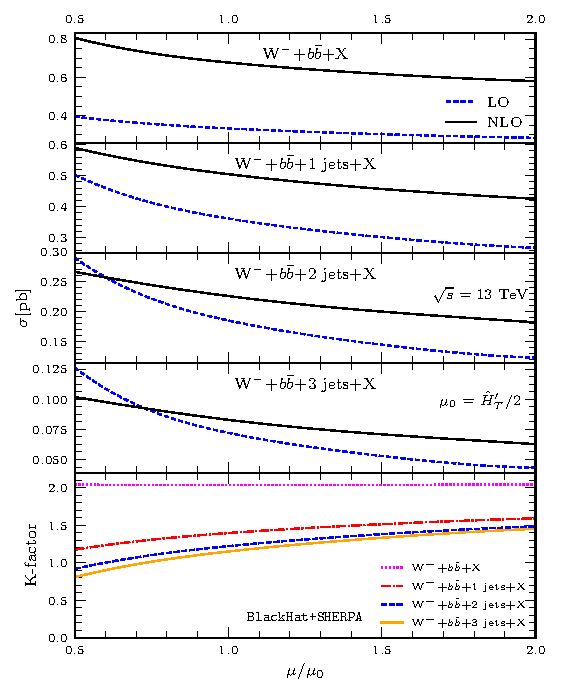
\includegraphics[clip,scale=0.71]{plots/scale_dependence_Wmbb}
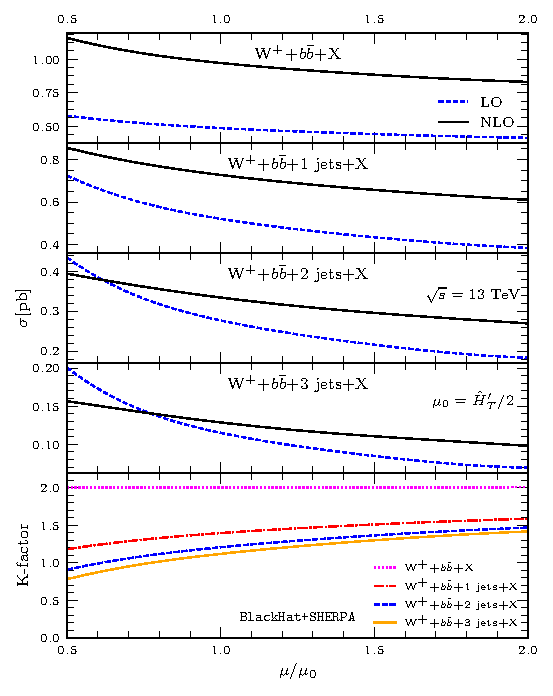
\includegraphics[clip,scale=0.71]{plots/scale_dependence_Wpbb}
\end{center}
\caption{The renormalization- and factorization-scale dependence of total cross
  sections for \Wbbm$+0,1,2,3$-jet$+X$ production in the left and
\Wbbp$+0,1,2,3$-jet$+X$ production to the right,
 with $\mu_0=\mu_\mathrm{r}=\mu_\mathrm{f}=\HTpartonicp/2$. 
The upper four panels show the dependence of LO (dashed blue line) and
  NLO (solid black line) predictions. The lower panel shows
  the K-factor (ratio of NLO/LO).}
\label{fig_Wjets_sdep}
\end{figure}
%%%%%%%%%%%%%%%%%%%%%%%%%%%%%%%%%%%%%%%

We choose the dynamical scale $\HTpartonicp/2$ which on average increases monotonically with multiplicity. For vector boson production in association with massless jets this scale choice
has been observed to produce stable NLO results over a wide range of kinematical
configurations relevant to the LHC and future
colliders~\cite{BH:W3jPRL,BH:W4j,BH:W5j,Mangano:2016jyj}. For the LHC in
particular, it has been observed that for massless jet production the scale
$\HTpartonicp/2$ typically produced NLO cross sections lying on the locus of the
scale-dependence curves. Here we observe that for \Wbbn{} production, the
NLO cross section at the central scale appears consistently on the right of the
scale-dependence plateau. We can assert, in particular considering the
similarities of the massive and massless results studied in
section~\ref{sec:bmass}, that this difference has little to do with the presence
of a massive jet, and it is actually due to the dominant type of subprocess. For
light-jet production those are the ones with a single quark line, while in
the case of \Wbbn{} production the dominant subprocess are those with
two quark lines (those are the subprocesses with most gluons allowed).

Another interesting difference between $W$ production in association with light
jets and \Wbb{} production with multiple light jets, is that for the
former the leading-color approximation for one-loop matrix elements gave a very good
approximation for physical observables (at the level of 1 to
3\%). Contrary to that, \Wbb{} production with light jets is largely dominated by virtual
contributions in our setup, and so the leading-color approximation is at the
order of 10\% for physical observables. That is why all of our results in this
article include full-color information, and we only
exploit the decomposition in a color expansion for efficiency of the
computation. We again attribute this difference to the unlike dominant
subprocesses.


\subsection{Differential distributions}
\label{diffxsw}

In this section, we describe NLO results for several differential
distributions and thereby analyze the impact
that quantum corrections have on fixed-order predictions over phase
space. We generally show results only for one of the $W^\pm$ charges, as the
structure of the corrections are similar between them. 

%pt leading bjet
%%%%%%%%%%%%% FIGURE %%%%%%%%%%%%%%%%%%
\begin{figure}[ht]
  \centering
  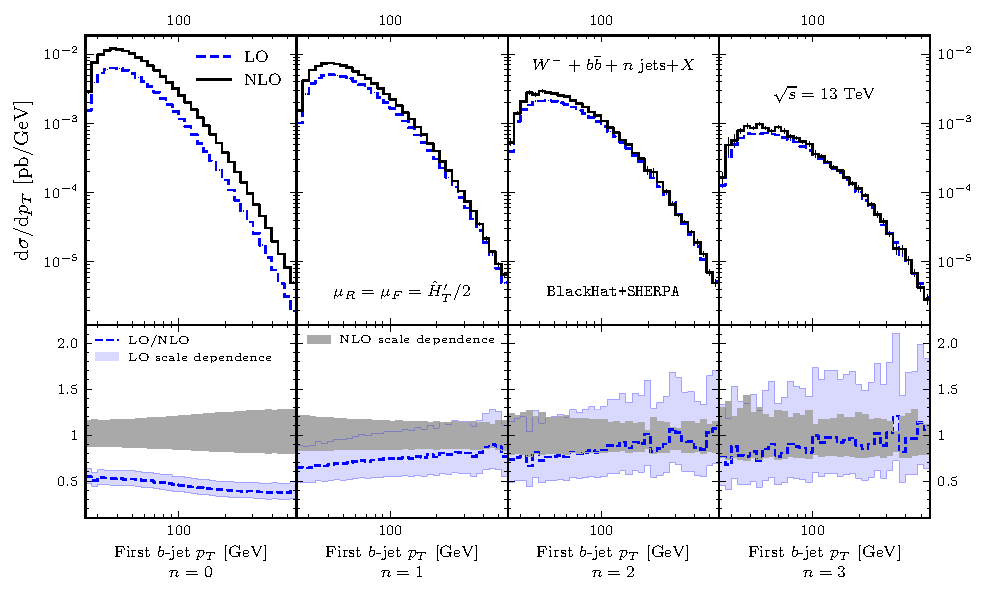
\includegraphics[clip,scale=1]{plots/ptleading}
  \caption{The $\pT$ distributions of the leading $b$ jet (ordered by $p_T$) in inclusive \Wbbm$+n$-jet
    production at the LHC with $\sqrt{s}=13$~TeV. The light-jet multiplicity 
    increases from $n=0$ to $n=3$ from left to right. In the upper panels the
    dashed (blue) lines show the LO results and the solid (black) lines the NLO
    results. Vertical thin lines show the statistical error from the numerical
    integration. In the bottom panels we show the scale-dependence bands
  normalized to the NLO result, in blue for LO and dark gray for NLO.}
  \label{fig_Wmnjpt}
\end{figure}
%%%%%%%%%%%%%%%%%%%%%%%%%%%%%%%%%%%%%%%

%pt subleading bjet
%%%%%%%%%%%%% FIGURE %%%%%%%%%%%%%%%%%%
\begin{figure}[ht]
  \centering
  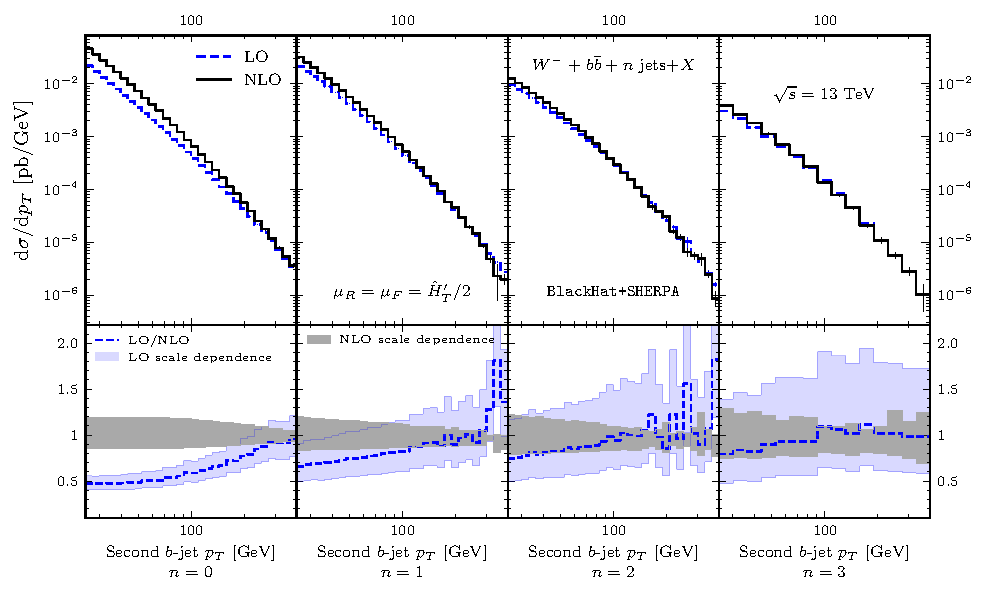
\includegraphics[clip,scale=1]{plots/ptsubleading}
  \caption{The $\pT$ distributions of the subleading $b$ jet (ordered by $p_T$) in inclusive \Wbbm$+n$-jet
    production at the LHC with $\sqrt{s}=13$~TeV. Format as in \cref{fig_Wmnjpt}.}
    \label{fig_Wmnjpt2}
  \end{figure}
%%%%%%%%%%%%%%%%%%%%%%%%%%%%%%%%%%%%%%%

In \cref{fig_Wmnjpt,fig_Wmnjpt2} we show the jet-$p_T$ spectra of the leading
and subleading $b$ jets (ordered by $p_T$) respectively, for inclusive
\Wbbm{} production in association with $n=0,1,2,3$ jets. The upper panel
of the
figures show the LO and NLO distributions in dashed (blue) and solid (black)
lines respectively, while the bottom panels show the scale-dependence bands
normalized to the central NLO result (LO in blue and NLO in gray). Numerical
integration errors for each bin are shown as thin vertical lines (when visible).
All distributions will be shown in a similar manner.

The NLO corrections show quite some structure beyond the $K$-factors studied at
the level of the total cross sections in the previous subsection. We
observe shape differences in most of the $p_T$ distributions of the $b$ jets, in a way
that make the LO predictions usually harder (with the exception of the leading
$b$ jet $p_T$ in \Wbb{} production). Nevertheless, the LO/NLO shape difference
is clearly reduced for the process with highest multiplicity, \Wbbjjj{} production, a
feature that shows up persistently in the following observables.
We notice that the scale dependence of the NLO
results is reduced compared to the LO results (apart from \Wbb{}, as
discussed for total cross sections). In the high multiplicity samples, the NLO results
lie inside the LO bands. 

%Softest light-jet PT
%%%%%%%%%%%%% FIGURE %%%%%%%%%%%%%%%%%%
\begin{figure}[ht]
  \centering
  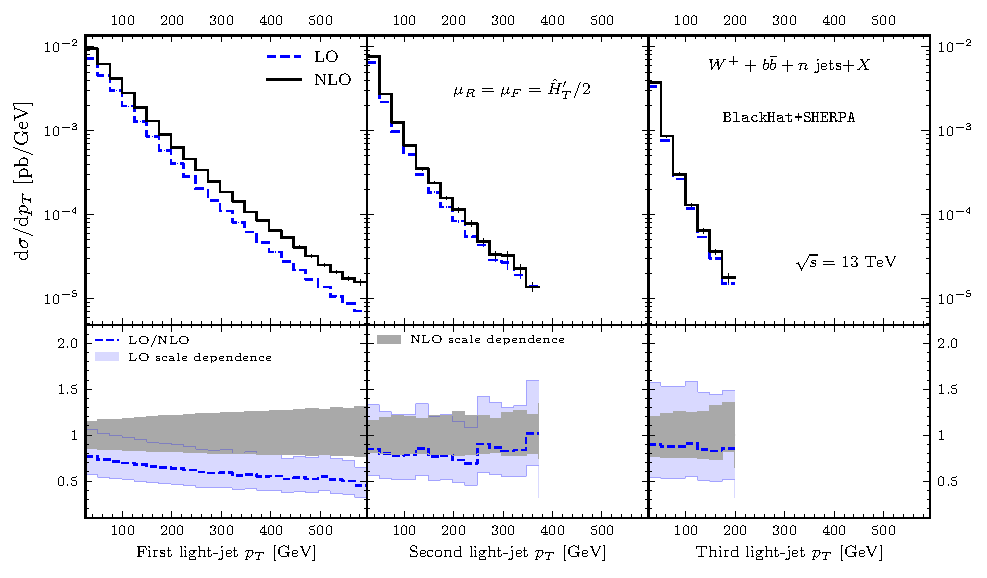
\includegraphics[clip,scale=1]{plots/softestpt}
  \caption{The $\pT$
    distributions of the softest light jet in inclusive \Wbbp$+n$-jet production.
    Format as in \cref{fig_Wmnjpt}.}
    \label{fig_Wmnjptlight}
  \end{figure}
%%%%%%%%%%%%%%%%%%%%%%%%%%%%%%%%%%%%%%%

In \cref{fig_Wmnjptlight} we show the $p_T$ distributions of the softest light jet in
inclusive \Wbbp{}$+1,2,3$-jet production. We observe a considerable reduction of the scale
sensitivity with the inclusion of the QCD corrections, with overlap of the LO
and NLO bands. It is important to note that for these distributions, which are
experimentally very relevant as they are quite sensitive to the jet-energy
scale, the quantum corrections are rather flat. The feature is similar to
what has been observed for softest jet $p_T$ distributions in $W+n$-light-jet
production, and which is associated to the choice of renormalization and
factorization scales $\HTpartonicp/2$ in the LO result. Notice that the NLO
results are rather insensitive to the choice of dynamical scale, as long as the
choice is naturally connected to the kinematic configurations of the processes
under study.

%HT jet / hadronic
%%%%%%%%%%%%% FIGURE %%%%%%%%%%%%%%%%%%
\begin{figure}[ht]
  \centering
  \includegraphics[clip,scale=1.0]{plots/htjets.pdf}
  \caption{Distribution in the total transverse jet energy
    $H_T^{jets}$ of light  and $b$ jets for inclusive \Wbbm$+n$-jet
    production at the LHC with $\sqrt{s}=13$~TeV. Format as in \cref{fig_Wmnjpt}.}
    \label{fig_Wmnjht}
  \end{figure}
%%%%%%%%%%%%%%%%%%%%%%%%%%%%%%%%%%%%%%%

An interesting observable for many scenarios of physics beyond the SM (BSM), as
well as for experimental studies at hadron colliders, is that of the total
hadronic activity in a detector. In \cref{fig_Wmnjht} we show the distribution in
this observable, including all hadronic activity from the light and $b$ jets in
\Wbbm$+0,1,2,3$-jet production. Large and phase-space dependent NLO
corrections appear for \Wbb{} as we would expect from previous discussions.
Interestingly, in \Wbbj{} production a remnant of these large effects appears
in this observable. The corrections are not as large as for the former, but still at
around 1~TeV for $H_T^{jets}$, we see a differential $K$-factor reaching two,
though the shape difference seems to end at about 400~GeV. The
large-multiplicity processes on the other hand show much less
structure, related to the kinematically unconstrained nature of their
LO configurations, which contain any $W$ soft enhancements starting at LO.

%dR first b-jet / charged lepton
%%%%%%%%%%%%% FIGURE %%%%%%%%%%%%%%%%%%
\begin{figure}[ht]
  \centering
  \includegraphics[clip,scale=1.0]{plots/drbl.pdf}
  \caption{Distribution in the $\Delta R_{bl^-}$ separation between the first
  $b$ jet (ordered in $p_T$) and the charged lepton for inclusive \Wbbm$+n$ jets
  production.  Format as in \cref{fig_Wmnjpt}.}
  \label{fig_Wmnjdrbl}
\end{figure}
%%%%%%%%%%%%%%%%%%%%%%%%%%%%%%%%%%%%%%%

Finally, to end this section, we show in \cref{fig_Wmnjdrbl} the distribution
on the $\Delta R$ separation between the first $b$ jet and charged lepton $l^-$. Most
of the angular variables that we have studied are similar to this one, which
shows little structure in the QCD corrections. We only find effects
when a certain kinematic constraint is imposed at LO and released by the corrections,
as it is the case on the left most plots of \cref{fig_Wmnjdrbl}. 
In the case of the $\Delta R_{bl^-}$ at LO in \Wbbm{} production, the parent $W$
and gluon that give rise to the leptons and $b$ jets are produced with $\Delta
\phi$ (the difference in azimuthal angle) equal to $\pi$. Also, the $\Delta \eta$
distribution peaks at around zero and decreases monotonically. The resulting $\Delta R_{bl^-}$ distribution thus has the feature of a sharply decaying
distribution at LO. All
those constrains are lifted by the real corrections and do not appear at all in
\Wbb$+1,2,3$-jet production.


\subsection{Finite $b$ Mass Effects}
\label{sec:bmass}
Mass effects in \Wbb{} have been studied since the early NLO QCD
calculations in ref.~\cite{FebresCordero:2006sj}. They are expected to be small when two
well-defined $b$ jets are considered, and ratios of $m_b^2$ to typical invariants
are small. Nevertheless, their contributions are fundamental when studying
inclusive $b$-jet production at hadron colliders (see for example 
refs.~\cite{Campbell:2008hh,Caola:2011pz}).


%mbb spectrum Wbb & Wbbj ratio massive/massless
%%%%%%%%%%%%% FIGURE %%%%%%%%%%%%%%%%%%
\begin{figure}[ht]
  \centering
  \includegraphics[clip,scale=1.0]{plots/crmbb}
  \caption{Ratio of the invariant mass spectrum of the $b\bar b$ system for 4FNS
    result to the 5FNS ones, for \Wbbm{} (top) and \Wbbm+1-jet (bottom) production.
    The ratios are taken at LO (dashed blue line) and at NLO (solid black line).
    Statistical errors are shown as thin vertical lines. We include a dotted
  horizontal line at a ratio value of 1.}
  \label{fig:ratWmmbb}
\end{figure}
%%%%%%%%%%%%%%%%%%%%%%%%%%%%%%%%%%%%%%%

In order to highlight these effects, in \cref{fig:ratWmmbb} we show the ratio of
a computation performed in the 4FNS consistently keeping the mass of the $b$
quarks, to that of a corresponding massless calculation performed with massless
$b$ quarks in the five-flavor number scheme (5FNS). In the latter we use the
PDFs from CT14~\cite{CT14}, denoted by \texttt{CT14llo} at LO and
\texttt{CT14nlo} at NLO.  We notice that for values of $M_{b\bar b}$ above 50
GeV, the ratios stabilize rapidly at about 0.95 for \Wbb{} production and at
0.9 for \Wbbj{} production, while for values below we have a strong deviation
with the massless calculation more than doubling the massive one. This is to be
expected as phase space constrains the production of massive
$b$ quarks in these regions and also $m_b^2/M_{b\bar{b}}^2$ terms in
the matrix elements can be important.


The mass effects are stable with respect to quantum corrections, as we can
deduce from the similarity of the LO and NLO ratios. We notice that the deviation
from 1 at large $M_{b\bar b}$ is smaller than the scale-dependence bands of the
NLO results, which can be used as a proxy of unaccounted higher-order
corrections. 

The observed behavior is very similar at what was studied in
ref.~\cite{FebresCordero:2006sj} in the case of \Wbb{} production, and here we
extend it to \Wbbj{} production. It is important to mention that although the
computations in \cref{fig:ratWmmbb} are consistent results in the 4FNS and in the
5FNS, they have the same diagrammatic content at Born level, and in
particular there is no $b$-initiated subprocess in the massless
calculation. For
that reason the comparison presented is attributable to $b$-mass effects in the
matrix elements and in phase-space generation, together with the corresponding
differences from the PDFs and their corresponding running couplings. A more
systematic 4FNS vs. 5FNS comparison including \Wbbjj{} and \Wbbjjj{}
production would be more relevant to compare the two schemes, which we leave to
future work. A future study of our results for more inclusive
samples of $W$ production in association with $b$ jets will also be
interesting (in this study we focus in signatures with exactly 2 $b$ jets).



%%%%%%%%%%%%%%%%%%%%%%%%%%%%%%%%%%%%%%%%%%%%


\subsection{Backgrounds to The Associated Production of $H$ and $W$}
\label{sec:hw}

So far all LHC measurements of Higgs-boson properties appear in good agreement
with predictions of the SM 
(see for
example ref.~\cite{Khachatryan:2016vau}). One of
the properties that will be important to constrain further is the coupling strength of the Higgs
boson to $b$ quarks. Given that a Higgs boson with mass $M_h$ around 125 GeV is
supposed to decay more than half of the time into a $b\bar b$ pair, it is of great
importance to constrain the Yukawa coupling $y_b$ and consequently 
learn about the Higgs boson's total decay width.
In the main
production channel of the Higgs, through gluon-gluon fusion, one faces
a large background from pure QCD $b\bar b$ production. Therefore,
considering the associated $Wb\bar b$ production gives an extra handle to
detect the Higgs decaying to $b$ quarks (see the recent measurement by ATLAS in
ref.~\cite{ATLAS:hbb2017}). This of course, as long as the
irreducible backgrounds for \Wbb{} production in the SM can be kept under
control. The predictions provided in this article aim to contribute
to these studies.

Some of the key observables for $HW$ analyses are those associated to the $b\bar
b$ system, in particular $p_T^{b\bar b}$ and $M_{b\bar b}$. When
producing a Higgs, those are associated with the $p_T$ distribution
and the invariant mass of the Higgs. In addition,
distributions that help to characterize the accompanying $W$ boson are important, for
example $p_T^W$. In this section we study those three observables 
with our high-multiplicity results.
 At high energies the presented spectra are
enhanced with resonant top contributions (see for example the recent
study~\cite{Denner:2017kzu}). Nevertheless, in the context of $HW$ production
the focus is on the non-resonant backgrounds. The non-resonant top contributions
are sizable, and can be of similar order to the ones presented here. We leave
studies of non-resonant top contributions to future work.

%pt(bb) 
%%%%%%%%%%%%% FIGURE %%%%%%%%%%%%%%%%%%
\begin{figure}[ht]
  \centering
  \includegraphics[clip,scale=1]{plots/excl_ptbb_v4}
  \caption{The $p_T$ distribution of the $b\bar{b}$ system in inclusive \Wbbm{} production,
    computed at LO (dashed blue line) and NLO (solid black line) as well as
    by employing the exclusive sums NLO+ (dashed-dot magenta line)
    and NLO++ (dotted green line).
    The second panel shows scale dependence bands normalized by NLO+,
    and in the third panel they are normalized by the corresponding
    central value. The bottom panel shows the associated PDF uncertainties
    normalized to our NLO results.}
  \label{fig_Wmnjptbb}
\end{figure}
%%%%%%%%%%%%%%%%%%%%%%%%%%%%%%%%%%%%%%%

The NLO QCD correction to \Wbb{} production have large contributions associated to
processes with an extra light jet~\cite{Ellis:1998fv,FebresCordero:2006sj,Cordero:2009kv}.
 A way to handle those
contributions was to obtain exclusive results in the number of light
jets~\cite{FebresCordero:2006sj}, which explicitly vetoed
events with extra jets, but that prescription suffers from its sensitivity
to the $p_T^\mathrm{veto}$ cut~\cite{Tackmann:2012bt}. 
In this article we consider a different approach, using the `exclusive sums'
technique~\cite{ESums}.
Instead of imposing a veto cut to stabilize the predictions, this approach
replaces the extra light-jet contributions to generic observables,
which are effectively LO, by their corresponding results including NLO QCD
corrections. In higher-order corrections such contributions are naturally
added. However, as they are hard to obtain, we use the above
approximation and analyze the impact in our predictions.


The `exclusive sums' technique is expected to give improved predictions when
tree-like contribution, with an extra light jet, to NLO corrections are 
large. Notice that in measurements of $W$+light jets some of the predictions
from exclusive sums have been compared to LHC data, see for
example~\cite{Aad:2014qxa,ATLAS:ratio2017}, usually in the context of $W+1$-jet production. By
now those computations are outdated, given the recent NNLO QCD calculation
presented in ref.~\cite{Boughezal:2015dva}. It is important to mention that for the comparison to LHC data the
application of a parton-shower can be studied \cite{Luisoni:2015mpa}, or using a
matched and merged version for example with the MEPS@NLO \cite{Hoeche:2012yf} or FxFx technique \cite{Frederix:2012ps}.


We will focus on predictions for \Wbb$+X$ production. Fixed-order
results for those will be denoted as usual with the labels LO and NLO. The
exclusive sums we employ are defined in Eq.~\eqref{eq:excsums}, for which we
will use the labels NLO+ and NLO++.
We will use the latter only as a proxy for the size of even
higher-order corrections, that is as an estimator of theoretical uncertainty.
Our main predictions will be that of NLO+.

For completeness, to characterize theoretical uncertainties, we will also explore the PDF uncertainty associated to the
observables under consideration, even though 
they turn out to be subleading. In order to estimate the PDF uncertainty we use
the error sets from the pseudo-PDF set
\texttt{PDF4LHC15\_nlo\_nf4\_30}~\cite{Butterworth:2015oua}. 
Given the smallness of the PDF errors compared to
other theoretical uncertainties, we do not go beyond this
restricted error set for our estimations. Other sources of
uncertainties are the values of $m_b$ and $\alps$, but those are expected to
be rather small, e.g.\ when compared to missing higher-order corrections.

%pt(W) 
%%%%%%%%%%%%% FIGURE %%%%%%%%%%%%%%%%%%
\begin{figure}[ht]
  \centering
  \includegraphics[clip,scale=1]{plots/excl_ptw_v4}
  \caption{The $p_T$ of the $W$ boson in inclusive \Wbbm{} production. Format as in \cref{fig_Wmnjptbb}.}
  \label{fig_Wmnjptw}
\end{figure}
%%%%%%%%%%%%%%%%%%%%%%%%%%%%%%%%%%%%%%%

In \cref{fig_Wmnjptbb}, we show the transverse momentum distribution of
the $b\bar b$ system. In the upper panel, we show all of our predictions, including the central `NLO+' prediction as well as LO, NLO
and NLO++. The second panel shows the corresponding scale-dependence bands at
LO, NLO and NLO+, all normalized by NLO+, as well as the central value for
NLO++. In the third panel we show the scale-dependence bands at
NLO and NLO+, normalized by their corresponding central value. In the bottom panel we show the PDF uncertainties, which are always below
2\% for all the ranges of $p_T^{b\bar b}$ shown (we normalized the PDF
uncertainties by our central NLO result). The scale-dependence bands
of the NLO+ predictions are at the level of 13\%, which is a reduction compared to the 26\%
of the fixed-order NLO result. The LO result gives no adequate
prediction. The NLO and NLO+ bands overlap, though they show a difference in
shape, particularly at low values of $p_T^{b\bar b}$. We find that the
higher-order corrections estimated through scale variations and by the NLO++
results are of the same order of magnitude, at the level of 10\%.

For the $p_T^{b\bar b}$ observable, one obseves the release of
kinematical constraints at NLO (which tights up $p_T^{b\bar b}$ and $p_T^W$).
Since at LO the massive $b$-quark pair
originates in a gluon splitting, the kinematical constraints in \Wbb{} are
similar to those appearing in $V+1$ light jet (see e.g.\ refs.~\cite{BH:W3jPRL,BH:W4j,BH:W5j}). Real-radiation emission relaxes this
constraint and yields large corrections at NLO through a soft enhancement, which
gives rise to a giant $K$-factor~\cite{Rubin:2010xp}. These characteristics of
the NLO results for \Wbb{} production are then expected~\cite{Catani:1997xc} and
require resummation although fixed order corrections are known to improve the
predictions~\cite{Ridder:2015dxa}.


%Mbb 
%%%%%%%%%%%%% FIGURE %%%%%%%%%%%%%%%%%%
\begin{figure}[ht]
  \centering
  \includegraphics[clip,scale=1]{plots/excl_mbb_v4}
  \caption{The invariant mass of the $b\bar b$ system in inclusive \Wbbm{} production. Format as in \cref{fig_Wmnjptbb}.}
  \label{fig_Wmnjmbb}
\end{figure}
%%%%%%%%%%%%%%%%%%%%%%%%%%%%%%%%%%%%%%%

In \cref{fig_Wmnjptw}, we show in the same manner the distribution in the transverse
momentum of the vector boson $p_T^W$. The results are again similar to what we
encounter for $p_T^{b\bar b}$, with the NLO+ uncertainty estimation marginally
overlapping with the NLO predictions and with its scale sensitivity of the order
of the NLO++ predictions. The estimation of theoretical uncertainties is about 17\% in the
range of $p_T^W$ shown (as compared to the 25\% of the NLO results). Again, the PDF uncertainties are
subleading, appearing at 3\% and below.

Finally in \cref{fig_Wmnjmbb} we show the distributions in the $M_{b\bar b}$
observable, which exhibit similar features to the observables
studied previously in this section. In this case, the uncertainties associated with scale
sensitivity and missing higher-order effects appear at about 10\% or slightly
smaller. The PDF uncertainties are tiny, being at 1\% or smaller. 





\chapter{Two-loop Five-Parton QCD Helicity Amplitudes}
\label{chap:5parton}
In this chapter, we present the central result of the thesis:
the analytic expressions for all two-loop five-parton helicity amplitudes in the leading-color approximation.
%To this date, performing the computation of this level of complexity is
%out of reach of the standard computational techniques discussed in \cref{chap:stdtech}.
To obtain our results, we exploit the full power of the novel multi-loop generalization of the numerical $D$-dimensional unitarity method,
which we discussed in \cref{chap:numunitarity,chap:dshel}.
With these methods, we are able to perform efficient numerical evaluations of the amplitudes in floating-point arithmetics, as well as any number field.
We then obtain the analytic expressions for the amplitudes from numerical evaluations over finite fields,
employing the functional interpolation techniques.

The subject of this chapter have been published in \cite{Abreu:2018jgq,Abreu:2019odu},
and our presentation here is based on those papers.
This chapter is organized as follows.
In \cref{5parton:sec:intro} we give our motivation, and review the state-of-the-art of the related two-loop computations.
In \cref{5parton:sec:amplitudes} we provide a precise definition  of the objects we compute,
and some technical details of our implementation, including the construction of cut equations \eqref{eq:cut_equations}.
We present the high-precision benchmark values for the amplitudes in \cref{sec:5parton:numerics},
and discuss their validation in \cref{sec:Validation-5parton}.
Finally, in \cref{sec:AnalyticForm} we explain how we obtain the analytic expressions from numerical samples,
and analyze their structure.

\section{Introduction}
\label{5parton:sec:intro}

As we discussed in \cref{sec:fixed_order}, the full NNLO cross section 
is obtained from a combination of multiple contributions, each of them
representing a significant challenge for the current computational technology.
The main bottlenecks are
the handling of infrared subtraction terms,
the computation of two-loop master integrals, 
and the reduction of two-loop amplitudes to master integrals.
As a result of impressive recent advances, the (semi-)automated NNLO QCD predictions for
many $2\to2$ processes have been computed.
The $2\to3$ processes are being actively explored, but no predictions for cross sections have been produced to date.

Here we focus on the evaluation of two-loop multi-particle amplitude.
Significant progress has been made recently in this regard.
In the case of five-point QCD amplitudes, the first one to be studied
was the leading-color five-gluon amplitude with all helicities positive, initially
evaluated numerically~\cite{Badger:2013gxa} and  
afterwards presented analytically~\cite{Gehrmann:2015bfy,Dunbar:2016aux}.
Building on this result, the all-plus two-loop six- and seven-gluon amplitudes were
obtained~\cite{Dunbar:2016gjb,Dunbar:2017nfy}.
By now all leading-color
two-loop five-parton amplitudes (i.e., with external gluons and/or
massless quarks) have been computed
numerically~\cite{Badger:2017jhb, Abreu:2017hqn, Badger:2018gip, Abreu:2018jgq},
The numerical algorithms have later been combined with
function-interpolation techniques~\cite{Peraro:2019svx,Peraro:2016wsq,Klappert:2019emp} to obtain
analytic expressions for the planar two-loop five-gluon single-minus helicity
amplitude~\cite{Badger:2018enw} and for all two-loop five-parton helicity
amplitudes~\cite{Abreu:2018zmy,Abreu:2019odu}.
We present the latter in this thesis.
All these calculations rely on the availability of the planar two-loop five-point master
integrals, which have been given in \cite{Papadopoulos:2015jft,Gehrmann:2018yef}. 
Finally, the IBP reduction tables were obtained in \cite{Boels:2018nrr,Chawdhry:2018awn}, which can be, in principle, used to compute the
same type of two-loop five-point amplitudes.

The non-planar five-point master integrals, required for the subleading-color contributions,
have been evaluated in \cite{Abreu:2018aqd,Chicherin:2018old}.
The first five-point amplitudes with non-planar integrals in $N=4$ super-Yang-Mills theory \cite{Chicherin:2018yne,Abreu:2018aqd},
and $N=8$ super-gravity \cite{Chicherin:2019xeg,Abreu:2019rpt}
were obtained at the same time.
Shortly afterwards, the analytic result for the full-color five-gluon all-positive helicity amplitude
followed \cite{Badger:2019djh}.

Going beyond pure QCD, the first numerical benchmark evaluation of the leading color helicity amplitudes for the production of $W$-boson and two jets 
have been performed very recently \cite{Hartanto:2019uvl}, where some of the required master integral were evaluated numerically.

In this work, we contribute to the extreme challenge of $2\to 3$ NNLO QCD phenomenology by
making an important step towards the automation of the calculation of two-loop five-point amplitudes.
In particular, we focus on the two-loop five-parton amplitudes,
which are required for the production of three jets at hadron colliders.
We obtain the compact analytic expressions for these amplitudes from their numerical evaluations over finite fields.
These expression can be employed for stable and efficient numerical evaluation.

\section{Setup}
\label{5parton:sec:amplitudes}

We consider all
two-loop amplitudes required for the computation of the NNLO QCD corrections to three-jet production at
hadron colliders.
This includes the
five-parton processes with five gluons, two quarks and three gluons, and four
quarks and one gluon,  
\begin{align*}
  &\mathcal{A}^{(2)}(g,g,g,g,g), \\
  &\mathcal{A}^{(2)}(q,\bar{q},g,g,g), \\
  &\mathcal{A}^{(2)}(q,\bar{q},Q,\bar{Q},g),
\end{align*}
and we include the contributions with one or two closed fermion loops.
The representative diagrams are given in \cref{fig_parents5g,fig_parents2q3g,fig_parents4q1g}.
For the $\mathcal{A}^{(2)}(q,\bar{q},Q,\bar{Q},g)$ amplitude, we explicitly provide results for the case 
of different flavours. And the case of identical flavours can be obtain through the anti-symmetrization.

For each process we consider a full set of helicity amplitudes, which we 
define as described in \cref{chap:dshel}.
We take into account charge and parity transformations to reduce
the number of independent helicity amplitudes.

%%%%%%%%%%%%% FIGURE %%%%%%%%%%%%%%%%%%
\begin{figure}[ht]
  \begin{center}
    \begin{tikzpicture}[scale=.9]
    % 5 point masters
    \node at (0,0){\includegraphics[scale=0.5]
    {figures/5g.pdf}};
    % 5 point masters
    \node at (5,0){\includegraphics[scale=0.5]
    {figures/5gnf.pdf}};
    % Level 2 
    \node at (10,0){\includegraphics[scale=0.5]
    {figures/5gnf2.pdf}};
\end{tikzpicture}
\end{center} 
\caption{Representative Feynman diagrams for leading-color
$\CA^{(2)}(g,g,g,g,g)$ amplitudes, contributing at order
$N_f^0$, $N_f^1$ and $N_f^2$.}
\label{fig_parents5g}
\end{figure}

%%%%%%%%%%%%% FIGURE %%%%%%%%%%%%%%%%%%
\begin{figure}[ht]
  \begin{center}
    \begin{tikzpicture}[scale=.9]
    % 5 point masters
    \node at (0,0){\includegraphics[scale=0.5]
    {figures/2q3g.pdf}};
    % 5 point masters
    \node at (5,0){\includegraphics[scale=0.5]
    {figures/2q3gnf.pdf}};
    % Level 2 
    \node at (10,0){\includegraphics[scale=0.5]
    {figures/2q3gnf2.pdf}};
\end{tikzpicture}
\end{center} 
\caption{Representative Feynman diagrams for leading-color
$\CA^{(2)}(q,\bar q,g,g,g)$ amplitudes, 
contributing at order
 $N_f^0$, $N_f^1$ and $N_f^2$.}
\label{fig_parents2q3g}
\end{figure}

%%%%%%%%%%%%% FIGURE %%%%%%%%%%%%%%%%%%
\begin{figure}[ht]
  \begin{center}
    \begin{tikzpicture}[scale=.9]
    % 5 point masters
    \node at (0,0){\includegraphics[scale=0.5]
    {figures/4q1g.pdf}};
    % 5 point masters
    \node at (5,.4){\includegraphics[scale=0.5]
    {figures/4q1gnf.pdf}};
    % Level 2 
    \node at (10,.4){\includegraphics[scale=0.5]
    {figures/4q1gnf2.pdf}};
\end{tikzpicture}
\end{center} 
\caption{Representative Feynman diagrams for leading-color
$\CA^{(2)}(q,\bar q,Q,\bar Q,g)$ amplitudes, 
contributing at order
$N_f^0$, $N_f^1$ and $N_f^2$.}
\label{fig_parents4q1g}
\end{figure}


\subsection{Color Structure}
\label{5parton:sec:color_structures}
We decompose all amplitudes in terms of color structures. 
We denote the fundamental generators of the
$SU(\NC)$-group by $(T^a)^{\;\bar{\jmath}}_{i}$, where the
adjoint index $a$ runs over $\NC^2-1$ values and the 
(anti-) fundamental indices $i$  ($\bar \jmath$)
run over $\NC$ values. The fundamental generators are normalized
as $ \Tr(T^a T^b) = \delta^{ab}$. One can then consider the color decomposition of
each process as
%
\begin{align}
  \begin{split}
    \label{eq:ColorDecG}
    A(1_g, 2_g, 3_g, 4_g, 5_g) \big\vert_{\textrm{leading color}} = &
    \sum_{\sigma\in S_5/Z_5} \Tr\left(
    T^{a_{\sigma(1)}} T^{a_{\sigma(2)}} 
    T^{a_{\sigma(3)}} T^{a_{\sigma(4)}} T^{a_{\sigma(5)}} \right)\\
    &\times \CA({\sigma(1)}_g, {\sigma(2)}_g, {\sigma(3)}_g, {\sigma(4)}_g, {\sigma(5)}_g)\,, 
  \end{split} \\
  \begin{split}
    \label{eq:ColorDec2Q}
    A(1_q, 2_{\bar{q}}, 3_g, 4_g, 5_g) \big\vert_{\textrm{leading color}} 
    = & \sum_{\sigma\in S_3} 
    \left( T^{a_{\sigma(3)}} T^{a_{\sigma(4)}} T^{a_{\sigma(5)}} \right)^{\;\bar{\imath}_2}_{i_1} \\
    & \times\CA(1_q,2_{\bar{q}},\sigma(3)_g,\sigma(4)_g,\sigma(5)_g)\,,
  \end{split}\\
  \begin{split}
    \label{eq:ColorDec4Q}
    A(1_q, 2_{\bar{q}}, 3_Q, 4_{\bar{Q}}, 5_g)
    \big\vert_{\textrm{leading color}} 
    = & 
  %
    \,(T^{a_5})^{\;\bar{\imath}_{2}}_{i_{3}} \delta^{\;\bar{\imath}_{4}}_{i_{1}}\;
  %
    \CA(1_{q}, 2_{\bar{q}}, 5_g, 3_{Q}, 4_{\bar{Q}}) \,\,+  \\
  %
    & \,(T^{a_5})^{\;\bar{\imath}_{4}}_{i_{1}} \delta^{\;\bar{\imath}_{2}}_{i_{3}}\;
  %
    \CA(1_{q},2_{\bar{q}},3_{Q},4_{\bar{Q}},5_g) \,,
  \end{split}
\end{align}
where $S_n$ denotes all permutations of $n$ indices and 
$S_n/Z_n$ all non-cyclic permutations of $n$ indices. 
We write the particle type explicitly as a subscript, and all
remaining properties of each particle (momentum, helicity, 
etc.\@) are implicit. 

The $\CA$ in \cref{eq:ColorDecG,eq:ColorDec2Q,eq:ColorDec4Q} are
called partial amplitudes. For each of the amplitudes considered, all
partial amplitudes can be related to the others by exchanging external
legs, so only one partial amplitude is independent. These are expanded in a perturbative
expansion,
\begin{equation}
    \label{eq:partials} 
    \CA
    = g^{3}_0 \left(
        \CA^{(0)}
      + \frac{\alpha_0}{4\pi}\NC \CA^{(1)}
      + \left(\frac{\alpha_0}{4\pi}\right)^2\NC^2  \CA^{(2)} 
      + \mathcal{O}(\alpha_0^3)
      \right),
\end{equation}
where $\alpha_0=g_0^2/(4\pi)$ is the bare QCD coupling and 
$\CA^{(k)}$ denotes a $k$-loop partial amplitude. Each 
$\CA^{(k)}$ can be further expanded as a series in powers of 
$N_f/N_c$,
\begin{align}
  \label{eq:nfdecomposition} 
  \begin{split}
  \CA^{(1)} &= \CA^{(1)[N_f^0]} + 
  \frac{\NF}{\NC}\CA^{(1)[N_f^1]}\,, \\
  \CA^{(2)} &= \CA^{(2)[N_f^0]} +
  \frac{\NF}{\NC}\CA^{(2)[N_f^1]} +
  \left(\frac{\NF}{\NC}\right)^2\CA^{(2)[N_f^2]}\,.
  \end{split} 
\end{align}
We compute the coefficients $\CA^{(k)[N_f^l]}$, with $0\leq l\leq
k\leq2$, where only planar diagrams contribute as we work in the
leading-color approximation. In figs.~\ref{fig_parents5g},
\ref{fig_parents2q3g} and \ref{fig_parents4q1g} we give representative
diagrams for each of these contributions.


\subsection{Divergence Structure}
\label{sec:IR}

\subsubsection{Renormalization}

We perform renormalization of the QCD coupling in the 
$\overline{\text{MS}}$ scheme. It is implemented by replacing 
the bare coupling by the renormalized one, denoted $\alpha_s$, 
in eq.~\eqref{eq:partials}.
The bare and renormalized couplings are related through
\begin{equation}\label{eq:renormCoupling}
    \alpha_0\mu_0^{2\epsilon}S_{\epsilon}
  =\alpha_s\mu^{2\epsilon}\left(
  1-\frac{\beta_0}{\epsilon}\frac{\alpha_s}{4\pi}
  +\left(\frac{\beta_0^2}{\epsilon^2}-\frac{\beta_1}{\epsilon}\right)
  \left(\frac{\alpha_s}{4\pi}\right)^2+\mathcal{O}
  \left(\alpha_s^3\right)\right),
\end{equation}
where $S_\epsilon=(4\pi)^{\eps}e^{-\eps\gamma_E}$, with
$\gamma_E=-\Gamma'(1)$ the Euler-Mascheroni constant.
$\mu_0^2$ is the scale introduced in dimensional regularization
to keep the coupling dimensionless in the QCD Lagrangian, 
and $\mu^2$ is the renormalization scale. In the following, we
set $\mu_0^2=\mu^2=1$. The leading-color coefficients of the QCD
$\beta$-function are
\begin{equation}
  \beta_0=\frac{\NC}{3} \left( 11 - 2\frac{N_f}{\NC}
  \right),\qquad
  \beta_1=\frac{\NC^2}{3} \left( 17 - \frac{13}{2} \frac{N_f}{\NC} \right).
\end{equation}
The perturbative expansion of the renormalized amplitude is
\begin{equation}\label{eq:renormAmp}
  \mathcal{A}_R = S_\epsilon^{-\frac{\lambda}{2}}
  g_s^\lambda\left(
  \mathcal{A}_R^{(0)}
  +\frac{\alpha_s}{4\pi}\NC\,\mathcal{A}_R^{(1)}
  +\left(\frac{\alpha_s}{4\pi}\right)^2\NC^2\mathcal{A}_R^{(2)}
  +\mathcal{O}(\alpha_s^3)
  \right),
\end{equation}
where $\lambda$ is the power of $g_0$ in the tree amplitude, 
with $\alpha_0=g_0^2/(4\pi)$ and similarly for $\alpha_s$.
For four-parton amplitudes $\lambda=2$, and for five-parton 
amplitudes $\lambda=3$.
The renormalized amplitudes $\mathcal{A}_R^{(i)}$ are related 
to the bare amplitudes $\mathcal{A}^{(i)}$ as follows:
\begin{align}
  \begin{split}
    \label{eq:twoLoopUnRenorm}
    &\mathcal{A}_R^{(0)}=\mathcal{A}^{(0)}, \\
    & \mathcal{A}_R^{(1)}=S_{\epsilon}^{-1}\mathcal{A}^{(1)}
    -\frac{\lambda}{2\epsilon}\frac{\beta_0}{\NC}
    \mathcal{A}^{(0)}\,,\\
    &\mathcal{A}_R^{(2)}=
    S_{\epsilon}^{-2}\mathcal{A}^{(2)}
    -\frac{\lambda+2}{2\epsilon}\frac{\beta_0}{\NC}S_{\epsilon}^
    {-1}
    \mathcal{A}^{(1)}
    +\left(\frac{\lambda(\lambda+2)}{8\epsilon^2}\left(\frac{\beta_0}
    {\NC}\right)^2
    -\frac{\lambda}{2\epsilon}\frac{\beta_1}{\NC^2}\right)
    \mathcal{A}^{
    (0)}\,.
  \end{split}
\end{align}



\subsubsection{Infrared Behavior}

The poles of renormalized amplitudes are of infrared origin and
can be predicted from the previous orders in the perturbative 
expansion 
\cite{Catani:1998bh,Sterman:2002qn,Becher:2009cu,Gardi:2009qi}:
\begin{align}
  \begin{split}\label{eq:catani}
    A_R^{(1)}&=\mathbf{I}^{(1)}_{[n]}(\epsilon)
    A_R^{(0)}+\mathcal{O}
    (\epsilon^0)\,,\\
    A_R^{(2)}&=\mathbf{I}^{(2)}_{[n]}(\epsilon)A_R^{(0)}+\mathbf{I}^{(1)}_{[n]}(\epsilon)
    A_R^{(1)}+\mathcal{O}(\epsilon^0)\,,
  \end{split}
\end{align}
with the operators $\mathbf{I}^{(1)}_{[n]}$ and
$\mathbf{I}^{(2)}_{[n]}$ depending on the number and the type of
the scattering particles. This dependence is denoted by the 
subscript $[n]$.
For amplitudes in the leading-color approximation and for which
all quark lines have distinct flavor, the operators
$\mathbf{I}^{(1)}_{[n]}$ and $\mathbf{I}^{(2)}_{[n]}$ are 
diagonal in color space and can be written in a very compact
form. The operator $\mathbf{I}^{(1)}_{[n]}$ is given by
%
\begin{equation}
  \mathbf{I}^{(1)}_{[n]}(\eps)=-\frac{e^{\gamma_E\eps}}{\Gamma(1-\epsilon)}
  \sum_{i=1}^n\gamma_{a_i,a_{i+1}}
  \left( -s_{i,i+1}\right)^{-\epsilon}\,,
\end{equation}
with the indices defined cyclically.
The index $a_i$ denotes a type of particle with momentum $p_i$, i.e.\  in the context of our paper,
$a_i\in\{g,q,\bar q, Q, \bar Q\}$. We introduced the auxiliary symbols $\gamma_{a,b}$, 
symmetric under the exchange of indices, 
$\gamma_{a,b}=\gamma_{b,a}$, and defined according to:
\begin{align}
  \begin{split}
    \gamma_{g,g}&=\frac{1}{\epsilon^2}+\frac{1}{2\eps}
    \frac{\beta_0}{\NC}\,, \\
    \gamma_{q,Q}&=\gamma_{q,\bar Q}=
    \gamma_{\bar q, Q}=\gamma_{\bar q, \bar Q} 
    =\frac{1}{\epsilon^2}+\frac{3}{2\eps}\,,\\
    \gamma_{g,q}&=\gamma_{g,\bar q}=
    \gamma_{g,Q}=\gamma_{g,\bar Q}=
    \frac{\gamma_{g,g}+\gamma_{q,Q}}{2}\,,\\
    \gamma_{q,\bar q}&=\gamma_{Q,\bar Q}=0\,.
  \end{split}
\end{align}
The operator~$\mathbf{I}^{(2)}_{[n]}$ is
\begin{align}
  \label{eqn:Iop}
  \begin{split} 
    \mathbf{I}^{(2)}_{[n]}(\eps)=&
    -\frac{1}{2}\mathbf{I}^{(1)}_{[n]}(\eps)\mathbf{I}^{(1)}_{[n]}(\eps)
    -\frac{\beta_0}{\NC\epsilon}\mathbf{I}^{(1)}_{[n]}(\eps) + 
    \frac{e^{-\gamma_E\epsilon}\Gamma(1-2\epsilon)}
    {\Gamma(1-\epsilon)}
    \left(\frac{\beta_0}{\NC\epsilon}+K\right)
    \mathbf{I}^{(1)}_{[n]}(2\epsilon) + 
    \mathbf{H}_{[n]}(\epsilon)\,,
  \end{split}
\end{align}
where 
\begin{equation}
K=\frac{67}{9}-\frac{\pi ^2}{3}-\frac{10}{9}\frac{\NF}{\NC}\,,
\end{equation}
and $\mathbf{H}_{[n]}(\epsilon)$ is a diagonal operator at 
leading color that depends on the number of external quarks 
and gluons in the process,
\begin{align}
  \begin{split}
    \mathbf{H}_{[n]}(\epsilon)&=
    \frac{e^{\gamma_E\epsilon}}{\epsilon\Gamma(1-\epsilon)}
    \sum_{i=1}^n\left(
    \delta_{a_i,g}H_g+
    (\delta_{a_i,q}+\delta_{a_i,\bar q}
    +\delta_{a_i,Q}+\delta_{a_i,\bar Q})
    H_q
    \right)\,,
  \end{split}
\end{align}
with (see e.g.\ \cite{Bern:2003ck})
\begin{align}
  \begin{split}
    H_g&= \left(\frac{\zeta_3}{2}+\frac{5}{12}+
    \frac{11\pi^2}{144}\right)
    -\left(\frac{\pi^2}{72}+\frac{89}{108}\right)\frac{N_f}{\NC}
    +\frac{5}{27}\left(\frac{N_f}{\NC}\right)^2\,,\\
    H_q&=
    \left(\frac{7\zeta_3}{4}+\frac{409}{864}
    -\frac{11\pi^2}{96}\right)
    +\left(\frac{\pi^2}{48}-\frac{25}{216}\right)\frac{N_f}{\NC}\,.
  \end{split}
\end{align}

The poles of the bare amplitudes, as presented for example in
tables~\ref{tab:results4parton} and \ref{tab:results5parton}, can be recovered
from those of the renormalized amplitude by using
eqs.~\eqref{eq:twoLoopUnRenorm}.

\subsubsection{Finite Remainder}\label{sec:remainders}

%As we have seen above,
%the bare scattering amplitudes defined in eq.~\eqref{eq:nfdecomposition}
%have divergences of ultraviolet and infrared origin which can be predicted from lower orders in perturbation theory.
%It is convenient to remove this redundant information and define a \emph{finite remainder} that contains the new two-loop information.
%If one is concerned only about removing the divergences a definition of the remainder is not unique, so we now discuss our conventions.

We use the divergent structure of amplitudes, given by  \cref{eq:twoLoopUnRenorm,eq:catani},
to define a finite remainder $\mathcal{F}^{(2)}$ as
\begin{equation}\label{eq:remainderDef}
  \mathcal{F}^{(2)}=\mathcal{A}_R^{(2)}
  -\mathbf{I}_{[n]}^{(1)}\mathcal{A}_R^{(1)}
  -\mathbf{I}_{[n]}^{(2)}\mathcal{A}_R^{(0)}
  +\mathcal{O}(\epsilon)\,.
\end{equation}
Here we expand one-loop amplitudes $\mathcal{A}_R^{(1)}$ to order $\eps^2$ to capture the terms of order $\eps^0$
from the cancellation with the corresponding $\frac{1}{\eps^2}$ pole in the operator $\mathbf{I}_{[n]}^{(1)}$.

%This subtracts non-trivial contributions from
%the finite term of $\mathcal{A}_R^{(2)}$ that are related to 
%the lower-loop amplitudes.
%In section \ref{sec:AnalyticForm} we will obtain analytic expression for the finite remainder directly.
%If necessary one can then recover the two-loop bare amplitude $\CA^{(2)}$ by inverting
%the relations \eqref{eq:twoLoopUnRenorm}:
%\begin{align}
  %\begin{split}
    %\label{eq:ampFromRem}
    %{\mathcal{A}}^{(2)}=&\,\mathcal{F}^{(2)}+
    %S_\epsilon{\mathcal{A}}^{(1)}
    %\left(\mathbf{I}_{[n]}^{(1)}+\frac{5}{2\epsilon}
    %\frac{\beta_0}
    %{N_c}\right)\\
    %&-S_\epsilon^2 {\mathcal{A}}^{(0)}
    %\left(
    %\frac{15}{8\epsilon^2}
    %\left(\frac{\beta_0}{N_c}\right)^2+\frac{3}{2\epsilon}
    %\left(\frac{\beta_0}{N_c}\mathbf{I}_{[n]}^{(1)}-
    %\frac{\beta_1}{N_c^2}\right)-\mathbf{I}_{[n]}^{(2)}
    %\right)+\mathcal{O}(\epsilon)\,.
  %\end{split}
%\end{align}

\subsection{Construction of Cut Equations}
\label{5parton:sec:tech}

\subsubsection{Master/Surface Integrand Parametrization}

Let us first describe how do we obtain the master/surface integrand parametrization (see \cref{sec:ansatz_integrand} for details)
in the right-hand  side of \cref{eq:cut_equations} for all of the topologies appearing in five-parton amplitudes (see \cref{fig:PropagatorStructures}).
We employ the implementation of computational algebraic geometry methods in the package \textsc{Singular} \cite{DGPS}
to solve the non-doubling conditions \eqref{eq:non_doubling_ibp_vectors},
and find the corresponding unitarity-compatible IBP vectors.
Some technical details of our setup can be found in \cite{Abreu:2017hqn}.
We then use these vectors to generated an overcomplete set of surface terms by multiplying
them with all monomials in ISPs, and inserting them into \cref{eq:ibps}.
Finally, we identify the spanning set with imposed on-shell conditions, on a randomly chosen numerical 
point.


The fast evaluation of surface terms is crucial in our approach.
To this end, we employ the following optimizations:
\begin{itemize}
  \item We represent the analytic expressions for the surface terms
    as the linear combinations of components of IBP-generating vectors, multiplied by derivatives of the ISPs,
    plus the divergences of the IBP-vectors (multiplied by ISPs). 
    Effectively, this implements the caching of common sub-expressions, which would be found in the full expression for the corresponding surface term.
  \item We optimize the expressions with the help of the command \texttt{\#optimize} from \texttt{FORM} \cite{Vermaseren:2000nd},
    which implements an extensive set of methods to bring the polynomials into the most efficient computational form.
\end{itemize}

%%%%%%%%%%%%% FIGURE %%%%%%%%%%%%%%%%%%
\begin{figure}[ht] 
  \begin{center}
    \begin{tikzpicture}[scale=1.1]
    % 5 point masters
      \node at (2.5,0){\includegraphics[scale=0.4]{figures/topologies/BoxPentagon}};
      \node at (5,0){\includegraphics[scale=0.4]{figures/topologies/TriangleHexagonRed1}};
      \node at (7.5,0){\includegraphics[scale=0.4]{figures/topologies/BubbleHeptagon}};
    % Level 2 
      \node at
      (0,-1.9){\includegraphics[scale=0.4]{figures/topologies/BoxBoxSG}};
      \node at
      (2.5,-2.0){\includegraphics[scale=0.4]{figures/topologies/BoxBox}};
      \node at
      (5,-2.0){\includegraphics[scale=0.35]{figures/topologies/BubbleHexagonRed1}};
      \node at
      (7.5,-2.0){\includegraphics[scale=0.35]{figures/topologies/BubbleHexagonRed2}};
      \node at
      (10,-2.0){\includegraphics[scale=0.35]{figures/topologies/BubbleHexagonRed3}};
    %
      \node at
      (0,-3.6){\includegraphics[scale=0.35]{figures/topologies/TrianglePentagonRed1}};
      \node at
      (2.5,-3.6){\includegraphics[scale=0.35]{figures/topologies/TrianglePentagonRed2}};
      \node at
      (5,-3.6){\includegraphics[scale=0.35]{figures/topologies/TrianglePentagonRed3}};
      \node at
      (7.5,-3.6){\includegraphics[scale=0.35]{figures/topologies/TrianglePentagonRed4}};
      \node at
      (10,-3.6){\includegraphics[scale=0.4]{figures/topologies/BoxTriangle1LS}};
    % Level 3
      \node at
      (0,-5.5){\includegraphics[scale=0.35]{figures/topologies/BubblePentagonG}};
      \node at
      (2,-5.5){\includegraphics[scale=0.35]{figures/topologies/BubblePentagonRed1}};
      \node at
      (4,-5.5){\includegraphics[scale=0.35]{figures/topologies/BubblePentagonRed2}};
      \node at
      (6,-5.5){\includegraphics[scale=0.35]{figures/topologies/BubblePentagonRed3}};
      \node at
      (8,-5.5){\includegraphics[scale=0.35]{figures/topologies/BubblePentagonRed4}};
      \node at
      (10,-5.5){\includegraphics[scale=0.35]{figures/topologies/BubblePentagonRed5}};
    %
      \node at
      (0,-7){\includegraphics[scale=0.35]{figures/topologies/BubblePentagonRed6}};
      \node at
      (2,-7){\includegraphics[scale=0.35]{figures/topologies/BubblePentagonRed7}};
      \node at
      (4,-7){\includegraphics[scale=0.35]{figures/topologies/BubblePentagonRed8}};
      \node at
      (6,-7){\includegraphics[scale=0.4]{figures/topologies/BoxTriangleG}};
      \node at
      (8,-6.9){\includegraphics[scale=0.4]{figures/topologies/BoxTriangleSG}};
      \node at
      (10,-6.9){\includegraphics[scale=0.4]{figures/topologies/BoxTriangleRed1}};
    %
      \node at
      (0,-8.4){\includegraphics[scale=0.4]{figures/topologies/BoxTriangleRed2}};
      \node at
      (2,-8.4){\includegraphics[scale=0.4]{figures/topologies/BoxTriangleRed3}};
      \node at
      (4,-8.5){\includegraphics[scale=0.4]{figures/topologies/BoxTriangleRed4}};
      \node at
      (6,-8.5){\includegraphics[scale=0.4]{figures/topologies/BoxTriangleRed5}};
      \node at
      (8,-8.5){\includegraphics[scale=0.4]{figures/topologies/BoxTriangleRed6}};
      \node at
      (10,-8.5){\includegraphics[scale=0.4]{figures/topologies/BoxTriangleRed7}};
    %
      \node at
      (3,-9.8){\includegraphics[scale=0.4]{figures/topologies/BoxBubble1LS}};
      \node at
      (5,-9.8){\includegraphics[scale=0.35]{figures/topologies/TriangleTriangle1LS}};
      \node at
      (7,-9.8){\includegraphics[scale=0.35]{figures/topologies/TriangleTriangle1LSG}};
    % Level 4
      \node at
      (0,-11.5){\includegraphics[scale=0.45]{figures/topologies/BoxBubbleGBox}};
      \node at
      (2,-11.5){\includegraphics[scale=0.45]{figures/topologies/BoxBubbleGBub}};
      \node at
      (4,-11.5){\includegraphics[scale=0.45]{figures/topologies/BoxBubbleRed1}};
      \node at
      (6,-11.5){\includegraphics[scale=0.45]{figures/topologies/BoxBubbleRed2}};
      \node at
      (8,-11.5){\includegraphics[scale=0.45]{figures/topologies/BoxBubbleRed3}};
      \node at
      (10,-11.5){\includegraphics[scale=0.45]{figures/topologies/BoxBubbleRed4}};
    %
      \node at
      (0,-12.7){\includegraphics[scale=0.45]{figures/topologies/BoxBubbleRed5}};
      \node at
      (2,-12.7){\includegraphics[scale=0.45]{figures/topologies/BoxBubbleRed6}};
      \node at
      (4,-12.7){\includegraphics[scale=0.45]{figures/topologies/TriangleTriangleGDiag}};
      \node at
      (6,-12.7){\includegraphics[scale=0.45]{figures/topologies/TriangleTriangleGOffDiag}};
      \node at
      (8,-12.6){\includegraphics[scale=0.45]{figures/topologies/TriangleTriangleSG}};
      \node at
      (10.2,-12.75){\includegraphics[scale=0.45] {figures/topologies/TriangleTriangleRed1}};
    %
      \node at
      (0,-13.8){\includegraphics[scale=0.45]{figures/topologies/TriangleTriangleRed2}};
      \node at
      (2.15,-13.8){\includegraphics[scale=0.45] {figures/topologies/TriangleTriangleRed3}};
      \node at
      (4.3,-13.8){\includegraphics[scale=0.45] {figures/topologies/TriangleTriangleRed4}};
      \node at
      (6.45,-13.95){\includegraphics[scale=0.4] {figures/topologies/BubbleTriangle1LS}};
      \node at
      (8.6,-13.95){\includegraphics[scale=0.4] {figures/topologies/BubbleTriangle1LS_2}};
      \node at
      (10.75,-13.95){\includegraphics[scale=0.4] {figures/topologies/BubbleTriangle1LSG}};
    % Level 6
      \node at
      (0,-15.5){\includegraphics[scale=0.5]{figures/topologies/BubbleTriangleG1Mass}};
      \node at
      (1.8,-15.5){\includegraphics[scale=0.5]{figures/topologies/BubbleTriangleG2Mass}};
      \node at
      (3.6,-15.5){\includegraphics[scale=0.5]{figures/topologies/BubbleTriangleSG}};
      \node at
      (5.4,-15.5){\includegraphics[scale=0.5]{figures/topologies/BubbleTriangleRed1}};
      \node at
      (7.2,-15.5){\includegraphics[scale=0.5]{figures/topologies/BubbleTriangleRed2}};
      \node at
      (9,-15.55){\includegraphics[scale=0.5]{figures/topologies/BubbleBubble1LS}};
      \node at
      (10.8,-15.5){\includegraphics[scale=0.5]{figures/topologies/BubbleBubble1LS_2}};
     % Level 7
      \node at
      (5.25,-17){\includegraphics[scale=0.6]{figures/topologies/Sunrise}};
    \end{tikzpicture}
  \end{center}
  \caption{A complete set of topologies appearing in two-loop five-parton scattering, arranged
    in the order of decreasing number of propagators.
    All lines are massless, with massive external legs being denoted by two massless external lines entering a vertex.
    The figure is taken from \cite{Abreu:2017hqn}.
  }
  \label{fig:PropagatorStructures}
\end{figure}
%%%%%%%%%%%%%%%%%%%%%%%%%%%%

\subsubsection{Hierarchies and Color Decomposition}

We now describe how do we organize the amplitudes into a set of cut equations \cref{eq:cut_equations} for master/surface coefficients.

First we generate all cut diagrams contributing to the amplitude with \textsc{QGRAF} \cite{Nogueira:1991ex}.
To obtain the \emph{cut diagrams}, instead of Feynman diagrams,
we list all possible tree amplitudes as allowed vertices in the model files,
and request the one-particle-irreducible diagrams only.

We then process these diagrams with a custom  \texttt{Mathematica} code, which performs three steps:
\begin{enumerate}
  \item Organize the cut diagrams into the hierarchy (see \cref{eq:topology_order,eq:topology_sequence}) 
    This amounts to constructing a layered tree graph with vertices as nodes,
    and the relation of adding/removing propagators as edges.
  \item Color decomposition into partial amplitudes.
  \item Decomposition of each cut diagram into polynomials in $(D_s-6)$, as described in \cref{dshel:sec:unitarity-compatible}.
\end{enumerate}
In principle, the order of these steps is irrelevant.
The purpose of color decomposition is to separate the color factors from the rest of the computation, 
such that  the partial amplitudes (see \cref{5parton:sec:color_structures}) are evaluated in terms of color-stripped Feynman rules of \cref{sec:cofr}.
Our color decomposition is based on \cite{Ochirov:2016ewn,Ochirov:2019mtf},
and is accomplished in the same ``unitarity-compatible'' spirit of the algorithm discussed in \cref{dshel:sec:unitarity-compatible}.
We process each cut diagram separately in the following way:
\begin{enumerate}
  \item Decompose each of it's vertices (i.e.\ tree amplitudes) into linear combinations of color-ordered tree amplitudes multiplied by color factors.
  \item Insert the decompositions from the previous step into the diagram and expand.
  \item Contract all internal color indices through the cut propagators, and perform the color algebra
  \item Collect the terms with the same color factor, $N_c$, and $N_ f$ powers. 
\end{enumerate}
In this way, we find all terms contributing to the partial amplitudes,
and, by construction, the tree amplitudes in the corners of all cut diagrams are color-ordered tree amplitudes.


\subsubsection{Color-Stripped Cuts}
The products of tree amplitudes in cut diagrams contributing to the partial amplitudes are evaluated
numerically with the custom \texttt{C++} implementation of the off-shell recursion, as described in \cref{sec:evaluation_of_cuts}.
We have implemented evaluations both in multi-precision floating-point arithmetic, and over finite fields with cardinalities of the order $2^{31}$.
For the former we use the QD \cite{QD} library. And for the latter we use \texttt{Givaro} \cite{Givaro} with 
custom optimizations of multiplications through Barrett reduction \cite{Barrett1987a,Hoeven2014}.
The finite-filed evaluations are crucial for the reconstruction of the analytic expressions.

In the off-shell recursion we use explicit components of six-dimensional loop momenta 
satisfying the cut conditions (see \cref{sec:osm} for details). 
This has an important implication for the evaluations over finite fields, where
we cannot take square roots originating from the quadratic equations.
We workaround this complication by allowing the off-shell currents to
take values in an algebraic extension of the finite field.
We consider this in more detail in \cref{sec:muij_square_roots}.
However, since the cuts of properly defined (normalized) helicity amplitudes are Lorentz scalars,
we can still solve the cut equations \eqref{eq:cut_equations} in non-extended finite fields.
For the same reason, the signature of the metric tensor is non-essential, as long as values 
of the invariants do not change. This allows us to employ the alternating metric signature $\{+,-,+,-,\ldots{}\}$
and avoid the usage of complex numbers whatsoever, which represents a significant optimization.

We solve the linear systems of equations for the coefficients with a custom implementation of PLU factorization and back substitution
when working with finite fields. In floating-point arithmetic we solve the equations with the QR factorization,
as implemented in \texttt{Eigen} \cite{eigen}.




\section{Numerical Results}
\label{sec:5parton:numerics}

In this section, we provide the numerical benchmark values for a full set of  five-parton two-loop helicity amplitudes.
For completeness we also provide the values  of the corresponding one-loop amplitudes to $\order{\eps^2}$.
We also provide the values of the four-parton two-loop amplitudes, which we used for the validation.

The partial two-loop helicity amplitudes are represented in terms of master integrals $I_{\Gamma,i}$ (see \cref{fig:MasterInt}) as
\begin{equation} \label{eq:ampl_master_integrals}
  \mathcal{A}^{(2)}=\sum_{\Gamma\in\Delta}
  \sum_{i\in M_\Gamma} c_{\Gamma,i}\,
  \mathcal{I}_{\Gamma,i}\,,
  \quad
    \qquad I_{\Gamma,i} =
      \qty(\int \prod_{i=1}^{L} \tilde{\dd{\ell_i}}) \frac{m_{\Gamma,i}}{\prod_{j\in P_\Gamma} \rho_j^{\gamma_{\Gamma i,j}}},
\end{equation}
and we obtain the master coefficients as explained in great detail above.
The master integrals are computed as a Laurent series in $\eps$, 
%The master integrals for planar five-parton amplitudes has been computed in \cite{Papadopoulos:2015jft,Gehrmann:2018yef}.
with the coefficient of each power evaluated to linear combinations of multiple polylogarithms (MPLs). 
We now also expand the master-integral coefficients (which are rational functions of $D=4-2\eps$) in a Laurent series in $\eps$.
To obtain the numerical values of the amplitudes we employ two different choices of master integrals.
In both cases we will limit ourselves to the \emph{Euclidian} region, which for the case of five-parton
amplitudes corresponds to all invariants being negative. In \cite{Gehrmann:2018yef} the analytic
continuation to all physical regions has been carried out, so it is rather straightforward to extend
our results to these regions.\footnote{
  Note that our method of obtaining master-integral coefficients is indifferent to the choice of the region.
}

\begin{figure}[ht] 
  \begin{center}
    \begin{tikzpicture}[scale=1.2]
    % 5 point masters
      \node at (5,0){\includegraphics[scale=0.4]{figures/topologies/BoxPentagon}};
      \node at (5,-1){3 masters};
    % Level 2 
      \node at
      (2.5,-1.5){\includegraphics[scale=0.4]{figures/topologies/BoxBoxSG}};
      \node at (2.5,-2.3){3 masters};
      \node at
      (7.5,-1.6){\includegraphics[scale=0.4]{figures/topologies/BoxBox}};
      \node at (7.5,-2.3){2 masters};
    % Level 3
      \node at
      (0.5,-3.3){\includegraphics[scale=0.35]{figures/topologies/BubblePentagonG}};
      \node at (0.5,-4.1){2 masters};
      \node at
      (3.5,-3.3){\includegraphics[scale=0.4]{figures/topologies/BoxTriangleG}};
      \node at (3.5,-4.1){2 masters};
      \node at
      (6.5,-3.2){\includegraphics[scale=0.4]{figures/topologies/BoxTriangleSG}};
      \node at (6.5,-4.1){1 master};
      \node at
      (9.5,-3.3){\includegraphics[scale=0.4]{figures/topologies/BoxBubble1LS}};
      \node at (9.5,-4.1){1 master};
    % Level 4
      \node at
      (0,-4.9){\includegraphics[scale=0.45]{figures/topologies/BoxBubbleGBox}};
      \node at (0,-5.7){1 master};
      \node at
      (2.5,-4.9){\includegraphics[scale=0.45]{figures/topologies/BoxBubbleGBub}};
      \node at (2.5,-5.7){1 master};
      \node at
      (5,-4.9){\includegraphics[scale=0.45]{figures/topologies/TriangleTriangleGDiag}};
      \node at (5,-5.7){1 master};
      \node at
      (7.5,-4.9){\includegraphics[scale=0.45]{figures/topologies/TriangleTriangleGOffDiag}};
      \node at (7.5,-5.7){2 masters};
      \node at
      (10,-4.8){\includegraphics[scale=0.45]{figures/topologies/TriangleTriangleSG}};
      \node at (10,-5.6){1 master};
    % Level 6
      \node at
      (0.5,-6.5){\includegraphics[scale=0.5]{figures/topologies/BubbleTriangleG1Mass}};
      \node at (0.5,-7.3){1 master};
      \node at
      (3.5,-6.5){\includegraphics[scale=0.5]{figures/topologies/BubbleTriangleG2Mass}};
      \node at (3.5,-7.3){1 master};
      \node at
      (6.5,-6.5){\includegraphics[scale=0.5]{figures/topologies/BubbleBubble1LS}};
      \node at (6.5,-7.3){1 master};
      \node at
      (9.5,-6.45){\includegraphics[scale=0.5]{figures/topologies/BubbleBubble1LS_2}};
      \node at (9.5,-7.2){1 master};
     % Level 7
      \node at
      (5,-8.2){\includegraphics[scale=0.6]{figures/topologies/Sunrise}};
      \node at (5,-9){1 master};
    \end{tikzpicture}
  \end{center}
  \caption{Topologies with master integrals.
    The figure is taken from \cite{Abreu:2017hqn}.
  }
  \label{fig:MasterInt}
\end{figure}


\paragraph{PTW basis.}
For the five-point master integrals we make use of the publicly available implementation distributed with the paper \cite{Papadopoulos:2015jft}.
For lower point integrals, we implemented the analytic expressions provided in \cite{Gehrmann:2000zt}.
In the case of factorizable topologies we choose the
scalar integral as a master and calculate them independently. In order
to evaluate the necessary multiple polylogarithms we use the
implementation in \texttt{GiNaC}~\cite{Vollinga:2004sn}, which can be
tuned to the desired precision.

\paragraph{Pentagon functions.}
The MPLs are a class of special functions with 
only logarithmic singularities that can be equipped with algebraic
structures that allow one to algorithmically find relations between
them~\cite{Goncharov:2010jf,Duhr:2011zq,Duhr:2012fh}. One can then
construct a basis for the space of MPLs relevant for five-parton
scattering amplitudes, and this was achieved in~\cite{Gehrmann:2018yef}
where the so-called pentagon functions were introduced.
Further, MPLs are equipped with a notion of weight, which can
be used to organize the pentagon functions. Indeed, there are
no relations between pentagon functions of different weight so we can
separate the space of pentagon functions into subspaces of different 
weights. 
The motivation for this decomposition is
that order by order in $\eps$ the master integrals satisfy more relations, than IBP identities. These additional relations are manifested by the pentagon
function decomposition.

For two-loop amplitudes, we need the pentagon functions of at most weight 4.
After expansion in epsilon, the amplitude can, thus, be written as
\begin{equation} \label{eq:pentagon_function_decomposition}
  \mathcal{A}^{(2)}=
    \sum_{i\in B}\sum_{k=-4}^0\epsilon^{k}
    d_{k,i}(\vb*{x})~h_i\,,
\end{equation}
where we use the fact that the poles in $\epsilon$ of two-loop amplitudes are at most $\mathcal{O}(\epsilon^{-4})$.
Here we denote the pentagon functions by $\{h_i\}_{i\in B}$, and the associated set of labels $B$. 
For convenience we use the convention that the set of pentagon functions $\{h_i\}_{i\in B}$
not only includes genuine functions, such as $\log(-s_{12})$, but also
constants with weight, such as $\pi^2$, that correspond to the pentagon 
functions evaluated at specific points. These are boundary conditions that
are specific to the kinematic region where the amplitude is evaluated.

We carried out an independent computation of all master integrals in terms of the pentagon functions, and
we have implemented their semi-analytic representation in our \texttt{C++} framework. This is required  in order to 
transform the amplitude from the form of \cref{eq:ampl_master_integrals} to the form of \cref{eq:pentagon_function_decomposition}.
We obtain the numerical values of the pentagon functions from the \texttt{C++} library distributed with the ref.\ \cite{Gehrmann:2018yef}.

All presented benchmark values for helicity amplitudes are computed with the renormalization scale $\mu=1$,
and are normalized to be dimensionless.
We provide explicitly the components of external momenta, for which the benchmark values are obtained.
We note, however, that this information is redundant, and arbitrary Lorentz boosts
can be performed.
In order to expose the pole structure of the two-loop amplitudes (see \cref{sec:IR}) we normalize them to
the corresponding tree-level amplitude if
it is non-vanishing, or to the corresponding $\CA^{(1)[N_f^0]}(\epsilon=0)$ amplitude otherwise.
The constant factors are fixed by the expansion in \cref{eq:partials,eq:nfdecomposition}

\subsection{Four-Parton Amplitudes}

We evaluate the four-gluon, two-quark two-gluon and four-quark
amplitudes at the phase-space point%
\footnote{Units of energy are chosen arbitrarily.
  The amplitudes presented in the tables \cref{tab:results4parton,tab:results4parton1L}
  are normalized to be dimensionless.
}
%
\begin{equation}
  s_{12}=-\frac{3}{4}, \; s_{23}=-\frac{1}{4},
  \quad
  \begin{aligned}[c]
    p_1 &= \vphantom{\frac{1}{48}}\left(1,1,-i,1\right), \\
    p_2 &= -\frac{1}{16}\left(3,0,0,-3\right), \\
  \end{aligned}
  \quad
  \begin{aligned}[c]
    p_3 &= \frac{1}{48}\left(25,-51,45\,i,7\right),\\
    p_4 &= -\frac{1}{48}\left(64,-3,-3\,i, 64\right), \\
  \end{aligned}
  \label{eq:EvalPoint4}
\end{equation}
where $s_{ij}=(p_i+p_j)^2$. The components are given in the standard signature $\{+,-,-,\ldots{}\}$.
The third component is complexified, such that the corresponding value in the alternating signature $\{+,-,+,-,\ldots{}\}$ 
is explicit.

In \cref{tab:results4parton1L,tab:results4parton} we show numerical results for
the bare one-loop and two-loop four-parton helicity amplitudes.
The results have been obtained with exact values for the 
integral coefficients\footnote{
  The exact rational values are obtained via finite-field evaluations and rational reconstruction (see \cref{sec:ff_fp}).
} 
and with the master integrals 
evaluated to a precision that allows to show 10
significant digits.

\begin{table}[h]
  \centering
  \begin{adjustbox}{width=1\textwidth}
    \begin{tabular}{cccccc}
      \toprule
      $\CA^{(1)[N_f^0]}/\CA^\mathrm{(norm)}$   &   $\epsilon^{-2}$   &   $\epsilon^{-1}$   &   $\epsilon^{0}$   &   $\epsilon^{1}$  &  $\epsilon^{2}$ \\
      \midrule
      $(1_g^+,2_g^+,3_g^+,4_g^+)$ & $0$ & $0$ & $1$ & 
      $3.144383516$
      & $4.993655130$ \\
      $(1_g^-,2_g^+,3_g^+,4_g^+)$ & $0$ & $0$ & $1$ & 
      $6.037021519$
      & $19.41121185$ \\
      $(1_g^-,2_g^-,3_g^+,4_g^+)$ &  $-4.000000000$ &
      $-14.82985386$ &
      $-21.50563510$ & $-4.242972632$ & $39.45669987$ \\
      $(1_g^-,2_g^+,3_g^-,4_g^+)$ &  $-4.000000000$ &
      $-14.82985386$ & $-24.34737636$ & $-23.80446527$ &
      $-30.91926414$\\ \midrule
      $(1_q^+,2_{\bar q}^-,3_g^+,4_g^+)$ & $0$ & $0$ & $1$ &
      $5.886473216$  & $18.18093693$   \\
      $(1_q^+,2_{\bar q}^-,3_g^+,4_g^-)$ & $-3.000000000$ &
      $-10.42169654$ & $-13.75537910$ & $-2.227311547$ &
      $15.67564907$ \\
      $(1_q^+,2_{\bar q}^-,3_g^-,4_g^+)$ & $-3.000000000$ &
      $-10.42169654$ &
      $-10.64041688$ & $20.52306512$ & $101.8467214$ \\
      \midrule
      $(1_q^+,2_{\bar q}^-,3_Q^-,4_{\bar Q}^+)$ & $-2.000000000$ &
      $-6.013539220$  & $4.503971305$ & $55.27734017$ &
      $156.3375209$ \\
      $(1_q^+,2_{\bar q}^-,3_Q^+,4_{\bar Q}^-)$ & $-2.000000000$ &
      $-6.013539220$  & $-1.512122300$ & $22.96961380$ &
      $57.55706218$ \\
      \toprule
      $\CA^{(1)[N_f^1]}/\CA^\mathrm{(norm)}$   &   $\epsilon^{-2}$   &   $\epsilon^{-1}$   &   $\epsilon^{0}$   &   $\epsilon^{1}$  &  $\epsilon^{2}$ \\
      \midrule
      $(1_g^+,2_g^+,3_g^+,4_g^+)$ & $0$ & $0$ & $-1.000000000$ &
      $-4.144383516$ & $-9.138038646$\\
      $(1_g^-,2_g^+,3_g^+,4_g^+)$ & $0$ & $0$ & $-1.000000000$ &
      $-7.037021519$ & $-26.44823337$ \\
      $(1_g^-,2_g^-,3_g^+,4_g^+)$ & $0$ & $0.6666666667$ &
      $3.337846407$ & $7.778113386$ & $9.642499788$ \\
      $(1_g^-,2_g^+,3_g^-,4_g^+)$ & $0$ & $0.6666666667$ &
      $3.888266255$ & $11.57993010$ & $23.40355137$ \\
      \midrule
      $(1_q^+,2_{\bar q}^-,3_g^+,4_g^+)$ & $0$ & $0$ &
      $-0.1818181818$ & $-1.074210422$ & $-3.518712119$ \\
      $(1_q^+,2_{\bar q}^-,3_g^+,4_g^-)$ & $0$ & $0$ & $0$ & $0$ & $0$ \\
      $(1_q^+,2_{\bar q}^-,3_g^-,4_g^+)$ & $0$ & $0$ & $0$ & $0$ & $0$ \\
      \midrule
      $(1_q^+,2_{\bar q}^-,3_Q^-,4_{\bar Q}^+)$ & $0$ &
      $-0.6666666667$ & $-2.605438214$ & $-5.691068008$ &
      $-8.728233619$ \\
      $(1_q^+,2_{\bar q}^-,3_Q^+,4_{\bar Q}^-)$ & $0$ &
      $-0.6666666667$ & $-2.605438214$ & $-5.691068008$ &
      $-8.728233619$ \\
      \bottomrule
    \end{tabular}
  \end{adjustbox}
\caption{The bare one-loop four-parton helicity amplitudes 
  evaluated at the phase space point in \cref{eq:EvalPoint4}. We set the
    normalization factor $\CA^\mathrm{(norm)}$ to $\CA^{(1)[N_f^0]}(\epsilon=0)$ for the
    amplitudes with vanishing trees, and to $\CA^{(0)}$ otherwise.}
  \label{tab:results4parton1L}
\end{table}

\begin{table}[h]
  \begin{adjustbox}{width=1\textwidth}
    \centering
    \begin{tabular}{cccccc}
      \toprule
      $\CA^{(2)[N_f^0]}/\CA^\mathrm{(norm)}$	  &   $\epsilon^{-4}$   &   $\epsilon^{-3}$   &   $\epsilon^{-2}$   &   $\epsilon^{-1}$   &   $\epsilon^{0}$   \\
      \midrule
      $( 1_g^+, 2_g^+, 3_g^+, 4_g^+ )$ & 0 & 0 & $-4.000000000$ & $-23.74072126$ & $-63.52221777$ \\
      $( 1_g^-, 2_g^+, 3_g^+, 4_g^+ )$ & 0 & 0 & $-4.000000000$ & $-35.31127327$ & $-133.5083818$ \\
      $( 1_g^-, 2_g^-, 3_g^+, 4_g^+ )$ & $8.000000000$ & $55.65274878$ & $164.6421815$ & $222.3267401$ & $-8.390444844$ \\
      $( 1_g^-, 2_g^+, 3_g^-, 4_g^+ )$ & $8.000000000$ & $55.65274878$ & $176.0091465$ & $332.2956004$ & $486.5023259$ \\
      \midrule
      $( 1_q^+, 2_{\bar q}^-, 3_g^+, 4_g^+ )$ & 0 & 0 & $-3.000000000$ & $-24.41444952$ & $-74.97642231$ \\
      $( 1_q^+, 2_{\bar q}^-, 3_g^+, 4_g^- )$ & $4.500000000$ & $28.51508962$ & $73.34964082$ & $75.65107559$ & $-9.311163231$ \\
      $( 1_q^+, 2_{\bar q}^-, 3_g^-, 4_g^+ )$ & $4.500000000$ & $28.51508962$ & $64.00475414$ & $-13.64171730$ & $-376.4555455$ \\
      \midrule
      $( 1_q^+, 2_{\bar q}^-, 3_Q^+, 4_{\bar Q}^- )$ & $2.000000000$ & $10.19374511$ & $8.003461515$ & $-55.57160018$ & $-92.52942183$ \\
      $( 1_q^+, 2_{\bar q}^-, 3_Q^-, 4_{\bar Q}^+ )$ & $2.000000000$ & $10.19374511$ & $-4.028725695$ & $-134.3060579$ & $-234.1564069$ \\
      \toprule
      $\CA^{(2)[N_f^1]}/\CA^\mathrm{(norm)}$	  &   $\epsilon^{-4}$   &   $\epsilon^{-3}$   &   $\epsilon^{-2}$   &   $\epsilon^{-1}$   &   $\epsilon^{0}$   \\
      \midrule
      $( 1_g^+, 2_g^+, 3_g^+, 4_g^+ )$ & 0 & 0 & $4.000000000$ & $27.74072126$ & $86.81849458$ \\
      $( 1_g^-, 2_g^+, 3_g^+, 4_g^+ )$ & 0 & 0 & $4.000000000$ & $39.31127327$ & $172.4199379$ \\
      $( 1_g^-, 2_g^-, 3_g^+, 4_g^+ )$ & 0 & $-2.000000000$ & $-15.96133691$ & $-59.69423578$ & $-141.8161833$ \\
      $( 1_g^-, 2_g^+, 3_g^-, 4_g^+ )$ & 0 & $-2.000000000$ & $-18.16301631$ & $-81.04594245$ & $-230.6319267$ \\
      \midrule
      $( 1_q^+, 2_{\bar q}^-, 3_g^+, 4_g^+ )$ & 0 & 0 & $0.5454545455$ & $3.784151849$ & $3.326492162$ \\
      $( 1_q^+, 2_{\bar q}^-, 3_g^+, 4_g^- )$ & 0 & $0.5000000000$ & $4.307232180$ & $15.70646205$ & $21.70488360$ \\
      $( 1_q^+, 2_{\bar q}^-, 3_g^-, 4_g^+ )$ & 0 & $0.5000000000$ & $4.307232180$ & $13.62982056$ & $-12.51632628$ \\
      \midrule
      $( 1_q^+, 2_{\bar q}^-, 3_Q^+, 4_{\bar Q}^- )$ & 0 & $1.666666667$ & $10.55774898$ & $23.90612711$ & $-30.33285238$ \\
      $( 1_q^+, 2_{\bar q}^-, 3_Q^-, 4_{\bar Q}^+ )$ & 0 & $1.666666667$ & $10.55774898$ & $15.88466897$ & $-106.4874291$ \\
      \toprule
      $\CA^{(2)[N_f^2]}/\CA^\mathrm{(norm)}$	  &   $\epsilon^{-4}$   &   $\epsilon^{-3}$   &   $\epsilon^{-2}$   &   $\epsilon^{-1}$   &   $\epsilon^{0}$   \\
      \midrule
      $( 1_g^+, 2_g^+, 3_g^+, 4_g^+ )$ & 0 & 0 & 0 & 0 & $1.444444444$ \\
      $( 1_g^-, 2_g^+, 3_g^+, 4_g^+ )$ & 0 & 0 & 0 & 0 & $0$ \\
      $( 1_g^-, 2_g^-, 3_g^+, 4_g^+ )$ & 0 & 0 & 0 & 0 & $0.03086419753$ \\
      $( 1_g^-, 2_g^+, 3_g^-, 4_g^+ )$ & 0 & 0 & 0 & 0 & $0$ \\
      \midrule
      $( 1_q^+, 2_{\bar q}^-, 3_g^+, 4_g^+ )$ & 0 & 0 & 0 & $0.1212121212$ & $1.189856320$ \\
      $( 1_q^+, 2_{\bar q}^-, 3_g^+, 4_g^- )$ & 0 & 0 & 0 & 0 & $0$ \\
      $( 1_q^+, 2_{\bar q}^-, 3_g^-, 4_g^+ )$ & 0 & 0 & 0 & 0 & $0$ \\
      \midrule
      $( 1_q^+, 2_{\bar q}^-, 3_Q^+, 4_{\bar Q}^- )$ & 0 & 0 & $0.4444444444$ & $3.473917619$ & $14.37639897$ \\
      $( 1_q^+, 2_{\bar q}^-, 3_Q^-, 4_{\bar Q}^+ )$ & 0 & 0 & $0.4444444444$ & $3.473917619$ & $14.37639897$ \\
      \bottomrule
    \end{tabular}
  \end{adjustbox}
  \caption{The bare two-loop four-parton helicity amplitudes evaluated
    at the phase space point in \cref{eq:EvalPoint4}. We set the
    normalization factor $\CA^\mathrm{(norm)}$ to $\CA^{(1)[N_f^0]}(\epsilon=0)$ for the
    amplitudes with vanishing trees, and to $\CA^{(0)}$ otherwise.} 
  \label{tab:results4parton}
\end{table}


\subsection{Five-Parton Amplitudes}
\label{sec:fivepartonRes}
We evaluate the five-parton amplitudes at the phase-space point%
\footnote{Units of energy are chosen arbitrarily.
  The amplitudes presented in \cref{tab:results5parton,tab:results5parton1L}
  are normalized to be dimensionless.
}
\begin{equation}
  \begin{aligned}[c]
    p_1 &= \left( \frac{1}{2}, \frac{45}{272}, \frac{45 i}{272}, \frac{1}{2} \right), \\
    p_2 &= \left( -\frac{1}{2}, 0, 0, \frac{1}{2} \right), \\
    p_3 &= \left( \frac{21}{26}, -\frac{21}{26}, -\frac{5 i}{26}, -\frac{5}{26} \right),
  \end{aligned}
  \qquad
  \begin{aligned}[c]
    p_4 &= \left( -\frac{1169}{2652}, \frac{2165}{10608}, -\frac{13459 i}{38896}, -\frac{5075}{9724} \right),\\[3ex]
    p_5 &= \left( -\frac{973}{2652}, \frac{581}{1326}, \frac{1813 i}{4862}, -\frac{2779}{9724} \right),
  \end{aligned}
  \label{eq:EvalPoint5}
\end{equation}
with corresponding invariants $s_{ij}=(p_i+p_j)^2$,
\begin{align}
  \label{eq:Invs5pt}
  \begin{split}
    s_{12} =& -1, \quad s_{23} = -8/13, \quad s_{34} = -1094/2431,\\
    &s_{45} = -7/17, \quad s_{51} = -749/7293\ .
  \end{split}
\end{align}
The components are given in the standard signature $\{+,-,-,\ldots{}\}$.
The third component is complexified, such that the corresponding value in the alternating signature $\{+,-,+,-,\ldots{}\}$ 
is explicit.

In \cref{tab:results5parton1L,tab:results5parton} we show numerical results for
the bare one-loop and two-loop four-parton helicity amplitudes.
The results have been obtained with exact values for the 
integral coefficients\footnote{
  The exact rational values are obtained via finite-field evaluations and rational reconstruction (see \cref{sec:ff_fp}).
} 
and with the master integrals 
evaluated to a precision that allows to show 10
significant digits.


\begin{table}[h]
  \centering
  \begin{adjustbox}{width=1\textwidth}
    \begin{tabular}{cccccc}
      \toprule
      $\CA^{(1)[N_f^0]}/\CA^\mathrm{(norm)}$   &   $\epsilon^{-2}$   &   $\epsilon^{-1}$   &   $\epsilon^{0}$   &   $\epsilon^{1}$  &  $\epsilon^{2}$ \\
      \midrule
      $(1_g^+,2_g^+,3_g^+,4_g^+,5_g^+)$ & $0$ & $0$ & $1$ &
      $3.033832975$ & $4.587604357$ \\
      $(1_g^-,2_g^+,3_g^+,4_g^+,5_g^+)$ & $0$ & $0$ & $1$ &
      $5.624431423$ & $16.89796219$ \\
      $(1_g^-,2_g^-,3_g^+,4_g^+,5_g^+)$ &  $-5.000000000$ &
      $-17.88291386$ & $-24.30905600$ & $0.2206218531$ &
      $59.35260478$ \\
      $(1_g^-,2_g^+,3_g^-,4_g^+,5_g^+)$ &  $-5.000000000$ &
      $-17.88291386$ & $-29.50855173$ & $-34.92963561$ &
      $-64.50302993$ \\
      \midrule
      $(1_q^+,2_{\bar q}^-,3_g^+,4_g^+,5_g^+)$ & $0$ & $0$ & $1$ &
      $5.892137144$ & $18.35590938$ \\
      $(1_q^+,2_{\bar q}^-,3_g^+,4_g^+,5_g^-)$ & $-4.000000000$ &
      $-13.76243861$ & $-15.50477253$ & $17.23285932$ &
      $101.5375461$ \\
      $(1_q^+,2_{\bar q}^-,3_g^+,4_g^-,5_g^+)$ & $-4.000000000$ &
      $-13.76243861$ & $-17.97203103$ & $1.496892271$ &
      $50.75427433$ \\
      $(1_q^+,2_{\bar q}^-,3_g^-,4_g^+,5_g^+)$ & $-4.000000000$ &
      $-13.76243861$ & $-16.98218729$ & $7.025105072$ &
      $65.53899984$ \\
      \midrule
      $(1_q^+,2_{\bar q}^-,3_Q^-,4_{\bar Q}^+,5_g^+)$ &
      $-3.000000000$& $-8.843501370$ & $-1.852152501$ &
      $37.28945738$
      & $105.9935237$ \\
      $(1_q^+,2_{\bar q}^-,3_Q^+,4_{\bar Q}^-,5_g^+)$ &
      $-3.000000000$& $-8.843501370$ & $-4.411871382$ &
      $26.32328221$ & $81.15715418$ \\
      $(1_q^+,2_{\bar q}^-,3_Q^-,4_{\bar Q}^+,5_g^-)$ &
      $-3.000000000$& $-8.843501370$ & $342.9945174$ &
      $1000.539160$ & $-355.3299610$ \\
      $(1_q^+,2_{\bar q}^-,3_Q^+,4_{\bar Q}^-,5_g^-)$ &
      $-3.000000000$&
      $-8.843501370$ & $-1.744812968$ & $-9.470771643$ &
      $-176.4533405$ \\
      \toprule
      $\CA^{(1)[N_f^1]}/\CA^\mathrm{(norm)}$   &   $\epsilon^{-2}$   &   $\epsilon^{-1}$   &   $\epsilon^{0}$   &   $\epsilon^{1}$  &  $\epsilon^{2}$ \\
      \midrule
      $(1_g^+,2_g^+,3_g^+,4_g^+,5_g^+)$ & $0$ & $0$ &
      $-1.000000000$ & $-4.033832975$ & $-8.621437332$ \\
      $(1_g^-,2_g^+,3_g^+,4_g^+,5_g^+)$ & $0$ & $0$ &
      $-1.000000000$ & $-6.624431423$ & $-23.52239361$ \\
      $(1_g^-,2_g^-,3_g^+,4_g^+,5_g^+)$ &  $0$ & $0.6666666667$ &
      $2.494683591$ & $2.329188091$ & $-8.735477566$ \\
      $(1_g^-,2_g^+,3_g^-,4_g^+,5_g^+)$ &  $0$ & $0.6666666667$ &
      $3.475701080$ &  $8.982161551$ &  $14.85398827$ \\
      \midrule
      $(1_q^+,2_{\bar q}^-,3_g^+,4_g^+,5_g^+)$ & $0$ & $0$ &
      $-0.3542206031$ & $-2.268220888$ & $-7.918667025$ \\
      $(1_q^+,2_{\bar q}^-,3_g^+,4_g^+,5_g^-)$ & $0$ & $0$ &
      $-0.5535785746$ & $-3.637432164$ & $-12.69744845$ \\
      $(1_q^+,2_{\bar q}^-,3_g^+,4_g^-,5_g^+)$ & $0$ & $0$ &
      $-0.0008015520164$ & $-0.004344237791$ & $-0.01257682159$
      \\
      $(1_q^+,2_{\bar q}^-,3_g^-,4_g^+,5_g^+)$ & $0$ & $0$ &
      $-0.04501904941$ & $-0.2962279378$ & $-1.036895298$ \\
      \midrule
      $(1_q^+,2_{\bar q}^-,3_Q^-,4_{\bar Q}^+,5_g^+)$ & $0$ &
      $-0.6666666667$ & $-2.939327989$ & $-7.089932089$ &
      $-11.96893214$ 
      \\
      $(1_q^+,2_{\bar q}^-,3_Q^+,4_{\bar Q}^-,5_g^+)$ & $0$ &
      $-0.6666666667$ & $-2.933154494$ & $-7.055606900$ &
      $-11.86563786$ 
      \\
      $(1_q^+,2_{\bar q}^-,3_Q^-,4_{\bar Q}^+,5_g^-)$ & $0$ &
      $-0.6666666667$ & $-57.49865762$ & $-259.2491530$ &
      $-668.4609808$
      \\
      $(1_q^+,2_{\bar q}^-,3_Q^+,4_{\bar Q}^-,5_g^-)$ & $0$ &
      $-0.6666666667$ & $1.491351996$ & $9.944256190$ & 
      $24.03526126$ \\
      \bottomrule
    \end{tabular}
  \end{adjustbox}
  \caption{The bare one-loop five-parton helicity amplitudes 
  evaluated at the phase space point in \cref{eq:EvalPoint5}. We set the
    normalization factor $\CA^\mathrm{(norm)}$ to $\CA^{(1)[N_f^0]}(\epsilon=0)$ for the
    amplitudes with vanishing trees, and to $\CA^{(0)}$ otherwise.}
  \label{tab:results5parton1L}
\end{table}

\begin{table}[!htbp]
  \centering
  \begin{adjustbox}{width=1\textwidth}
    \begin{tabular}{cccccc}
      \toprule
      $\CA^{(2)[N_f^0]}/\CA^\mathrm{(norm)}$	  &   $\epsilon^{-4}$   &   $\epsilon^{-3}$   &   $\epsilon^{-2}$   &   $\epsilon^{-1}$   &   $\epsilon^{0}$   \\
      \midrule
      $( 1_g^+, 2_g^+, 3_g^+, 4_g^+, 5_g^+ )$ & 0 & 0 & $-5.000000000$ & $-29.38541207$ & $-62.68413553$ \\
      $( 1_g^-, 2_g^+, 3_g^+, 4_g^+, 5_g^+ )$ & 0 & 0 & $-5.000000000$ & $-42.33840431$ & $-159.9778589$ \\
      $( 1_g^-, 2_g^-, 3_g^+, 4_g^+, 5_g^+ )$ & $12.50000000$ & $84.83123596$ & $243.4660216$ & $301.9565843$ & $-152.0528809$ \\
      $( 1_g^-, 2_g^+, 3_g^-, 4_g^+, 5_g^+ )$ & $12.50000000$ & $84.83123596$ & $269.4635002$ & $551.6251881$ & $984.0882231$ \\
      \midrule
      $( 1_q^+, 2_{\bar q}^-, 3_g^+, 4_g^+, 5_g^+ )$ & 0 & 0 & $-4.000000000$ & $-33.66432052$ & $-117.5792214$ \\
      $( 1_q^+, 2_{\bar q}^-, 3_g^+, 4_g^+, 5_g^- )$ & $8.000000000$ & $51.38308777$ & $127.3357346$ & $55.24748112$ & $-511.9128286$ \\
      $( 1_q^+, 2_{\bar q}^-, 3_g^+, 4_g^-, 5_g^+ )$ & $8.000000000$ & $51.38308777$ & $137.2047686$ & $143.1002284$ & $-154.2224796$ \\
      $( 1_q^+, 2_{\bar q}^-, 3_g^-, 4_g^+, 5_g^+ )$ & $8.000000000$ & $51.38308777$ & $133.2453937$ & $110.9941406$ & $-263.9507190$ \\
      \midrule
      $( 1_q^+, 2_{\bar q}^-, 3_Q^+, 4_{\bar Q}^-, 5_g^+ )$ & $4.500000000$ & $23.78050411$ & $33.01035431$ & $-76.65528489$ & $-305.7123751$ \\
      $( 1_q^+, 2_{\bar q}^-, 3_Q^-, 4_{\bar Q}^+, 5_g^+ )$ & $4.500000000$ & $23.78050411$ & $25.33119767$ & $-122.8050519$ & $-400.0885233$ \\
      $( 1_q^+, 2_{\bar q}^-, 3_Q^+, 4_{\bar Q}^-, 5_g^- )$ & $4.500000000$ & $23.78050411$ & $25.00917906$ & $16.91995611$ & $579.1225796$ \\
      $( 1_q^+, 2_{\bar q}^-, 3_Q^-, 4_{\bar Q}^+, 5_g^- )$ & $4.500000000$ & $23.78050411$ & $-1009.208812$ & $-4797.768367$ & $4827.790534$ \\
      \midrule
      $\CA^{(2)[N_f^1]}/\CA^\mathrm{(norm)}$	  &   $\epsilon^{-4}$   &   $\epsilon^{-3}$   &   $\epsilon^{-2}$   &   $\epsilon^{-1}$   &   $\epsilon^{0}$   \\
      \midrule
      $( 1_g^+, 2_g^+, 3_g^+, 4_g^+, 5_g^+ )$ & 0 & 0 & $5.000000000$ & $34.38541207$ & $78.06348509$ \\
      $( 1_g^-, 2_g^+, 3_g^+, 4_g^+, 5_g^+ )$ & 0 & 0 & $5.000000000$ & $47.33840431$ & $206.9626532$ \\
      $( 1_g^-, 2_g^-, 3_g^+, 4_g^+, 5_g^+ )$ & 0 & $-2.500000000$ & $-15.82327813$ & $-36.65791641$ & $-15.54781774$ \\
      $( 1_g^-, 2_g^+, 3_g^-, 4_g^+, 5_g^+ )$ & 0 & $-2.500000000$ & $-20.72836557$ & $-83.86917083$ & $-215.3966037$ \\
      \midrule
      $( 1_q^+, 2_{\bar q}^-, 3_g^+, 4_g^+, 5_g^+ )$ & 0 & 0 & $1.416882412$ & $11.98234731$ & $38.78056708$ \\
      $( 1_q^+, 2_{\bar q}^-, 3_g^+, 4_g^+, 5_g^- )$ & 0 & $0.6666666667$ & $7.912904946$ & $38.94492002$ & $78.45710970$ \\
      $( 1_q^+, 2_{\bar q}^-, 3_g^+, 4_g^-, 5_g^+ )$ & 0 & $0.6666666667$ & $5.701796856$ & $20.47669656$ & $20.24036826$ \\
      $( 1_q^+, 2_{\bar q}^-, 3_g^-, 4_g^+, 5_g^+ )$ & 0 & $0.6666666667$ & $5.878666845$ & $21.43074531$ & $17.31964894$ \\
      \midrule
      $( 1_q^+, 2_{\bar q}^-, 3_Q^+, 4_{\bar Q}^-, 5_g^+ )$ & 0 & $2.500000000$ & $17.25407596$ & $48.27686582$ & $11.71960460$ \\
      $( 1_q^+, 2_{\bar q}^-, 3_Q^-, 4_{\bar Q}^+, 5_g^+ )$ & 0 & $2.500000000$ & $17.27259645$ & $44.99884204$ & $-15.14666233$ \\
      $( 1_q^+, 2_{\bar q}^-, 3_Q^+, 4_{\bar Q}^-, 5_g^- )$ & 0 & $2.500000000$ & $3.980556493$ & $-29.18374008$ & $-149.0347042$ \\
      $( 1_q^+, 2_{\bar q}^-, 3_Q^-, 4_{\bar Q}^+, 5_g^- )$ & 0 & $2.500000000$ & $180.9505853$ & $624.1255757$ & $-2759.824817$ \\
      \midrule
      $\CA^{(2)[N_f^2]}/\CA^\mathrm{(norm)}$	  &   $\epsilon^{-4}$   &   $\epsilon^{-3}$   &   $\epsilon^{-2}$   &   $\epsilon^{-1}$   &   $\epsilon^{0}$   \\
      \midrule
      $( 1_g^+, 2_g^+, 3_g^+, 4_g^+, 5_g^+ )$ & 0 & 0 & 0 & 0 & $13.52483164$ \\
      $( 1_g^-, 2_g^+, 3_g^+, 4_g^+, 5_g^+ )$ & 0 & 0 & 0 & 0 & $0.08295433103$ \\
      $( 1_g^-, 2_g^-, 3_g^+, 4_g^+, 5_g^+ )$ & 0 & 0 & 0 & 0 & $0.2400910586$ \\
      $( 1_g^-, 2_g^+, 3_g^-, 4_g^+, 5_g^+ )$ & 0 & 0 & 0 & 0 & $0.008096515560$ \\
      \midrule
      $( 1_q^+, 2_{\bar q}^-, 3_g^+, 4_g^+, 5_g^+ )$ & 0 & 0 & 0 & $0.2361470687$ & $2.541010053$ \\
      $( 1_q^+, 2_{\bar q}^-, 3_g^+, 4_g^+, 5_g^- )$ & 0 & 0 & 0 & $0.3690523831$ & $3.782474720$ \\
      $( 1_q^+, 2_{\bar q}^-, 3_g^+, 4_g^-, 5_g^+ )$ & 0 & 0 & 0 & $0.0005343680110$ & $0.004830824685$ \\
      $( 1_q^+, 2_{\bar q}^-, 3_g^-, 4_g^+, 5_g^+ )$ & 0 & 0 & 0 & $0.03001269961$ & $0.3139119453$ \\
      \midrule
      $( 1_q^+, 2_{\bar q}^-, 3_Q^+, 4_{\bar Q}^-, 5_g^+ )$ & 0 & 0 & $0.4444444444$ & $3.910872659$ & $18.01752271$ \\
      $( 1_q^+, 2_{\bar q}^-, 3_Q^-, 4_{\bar Q}^+, 5_g^+ )$ & 0 & 0 & $0.4444444444$ & $3.919103985$ & $18.09637714$ \\
      $( 1_q^+, 2_{\bar q}^-, 3_Q^+, 4_{\bar Q}^-, 5_g^- )$ & 0 & 0 & $0.4444444444$ & $-1.988469328$ & $-28.36258323$ \\
      $( 1_q^+, 2_{\bar q}^-, 3_Q^-, 4_{\bar Q}^+, 5_g^- )$ & 0 & 0 & $0.4444444444$ & $76.66487683$ & $646.7253090$ \\
      \bottomrule
    \end{tabular}
  \end{adjustbox}
  \caption{The bare two-loop five-parton helicity amplitudes evaluated
    at the phase space point in \cref{eq:EvalPoint5}. We set the
    normalization factor $\CA^\mathrm{(norm)}$ to $\CA^{(1)[N_f^0]}(\epsilon=0)$ for the
    amplitudes with vanishing trees, and to $\CA^{(0)}$ otherwise.} 
  \label{tab:results5parton}
\end{table}

\section{Validation}
\label{sec:Validation-5parton}

We have carried out an extensive set of checks on our computational setup and results for the amplitudes.

\subsubsection{Computational setup}
\begin{itemize}
  \item We checked that all surface terms integrate to zero by IBP-reducing them with \texttt{FIRE}
\cite{Smirnov:2008iw,Smirnov:2014hma,Smirnov:2019qkx} on a fixed numerical kinematic
point.
\item
After the cut equations \cref{eq:cut_equations} are solved for the coefficients, we evaluate
the left-hand side on a new point, and compare it to the results obtained using the known values of coefficients on the right-hand side.
This is known as ``$N=N$ test''.
\item The whole computation of coefficients is performed either with floating point, or with finite fields (recombined into rational numbers).
  The results agree.
\item Two different sets of master integrals are employed to obtain the values for the amplitudes. The results agree.
\end{itemize}
The first two checks combined together are very powerful, since they validate that the expected
integrand parametrization for each topology is indeed the complete and non-redundant description of the whole amplitude.
This is non-trivial, since we never deal with the integrand of the amplitude at once, and evaluate 
each cut diagram through a product of tree amplitudes.

For all four-parton and five-parton amplitudes we verified,
that they satisfy the
expected infrared pole structure (see \cref{sec:IR}).

\subsubsection{Results from other sources}

The one-loop amplitudes, shown in \cref{tab:results4parton1L,tab:results5parton1L} which we obtained from our own setup,
are cross-checked up to order $\epsilon^0$ with \BlackHat{}~\cite{Berger:2008sj}

We have carried out a systematic
validation of the $\epsilon^0$ contributions of all four-parton amplitudes against their known analytic
expressions from refs.~\cite{Bern:2002tk,Bern:2003ck,DeFreitas:2004kmi,Glover:2004si}. 
For the four-gluon amplitudes we have compared directly the
$\epsilon^0$ pieces of our results with the analytic expressions of~\cite{Bern:2002tk}.
For the two-quark two-gluon and four-quark amplitudes we have used the one-loop results given in \cref{tab:results4parton1L}
to compute the corresponding finite remainders $\CF^{(2)}$ as
defined in \cref{eq:remainderDef}. 
After accounting for the different choices of 
normalization for the $\mathbf{H}_{[n]}(\epsilon)$ operators 
(see \cref{sec:IR})
made in refs.~\cite{Bern:2003ck} and \cite{Glover:2004si},
we have found perfect agreement.

The $N_f^0$ piece of the all-plus five-gluon amplitude have been
checked to reproduce the analytic result
of \cite{Gehrmann:2015bfy}, and for the other helicity 
configurations we have validated the results of
\cite{Badger:2017jhb} with our implementation.
We also find agreement with the numerical results of the $N_f^0$ terms
of the two-quark three-gluon and four-quark one-gluon two-loop
amplitudes which have been presented in the revised version of
ref.~\cite{Badger:2018gip}.


\section{Reconstruction of Analytic Form}
\label{sec:AnalyticForm}
In this section we explain how we obtain analytic expressions for the amplitudes from samples of their numerical evaluations over finite fields.

The coefficients of master integrals $c_{\Gamma,i}$ in \cref{eq:ampl_master_integrals} are rational
functions of external kinematics $\vb*{x}$ (and $D$), 
and we have set up an algorithm for their exact numerical evaluation.
Therefore, given a large enough ansatz for the coefficients\footnote{
  here the vector-exponent notation for monomials is as in \cref{chap:stdtech,chap:numunitarity}
}
\begin{equation}
  c_{\Gamma,i}(\mathbf{x}) = \frac{\sum_{\va{j}} n_{\Gamma,i;\,\va{j}}~\mathbf{x}^{\va{j}}}{\sum_{\va{j}}d_{\Gamma,i;\,\va{j}} ~ \mathbf{x}^{\va{j}}},
\end{equation}
in principle, we can evaluate $c_{\Gamma,i}(\vb*{x})$ enough times to generate and solve the systems of linear equations
for rational numbers $n_{\Gamma,i;\,\va{j}}$ and  $d_{\Gamma,i;\,\va{j}}$. Here we ignore the $D$-dependence, since
we already know it analytically (see \cref{sec:dimensional_reconstruction} for details).
However, due to $\order{N^3} $ scaling of the algorithms for solving $N\times N$ linear systems, this is not practical.
This topic has received a lot of attention recently and more advanced 
algorithms for reconstruction of generic rational functions have been developed \cite{Peraro:2019svx,Peraro:2016wsq,Klappert:2019emp},
which allow to minimize the computational cost of the reconstruction algorithm itself.
In any case, the reduction of amplitudes to obtain the coefficients $c_{\Gamma,i}(\vb*{x})$ is computationally expensive,
and the minimal number of evaluations scales as $\left(\substack{n+R \\ n }\right)$ with the number of variables $n$ and the
polynomial degree $R$.
For the reconstruction of the master-integral coefficients of five-parton amplitudes the complexity is prohibitive.


Fortunately, the full physical information about the scattering is contained in finite remainders, defined in \cref{eq:remainderDef}.
Hence, instead of reconstructing the coefficients of master integrals, we can write the finite remainders in terms of pentagon functions,
\begin{equation}
  \mathcal{F}^{(2)} = \sum_{i \in B} r_i(\vb*{x}) h_i\,.
  \label{eq:remainderPentagon}
\end{equation}
and reconstruct the coefficients $r_i(\vb*{x})$. 
To obtain this decomposition we use the same basis $B$ of pentagon functions as in \cref{eq:pentagon_function_decomposition} 
for $\mathbf{I}_{[n]}^{(1)}\mathcal{A}_R^{(1)}$ and $\mathbf{I}_{[n]}^{(2)}\mathcal{A}_R^{(0)}$ from \cref{eq:remainderDef}.
We checked, that indeed the coefficients $r_i(\vb*{x})$ have lower total degree, compared to the coefficients of master integrals, as expected.

In the following, we will further exploit the physical constraints on the amplitudes to simplify
the reconstruction. We will see, that we will not, in fact, need to reconstruct multivariate \emph{rational} functions at all,
and it is sufficient to perform a univariate rational-function reconstruction, and a reconstruction of
multivariate \emph{polynomials}.

\subsection{Choice of Variables}

The complexity of reconstruction, clearly, depends on the choice of variables, in which 
the reconstruction is performed. In this section we discuss our choice for the reconstruction of remainders.

So far we have been mostly indifferent as to how we parametrize the external kinematics $\vb*{x}$.
The only condition, in order to be able to carry out exact evaluation, was that the components of external momenta
are rational numbers, which is directly implemented by the \emph{momentum-twistor} variables \cite{Hodges:2009hk}.
It then seems natural to try to reconstruct the coefficients $r_i$ in these variables.
It turns out, however, that this is not the optimal choice.
In the following we argue, that the reconstruction of $r_i$ in terms of Mandelstam variables $s_{ij}=(p_{i}+p_j)^2$, 
\begin{equation}\label{eq:mandelstams}
\vec s \coloneqq \{s_{12},s_{23},s_{34},s_{45},s_{51}\}\,,
\end{equation}
and the parity-odd contraction of four 
momenta 
\begin{equation}\label{eq:tr5Def}
\trFive \coloneqq  4 i \varepsilon^{\mu\nu\rho\sigma}
p_{1\mu} p_{2\nu} p_{3\rho} p_{4\sigma}\, ,
\end{equation}
with the Levi-Civita symbol $\varepsilon_{\mu\nu\rho\sigma}$, achieves lower total degree.
The reason why we have to introduce the variable $\trFive$, is that 
it is not rationally-parametrizable in terms of the Mandelstam variables.
It's square, however, is, since it is equal to the five-point Gram determinant.
The Mandelstam variables 
make manifest the dependence on
the external momenta, and therefore also any possible symmetries related to 
exchanges of external legs.

To be able to reconstruct in these variables, first we need to find a rational 
parametrization of the external kinematics.
We keep four of the Mandelstam invariants
$\{ s_{12}, s_{23}, s_{45}, s_{51} \}$ and introduce an auxiliary variable $x$.
More explicitly, we consider the Mandelstam invariants as functions of
this new set of variables,
\begin{equation}
  \vec s\equiv \vec s\,(s_{12}, s_{23}, s_{45}, s_{51},x)\,,
\end{equation}
and, rescaling the momenta such that $s_{12}=1$, $s_{34}$ is defined in terms of
$x$ as
\begin{align}
\begin{split}
  s_{34}\equiv
    s_{34}(s_{23}, s_{45} , s_{51}, x) =& \frac{ (s_{45} - 1) s_{51} x -
	s_{23} (s_{23} -  s_{45} - s_{51} - x)}{(s_{45} - s_{23} + x)\,x}\,.
    \label{eq:s34Definition}
\end{split}
\end{align}
This parametrization follows from the one given in \cref{sec:twistors}.
For any (generic) fixed value of the invariants $\vec s$
there are two corresponding values of $\{x,\bar x\}$, corresponding to the 
two solutions to the quadratic equation in \eqref{eq:s34Definition}.
These two different points in phase space are parity conjugates, 
and correspond to opposite signs of $\trFive$ . 
Under this transformation,
\begin{align} 
  \label{eq:parity}
  \trFive\to-\trFive\,,\qquad
  x\to\bar x=
  \frac{s_{23}(s_{23}-s_{45}-s_{51})}{s_{34}(s_{12}, s_{23}, s_{45}, s_{51},x)\,x}\,.
\end{align}

Next, we discuss our ansatz for the rational coefficients $r_i$ and the sampling procedure.
To this end, we decompose each function $r_i$ into parity odd and even parts\footnote{
  As $\trFive{}^2$ is manifestly polynomial in the invariants, it is clear that
  no higher powers in $\trFive$ are required. 
},
\begin{equation}
    \label{eq:ripmdef}
		 r_i(\vec s, \trFive ) = r_i^+(\vec s\,)  + \trFive \, r_i^-(\vec s\,)\,. 
\end{equation}
%

While the functions $r_i^{\pm}$  are rational in the Mandelstam 
invariants $\vec s$, their
definition through eq.~\eqref{eq:ripmdef} only allows them to be
evaluated via the functions $r_i$ which, due to the presence of
$\trFive$, are not rational in the invariants themselves. 
For this reason, we first isolate the even and odd parts $r_i^\pm$
and reconstruct them in terms of the Mandelstam variables $\vec s$.
As the parity conjugate points $\{s_{23},s_{45},s_{51}, x\}$
and $\{s_{23},s_{45},s_{51}, \bar x\}$ 
correspond to  the same  value of the invariants $\vec s$, we can use
this pair of points to evaluate the $r_i^{\pm}$ on a single point~$\vec s$,
\begin{eqnarray}
		r^+_i(\vec s\, ) &=& \frac{1}{2} \big[ r_i(\vec s, x ) + r_i(\vec s,\bar x ) \big]\,,\\
		r^-_i(\vec s\, ) &=& \frac{1}{2\, \trFive } \big[ r_i(\vec s,x ) - r_i(\vec s,\bar x ) \big]\,.
\end{eqnarray}



To illustrate the advantage of the approach outlined above compared with the
strategy used in \cite{Abreu:2018zmy}, we show in
figure~\ref{fig:degrees-twXsij}  the polynomial-degree drop for the
two most complex remainders, separating the different $\NF$ contributions.
This observation is common to all five-parton remainders at $N_f^0$ and $N_f^1$: 
we observe a drop of the polynomial degree in the numerators  $n_i^\pm(\vec s)$ by 
40\%-50\% when written in terms of Mandelstam variables as compared to the twistor 
variables.

\begin{figure}[ht]
  \centering
  \includegraphics[width = 0.7\textwidth]{plots/twistorXsijs_comparison.pdf}
  \caption{
    Maximal degrees of numerators of the two most complicated amplitudes in momentum-twistor and $s_{ij}$ variables.
    Our choice of the twistor parametrization is given in \cref{sec:twistors}.
  }
  \label{fig:degrees-twXsij}
\end{figure}


\subsection{Universal Denominators}

The coefficient functions $\{r_i\}_{i\in B}$ introduced in
\cref{eq:remainderPentagon}  have a universal pole 
structure~\cite{Abreu:2018zmy,Abreu:2019odu} which we find to be expressible in terms of
the so-called planar alphabet $A$ of the pentagon functions \cite{Gehrmann:2018yef}.
The planar alphabet $A$ is given in terms
of 26 letters $\{W_i\}_{i\in A}$ which are rational functions of $\{\vec{s},\trFive\}$.
The letters can be further grouped into parity even and odd letters, 
$A^+$ and $A^-$ respectively, with $A=A^+\cup A^-$.\footnote{Parity here refers to  
  the transformation properties of the letters under a parity transformation in 
momentum space.}
The functions $r_i$ are rational functions in the variables ${\vec s}$ and $\trFive$,  
whose denominators are monomials in the letters,
\begin{equation}
    r_i = \frac{n_{i}}{ W^{\vec q_i}}\,.
    \label{eq:letterDecomposition}
\end{equation}
The vector of exponents $\vec q_i=\{q_{i,1}, ... q_{i,26}\}$ 
differs between the coefficient functions, and for a given
coefficient function $r_i$ not all letters contribute. The pattern of
contributing letters is linked to the pentagon functions and helicity
dependent~\cite{Abreu:2018zmy,Abreu:2019odu}. 
We will refer to the set of 
independent factors in a monomial such as $W^{\vec\alpha}$ as $A_\alpha$,
\begin{equation}\label{eq:A_alp}
		A_\alpha = \{ i\,|\, i \in A \quad \mbox{with} \quad \alpha_i\neq 0 \} \,.
\end{equation}

A further simplification to the reconstruction procedure 
is achieved from realizing that the
denominators of $r_i^{\pm}$ can be written as in eq.~\eqref{eq:letterDecomposition},
with the extra requirement that no odd letters appear,
\begin{equation}
    r^\pm_i(\vec s\,)  = \frac{n_i^\pm(\vec s\,) }{W^{\vec q_i}(\vec s\,) }\,,
   \label{eq:DenominatorAnsatz}
\end{equation}
where the $n_i^\pm(\vec s\,)$ are polynomials in the invariants and
the contributing $W_j(\vec s\,)$ are polynomials in the $\vec s$ only (and not $\trFive$). 
To test this
ansatz and determine the exponent vector $\vec q_i$, we consider the functions
$r_i^{\pm}$ on a `univariate slice' where the variables depend on a single parameter 
$t$, $\{s_{23}(t),s_{45}(t),s_{51}(t), x(t)\}$. 
We then reconstruct the univariate functions $r_i^{\pm}(t)$ using Thiele's formula (see \cref{sec:thiele}) and match the denominators 
with a monomial in the letters $W_i(\vec s\,[t])$ in order to obtain the exponent vector $\vec q_i$.
For this to work, we must choose a curve on which all 
letters $W_i(\vec s\,[t])$ are distinct functions of $t$.
Furthermore, if we require that all invariants are linear in $t$, this 
procedure will also tell us the total degree of the numerator polynomials  
$n_i^\pm(\vec s\,)$ in the Mandelstam variables. Such a curve is given by, e.g., 
\begin{equation}
  \begin{aligned}
    x(t) &= c_0, \\
    s_{45}(t) &= c_2 + d_2 t,
  \end{aligned}
  \qquad
  \begin{aligned}
    s_{23}(t) &= c_1 + d_1 t,  \\ 
    s_{51}(t) &= c_3 \big(x(t) - s_{23}(t) + s_{45}(t) \big)\,,
  \end{aligned}
\end{equation}
where the variables $c_i$ and $d_i$ take fixed, arbitrary values.
With this procedure, we confirmed the ansatz of eq.~\eqref{eq:DenominatorAnsatz}
and thus determined all the denominators of the rational functions $r_i^{\pm}$.

The problem of reconstructing the $r_i^{\pm}$ is now reduced to the
reconstruction of the polynomials $n^\pm_i$. We perform the reconstruction
of $n_i^\pm(\vec s)$ directly in terms of the Mandelstam variables
employing the modified form of the recursive Newton method (see \cref{sec:newton_rec}).
Note, that we already determined the maximal total degree of these polynomials from the univariate slice.

In this way, we have managed to reconstruct the remainders of all five-parton amplitudes.
As an indication for the final complexity of the reconstruction we show the
numerator degrees for the $N_f^0$ contribution of all the planar five-parton
remainders in figure~\ref{fig:degrees-all}.
The most demanding remainder was of the $\mathcal{A}^{(2)[N_f^1]}(g^-,g^+,g^-,g^+,g^+)$ partial amplitude.
In total, 94,696 phase-space points  (coming in parity conjugate pairs) were necessary for its reconstruction.

\begin{figure}[ht]
  \centering
  \includegraphics[width = 0.7\textwidth]{plots/plot_sijs.pdf}
  \caption{Maximal degrees of numerators of $N_f^0$ components of the amplitudes in $s_{ij}$ variables.}
  \label{fig:degrees-all}
\end{figure}



\subsection{Processing of Reconstructed Expressions}

Following the reconstruction procedure from the previous section, we have obtained the analytic expressions
for the remainders of all amplitudes in a finite field.
We then should reconstruct the corresponding rational numbers $q=\frac{n}{d}$ from
their images $(q \mod P_j)$ in a set of finite fields $\{\mathbb{Z}_{P_j}\}$, 
with the help of the Chinese remainder theorem (see \cref{sec:ff_fp}).
This is known as \emph{rational reconstruction}.
It will succeed if 
\begin{equation} \label{eq:condition_rat_reconstruct}
  n,d \lesssim \sqrt{\prod_jP_j}.
\end{equation}
Unfortunately, performing the reconstruction in one finite field with the cardinality of $\order{2^{31}}$ 
seems to be not sufficient to rationally reconstruct all rational numbers in the expressions for the remainders, that we have obtained.

Thus, in principle, we need to repeat the whole reconstruction in a new finite field, until the condition
\cref{eq:condition_rat_reconstruct} is satisfied.
We can first, however, try to simplify the expressions (while still working in a finite field),
such that the target rational numbers are smaller.
In the following, we employ two simplification steps to achieve this goal.
As a result, we obtain much more compact expressions,
and the reconstruction in just one finite field is sufficient. 

\subsubsection{Basis of Rational Coefficients}

These rational coefficients $r_i$ are not linearly independent \cite{Abreu:2018aqd,Chicherin:2018yne,Abreu:2019rpt,Chicherin:2019xeg}.
This allows us to represent the remainder of each amplitude as
\begin{equation} \label{eq:remainderDecomposition}
  \mathcal{F}^{(2)} = 
  \sum_{i=1}^K \sum_{j\in \hat B} r_i M_{ij} h_j,
\end{equation}
were index $j$ runs over a subspace $\hat B$ of the space $B$ of all pentagon functions 
introduced in \cref{eq:remainderPentagon}, i.e.\  $\hat B\subseteq B$,
and the \emph{constant} process-dependent matrix $M$.

The basis of rational functions $r_i$ is not unique
and we choose it by taking the linearly independent subset with
the lowest total polynomial degree. The associated matrix $M$
can be computed numerically in the finite field used for the reconstruction,
using as many evaluations as its rank. 

%\begin{figure}[ht]
  %\centering
  %\includegraphics[width = 1.0\textwidth]{plots/function_space_dimensions.pdf}
  %\caption{
    %The number of linearly-independent coefficient functions $r_i^\pm$ for the five-parton amplitudes.
    %The three stacked bars display the case when the three different $N_f$ contributions are considered separately,
    %while the bar labeled $N_f^0\cup N_f^1\cup N_f^2$ displays the number of independent functions
    %when all $N_f$ contributions are combined.
  %}
  %\label{fig:remainderStructure}
%\end{figure}


\subsubsection{Partial Fractions}

To manifests the singularities
of the coefficients $r_i^\pm$, which are controlled by physical properties such
as the factorization of the amplitude in specific limits,
we employ the partial-fraction decomposition. 
This has an effect of simplifying their analytic form,
and, thus, making the rational numbers smaller.

We apply the Leǐnartas partial-fraction decomposition \cite{leinartas1978factorization,raichev2012leinartas,Smirnov:2005ky}
to each basis coefficient $r_i$ in \cref{eq:remainderDecomposition}.
As a result, the coefficients are brought to the form
\begin{equation}
    r_i^{\pm} = \frac{n_i^\pm }{W^{\vec q_i} } = \sum_{\vec\alpha \in A_{i}} \frac{n^{\pm}_{i,\vec\alpha}}{ W^{\vec\alpha} }\,,
    \label{eq:LeinartasDecomposition}
\end{equation}
where the set $A_{i}$ consists of exponents which are non-vanishing for the letters appearing 
in $W^{\vec q_i}$, and the letters from each set $W^{\va{\alpha}}$ are algebraically-independent\footnote{
 Precisely, this means that no non-zero polynomial of $W^{\va{\alpha}}$ exist.
}. 
This means, for instance, that each term on the right-hand side of \cref{eq:LeinartasDecomposition} 
has no more than $\dim{\vec s}$ letters in the denominator.

The Leǐnartas decomposition is not unique \cite{raichev2012leinartas},
which, in general, leads to expressions that are not as compact as possible if inconsistent choices
are made across different terms.
To this end, we recast the task of partial functioning into the task of multivariate polynomial division,
and we solve the latter with Gröbner basis techniques (see e.e.\ \cite{cox2013ideals}).

We start by introducing auxiliary variables $Q_j$ for each
denominator factor $W_j$ with $j\in A_{i}$.
We then consider the ideal $\langle \{C_j\} \rangle $ generated by the polynomials
\begin{align} \label{eq:PartialFractionConstraints}
    C_j &= W_j (\vec s) \, Q_j - 1\,, \quad\mbox{for all}\quad  j \in  A_{i}\,.
\end{align}
Working in the equivalence class of $\langle \{C_j\} \rangle $ then imposes 
the constraint that multiplication by $Q_j$ is equivalent to division by $W_j$. 
We can then write the \cref{eq:DenominatorAnsatz} as
\begin{equation} \label{eq:CartialFractionsLifted}
    r_i^{\pm}(\vec{s}\,) \sim n_i^{\pm}(\vec s)\, Q^{\vec q_{i}} \quad\Leftrightarrow\quad r_i^{\pm}(\vec{s}\,) -  n_i^{\pm}(\vec s)\, Q^{\vec q_{i}} \in \langle \{C_j\} \rangle.
\end{equation}
To achieve the partial-fractions decomposition  we proceed as follows:
\begin{enumerate}
  \item Divide the $n_i^{\pm}(\vec s)\, Q^{\vec q_{i}}$ in \cref{eq:CartialFractionsLifted} by a Gröbner basis of the ideal $\langle \{C_j\} \rangle $.
  \item Set $C_j=0$, or, equivalently, take the remainder.
  \item Replace $Q_j\to \frac{1}{W_j}$ to recover the expression in the form of the right-hand side of \cref{eq:LeinartasDecomposition}.
\end{enumerate}
It can be shown \cite{raichev2012leinartas,Abreu:2019odu}, that given a choice of monomial ordering, this algorithm
implements a \emph{unique} Leǐnartas decomposition.

\subsection{Results}

After the simplification steps discussed above, 
we managed to determine all rational numbers from 
the result in a single finite field of cardinality $\mathcal{O}(2^{31})$.
The only exception is the matrices $M$ in \cref{eq:remainderDecomposition} for the $N_f^0$ remainder of the processes
$( q^+, {\bar q}^-,Q^-, {\bar Q}^+, g^+ )$ and $( q^+, {\bar q}^-,g^+, g^-, g^+ )$,  where
in order to rationally reconstruct its
entries, the numerical computation of the remainder over 100 extra phase-space 
points in a second finite field was required.
Furthermore, the expressions are very compact, with a compressed size of 1.6 Mb for
all subprocesses and helicities combined.

%All in all, the total computational resources required to obtain all our results are 
%relatively modest, and can easily be obtained on a midsize computer cluster. 

We verified the validity of the rational reconstruction, and of the 
analytic expressions for all of the remainders, 
by comparing their numerical evaluation with  the numerical results of \cref{sec:5parton:numerics}.

Our final analytic expressions for the finite remainders of five-parton two-loop helicity amplitudes in the leading color approximation
are published in a \texttt{Mathematica}-readable format as attachments to the paper \cite{Abreu:2019odu}.
The expressions are stored according to \cref{eq:remainderDecomposition}.

For the corresponding five-parton one-loop amplitudes, 
we have directly reconstructed the master-integral coefficients of \cref{eq:ampl_master_integrals}.
We provide those together with the two-loop remainders, 
as well as the one-loop master integrals written in terms of pentagon functions through order $\epsilon^2$.
The two-loop amplitudes can then be assembled according to \cref{eq:remainderDef}.

A more detailed guide on how to use our analytic results is enclosed together with the expressions.

%Our expressions can be easily adapted to perform numerical integration over
%phase space. Indeed, they are very compact (),
%and ready for automated algorithms for optimized
%evaluation like those included in
%FORM~\cite{Kuipers:2012rf,Ruijl:2014spa}.





\chapter{Conlclusions and Outlook}
%\addcontentsline{toc}{chapter}{Conclusions and Outlook}
In this thesis, we have demonstrated the cutting-edge applications of the numerical unitarity method \cite{Abreu:2017hqn,Abreu:2017idw,Abreu:2017xsl,Ita:2015tya,Ellis:2008ir,Ellis:2007br,Giele:2008ve}
that advance the state-of-the-art computations of multi-loop amplitudes.
Compared to more canonical approaches, the bottleneck of inversion of IBP systems is avoided in this method.
With the help of targeted sets of IBP relations 
the parametrization of integrands in terms of master and surface insertions is obtained.
The unitarity cuts are then matched to this parametrization, therefore achieving the reduction to master integrals.
The approach is formulated in a numerical context, thus mitigating increase of complexity with the addition of scales.

We have formulated a framework for efficient numerical evaluation of helicity amplitudes with external fermions in dimensional regularization.
This framework was an essential ingredient required to obtain our results for the two-loop 
two-quark three-gluon and four-quark one-gluon helicity amplitudes.
It is based on dimensional reconstruction, but dimensionally
reduces the kinematically-independent degrees of freedom.
In this way, computations of two-loop amplitudes can be performed in six dimensions.
This substantially improves the efficiency of the extraction of the analytic dependence on the
number of dimensions $D_s$, compared to the numerical dimensional-reconstruction approach \cite{Giele:2008ve,Ellis:2008ir, Boughezal:2011br}, as applied
in \cite{Abreu:2017xsl,Abreu:2017hqn,Badger:2018gip,Abreu:2018jgq}.
This framework has been also useful to clarify some issues with the computation of one-loop helicity amplitudes
with massive external fermions \cite{Anger:2018ove}.

We have presented the first NLO QCD predictions for \Wbbjj{} and \Wbbjjj{} production.
The computation has been done in the four-flavor-number scheme, thus including effects due to the non-vanishing bottom-quark mass.
To obtain the one-loop matrix elements with massive fermions for high-multiplicity processes,
we have carried out a major upgrade of the \BlackHat{} library, following the developments of \cite{Ellis:2008ir}.
We have looked into multiple differential distributions depending on the number of additional light jets.
We found that observables constructed to include $\geq2$ additional light jets at LO
show excellent convergence of NLO QCD corrections.
In contrast to this, NLO QCD corrections to inclusive $Wb\bar{b}$ production display large K factors and shape distortions.
Based on this observation, we employed exclusive sums to improve predictions for observables associated to $WH(\rightarrow b{\bar b})$
production, such as $p_T^{b\bar b}$, $p_T^W$, and $M_{b\bar b}$.

We have presented the first high-precision benchmark values and compact analytic expressions
for all leading-color two-loop five-parton helicity amplitudes in QCD. This includes
five-gluon amplitudes as well as amplitudes with two and four
external quarks, including the contributions with closed light-quark loops in all cases.
These amplitudes have been one of the long-standing bottlenecks for the NNLO-precise predictions for the production of three jets at hadron colliders.
We have employed functional interpolation techniques to obtain the analytic expressions from exact numerical evaluations over finite fields
with the numerical unitarity method.
By these means we demonstrated for the first time that these techniques are effective in large-scale phenomenologically-relevant applications.

It is worth mentioning,
that although we have managed to overcome the major technical difficulties in calculation of the five-point two-loop amplitudes,
the phenomenological application will still require certain amount of effort. In particular,
the analytic expressions that we have published in \cite{Abreu:2019odu} are valid in an unphysical region with all Mandelstam invariants negative, whereas
the physical scattering region requires some of them to be positive.
This is due to the fact, that we have reconstructed the analytic form of the coefficients of pentagon functions \cite{Gehrmann:2018yef}, and not of the master integrals.
The latter are, of course, unconcerned with the signs of invariants.
The former, however, do depend on the region, since they are obtained by integrating the differential equations.
This is not a conceptual problem, nor this is a big obstacle.
Since the computational resources that we have spent to obtain our analytic expressions were modest, we
could, in principle, simply repeat the reconstruction in the physical region.
There might be, however, more efficient ways to exploit the results we have already acquired.
Furthermore, the numerical evaluation of our analytic expressions over phase space is fast and stable,
but the numerical evaluation of pentagon functions is not yet fully under control, and some improvements might be required to 
achieve the accuracy goal. 

The methods for handling IR divergences and real radiation contributions, which we did not discuss in this thesis,
are the second major bottleneck in getting to NNLO phenomenological studies for processes beyond
two particles in the final state. No complete results in this regard have been published yet.
However, some approaches (such as \cite{GehrmannDeRidder:2005cm,Czakon:2010td,Currie:2013vh}) that are currently in use for the $2\to 2$
NNLO QCD predictions have demonstrated their viability for the extension to $2\to 3$ processes.
We hope that in the near future this extension will be carried out, and can be combined with our results for the five-point amplitudes
to provide the first NNLO QCD predictions for processes with three particles in the final state.

The computational method that we have used in this thesis is robust, flexible,
and much less sensitive to the addition of scales, than the standard multi-loop techniques.
We, therefore, expect that a number of important scattering amplitudes
in the Standard Model, such as the ones with $W/Z$ bosons, photons and $H$ in the final state, are within reach.
The experience from extending the one-loop numerical unitarity method to massive particles indicates that
the computation of amplitudes with top quarks should also be feasible in the foreseeable future.
In all mentioned cases, however, evaluation of master integrals is a very challenging task that have not yet been accomplished.
And it very well might turn out to be the next bottleneck for some of these processes.
Some improvements might also be required to manage the complexity of the master/surface decomposition.

One of the key features of the numerical unitarity method, is that the knowledge of analytic integrand (e.g.\ obtained from Feynman diagrams) is not required.
Thus, it should be able to tackle the amplitudes in models with extremely complicated Feynman rules, such as quantum gravity,
which would be unimaginable with standard techniques.

Finally, we would like to mention that application of the techniques discussed in this thesis for computations of three-loop amplitudes seems to
be also plausible. Conceptually no new significant complications should appear, but ideas for more efficient implementation might be required.

%explore floating point computations





%%-------------------------------------------------

%%%% Anhang
\appendix
%
\addcontentsline{toc}{chapter}{{\large Appendices}}


\chapter{Color-Ordered Feynman Rules}
\label{sec:cofr}
\todo{figure out where this is appropriate to have (probably exactly here)}
In this appendix we list the color-truncated QCD Feynman rules, which can
for example be found in Ref.~\cite{Mangano1991}, in
Table \ref{tab:frqcd}. They are required for the calculation of
color-ordered amplitudes. We
assume all vertices are cyclically ordered and momenta are
outgoing. We use the light-cone decomposition for massive momenta
\begin{align}
p &=  p^\flat + \frac{m^2}{2p\cdot q}q,&  q^2& =0,
\end{align}
with an arbitrary $p\cdot q\neq 0$ light-like reference momentum $q$
and use the spinor-helicity formalism, as for example presented in Ref.~\cite{Dixon:1996wi,DittmaierWeyl}. Furthermore, we list the Feynman rule
for the \ew~vertex used
in this thesis in Table \ref{tab:frew}. The full set of SM Feynman rules can for
example be found in Ref.~\cite{Bohm:2001yx,Schwartz:2013pla}.



\begin{table}[]
\centering
\caption{Feynman rule for the \ew~vertex used in
  this work with outgoing momenta, adapted from Ref.~\cite{Bohm:2001yx}. $V_{ij}$ denote entries of the CKM matrix.}
\label{tab:frew}
\begin{tabular}{l}
\begin{tabularx}{\textwidth}{cl}
    \hline\hline
    \noalign{\vskip 2.5mm}
    \textbf{Electroweak Vertex}\\
    \noalign{\vskip 2mm}
    \hline
    \noalign{\vskip 4mm}
\raisebox{-.4\height}{\includegraphics[clip,width=0.28\textwidth]{figures/qqv}}
&$\displaystyle = i e \gamma^\mu \left(C_{L}\frac{1-\g5}{2}
   + C_{R}\frac{1+\g5}{2}\right) $\\
    \noalign{\vskip 4mm}
    \hline
    \noalign{\vskip 8mm}
\multicolumn{2}{c}{
\begin{tabular}{ccccccc}
$V f \bar{f}^\prime$ & $\gamma f_i \bar{f}_j $& $Z f_i \bar{f}_j $&
$W^+ u_i \bar{d}_j  $& $W^- d_j \bar{u}_i $& $W^+ \nu_i \bar{l}_j $& $W^- l_j \bar{\nu}_i$\\
    \noalign{\vskip 2mm}
    \hline
    \noalign{\vskip 2mm}
$C_L$  & $\displaystyle -Q_f \delta_{ij}$ & $\displaystyle g_f^-
\delta_{ij}$ & $\displaystyle\frac{1}{\sqrt{2}{s_w}}V_{ij}$
& $\displaystyle\frac{1}{\sqrt{2}{s_w}}V_{ji}^*$  &
$\displaystyle\frac{1}{\sqrt{2}{s_w}}\delta_{ij}$ &$\displaystyle\frac{1}{\sqrt{2}s_w}\delta_{ji}$ \\
    \noalign{\vskip 2mm}
$C_R$ & $\displaystyle -Q_f \delta_{ij}$ & $\displaystyle g_f^+ \delta_{ij}$ &$0$ &$0$&$0$&$0$\\
\end{tabular}}\\
    \noalign{\vskip 8mm}
    \hline
    \noalign{\vskip 8mm}
\multicolumn{2}{c}{where \hspace{0.8cm}$\displaystyle g_f^+ = -\frac{s_w}{c_w}Q_f,$ \hspace{0.8cm}$\displaystyle g_f^- = \frac{I_{W,f}^3-s_w^2Q_f}{s_wc_w},$\hspace{0.8cm}$s_w=\sin(\theta_W),$\hspace{0.8cm}$c_w=\cos(\theta_W)$.}\\
    \noalign{\vskip 4mm}    
\hline\hline
\end{tabularx}
\end{tabular}
\end{table}



\begin{table}[]
\centering
\caption{Color-truncated QCD Feynman rules in Feynman gauge.}
\label{tab:frqcd}
\begin{tabular}{l}
\begin{tabularx}{\textwidth}{ll}
    \hline\hline
    \noalign{\vskip 2.5mm}
    \textbf{Propagators}\\
    \noalign{\vskip 2mm}
    \hline
    \noalign{\vskip 4mm}
\includegraphics[clip,width=0.2\textwidth]{figures/gp2}
&$\displaystyle = \frac{-ig^{\mu\nu}}{p^2}$\\
    \noalign{\vskip 2mm}
\includegraphics[clip,width=0.15\textwidth]{figures/qp2} &
$\displaystyle  = \frac{i(\slashed{p}+m)}{p^2-m^2}$\\
    \noalign{\vskip 2.5mm}
    \hline
    \noalign{\vskip 2.5mm}
    \textbf{Vertices}\\
    \noalign{\vskip 2mm}
    \hline
    \noalign{\vskip 4mm}
\raisebox{-.4\height}{\includegraphics[clip,width=0.2\textwidth]{figures/gggv}}
& $\displaystyle = \frac{i}{\sqrt{2}} \left[
        g^{\mu\nu}(p_1-p_2)^\rho+g^{\nu\rho}(p_2-p_3)^\mu+g^{\rho\mu}(p_3-p_1)^\nu\right]$\\
\raisebox{-.4\height}{\includegraphics[clip,width=0.2\textwidth]{figures/gggg}}
&  $\displaystyle= i \left[ g^{\mu\rho}g^{\nu
        \sigma}-\frac{1}{2}(g^{\mu\nu}g^{\rho\sigma}+g^{\mu\sigma}g^{\nu\rho})\right]$ 
\end{tabularx}\\
    \noalign{\vskip 2mm}
\begin{tabularx}{\textwidth}{lp{4.5cm}ll}
\raisebox{-.4\height}{\includegraphics[clip,width=0.15\textwidth]{figures/qqg}}
&
$\displaystyle= \frac{i}{\sqrt{2}} g_{s} \gamma^{\mu}$&
\raisebox{-.4\height}{\includegraphics[clip,width=0.15\textwidth]{figures/qqg2}}
&
 $ \displaystyle=  -\frac{i}{\sqrt{2}} g_{s} \gamma^{\mu}$\\
\end{tabularx}\\
\begin{tabularx}{\textwidth}{p{2cm}lp{2cm}l}
    \noalign{\vskip 2.5mm}
    \hline
    \noalign{\vskip 2.5mm}
    \multicolumn{2}{l}{\textbf{Outgoing Fields}}\\
    \noalign{\vskip 2mm}
    \hline
    \noalign{\vskip 4mm}
%ubar
{\includegraphics[clip,width=0.15\textwidth]{figures/wfq}}
&
\begin{tabular}{ll}
\ldelim\{{3}{4mm}&$\displaystyle \bar{u}_+ =  [ p^\flat|+
\frac{m}{\langle q p^\flat\rangle} \langle q|$\\
    \noalign{\vskip 2mm}
&$\displaystyle  \bar{u}_-=\langle p^\flat|+\frac{m}{[q p^\flat]} [q|$
\end{tabular}&
%epsilon*
{\includegraphics[clip,width=0.15\textwidth]{figures/wfqb}}
& 
\begin{tabular}{ll}
\ldelim\{{3}{4mm}&$\displaystyle v_+ =
|p^\flat]-\frac{m}{\langle{p^\flat} q\rangle}\ket{q}$\\
    \noalign{\vskip 2mm}
&$\displaystyle  v_-= |p^\flat\rangle-\frac{m}{[p^\flat q]}|q]$
\end{tabular}\\
    \noalign{\vskip 4mm}   
%v
{\includegraphics[clip,width=0.20\textwidth]{figures/wfg}}
& 
\begin{tabular}{ll}
\ldelim\{{3}{4mm}&$\displaystyle \epsilon^*_+ =\frac{[q |\gamma^\mu|p\rangle}{\sqrt{2}[pq]} $\\
    \noalign{\vskip 2mm}
&$\displaystyle  \epsilon^*_-=\frac{\langle q |\gamma^\mu|p]}{\sqrt{2}\langle q
  p \rangle}$
\end{tabular}\\
    \noalign{\vskip 2mm}    
\hline\hline
\end{tabularx}
\end{tabular}
\end{table}





%\chapter{Results for Selected Scalar Integrals}
%\label{sec:massivebasisint}
%Among the additional scalar integrals appearing in the master
%integral decomposition in Section \ref{sec:scmi} for processes involving massive quarks are the
%tadpole integral $I_1(m^2)$ and the bubble integral with a single massive leg in
%one corner $I_2(m^2;0,m^2)$. For vanishing masses, both
%integrals are scaleless and vanish in dimensional regularization. They
%are given in dimensional regularization with $D=4-2\epsilon$ by
%\begin{align}\label{eq:tadint}
%I_1(m^2) \equiv I_{1}=\frac{\mu_R^{2\epsilon}}{ic_{\Gamma}}\int
  %\frac{\dd[D]{\ell}}{(2\pi)^D}\frac{1}{(\ell^2-m^2)} =
   %m^2\left(\frac{1}{\epsilon}+\log(\frac{\mu_R^2}{m^2})+1 \right)+\mathcal{O}(\epsilon),
%\end{align}
%and
%\begin{align}\label{eq:olbmint}
%I_2(m^2;0,m^2) \equiv
%I_{2,m^2}=\frac{\mu_R^{2\epsilon}}{ic_{\Gamma}} \int
  %\frac{\dd[D]{\ell}}{(2\pi)^D}\frac{1}{\ell^2((\ell-p)^2-m^2)} =
  %\left(\frac{1}{\epsilon}+\log(\frac{\mu_R^2}{m^2})+2 \right)+\mathcal{O}(\epsilon),
%\end{align}
%where the small imaginary part $i\epsilon$ in the inverse propagators
%is understood implicitly as $D_i=(\ell_i^2-m_i^2+i\epsilon)$ and $c_\Gamma=(4\pi)^{-(2-\epsilon)}\Gamma^2(1-\epsilon)\Gamma(1+\epsilon)/\Gamma(1-2\epsilon)$. The integrals are taken from Ref.~\cite{Ellis:2007qk}.





%\chapter{Tadpole Coefficients From UV matching}
%\label{sec:uvmatch}
%In an application of numerical unitarity to processes with a single mass circulating in
%the loop, one can avoid the computation of single cuts in order to extract the
%tadpole coefficient.\footnote{For more complex processes with different masses
%in the loop one has several tadpole coefficients.} Instead, as
%proposed in Ref.~\cite{Bern:1995db,Badger2008}, one can match the known $UV$
%singularity structure of the mass-renormalized amplitude \cite{Catani:2000ef} to the $UV$ poles of tadpole, bubble and renormalization contributions. The
%$UV$-divergent part of the tadpole integral and bubble integrals are
%given in Eq.~\eqref{eq:tadint} and Eq.~\eqref{eq:olbmint} of Appendix \ref{sec:massivebasisint} by
%\begin{align}
 %I_{1\rvert_{\frac{1}{\epsilon}}} &= \tilde{I}_1 = m^2 &
 %I_{2,i\rvert_{\frac{1}{\epsilon}}} &= \tilde{I}_{2,i} = 1  
%\end{align}
%for all $i$ and are in particular independent of other kinematical
%invariants. Since tadpole and bubble integrals as well as mass renormalization counterterms are the only sources of $UV$ divergencies for
%mass-renormalized one-loop
%amplitudes, one can deduce the tadpole coefficient by matching the known
%$UV$-pole structure of each primitive amplitude \cite{Catani:2000ef} to the $UV$-poles of the
%combined bubble, tadpole and renormalization contributions
%\begin{align}
  %\begin{split}
  %\mathcal{A}_{\rvert_\text{UV}}^{\text{mass ren.}} & =  \sum_i b^0_i
  %\tilde{I}_{2,i}+a^0 \tilde{I}_1 + \alpha_{\text{mass ren.}}\\
%&\Rightarrow   a^0 =  \frac{1}{m^2}\left(\mathcal{A}_{\rvert_\text{UV}}^{\text{mass ren.}} -  \sum_i
%b^0_i  -\alpha_{\text{mass ren.}}\right) ,
  %\end{split}
%\end{align}
%with the mass renormalization contribution $\alpha_{\text{mass ren.}}$. In practice, this implies extracting the $UV$ pole structure
%of primitive amplitudes from that of the full amplitude
%\cite{Catani:2000ef} as laid
%out in Ref.~\cite{Ellis:2011cr}. In the work presented in this thesis we do
%not apply this technique but follow the straightforward application of numerical unitarity
%and compute single cuts explicitely. In particular since this is
%independent of the number of masses in the loop.





\chapter{Operations on \texorpdfstring{$\gamma$}{Gamma} Matrices}\label{sec:identities}


In the following we derive the values of the contraction of the
tensors $w_0$ and $v_n$ which are used in 
eqs.~\eqref{eq:decompqqbar} and \eqref{eqn:4qampltensor}.
%
In this appendix we take $d$ to be an even integer denoting the
dimension of the space for which the Clifford algebra is defined
and we denote the dimension of the $\gamma$-matrix
representation by
$d_t=\Tr(\mathbb{1}_{[d]})=2^{d/2}$.
In the main text, we are interested in the case
%
\begin{eqnarray}
  d = (D_s-4)\,.
\end{eqnarray}
%
Since amplitude computations are homogeneous in the
factor $d_t$, it can be factored out and replaced by 
a suitable value in order to suit the four-dimensional 
limit. In this appendix, we keep the parameter $d_t$ in analytic
form in order to maintain a consistent finite-dimensional
algebra and for clarity of the equations. 
In the main text we use formulas with the replacement
$d_t\rightarrow 1$ imposed, which is the value consistent with a
calculation in dimensional regularization \cite{Collins:1984xc}.

We start with the trivial case of $w_0$ which appears in 
eq.~\eqref{eq:decompqqbar}. It is easy to find that
%
\begin{eqnarray}
  w_0=\delta_\kappa^\lambda\,,\qquad 
  w^0=\delta^\kappa_\lambda/d_t\,,\qquad 
  w_0\cdot w^0=\delta_\kappa^\lambda  \delta^\kappa_\lambda/d_t=1\,.
\end{eqnarray}

For the tensors $v_n$ of eq.~\eqref{eqn:4qampltensor} we
must first consider traces of $\gamma$-matrix chains of
the form
%
\begin{align}\label{eq:basisGammaChainII}
\gamma_{[d]}^{\mu_1 \ldots \mu_n} = \frac{1}{n!} \sum_{ \sigma\in
S_n} \sgn(\sigma) \gamma_{[d]}^{\mu_{\sigma(1)}} \ldots
\gamma_{[d]}^{\mu_{\sigma_n}}\,,
\end{align}
with $S_n$ denoting the set of permutations of $n$
integers and $\sgn(\sigma)$ the signature of the permutation $\sigma\in S_n$.
%
Given a unitary
representation of the $\gamma_{[d]}^\mu$ matrices, hermitian
conjugation reverses the $\gamma$-matrix chains and flips the
Lorentz index position.
%
This can be seen from the definition of the Clifford algebra
(\cref{eqn:defClifford}) which implies 
$\gamma_{[d]}^\mu \gamma^{}_{[d]\mu} = \mathbb{1}_{[d]}$ for 
any fixed~$\mu$.
Assuming that the $\gamma_{[d]}^\mu$ are unitary, i.e.\ 
$(\gamma_{[d]}^\mu)^\dagger = (\gamma_{[d]}^\mu)^{-1}$,
then implies
$(\gamma_{[d]}^\mu)^\dagger=\gamma_{[d]\mu}$. 
For the above product of $\gamma$ matrices this in turn leads to
%
\begin{eqnarray}
  (\gamma_{[d]}^{\mu_1 \ldots \mu_n} )^\dagger =\,
  \gamma_{[d]\mu_n \ldots \mu_1}^{\phantom{\mu}} \,.
\end{eqnarray}
%
%
Unitary representations for the Clifford algebra can always be
found as explained for example in 
ref.~\cite{Kreuzer:susylectures}.
%
We will require the following traces of antisymmetric
$\gamma$-matrix chains,
%
\begin{eqnarray}
  \label{eq:traceChain}
  \Tr(\gamma_{[d]}^{\mu_1 \ldots \mu_n} \gamma^{
    \phantom{\mu}}_{[d]\,\nu_m \ldots \nu_1})= 
    \left\{ \begin{array}{cc} d_t 
      \sum_{ \sigma\in  S_n} \sgn(\sigma)
      \delta^{\mu_{\sigma(1)}}_{\nu_1}\cdots\delta^{\mu_{\sigma(n)}}_
      {\nu_n} &\qquad m=n   \\
      0 &\qquad m\neq n\end{array}  
    \right. 
    \,,
  \end{eqnarray}
%
where the summation runs over all permutations $S_n$ of $n$ elements.
The traces are computed in fixed integer dimensions where the dimensions of the
$\gamma$-matrix representation is taken to be $d_t$ dimensional.
For contracted Lorentz indices we will also use that
\begin{eqnarray}
  \label{eqn:simpletrace}
  \sum_{\mu_1,\ldots,\mu_n} 
  \sum_{ \sigma\in  S_n} \sgn(\sigma)
  \delta^{\mu_{\sigma(1)}}_{\mu_1}\ldots
  \delta^{\mu_{\sigma(n)}}_{\mu_n}
  = \frac{d!}{(d-n)! }\,.
\end{eqnarray}
The sum counts the number of antisymmetric tensors of
rank $n$ in $d$ dimensions, which is the number of ways to 
choose an ordered subset of $n$ elements from a fixed set of $d$
elements.
%
With these preparatory equations we can
compute the inner products of the $v_n$ tensors of 
\cref{eqn:4qtensors}
which yield the normalisation factors $c_n$
of \cref{eqn:vnproducts}:
\begin{align}
  \begin{split}
    \label{eq:cnCalc}
    c_n=v_n^\dagger\cdot v_n =&\,
%
    \Tr(\gamma_{[d]\,\mu_n \ldots \mu_1} \gamma_{[d]}^
    {\nu_1 \ldots \nu_n}) \,
%
    \Tr(\gamma_{[d]}^{\mu_n \ldots \mu_1} \gamma_{
    [d]\,\nu_1 \ldots \nu_n}) \\
    =&\,
    d_t^2 \sum_{\sigma\in  S_n} 
    \sum_{\mu_1,\ldots,\mu_n}
    \sum_{\tilde \sigma\in S_n}
    \sum_{\nu_1,\ldots,\nu_n}
%
    \sgn(\sigma)
    \sgn(\tilde\sigma)
    \delta^{\mu_{\sigma(n)}}_{\nu_1}\cdots\delta^{\mu_{\sigma(1)}}_{\nu_n}
    \delta_{\mu_{\tilde\sigma(n)}}^{\nu_1}\cdots
    \delta_{\mu_{\tilde\sigma(1)}}^{\nu_n}
    \\
%
    =&\,d_t^2 \sum_{\sigma\in  S_n} 
    \sgn(\sigma)
    \left(
    \sum_{\mu_1,\ldots,\mu_n}\sum_{\tilde \sigma\in S_n}
%
    \sgn(\tilde\sigma)
    \delta^{\mu_{\sigma(n)}}_{\mu_{\tilde\sigma(n)}}
    \cdots
    \delta^{\mu_{\sigma(1)}}_{\mu_{\tilde\sigma(1)}}
    \right)
    \\
%
    =&\, d_t^2 \sum_{\sigma\in  S_n} 
    \sgn(\sigma)^2 \frac{d!}{(d-n)!}\\
    =&\, d_t^2 \frac{d!\,n!}{(d-n)!}\,.
  \end{split}
\end{align}
In the above formulas the summation over the indices $\nu_i$ is 
trivially performed. In the next step, we isolate a contribution
of the form that we computed in eq.~\eqref{eqn:simpletrace},
which gives the same result for each permutation $\sigma$ but
multiplied by $\sgn(\sigma)$. The final results follows
trivially.
As expected, for each $n$ the result has zeros in the dimensions
$d$ for which there are insufficient distinct labels 
$\mu_i$ and $\nu_i$ available to form antisymmetric index 
configurations of $n$ indices.
We recall that in the main text we set $d_t=1$ and $d=D_s-4$.


Finally we collect the results for the contractions of the 
tensor $\tilde v_m$ and $v_n$ required for amplitudes with two
quark lines of identical flavor,
see \cref{eq:basisIdentical}.
These contractions lead to a single trace instead of a product 
of traces as was the case in eq.~\eqref{eq:cnCalc}.
We refer to the above intuitive argument: tensor 
contractions including $v_n$ or $\tilde v_n$ vanish 
whenever the dimensionality $d$ is insufficient to accommodate
the respective antisymmetric index arrangements in the Lorentz 
indices $\mu_i$ and $\nu_i$.
In particular this implies that contractions including the
tensors $v_{n}$ are proportional to $d$ for $n\neq0$. We find
that 
\begin{align}
  \begin{split}
    \tilde v_0^\dagger \cdot v_0 &=
    \delta^{\kappa_1}_{\lambda_2} \delta^{\kappa_2}_{\lambda_1}
    \delta_{\kappa_1}^{\lambda_1} \delta_{\kappa_2}^{\lambda_2} 
    = d_t \,, \\
    \tilde v_m^\dagger \cdot v_{n} &=d_t\,d\,p_{mn}(d) = 
    {\cal O}(\epsilon)\,,\qquad\textrm{for }\{m,n\}\neq\{0,0\}\,.
  \end{split}
\end{align}
Here $p_{mn}(d)$ is a polynomial-valued matrix which we 
will not require explicitly for the present paper, and in the
last equality we made explicit the fact that in this paper we 
are interested in the case $d=D_s-4={\cal O}(\epsilon)$.



\chapter{Numerical Algorithms}

\section{Finite Fields and Floating Point Arithmetics}

Definition of finite fields.

Brief comparisong of finite fields vs floating point.

usage of finite fields in \cite{Klappert:2019emp,Peraro:2016wsq,Peraro:2019svx}

\subsection{Rational Reconstruction}
\begin{figure}[ht]
  \begin{center}
    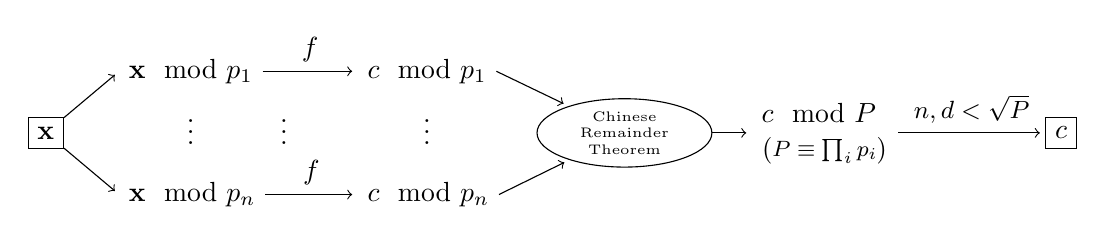
\begin{tikzpicture}[auto, node distance = 3cm,shorten >= 2pt]
      \node [rectangle, draw, text centered] (x) {$\mathbf{x}$};

      \node [above right = 0.3cm and 0.7cm of x] (xmod1) {$\mathbf{x}\mod p_1$};
      \node [right  of=xmod1] (cmod1) {$c\mod p_1$};

      \node [below right = 0.3cm and 0.7cm of x] (xmodn) {$\mathbf{x}\mod p_n$};
      \node [right  of=xmodn] (cmodn) {$c\mod p_n$};


      \node [below = 0cm of xmod1] () {$\vdots$};
      \node [below = 0cm of cmod1] () {$\vdots$};
      \node [below right = 0cm and 0.1cm of xmod1] () {$\vdots$};

      \node [ellipse, draw, text centered, right =6cm of x, node distance = 3cm, text width = 1.5cm, inner sep = 1pt] (crt) {\baselineskip=-10pt \tiny Chinese Remainder Theorem \par};
      \node [right = 0.5cm of crt] (cmodP) {\minibox{ $c\mod P$  \\ \footnotesize $\left(P\equiv\prod_i p_i\right)$} };

      \node [rectangle, draw, text centered, right of=cmodP, node distance = 3cm] (c) {$c$};


      \path [line,->] (x) -- (xmod1.west);
      \path [line,->] (x) -- (xmodn.west);

      \path [line,->] (xmod1.east) -- node [above]{$f$} (cmod1.west);
      \path [line,->] (xmodn.east) -- node [above]{$f$} (cmodn.west);

      \path [line,->] (cmod1.east) -- (crt);
      \path [line,->] (cmodn.east) -- (crt);

      \path [line,->] (crt) -- (cmodP);

      \path [line,->] (cmodP) -- node [above]{\small $n,d < \sqrt{P}$} (c);
    \end{tikzpicture}
  \end{center}
  \caption{The diagram representing rational reconstruction.}
  \label{fig:RatReconstr}
\end{figure}

\section{Solving Linear Systems of Equations}
For floating numerical stability is important.

For finite fields only field operations. PLU decomposition algorithm.

Put the one-loop cases here? Fourier transform and hard-coded solutions for inversions?

\section{On-Shell Loop Momenta and Finite Fields}
The extension of unitarity approaches to employ only operations
defined in an algebraic field was proposed 
in ref.~\cite{Peraro:2016wsq}.
A finite-field based calculation allows to compute exact values
for the integral coefficients $c_{\Gamma,i}$ of eq.~\eqref{eq:A}
in a numerical framework.
This idea
was applied recently in \cite{Badger:2017jhb,Abreu:2017hqn} for
pure gluon-scattering amplitudes, and here we discuss our
implementation for amplitude computations with fermions.

\subsubsection{Generic Algebraic Extension}

From here on we denote by $\mathbb{F}$ an arbitrary 
number field. In practice, we will be interested in
$\mathbb{F}$ being the field of rational numbers $\mathbb{Q}$
or the finite field $\mathbb{Z}_p$
of all integers modulo a prime number $p$.
In general, polynomial equations do not have solutions in 
$\mathbb{F}$. This is at odds with the fact that
in a unitarity-based approach one needs 
to generate loop momenta which satisfy a set of quadratic
conditions corresponding to setting propagators to zero.
%
In the presence of fermions, the situation becomes more 
complicated due to the extension of the Clifford algebra beyond 
four dimensions. More specifically, terms such as $\ell^\mu
\gamma_{[D_s]\mu}$ exhibit the $(D-4)$-dimensional
components of the loop momenta,
which are in general not 
$\mathbb{F}$-valued for on-shell momenta
(more concretely, if we work on the field of rational numbers
these components are in general irrational),
leading to terms in the sub-currents of the
Berends-Giele recursion that are not $\mathbb{F}$-valued. 
%
To address this issue,
we start with a parametrization of the on-shell spaces as in 
ref.~\cite{Abreu:2017hqn} but always use normalized basis
vectors. We write the two-loop momenta as
\begin{equation}
    \ell_1 = (\ell_{1,[4]}, \vec{\mu}_1)\,,\quad \quad \quad
    \ell_2 = (\ell_{2,[4]}, \vec{\mu}_2)\,, 
    \label{eq:loopmomenta}
\end{equation}
where we denote their $(D-4)$-dimensional components as 
$\vec{\mu}_1$ and $\vec{\mu}_2$. Next, we choose an orthonormal
basis $\vec{n}_i$ of the $(D-4)$-dimensional space with
$n_1$ in the direction of $\vec{\mu}_1$ and write
\begin{equation}
\vec{\mu}_1 = r_1 \vec{n}_1, \quad  \vec{\mu}_2 = \frac{\mu_{12}}{\mu_{11}} r_1 \vec{n}_1 + r_2 \vec{n}_2
  \quad \mathrm{where} \quad r_1 = \sqrt{\mu_{11}}, \quad r_2 = 
  \sqrt{\mu_{22} - \mu_{12}^2/\mu_{11}},
\end{equation}
with $\mu_{ij}=\vec{\mu}_i\cdot\vec{\mu}_j$.
In a theory containing only vector particles we only ever need 
the values $r_i^2$, which are $\mathbb{F}$-valued both on- and
off-shell \cite{Abreu:2017hqn}. In contrast, in a theory with
fermions, components of Berends-Giele currents will take the
generic form
\begin{equation}
  \label{eq:ExtendedAlgebra}
  a_{00} + a_{10} r_1 + a_{01} r_2 + a_{11} r_1 r_2, 
\end{equation}
which is not $\mathbb{F}$-valued.
In order to nevertheless be able to
work in the field $\mathbb{F}$,
we consider 
the algebra $\mathbb{V}$ over the field $\mathbb{F}$, with 
$\mathbb{V}$ the vector space spanned by the basis 
$\{r_0=1,r_1,r_2,r_1r_2\}$ and equipped with the standard
addition and multiplication.
All components of the Berends-Giele are elements 
in the algebra, and can thus be written as a linear combination
of the $r_i$ with $\mathbb{F}$-valued coefficients. More
concretely, this means we only need to determine the $a_{ij}$ 
in eq.~\eqref{eq:ExtendedAlgebra} which are $\mathbb{F}$-valued
by construction.

An important observation is that, although the coefficients 
$a_{10}$, $a_{01}$ and $a_{11}$ in 
eq.~\eqref{eq:ExtendedAlgebra} are non-zero in
intermediate stages of the calculations, they vanish
for the integrands of helicity amplitudes as defined in 
eq.~\eqref{eq:tensorDecomposition}. This cancellation of the
$r_i$ terms holds in the HV scheme and
is due to the projection onto the invariant tensors 
$v_n$ of eq.~\eqref{eq:tensorDecomposition}, 
which yields polynomials in the Lorentz invariants 
$\mu_{ij}$ at the integrand level
(see the discussion in section \ref{sec:ParamIntegrands}).


\subsubsection{Only Vector Particles}
%
In ref.~\cite{Abreu:2017hqn}, this was resolved
by making sure that all scalar products
between the momenta in the problem were $\mathbb{F}$-valued.


\subsubsection{Special Metric Signature}

Any Lorentz-invariant quantity such as helicity amplitudes (normalized by an appropriate spinor weight)
depends on the space-time metric tensor only through contractions with momenta and states of external particles.
Thus  without loss of generality we can choose to use an alternating metric signature $(+,-,+,-,\ldots)$
and modify external momenta such that all Lorentz invariants remain unchanged.

We then can parametrize the two-dimensional loop-momentum components
$\vec{\mu}_1$ and $\vec{\mu}_2$ as follows:
\begin{equation}
  \vec{\mu}_1(t)  = \frac{1}{2}\begin{pmatrix}
    t+\dfrac{\mu_{11}}{t} \\
    t-\dfrac{\mu_{11}}{t} \\
  \end{pmatrix}, \quad
  \vec{\mu}_2(t)  = \frac{\mu_{12}}{\mu_{11}}\vec{\mu}_1(t) - \frac{r}{\mu_{11}}~\frac{1}{2}\begin{pmatrix}
    t-\dfrac{\mu_{11}}{t} \\
    t+\dfrac{\mu_{11}}{t} \\
  \end{pmatrix},
  \label{eq:muparam}
\end{equation}
where $t$ is a free dimensionful parameter that leaves the scalar products
$r = \sqrt{\mu_{12}^2-\mu_{11} \mu_{22}}$ and 
$\mu_{ij} = \mu_i^1 \mu_j^1 - \mu_i^2 \mu_j^2$ invariant. %

This parametrization allows to reduce the size of the algebraic extension $\mathbb{V}$ generated by \cref{eq:ExtendedAlgebra},
which is a significant optimization of numerical evaluations.


\todo{Note on other possibilities to avoid solving on-shell conditions.}


\section{Exact Interpolation of Functions over Finite Fields}
\subsection{Univariate Polynomials}
\subsection{Multivariate Polynomials}




\chapter{Spinor-Helicity}
\label{chap:4dspinhel}

here describe four-dimensional spinor-helicity

\todo{denormalized spinors for finite fields}



\chapter{van Neerven-Vermaseren Basis}
In the van Neerven-Vermaseren (NV) construction
\cite{Neerven1984a}, the $D$-dimensional
space-time is decomposed into a physical space and its complement, the
transverse space. The NV construction is used for integrand
parameterizations \cite{Ellis:2007br,Ita:2011hi}. Consider $r$ inflow momenta $p_1,\dots,p_r$. The
physical space is then spanned by these $r$ momenta and has dimensions
$D_p=\min(D,r-1)$, since the $r$ momenta are in general linearly dependent and one degree of freedom is absorbed by momentum
conservation $\sum_{i=1}^rp_i = 0$. Whenever $r>D$, one can find
additional relations to reduce the higher point scalar integrals to
lower point ones \cite{Melrose1965}. For example, if $D=4$, one finds
a basis with a maximal rank of $4$. The physical space therefore forms
a lower dimensional subspace whenever $r\leq D$. The complent to the
physical space is called
transverse space and has dimension $D_t=\max(0,D-r+1)$, such that
\begin{align}
  D=D_p+D_t.
\end{align}
We assume that the momenta $p_1,\dots,p_r$ are ordered, such that the
first $D_p$ vectors are linearly independent. The corresponding dual
vectors are called $v_{1},\dots,v_{D_p}$. The transverse basis
vectors are denoted $n_{1},\dots,n_{D_t}$ and we have the following properties
\begin{align}
    n_i\cdot n_j &= \delta_{ij}, & n_i\cdot p_j &= 0,\\
   v_j \cdot n_i  &= 0, & v_j\cdot p_i &= \delta_{ij}.\notag
\end{align}
For the case that $r > D$, the space
is parameterized solely in terms of linearly independent vectors
$p_i$. 
 The metric tensor is thus decomposed in the NV basis as 
\begin{align}
  g^{\mu\nu} = \sum_{i=1}^{D_p}p_i^\mu v_i^\nu+\sum_{i=1}^{D_t}n_i^\mu n_i^\nu,
\end{align}
with the projector into the transverse space consquently given by
\begin{align}\label{eq:metricpron}
  (g_\perp)^{\mu\nu} \equiv  \sum_{i=1}^{D_t}n_i^\mu n_i^\nu = g^{\mu\nu}- \sum_{i=1}^{D_p}p_i^\mu v_i^\nu.
\end{align}
One can thus decompose the loop momentum in the NV basis as 
\begin{align}
  \ell^\mu = \sum_{i=1}^{D_p}(\ell\cdot p_i)
  v_i^\mu+\sum_{i=1}^{D_t}(\ell\cdot n_i) n_i^\mu,
\end{align}
with the projections of the loop momentum on the transverse space
$t_i(\ell) = (\ell \cdot n_i)$.  In actual computations with $D>4$, only a specific combination of the
projection on the transverse space is relevant. Since external
particles remain in $4$-dimensions, the additional components of the
loop momentum are only relevant in contractions of the loop momentum
with itself
\begin{align}
  \mu^2 = -\ell_{[D-4]}^2 \equiv \sum_{i=5}^D(\ell \cdot n_i)^2,
\end{align}
for explicit integer $D$-dimensions. Only this combination is of
relevance in $D\neq 4$-dimensional calculations. The $n_{i>4}$ are the transverse
vectors of the $D-4$-dimensional space. One can split up the
decomposition into a $4$-dimensional part and a $D-4$-dimensional part
and gets for the projector into the transverse space
\begin{align}\label{eq:metricprond}
\begin{split}
  (g_\perp)^{\mu\nu} &=  \sum_{i=1}^{D_t}n_i^\mu n_i^\nu=\sum_{i=1}^{4-r+1}n_i^\mu n_i^\nu +  \sum_{i=5}^{d}n_i^\mu n_i^\nu.
\end{split}
\end{align}



\chapter{Twistor Parametrization}
\todo{twistor parametrization} 
see e.g.\ Bobadilla thesis

%
%%% Literaturverzeichnis aus Datei "literatur"
%\phantomsection
%\nocite{apsrev41Control}
%\bibliography{zitationen,revtex-custom}
\bibliography{zitationen}

%
%%% Danksagungen aus Datei "src/danksag"
\chapter*{Acknowledgments\markboth{Acknowledgments}{}}
\addcontentsline{toc}{chapter}{Acknowledgments}
{
  \setlength{\parskip}{2pt}
  First of all, I would like to thank my first supervisor Harald Ita for his advice, guidance, fascinating insights
  and always giving me opportunities to grow as a researcher and giving me incentives to strive for higher standards.
  I am too very thankful to my second supervisor Fernando Febres Cordero for 
  being always ready to help me with all aspects of my doctoral studies,
  and letting me to ask all the question I ever wanted.
  I hope it was not too troublesome for you.

  I am very grateful to Ben Page and Samuel Abreu for patiently mentoring me,
  and very insightful discussions, research-related or otherwise.
  I cannot emphasize enough how valuable was it for me to have an opportunity to work by your side.

  I would like to thank my colleague Felix Anger, with whom I have been working closely in the first two years of my Ph.D studies.
  It has been a pleasure.

  My thanks go to Ekta Chaubey, Jerry Dormans, Michael Ruf, Wladimir Tschernow, Maximilian Klinkert, Harald Ita, Fernando Febres Cordero for critically reading parts of the manuscript and suggestions
  regarding the contents.

  I am also indebted to Ekta Chaubey for continuous encouragement, assistance, and for tolerating my complicated personality, especially during the time of writing this thesis. 

  I would like to thank Anna Gantimurova for supporting me in the first years of my doctoral studies.

  Finally, I would like to thank the ``Graduiertenkolleg 2044'' for providing a vibrant environment for carrying out Ph.D research,   
  and for the unique opportunity of having a framework of dialogue with our colleagues from experiments. 

  %GRK for framework, seminars and events


  %%%%%%%

  %First and foremost I would like to thank my supervisor Harald Ita, for his scientific guidance and his supportive attitude. Your advice and help has been invaluable! I would also like to express my gratitude to my second supervisor Fernando Febres Cordero, for the good collaboration and his outstanding commitment. I really enjoyed working with you! 

  %I would like to thank my collaborators Stefan H{\"o}che and Daniel Ma{\^i}tre, for the things I have learnt from them.

  %I would like to thank my colleague and office mate Vasily Sotnikov, for all the discussions and good collaboration on many aspects of this work. We have been a good team! To all the current and former members of the 8\textsuperscript{th} (and 7\textsuperscript{th}) floor for supporting me in one or another way but also for the good times shared: Kicker tournaments, Christmas parties and the ``Betriebsausflug'' come to my mind. A special thanks goes to Samuel Abreu for reading the manuscript of this thesis, to Matthijs van der Wild for forming the winning team of the kicker tournament '17 and to Jerry Dormans for tolerating our long discussions in the office but also for the fun in ``office 809''. To the members of the $\hbar$-racing team for the shared memories on snow and beyond: Lukas Altenkamp, Michele Boggia, Michael Kordovan.

  %I would like to thank Hannah Arnold, Giulia Gonella and Gernot Knippen for the shared time as student representatives of the ``Graduiertenkolleg 2044''. From organizing BBQs to increasing the ``educational value'' of the seminar series: I think we provided some innovative impulses!
}

%


%
%%% Ende des Dokuments
\end{document}
